\documentclass[tocnosub,noragright,centerchapter,fullpagesingle,12pt]{uiuc_csthesis18}

% Updated version of the ECE department's latex resources

% Use draftthesis for notes and date markings on every page.  Useful when you
%   have multiple copies floating around.
% Use offcenter for the extra .5 inch on the left side. Needed with fullpage and fancy.
% Use mixcasechap for compatibility with hyperref package, which does NOT like all caps default
% Use edeposit for the adviser/committee on the title page.
% Use tocnosub to suppress subsection and lower entries in the TOC.
% PhD candidates use "proquest" for the proquest abstract.

\makeatletter

\usepackage{setspace}
\usepackage{epsfig}  % for figures
\usepackage{latexsym}
\usepackage{graphicx}  % another package that works for figures
% \usepackage{subfigure}  % for subfigures
\usepackage{amsmath}  % for math spacing
\usepackage{amssymb}  % for math spacing
\usepackage{url}  % Hyphenation of URLs.
\usepackage{lscape}  % Useful for wide tables or figures.
\usepackage{booktabs} % For formal tables
\usepackage{multirow}
\usepackage{subcaption}
\usepackage[numbers]{natbib}
\bibliographystyle{unsrtnat}

\usepackage{capt-of}
\usepackage{cleveref}
\usepackage{comment}
%\usepackage{algorithm2e}
\usepackage{etoolbox,siunitx}
%\sisetup{round-mode=places,round-precision=3,table-format=1.2,detect-weight}
% \sisetup{separate-uncertainty,
%          table-figures-uncertainty=2,
%          table-number-alignment = center,
%         }
\usepackage{graphicx}
\usepackage[chapter]{algorithm}
\usepackage[normalem]{ulem}
\usepackage{array}
\usepackage{longtable}
\usepackage{setspace}

\usepackage{algpseudocode}
\renewcommand{\algorithmicrequire}{\textbf{Input:}}
\renewcommand{\algorithmicensure}{\textbf{Output:}}
\newcommand{\lnb}[1]{%
  \ln\mleft(#1\mright)%
}
\usepackage{mleftright}
\usepackage{bbm}
\usepackage{bm}
\usepackage{wrapfig}
\usepackage{float}
\usepackage{xfrac}
\usepackage[flushleft]{threeparttable}
\usepackage[super]{nth}

\newcommand{\ours}{FuseRec{}}
% Uncomment the appropriate one of the following four lines:
%\msthesis
\phdthesis
%\otherdoctorate[2]{DISSERTATION PROPOSAL}
%\othermasters[abbrev]{Title of Degree}

\title{Modeling effect of evolution and connections to user behavior}
\title{User latent behavior modeling in an interconnected world}
\title{User behavior modeling: Towards solving the duality of interpretability and precision}
\author{Kanika Narang}
\department{Computer Science}
\degreeyear{2020}

% Advisor name is required for
% - doctoral students for the ProQuest abstract
% - master's students who do not have a master's committee
\advisor{Hari Sundaram}

% Uncomment the \committee command for
% - all doctoral students
% - master's students who have a master's committee
\committee{Associate Professor Hari Sundaram, Chair\\
        Assistant Professor Alexander Schwing \\
        Professor ChengXiang Zhai \\
        Dr. Chris Brew} % etc.

\begin{document}

%%%%%%%%%%%%%%%%%%%%%%%%%%%%%%%%%%%%%%%%%%%%%%%%%%%%%%%%%%%%%%%%%%%%%%%%%%%%%%%
% COPYRIGHT
%
%\copyrightpage
%\blankpage

%%%%%%%%%%%%%%%%%%%%%%%%%%%%%%%%%%%%%%%%%%%%%%%%%%%%%%%%%%%%%%%%%%%%%%%%%%%%%%%
% TITLE
%
\maketitle

%\raggedright
\parindent 1em%

\frontmatter

%%%%%%%%%%%%%%%%%%%%%%%%%%%%%%%%%%%%%%%%%%%%%%%%%%%%%%%%%%%%%%%%%%%%%%%%%%%%%%%
% ABSTRACT
%
\begin{abstract}
% Put the abstract in a file called "abs.tex" and it'll be inputted here.
User behavior modeling has become an indispensable tool with the proliferation of socio-technical systems to provide a highly personalized experience to the users. These socio-technical systems are used in sectors as diverse as education, health, law to e-commerce, and social media.
The two main challenges for user behavioral modeling are building an in-depth understanding of online user behavior and using advanced computational techniques to capture behavioral uncertainties accurately.
This thesis addresses both these challenges by developing interpretable models that aid in understanding user behavior at scale and by developing sophisticated models that perform accurate modeling of user behavior.

Specifically, we first propose two distinct interpretable approaches to understand explicit and latent user behavioral characteristics.
Firstly, in \Cref{chap:evolution}, we propose an interpretable Gaussian Hidden Markov Model-based cluster model leveraging user activity data to identify users with similar patterns of behavioral evolution. We apply our approach to identify researchers with similar patterns of research interests evolution.  We further show the utility of our interpretable framework to identify differences in gender distribution and the value of awarded grants among the identified archetypes. We also demonstrate generality of our approach by applying on StackExchange to identify users with a similar change in usage patterns.

Next in \Cref{chap:reliability}, we estimate user latent behavioral characteristics by leveraging user-generated content (questions or answers) in Community Question Answering (CQA) platforms. In particular, we estimate the latent aspect-based reliability representations of users in the forum to infer the trustworthiness of their answers. We also simultaneously learn the semantic meaning of their answers through text representations. We empirically show that the estimated behavioral representations can accurately identify topical experts.

We further propose to improve current behavioral models by modeling explicit and implicit user-to-user influence on user behavior. To this end, in \Cref{chap:social}, we propose a novel attention-based approach to incorporate influence from both user's social connections and other similar users on their preferences in recommender systems. Additionally, we also incorporate implicit influence in the item space by considering frequently co-occurring and similar feature items. Our modular approach captures the different influences efficiently and later fuses them in an interpretable manner.
Extensive experiments show that incorporating user-to-user influence outperforms approaches relying on solely user data.

User behavior remains broadly consistent across the platform. Thus, incorporating user behavioral information can be beneficial to estimate the characteristics of user-generated content.
To verify it, in \Cref{chap:induced}, we focus on the task of best answer selection in CQA forums that traditionally only considers textual features. We induce multiple connections between user-generated content, i.e., answers, based on the similarity and contrast in the behavior of authoring users in the platform. These induced connections enable information sharing between connected answers and, consequently, aid in estimating the quality of the answer.
We also develop convolution operators to encode these semantically different graphs and later merge them using boosting.

We also proposed an alternative approach to incorporate user behavioral information by jointly estimating the latent behavioral representations of user with text representations in \Cref{chap:syntactic}. We evaluate our approach on the offensive language prediction task on Twitter. Specially, we learn an improved text representation by leveraging syntactic dependencies between the words in the tweet. We also estimate the abusive behavior of users, i.e., their likelihood of posting offensive content online from their tweets. We further show that combining the textual and user behavioral features can outperform the sophisticated textual baselines.

\end{abstract}


%%%%%%%%%%%%%%%%%%%%%%%%%%%%%%%%%%%%%%%%%%%%%%%%%%%%%%%%%%%%%%%%%%%%%%%%%%%%%%%
% DEDICATION
%
\begin{dedication}
% Whatever dedication you want.
%For those who tend to be forgotten.
To my parents for their love and support.
\end{dedication}

%%%%%%%%%%%%%%%%%%%%%%%%%%%%%%%%%%%%%%%%%%%%%%%%%%%%%%%%%%%%%%%%%%%%%%%%%%%%%%%
% ACKNOWLEDGMENTS
%
% Put acknowledgments in a file called "ack.tex" and it'll be inputted here.
\begin{acknowledgments}
This thesis has been made possible due to the contributions of many people.
First and foremost, I would like to express the sincerest gratitude to my advisor, Associate Professor Hari Sundaram, for his constant support and guidance.
My most prominent learning from his mentorship is his unique problem-solving skills and critical thinking.
His attention to detail, including presentation skills, has also improved clarity in my academic writing. With the independence afforded by him in my research, I was able to explore and work in diverse areas helping me become a more holistic researcher.

I also extend my heartfelt thanks to Assistant Professor Alexander Schwing for taking me under his wings and teaching me the ropes of deep learning. I appreciate him devoting so much time to mentor me even when our research interests did not align.
I thoroughly enjoyed working with him, and he is among the most optimistic and supportive people I know in academia.
Next, I would like to thank my committee members, Professor ChengXiang Zhai and Dr. Chris Brew, for their contributions to this thesis.
Prof. Zhai has taught me the importance of situating your research in the grand scheme of things. He has pushed me harder to think about the broader impact of my research that has dramatically improved the writing quality of this thesis. I also thank Dr. Brew for teaching me the importance of fundamental research and to being critical even of positive results.

I am also grateful to Assistant Professor Snigdha Chaturvedi and Dr. Susan Dumais for mentoring me in the initial years of my Ph.D. and providing an exemplar example of successful women researchers in the field. I feel fortunate to be advised by exceptional mentors in my career.
A big shout out to especially Professor Pankaj Jalote, Professor Ponnurangam Kumaraguru (PK), and Professor Mayank Vatsa at my undergraduate institution, Indraprastha Institute of Information Technology (IIIT-D), for igniting the flame of research curiosity in my formative years. My initial experiences during IIIT-D helped me appreciate the joys and importance of research and motivated me to pursue it as a full-time career.

Thanks also to my colleagues at Crowd Dynamics Lab for being my mentors, support system, and critiques of my research.
All my friends outside work also deserve a special mention for helping me maintain a semblance of a personal life beyond my research.

Finally, to my parents for believing in my dream and their continued love and support over the years. This acknowledgment will not be complete without mentioning my fianc\'e, Dr. Ketan Mittal. Thanks for being my pillar of strength and an ardent champion of my success throughout this time. I owe a great deal of this thesis to him.

\end{acknowledgments}

%%%%%%%%%%%%%%%%%%%%%%%%%%%%%%%%%%%%%%%%%%%%%%%%%%%%%%%%%%%%%%%%%%%%%%%%%%%%%%%
% TABLE OF CONTENTS
%
\tableofcontents

\mainmatter

%%%%%%%%%%%%%%%%%%%%%%%%%%%%%%%%%%%%%%%%%%%%%%%%%%%%%%%%%%%%%%%%%%%%%%%%%%%%%%%
% INSERT REAL CONTENT HERE
%

\chapter{Introduction}
\label{chapter:introduction}

Artificial Intelligence (AI) is a branch of computer science research that deals with the development of machines with intelligence rivaling those of humans. In other words, machines that can perform tasks that generally require human intelligence, such as visual perception, decision-making, speech recognition, and more.
Most of the current AI research is task-driven and has achieved or, in some cases, even surpassed human intelligence \cite{devlin2019bert, GoogleNet, PRelu, AlphaGo}. This advancement has resulted in the assimilation of AI into our life inadvertently, in the form of \emph{socio-technical} systems around us. These intelligent systems provide self-paced learning in the education sector \cite{education}, enable targeted marketing in e-commerce websites \cite{targeted}, facilitate personalized medicare unique to patient's body type, genetics, and lifestyle \cite{medicine} and even predict repeat crime incidence for bail seeking convicts \cite{bail}.

The success of these intelligent machines lies in the fact that they can understand and model complex human behavior effectively and use it to extend highly personalized solutions at scale.
Interactions or activities performed by the user on a specific platform characterize their behavior. For instance, in an e-commerce platform, activities denote items purchased by the user. Similarly, in a Community Question Answering (CQA) forum like StackExchange or Reddit, these activities are defined as posting questions or answers or voting on other user's answers.
Artificial Intelligence, or specifically user behavior modeling, sifts through vast amounts of past user data to find recurring patterns and predict user's future purchases, search intent, or information need \cite{search, SAS:2018, beutel}.

There are still many challenges abound to accurate modeling of user behavior.
These challenges primarily arise because humans are imperfect sensors of information. They do not necessarily conform to repetitive patterns and can be unpredictable. The user's behavior also tends to evolve. Besides, users are biased as they tend to get influenced by other users, their environment, or even exhibit unconscious biases. With that being said, the current scenario also affords many more opportunities that were not present before. First, due to the close intertwining of the technology with our lifestyle, we have abundant user interaction data available to us now, more than ever before. These vast reserves of longitudinal data can help the models to learn the nuances in the user behavior with more traces of behavioral change over time. Second, they are further aided by the concurrent improvements in computing power and computational techniques, such as deep neural networks, that can learn higher-degree polynomial functions needed to model and understand complex user behavior.

The philosophy of achieving at par human intelligence through AI is, in essence, to first understand how humans process and extract knowledge from their environment and then emulate that in machines. Thus, to build a comprehensive user behavior model, we need to both \emph{understand} their online behavior and use the learned insights to accurately \emph{model} the user activity data in the platform.

Recently proposed Deep Neural Networks (DNNs) are the class of AI algorithms that employ multiple layers to progressively extract more abstract and composite representations from the raw input, thus, removing the need for feature engineering. DNNs have also beaten human benchmarks in many language understanding and visual perception tasks \cite{gilbert2013widespread, GoogleNet}, but they are notorious for being uninterpretable.
The model interpretability is highly desirable as these models are used increasingly in sensitive and impactful domains like law and health.
Owing to the demand for explainable models, a recent class of works advocates using simple \emph{interpretable} models such as decision trees, linear regression for these domains \cite{learning}. On the other hand, model-agnostic approaches are also developed for interpreting these black-box neural models with techniques like feature importance or explaining individual predictions \cite{lime, interpretable}.
However, it is still challenging to achieve the dual objective of \emph{interpretability} and high \emph{precision} in a single model.
It thus creates a dichotomy between creating simpler models that offer a more in-depth understanding of the behavior versus using the advanced computational techniques
to capture behavioral uncertainties accurately.


\section{User Behavior Modeling}
The overall aim of this dissertation is to achieve both \emph{understanding} and an accurate \emph{modeling} of user behavior.
However, it is not easy to build \emph{interpretable} models that aid in understanding users and are also \emph{sophisticated} enough to capture behavior nuances precisely.
Thus, we propose to view the problem of user behavior modeling from multiple angles. Each perspective will lead us to a different class of solutions, all of them bringing us closer to the overall goal of improved user behavior modeling.

\subsection{Understanding user behavior}
An abundance of user activity data online presents tremendous opportunities to analyze user behavior unhindered in the real world. This activity data also often spans thousands or millions of users; a scale never achievable in field experiments. This opportunity has led to the emergence of an interdisciplinary field known as \emph{computational social science} that brought social scientists and computer scientists together. Researchers in this field use computational techniques to investigate behavioral relationships and social interactions in online platforms \cite{womenwiki, evaluating}. They typically assess the validity of previous social science theories to understand user online behavior at scale.

The first and foremost perspective, thus, draws from the field of computational social science. The works following this perspective should use advances in computational techniques to process vast amounts of user data and extract meaningful and comprehensible patterns of user behavior. These models, primarily aiming at providing an in-depth understanding of user behavior, thus fall into the category of \emph{interpretable} models. This interpretability often comes at the expense of model precision.

These models can also provide an excellent framework to perform additional hypothesis testing of correlation of user's behavior with other covariates that can be possibly predictive of their behavior. For instance, we can empirically test hypotheses like do changes in the posting pattern of a StackExchange user affect the upvotes their answers get? Furthermore, does that subsequently affect their activity level in the platform? These findings can be beneficial for moderators of the online communities to devise incentivization strategies to retain active users in the platform. Another interesting hypothesis worth investigating can be the correlation of change in the publication behavior of scholars with the amount of research grants awarded to them. These findings can be particularly attractive to grant-awarding institutions to ascertain any potential biases or merits in their current grant-awarding scheme.

Apart from discrete user activity data, there are massive amounts of multimodal user interaction data available in these platforms such as text, video, speech, etc.
User-generated textual data is the most popular form of interaction among them. Textual data is prevalent on multiple platforms such as reviews in e-commerce websites, questions, or answers text on CQA forums, tweets, or posts on social media platforms like Twitter or Facebook.

Textual data is more complex and sophisticated to comprehend than discrete activity features. Nevertheless, analyzing textual data opens the door to \emph{understanding} the extensive and latent characteristics of user behavior that are not even possible to comprehend with activity features. For instance, the text of user reviews can be used to learn user affinity to different aspects of the product, such as relative importance of different aspects-food, service, location of a restaurant for a particular user.
Similarly, the text of the user's answers or questions in a CQA forum can be used to discern latent features like the user's preferable topics to answer or their expertise for different topics. Prior works have leveraged the text of user's tweets or posts to understand user's political leanings \cite{political}, state of their mental health \cite{mentalhealth}, and much more. Thus, it is imperative to leverage user-generated content to create a comprehensive understanding of user behavior.

Finally, works following this line of research should build interpretable models using extensive user data to provide an in-depth understanding of user behavior at scale.

\subsection{Improving user behavioral models}
The technological advancement in precise modeling of user behavior has afforded us with the seamless integration of AI into our lives. These intelligent systems provide \emph{personalized} solutions at scale in sectors as diverse as e-commerce to education to medicine. Another complementary usage of creating powerful behavioral models is the ability to identify deviant users or even credible users on the platform. This outcome is highly desirable in the current circumstances, with the rise in illegitimate use of technology.

The second perspective, thus, mainly deals with
pushing the performance boundaries of the state-of-the-art user behavioral models.
Specifically, the solutions following this line of research strive to capture a comprehensive picture of user behavior by factoring in the myriad explicit and implicit influences on users. These methods can draw from a large body of social science research about user behavior in real-life settings. Note that the first perspective also deals with evaluating these theories in the online data traces with the primary aim of interpretability. As noted earlier, interpretability often occurs at the cost of model precision.
On the contrary, the primary aim of this line of research is to build sophisticated behavioral models that can predict future user behavior accurately. In fact, the second perspective follows from the first one as it can leverage an improved understanding of the user's online behavior to build precise behavioral models.

The works following this line of research need to tackle multiple challenges posed to accurate behavioral modeling. For instance, a user's behavior tends to evolve with experience. Similarly,  a user's friends, peers, or in general, other users with a similar background (demography, preferences, etc.) often influence their behavior. It is now possible to computationally model these effects due to the availability of extensive user interaction data on the online platforms. For instance, long-term user data provides the opportunity to model patterns of change in user behavior with time. Similarly, user-to-user influences manifest in many of the current online platforms due to their prevalent social structures. Connected users, i.e., users with established trust or friend relationships on these platforms, are empirically shown to exhibit similar behavior online, a phenomenon popularly known as user homophily \cite{Tang:2009}.

Further, users hold an unconscious bias towards users with a similar background; a phenomenon also reverberated online. For instance, a user may trust movie recommendations of another user with similar demographics (same age or gender). Similarly, an Indian user may trust the ratings of another Indian user more than a non-Indian user when evaluating an Indian restaurant. Thus, it is crucial to capture these implicit influences
between users who are alike based on general notions of similarity, such as demography or activity in the platform.
Capturing the implicit influence is more complicated than explicit influence, but it can provide vital cues for predicting the behavior of users with \emph{few} social connections.
They can also be particularly helpful in online platforms with no established social structure such as review platforms or CQA forums.

Thus, the creation of models that capture the explicit and implicit influences on users efficiently and at scale is prudent to bring advancement in the field of user behavior modeling.

\subsection{Incorporating user behavior as metadata to improve complementary tasks}
Most of the current research related to user behavior modeling intends to model or predict user behavior primarily.
However, there are related tasks pertinent to the estimation of characteristics of the user-generated content in the online platforms.
Some of the examples of such related tasks are estimating the quality, credibility, or profanity of the content online.

Current work solving these tasks merely exploits the data features and completely ignores the user information. Users are the creators of the content, and their behavior remains broadly consistent across the platform. Thus, adding contextual information about user behavior estimated from their actions in the platform can immensely improve the prediction task.
For instance, current models proposed for prediction tasks like credible answer selection on CQA forums or hate speech prediction utilize the semantic meaning of the text to make such predictions \cite{zhang2018texttruth, elsherief2018hate}. However, user expertise estimated through their prior answers on the platform can be used to differentiate between users. This differentiation can consequently help to rank user-provided answers based on their trustworthiness.
Similarly, the abusive behavior of users estimated from their prior content can provide a useful precedent when predicting the offensive nature of their new content. Furthermore, utilizing user homophily, behavioral priors of users can be shared amongst explicitly and implicitly similar users.

Thus, in this perspective, we propose to build models that leverage information about commonalities and disparities in user behavior to improve prediction tasks about user-generated content.

\noindent
\section{Thesis Contributions}
We outlined three different perspectives to solve the problem of user behavior modeling.
These different perspectives are in no means comprehensive. However, they pave a viable way to ultimately develop models than can attain the twin goal of interpretability and precision.
Since the field of user behavioral modeling is massive, there are numerous unsolved challenges within each perspective. In this dissertation, we propose a few foundational works under each perspective that provide potential approaches to solve these posed challenges.
Specifically, we attempt to answer the dichotomy of understanding versus modeling user behavior by proposing interpretable models that primarily aim to provide detailed insights about user online behavior. Further, we develop frameworks to model user behavior accurately or leverage information about user behavior to improve prediction tasks related to user-generated content.

\subsection{Understanding user behavior}
Under this perspective, we propose two works, the first one that directly models user activity data to understand patterns of behavioral change and another that leverages user-generated content to understand the latent characteristics of user behavior.

Firstly, in Chapter \ref{chap:evolution}, we leverage user activity data to understand the behavioral evolution of individuals with experience.
We introduce an interpretable Gaussian Hidden Markov Model (G-HMM) cluster model to identify archetypes of evolutionary patterns among users.
Specifically, we apply our model to discover archetypical patterns of research interests' evolution among Academics and patterns of change in activity distribution of users of Stack Exchange communities. Our model allows us to correlate user behavior with external variables such as gender, income, etc.

In \Cref{chap:reliability}, we leverage the content of the user's answers in CQA forums to learn latent characteristics of user behavior--\emph{latent reliability}. We use this latent behavior representation to solve the task of ranking answers of a given question based on its trustworthiness. This ranking is especially vital as CQA forums are crippled with rampant unreliable content on their platform due to almost no regulations on post requirements or user background. Thus, this misinformation severely limits the forum's usefulness to its users.

We propose an unsupervised framework to learn the latent characteristic of user behavior--reliability and latent characteristic of answers--trustworthiness in a mutually reinforcing manner.
In particular, our model learns a user representation vector capturing her reliability over fine-grained topics discussed in the forum. Besides, we also learn the semantic meaning of comments and posts through text-aware text representations or word embeddings.
The learned latent representations using text affords an in-depth understanding of user reliability, improbable to comprehend using discrete activity data.



\subsection{Improving user behavioral models}
There are multiple unsolved challenges for accurate modeling of user behavior online.
In this dissertation, we focus on capturing the user-to-user influence to improve user behavioral models.
These influences can be either explicit in terms of social connections present in the platform itself or implicit in the absence or sparsity of established social connections.
We propose to capture the implicit social influence, measured either through similarity or contrast in users' behaviors, by inducing connections between them. These connections enable information sharing among connected users resulting in an improved model of their behavior.

We use \emph{Graph Convolution Networks} (GCN) \cite{gcn} to model both explicit social connections and induced connections between users.
GCN is a recent class of neural networks that learns node representations in graph-structured data. Specifically, the model aggregates representations of the node itself, along with its neighbors, to compute a node representation. The model is very efficient with parallel batch processing and sparse computations. Thus, it can scale to large scale user graphs present on online platforms.

Recommender Systems have previously exploited the user homophily (similar behavior) between connected users to provide improved recommendations to their users \cite{Diffnet, SBPR, GRU4Rec}.
Thus, in Chapter \ref{chap:social}, we propose to incorporate the effect of \emph{user-to-user influence} on the user's behavior in a recommender system.
In this work,
we exploit homophily in both user and item space.
In the user space, apart from a user's explicit social connections in the platform, we also induce connections between users with a similar purchasing history.
In the item space, we construct a 'social graph of items' based on similarity in item features and co-occurrence in the dataset.
These implicit similarity connections between items help the model to handle data sparsity in items (long-tail items, i.e., items with limited training data).

We propose a novel graph attention-based aggregation models to estimate social influence in both user social and item similarity graphs. Besides, we also learn explicit attention weights for each pair of connected nodes to capture varying influence strengths on the behavior. We finally propose an interpretable aggregation approach to combine the different factors influencing user preferences.

\subsection{Incorporating user behavior as metadata to improve complementary tasks}
Under this perspective, we leverage user behavior information to aid in two diverse prediction tasks related to user-generated content. In addition, we propose distinct techniques to include user behavioral information for each task. The first approach incorporates the user behavioral information by inducing connections amongst user-generated content. Induced connections aid in information sharing resulting in improved predictions. The second technique, on the other hand, learns powerful user representations encapsulating users' behavior. We subsequently use these representations in addition to the textual features to improve the prediction task.

CQA forums suffer from abundant low quality content and answer selection task, thus, aims at identifying the best answer out of the given answers to a question. Current approaches predict answer quality in isolation of the other answers to the question and user activity across the forum (other posted questions or answers).
Thus, in \Cref{chap:induced},
we induce connections based on both similarity and contrast between users' behavior (answers) to share user behavioral information among answers.

Specifically, we induce a contrastive graph between user-provided answers replying to the same question and a similarity graph between answers across different questions if the replying users are exhibiting similar behavior. We also propose a modification to the original GCN to encode the notion of contrast between a node and its neighborhood.
Besides, we use state-of-the-art text representation learning approaches to compute representation for the user's answers and questions. We subsequently induce connections between user-generated answers based on these text representations.
Finally, multiple graphs expressing semantically diverse relationships are merged through an efficient boosting architecture to predict the best answer.

Thereafter, in \Cref{chap:syntactic}, we work on
leveraging textual features along with user features
to detect the offensive language in tweets. Abusive behavior is rampant online and is affecting the experience of a large number of users on the platform. Hate attacks are often expressed in a sophisticated manner in the text (long clauses or complex scoping); thus, traditional sequential neural models are unable to capture them effectively.
In this work, we learn an improved text representation of the tweets
by leveraging syntactic dependencies between words.
We achieve this by inducing a graph on the words of a tweet where edges represent a dependency relationship. We use these representations subsequently to estimate a user's latent abusive behavior, i.e., their likelihood of using offensive language online.
Further, to capture homophily in abusive user accounts, we propagate this latent behavior through the user's social graph on Twitter. This user behavior information, in addition to the improved text representation of the tweet, dramatically improves the performance of offensive language detection models.
	% for INTRODUCTION in "intro.tex"
\chapter{Literature Review}
\label{sec:related}

Before delving into details of our proposed approach, we first discuss prior literature related to User Behavior Modeling in Online Social Networks, Academic Dataset and Recommender Systems. We also review text representation approaches used in Community Question Answering (CQA) forums and for short text in Twitter. We also briefly review recently proposed Graph convolution networks to model graph-structured data (used in our work) for these platforms.

\section{Online Social Networks}
There has been a lot of interest in the past on identifying and characterizing user behavior in online social networks (OSNs). \citet{Maia:2008} identified five distinct user behaviors of YouTube users based on their individual and social attributes. While \citet{Mamykina:2011} identified user roles based on just answer frequency in StackExchange. \citet{Adamic:2008} and \citet{Furtado:2013} worked on similar user behavioral studies on Yahoo Answers and Stack Overflow datasets, respectively. All these studies, however, ignore \emph{temporal changes} in the behavior and use engineered features for behavior modeling.

Some behavioral studies do model evolution of user activities in the platform too. \citet{Benevenuto:2009} learned a Markov model to examine transition behavior of users between different activities in Orkut in a static snapshot. \citet{Yang:2014} and \citet{Knab2003} proposed generative models that assigned each user action to a progression stage and classify event sequences simultaneously. They used their model to predict cancer symptoms, or products user would review in the future. However, the model did little to provide meaningful and interpretable stages and clusters. \citet{Angeletou:2011} constructed handcrafted rules to identify user roles and studied the change of user roles' composition in the community over time. Recently, \citet{Santos:2019} identified four distinct types of user activity pattern based on their activity frequency.

The Hidden Markov Model (HMM) has been widely used to model and cluster time sequences \citep{Smyth:1997, Bicego:2003, Coviello:2014} in the past. However, most of these models learn an HMM for each user sequence and then employ clustering algorithms to cluster the learned HMMs. These approaches are not scalable, and the clusters thus identified are not interpretable.

\section{Recommender Systems}
In the following section, we provide a brief review of approaches that model users' historical interactions to improve recommender systems. We first enlist approaches assuming static user behavior (Collaborative Filtering). Consequently, we review approaches that model the evolution of user behavior (Temporal Recommendation), social influence (Social Recommendation), and few recently proposed methods which are looking at combining the two (Socio-Temporal Recommendation).

\noindent
\emph{Collaborative Filtering:}
Collaborative Filtering (CF) is one of the most popular techniques for user modeling in recommender systems.
Specifically, the methods employ Matrix Factorization (MF) to decompose a user-item rating matrix into user and item specific latent factors.
Classical and seminal work for MF-based recommender systems~\cite{Rendle} uses a Bayesian pairwise loss (BPR). Collaborative filtering is also performed in item space~\cite{itemCF}, where similar items are computed offline based on their rating similarity or co-occurrence in the dataset. Consequently, it recommends items similar to the ones used in the past by the user.
Neural net approaches have been proposed recently to improve MF models. They learn more complex non-linearities in the user-item interaction data~\cite{NeuMF, CDAE}.

However, most MF approaches assume a static user-item interaction matrix. Often, this assumption is not accurate, particularly for online communities where user preferences evolve over time --- sometimes quickly --- necessitating temporal recommendation.

\noindent
\emph{Temporal Recommendation:}
There has been significant work in the area of temporal recommender systems that model a user's past interactions to inform a user's current preference. These temporal models generally assume a linear relationship between the events and model it using a Markov chain~\cite{FPMC, Rendle2}. However, these are often `shallow' (i.e., linear) methods that are inept at modeling the more complex dynamics of temporal changes. Recent works~\cite{Sun:2018, Cai:2017, SAS:2018} use deep net approaches involving convolution layers, attention networks, and recurrent neural nets to model complex relations. For example,~\citet{Caser} applies convolutional filters on the embedding matrix computed from a few recent items of a user. This model captures a higher-order Markov chain, but it still has a limited scope as it does not consider the entire history of a user.
In contrast, to model long term dependencies,~\citet{GRU4Rec} propose to model a user's sequential behavior within a session using recurrent neural nets. \citet{RRN} apply a recurrent architecture to both user and item sequences and hence model dynamic influences in popularity of movies on users' viewing preference. \citet{SAS:2018} instead employ a self attention module for next item recommendation that adaptively learns the importance of all past items in a user's history. However, these models are limited as they do not leverage the social connections of a user.

\noindent
\emph{Social Recommendation:}
Social recommenders integrate information from a user's social connections to mitigate data sparsity for cold-start users, i.e., users with no or minimal history. They exploit the principle of social influence theory~\cite{Tang:2009}, which states that socially connected users exert influence on each other's behavior, leading to a homophily effect: similar preferences towards items. \citet{SocialMF, SoReg} use social regularization in matrix factorization models to constrain socially connected users to have similar preferences. The recently proposed SERec~\cite{SERec} embeds items seen by the user's social neighbors as a prior in an matrix factorization model. The SBPR model~\cite{SBPR} extends the pair-wise BPR model to incorporate social signals so that users assign higher ratings to items preferred by their friends. However, these models assume equal influence among all social neighbors. TBPR~\cite{TBPR} distinguishes between strong and weak ties only when computing social influence strength.

\noindent
\emph{Socio-Temporal Recommendation:}
Few of the recent approaches have started to look at merging temporal dependence with social influence. \citet{Cai:2017} extend Markov chain based temporal recommenders~\cite{Rendle2} by incorporating information about the last interacted item of a user's friends. This work assumes markov dependence i.e. the future item just depends on the current item. This assumption is limiting im modeling evolving user preferences.

In the context of session-based recommendation, \citet{Sun:2018} propose a socially aware recurrent neural network that uses a dynamic attention network to capture social influence. On the other hand, \citet{Song:2019} use graph attention nets to model social influence on a user's behavior in the session. Both these models learn a unified user representation based on social influence with a user's temporal history.


\section{Scholarly Data}
Most of the work on user behavioral mining concerns career movement within academia. \citet{deville:2014} observed that transitions between academic institutions are influenced by career stage and geographical proximity. While \citet{clauset:2015} found that academic prestige correlates with higher productivity and better faculty placement. Recently, \citet{Danai:2018} studied career transitions across academia, government, and industry for Computer Science researchers. \citet{dashun:2013} proposed a statistical model to predict the most impactful paper, in terms of citations, of scientists across disciplines. They argued nonexistence of a universal pattern and showed that highest-impact work in a scientist's career is randomly distributed within her body of work.

Recent studies also looked at gender differences in funding patterns, productivity, and collaboration trends in academia \citep{Way:2016, Way:2017}. \citet{Way:2016} did not observe any significant difference across gender in hiring outcomes in academia. However, they showed that indirect gender differences exist in terms of productivity, postdoctoral training rates, and in career growth. Some earlier studies also reported gender differences in academia. \citet{Kahn:1993} identified gendered barriers in obtaining tenure for academics in economics, while \citet{Ward:2001} found gendered differences in pay related to publication record.

There also has been considerable interest in mining scholarly data produced by researchers (bibliographic data, researchers' usage of social media, etc.). Prior studies have looked at the evolution of research interests on a community level. \citet{liu2014chi} studied the evolution of research themes in articles published in CHI conference on Human Computer Interaction through co-word analysis. They highlighted specific topics as popular, core, or backbone research topics within the community. While \citet{Biryukov:2010} compared different scientific communities in DBLP dataset in terms of its interdisciplinary nature, publication rates, and collaboration trends. They also studied the variation of author's productivity with career length and observed that most of the authors have a short career spanning less than five years. \citet{Chakraborty:2018} studied trajectories of successful papers in computer science and physics by analyzing paper citation counts. They classified these trajectories into multiple categories including early riser, a late riser, steady riser, and steady dropper.

\section{Community Question Answering Forums}
Community Question Answering forums are increasingly used to seek advice online; however, they often contain conflicting and unreliable information. This misinformation could lead to serious consequences to the users. Thus, most of the work that model user behavior in CQA forums deals with predicting user reliability or quality of posted answers to a question.

Prior works can be classified into Feature-driven models; which use user and content-based engineered features for the task; another is Deep Text models that only model relevance of the content of question and answers for prediction and disregard user information. Recently, unsupervised approaches based on Truth Discovery principle are applied to model user expertise and answer quality simultaneously in these forums.

\noindent
\emph{Feature-Driven Model:}
Feature-driven models \cite{BurelMA16} develop features from three different perspectives: user features, content features, and thread features.
These features are fed into classifiers, such as tree-based models \cite{BurelMA16, JendersKN16, TianZL13} to identify the best answer. \citet{TianZL13} found that the best answer is usually the earlier and most different one, and tends to have more details and comments. \citet{JendersKN16} trained several classifiers for online MOOC forums. Different from existing works, \citet{BurelMA16} emphasize on the thread-like structure of question \& answer and introduce four thread-based normalization methods. These models predict the answer label independently of the other answers for the question.
CQARank leverages voting information as well as user history and estimates user interests and expertise on different topics ~\cite{yang2013cqarank}. \citet{barron2015thread} also look at the relationship between the answers, measuring textual and structural similarities between them to classify useful and relevant answers. All these supervised approaches need a large amount of labeled training data ~\cite{wen2018hybrid, mihaylova2018fact,oh2013finding}. However, it is expensive and unsustainable to curate each answer manually for training these models. Alternatively, forums employ crowd sourced voting mechanisms to estimate information reliability but it could lead to under-provision \cite{gilbert2013widespread}.

\noindent
\emph{Deep Text Models:} Text-based deep learning models learn an optimal representation of question-answer text pairs suitable to select the best answer \cite{ZhangLSW17, WuWS18, WangN15}. In SemEval 2017 on Community Question Answering (CQA),~\cite{nakov2017semeval} developed a task to recommend useful related answers to a new question in the forum.
SemEval 2019 further extends this line of work by proposing fact checking in community question answering~\cite{Mihaylova2019semeval}. \citet{FengXGWZ15} augment CNN with discontinuous convolution for a better vector representation; \citet{WangN15} uses a stacked biLSTM to match question and answer semantics. \citet{SukhbaatarSWF15} use attention mechanism in an end-to-end memory framework. Text-based models take longer to train and are computationally expensive.

\noindent
\emph{Truth discovery:} Different approaches based on truth discovery principle have been proposed to address predict answer quality in CQA forums~\cite{zhang2018texttruth, li2015discovery, zheng2017truth,li2016crowdsourcing,mukherjee2016truthcore,vydiswaran2011content}. Many truth discovery approaches are tailored to categorical data and thus assume there is a single objective truth that can be derived from the claims of different sources \cite{li2016survey}. Faitcrowd~\cite{ma2015faitcrowd} assumes an objective truth in the answer set and uses a probabilistic generative model to perform fine-grained truth discovery. It jointly models the generation of questions and answers to estimate the source reliability and correct answer. On the other hand,~\citet{wan2016truth} propose trustworthy \emph{opinion} discovery where the true value of an entity is modeled as a random variable with a probability density function instead of a single value.

Some truth discovery approaches also leverage text data to identify correct responses better.~\citet{li2017reliable} proposed a model for capturing semantic meanings of crowd provided diagnosis in a Chinese medical forum. In particular, they use a medical-related dictionary to extract terms in the response text and learn their semantic representations to discover trustworthy answers from non-expert users in crowdsourced diagnosis.
\citet{zhang2018texttruth} proposed a Bayesian approach to capture the multifactorial property of text answers and used semantic representations of keywords to mitigate the diversity of words in answers. To model the user reliability, the authors proposed a two-fold reliability metric that uses both false positive and true positive rates. These approaches only use certain keywords for each answer and are thus, limited in their scope.


\section{Twitter}
Most previous methods for detecting offensive speech on Twitter rely entirely on the textual content.
Most of these prior work includes using statistical features like bag-of-words or tf-idf features for automated detection.\citet{wulczyn2017} used character n-gram features for detecting abusive comments in the discussion on Wikipedia pages. On Twitter dataset, \citet{waseem-hovy-2016} used character and word n-gram features along with lexical and users features to detect hate speech. \citet{davidson2017automated} worked with character n-grams on a different Twitter dataset to achieve competitive performance. On the other hand, \citet{nobata} combined n-grams features with linguistic, syntactic, and semantic features. However, they observed that n-gram features are most beneficial for the detection task.
Even though bag-of-words approaches perform well, they are unable to capture nuanced hate speech as they fail to contextualize the word meanings.
For instance, depending on the context, the word \emph{gay} can be used to denote either ebullience or sexual preference. Only the latter is a candidate attack.

Recently, deep learning models are also proposed that leverage pre-trained word embeddings such as word2vec \cite{mikolov2013distributed} and Glove \cite{glove}
to capture aspects of the semantics of the tweets. These models aggregate individual word embeddings in a context-aware manner to compute tweet embeddings and later use them for classification.
\citet{gamback} and \citet{park2017one} used the Convolutional Neural network to compute the tweet embeddings while \citet{badjatiya2017deep} and \citet{agrawal} showed that Gated Recurrent Units or Long-Short Term Memory networks are useful to compute these embeddings.
On the other hand, \citet{ziqicnn} used a combination of CNNs and GRU to achieve competitive performance.

The syntactic structure of the text can also be used to help identify the target group and the intensity of hate speech. For instance,~\citet{warner2012} extracts POS-based trigrams such as DT jewish NN to extract hate speech against a specific target, Jews. While, \citet{silva2016} extends it further to look for generic syntactic structures like "I $<$intensity$>$ hate $<$target$>$'.
The primary difficulty of this work is that the space of possibly relevant rules is too large for an analyst to be confident that the list is truly comprehensive.
In addition, it verges on the impossible to specify a set of rules that will do a decent job on the endless variety of possible implicit attacks.

A minority of approaches take advantage of non-textual user data in addition to the text.
\citet{2017improved} added randomly-initialized user embeddings to their RNN model to obtain higher accuracy.
\citet{qian2018} showed that incorporating intra-user and reinforced inter-user representations significantly improve the performance of their bi-directional LSTM model. However, both of these approaches work on the individual user level and ignore the social influence on their behavior. \citet{mishra2018} captured the social influence in abusive accounts by computing a representation of a user's neighborhood through node2vec features.  The classifier described in \citet{mishra2019abusive} extends the previous paper by computing a user representation from an extended graph of users and tweets.


\noindent
\section{Graph Convolution Networks}
More recently, Graph Convolution Networks (GCNs) have been proposed to learn embeddings for graph-structured data~\cite{Kipf:2016}. Graph Convolution can be applied in both spatial and spectral domains to compute node representations. The learned node representations are then used for various downstream tasks like node classification \cite{gcn}, link prediction \cite{relationalGCN}, multi-relational tasks \cite{rase} etc. Spatial approaches employ random walks or k-hop neighborhoods to compute node representations  \cite{DeepWalk, node2vec, Planetoid, LINE}. Pioneer works on graph convolution in the spectral domain use fast localized convolutions ~\cite{deferrard, duvenaund}. Recently proposed Graph Convolution Networks~\cite{gcn} outperforms spatial convolutions and are scalable to large graphs. Various extensions to the GCN model have been proposed for signed networks \cite{signedgcn}, inductive settings \cite{graphsage} and multiple relations \cite{DualGCN, relationalGCN} and evolution~\cite{dysat}. All of the GCN variants assume label sharing as they assume similarity between connected nodes.

In Recommender Systems, GCNs have been used to model the user-item interaction graph. GCMC~\cite{GCMC} extends GCN by training an auto-encoder framework on a  bipartite user-item interaction graph that performs differentiable message passing, aggregating data from a user's and an item's 'neighbors'. PinSage~\cite{PinSage} proposed a random walk based sampling of neighbors to scale GCNs to web scale graphs. \citet{fan2019} further extend these methods to incorporate information from a user's social connections.
Similarly, \citet{Diffnet} use graph neural networks to model diffusion of social influence in recommender systems.

However, these methods either do not take a user's social neighbors into account or operate on static features.  All these models also assign uniform weight to all their neighbors, which does not represent online social communities well. Typically in these communities, some friends are only superficially known while others are known personally for years. Thus, they exert a different degree of influence on a user's behavior. Graph Attention Networks~\cite{GAT} can capture the varying influence stengths as they learn attention weights between each pair of nodes in a static graph.


\chapter{Discovering archetypes of behavioral evolution}
\label{chap:evolution}
In this chapter, we aim to discover archetypical patterns of behavioral evolution among users. In our work, an archetype comprises of \emph{progressive stages} of distinct research \emph{behavior}. We introduce a novel Gaussian Hidden Markov Model (G-HMM) cluster model to identify archetypes of evolutionary patterns. G-HMMs allow for: behavioral variation and different evolutionary rates; impose constraints on how individuals can evolve; and are interpretable.

We evaluate our approach to an interesting domain of patterns of change in research interests of scientists with experience. In addition, we evaluate our model for activity distribution evolution of users in StackExchange communities to showcase the generality of our framework \cite{evolution}.


\section{Overview}
\label{sec:Introduction}
In this chapter, we develop models to understand how individuals evolve with experience in social networks. The problem is important: as individuals interact with each other, they gain in experience, and behavioral changes reflect the newfound experience. However, despite a significant focus on community discovery and their evolution in social networks, our understanding of individual evolution is limited (\citet{Yang:2011, McAuley:2013} are some notable exceptions). Understanding evolutionary patterns, in general, is useful in a variety of applications: language evolution~\citep{Danescu}; expertise evolution~\citep{McAuley:2013}; journey optimization in digital advertising platforms.


Our specific interest lies in understanding how academics change their research behavior with gain in research experience. In the academic community, authors' research interests are influenced by other authors' directly (collaboration) or indirectly (related published research) and in general, by the current research trends in the community. Analyzing the evolution of academic behavior on the community level has attracted persistent interest; previous works studied the evolution of research themes for a particular scientific community \cite{Li:2011} or multiple communities \cite{Biryukov:2010, tanmoy:2013}.
On an individual level, evolutionary studies have looked at modeling career transitions \cite{Danai:2018}, citation evolution \cite{dashun:2013} and  productivity or collaboration trends \cite{Way:2017}. On the other hand, in this work, we want to identify dominant patterns of \emph{research interests} evolution common among academics across different subfields. Our work can help to answer questions like, Do academics focus on a single research area throughout their career or they venture in multiple areas as they gain experience? If they work on multiple areas, when does this shift usually happens? Are some evolutionary patterns preferred over the others? This knowledge can assist in providing better career guidance to junior faculty on how to structure their career. Moreover, it can help funding agencies identify researchers of particular evolutionary pattern that may need more assistance.


At the outset, discovering patterns of individual evolution appears to be a combinatorial problem: academics vary in not only the sub-field that they choose to start but also in subsequent areas of interest. Furthermore, their research interests may evolve at different rates. Despite variations in the chosen sub-field of an academic, and how academics can evolve, we observe regularities at different stages of their career. For instance, for an academic, transition through different stages--- Ph.D. Student (focusing on a single research area), being an assistant professor (working on few highly related areas) to eventually post-tenure (multiple areas, interests in multidisciplinary collaborations, etc.)---mark changes in research behavior. These elementary behavioral evolutionary patterns are visible in almost all academic fields, suggesting that surface variations (i.e., area of research for an academic) hide deeper regularities in patterns of behavioral change. We refer to these \textit{latent} regularities in individual behavior as \textit{behavioral stages}. We refer to the dominant progression patterns through behavioral stages as \textit{archetypes}. Note that researchers may evolve at different rates through these stages. We show that we can explain all individuals' surface variations (the observed research area on which the academic focuses) with a small set of such archetypes. ~\Cref{fig:example} shows a stylized example.

Thus a model for learning archetypes needs to: express variation in observable research behavior while exhibiting latent stochastic regularities governing the change of behavior. Furthermore, the model should allow individuals to evolve at different rates. Finally, the results ought to be interpretable in a post-hoc manner.

\begin{figure}
 \centering
  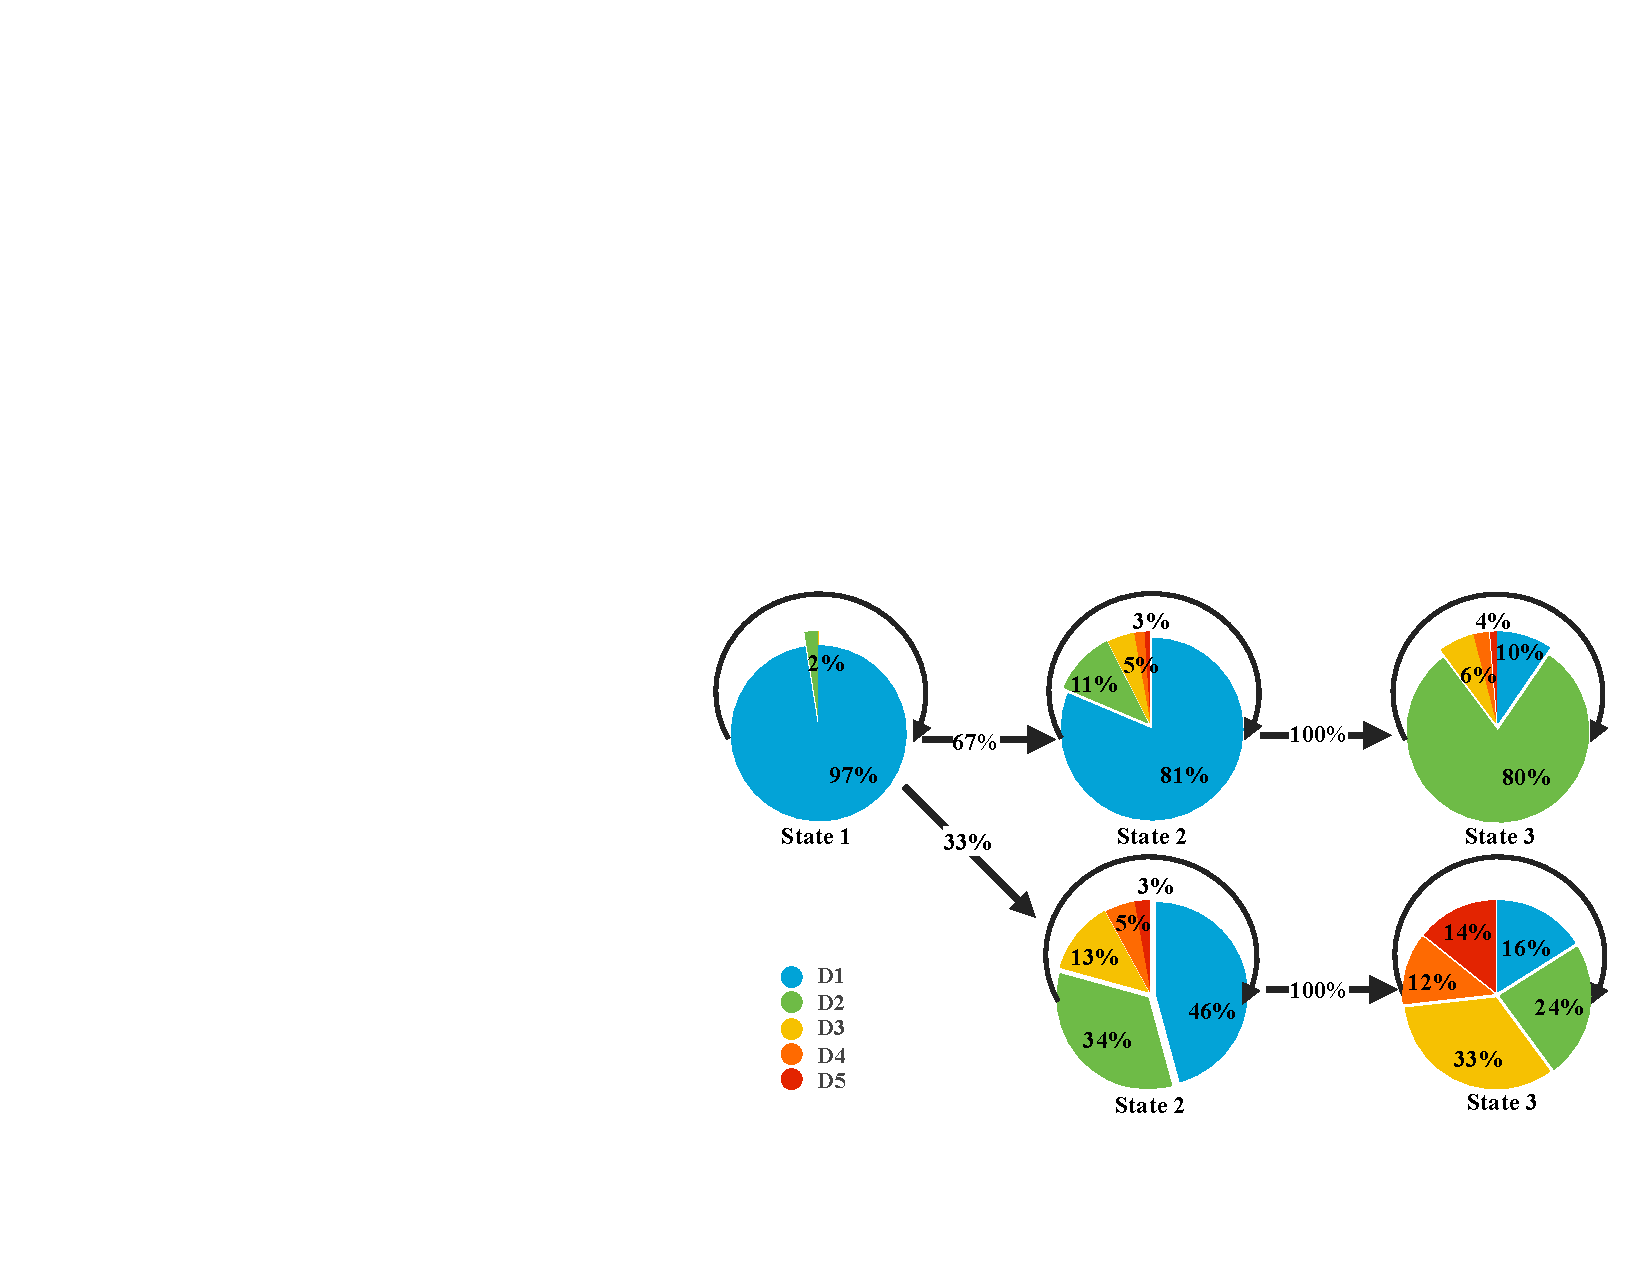
\includegraphics[width=0.7\linewidth,height=6.4cm]{figures/Example_figures_Self.pdf}
 \caption{\label{fig:example} A stylized academic evolutionary trajectory. Each pie chart is a \emph{behavior stage} in the trajectory. The numbers in each pie-chart show the fraction of chapters published in each research area \textit{$D_m$} in that stage. We use a normalized representation focused on the change of areas: the label $D_1$ represents the first research area of every academic, $D_2$ the second research area, etc. Normalized representations allow us to discover commonalities in behavioral changes of academics across seemingly unconnected domains. In this example, the top group of researchers evolves to shift their research focus to a new domain while the bottom group becomes increasingly interdisciplinary.
 }
\end{figure}

\noindent
Our work makes the following contributions:
\begin{description}
\item[A framework for modeling evolutionary trajectories:] We propose a sophisticated framework to identify dominant, interpretable, evolutionary archetypes amongst academics for modeling the evolution of their research interests. In contrast, prior work on academics has either focused on the qualitative analysis (e.g.,~\citep{Ward:2001}) or predicting career transitions~\citep{Danai:2018}. In our work, we assume that an archetype is a \emph{probabilistic model} that encodes individual progression through stages of \emph{distinct} behavior. Specifically, we learn a Gaussian Hidden Markov Model (G-HMM) to capture this progression where latent states capture \emph{behavioral stages} in the evolution. To encode the idea of experience, while we allow individuals to evolve into the higher stages, we constrain our model to prevent individuals from returning to a stage from which they have evolved. We model \emph{all} individuals with a \emph{small} set of archetypes. We jointly learn the mapping of users into their archetype and the archetype's associated model's parameters through an Expectation-Maximization framework.
\item[Finding: Dominant archetypes:] While our framework is generic, we apply our model to understand the evolution of the research interests of Computer Scientists. We identify four archetypes with almost equal distribution of academics: (i) \emph{Steady} researchers who primarily work in their first research area throughout their career (most popular); (ii) \emph{Evolving} researchers, who continuously shift their dominant area of research; (iii) researchers with \emph{Diverse} research interests; and (iv) researchers who have \emph{Diffused} interests with infrequent contributions in multiple areas. Each archetype is significantly different ($p< .001$) from the others.
\item[Finding: variation by gender within archetype:] We examine empirically, a subset of our data---all full professors (as of Spring 2018) in the top 50 CS departments in the United States for gender differences in their academic trajectory. We observe similar gender distribution across archetypes with the least number of women professors in \emph{Evolving} archetypes.
However, within the same archetype, we observe significant differences in the models that explain the evolution of male and female researchers. For instance, the models that explain women and men differ ($p< .01$) in the \emph{diverse} archetype; we observe 30\% men (8\% women) tend to start from later stages while women skip more stages (50\% women (36\% men) skip stage 3; 14\% (9 \% men) women skip stage 2). Women also spend around a year more \emph{exploring} mid-career than men (6.5 years for women vs 5.3 years for men) in the same stage.
\item[ Finding: variation in grant income:]  Next, we examine grant income (as of Spring 2018) from the National Science Foundation in the US for the same subset of CS academics, to understand the relationship between variations in awarded grant income over the course of academic trajectory and how difference in archetype or gender could serve as explanations.
Although we did not observe any significant changes in the average grant income between archetypes, there exists income variability within stages of each archetype.
In general, researchers are awarded more grant money as they gain experience, with the most notable uptick being after the first few years of their research career (between stages 2 and 3, $p< .001$) and in their last career stage (stage 5, $p< .05$).
Specifically, researchers with \emph{diverse} research interests receive subsequently increasing grant income while \emph{evolving} researchers (who change their dominant research area in each stage) experience grant income variability with an area change.
We find significant differences in grant income across genders \textit{within a behavioral stage} of an archetype also mostly accompanied by an area shift. For the \textit{steady} and \textit{diverse} archetype, female professors are awarded lower grant income than their male counterparts ($p< .05$) in their early career stages. On the other hand, evolving women receive a significantly lower income than evolving men when they switch to new areas later in their career in state 4 and 5 ($p < .05$).
\end{description}

Also, we have strong quantitative results with competing baselines for behavior prediction and perplexity on the Academic dataset.
We subsequently evaluate our model to multiple StackExchange communities to show generality of our work.
The proposed G-HMM cluster model improves by 24\% for Academic and on an average of 32\% for Stack Exchange communities over the baselines for behavior prediction.
Our model also exhibits lower perplexity than the baselines.

\textbf{Significance:} We propose a sophisticated probabilistic framework to identify dominant, interpretable, evolutionary archetypes. We show that the discovered archetypes are significantly different and are straightforward to use to test hypotheses (e.g., evolutionary variation with gender; effects of gender on income). 

%!TEX Root=cikm2018-evolution.tex

\section{Modeling Evolution Trajectories}
\label{sec:model}
In this section, we first introduce our datasets and then formally describe the problem statement followed by our proposed approach.

\subsection{Data Collection}
\textbf{Academic dataset:}
We use the Microsoft Academic dataset \cite{Sinha:2015} provided through their Knowledge Service API\footnote{\url{http://bit.ly/microsoft-data}} to study evolutionary patterns of researchers with a focus on Computer Scientists.
Microsoft Academic Service additionally annotates each publication with the year of publication, publication venue and the CS subfield (out of $35$ identified fields) to which it belongs.

We can only query an individual author's publication history through the Microsoft Academic API, not the whole academic corpus \footnote{There is an older dump of Microsoft Academic dataset \url{https://aminer.org/open-academic-graph} but it is noisy and contained multiple entries for the same authors; however, the online dataset is updated weekly, and API provides the most recent version.}. Thus, we create an unbiased author list by identifying \emph{prominent} scientists from each of the 35 CS subfields. This author data will help us discover the dominant archetypes of change in research interests of researchers, across different subfields. Also, \emph{prominent} scientists usually have a long academic career to notice a change in research interests.

We identify \emph{prominent} authors based on \emph{prestige} of the conference venues in which they publish, in their respective subfield. We use the older dump of Microsoft Academic dataset\footnote{\url{https://aminer.org/open-academic-graph}} to identify \emph{prestigious} conferences for each subfield. We construct a conference-conference citation graph where each conference in our dataset forms a node, and the weighted edges represent inter-conference citation frequency. Specifically, the weight of a directed edge from conference $C_1$ to conference $C_2$ is proportional to the fraction of papers published in $C_2$ cited by papers published in $C_1$. We then use the Pagerank algorithm \citep{ilprints422} on this directed graph and define conference \emph{prestige} as the Pagerank of the corresponding conference-node. After that, we define an author's \emph{prominence} as the weighted sum of the prestige of the conferences (s)he has published in. Here, conference-prestige are further weighted by the fraction of the author's papers published in that venue.

We rank authors in decreasing order of their \emph{prominence} in each of the $35$ CS areas (as annotated by Microsoft API) in the dataset. To get equal representation from all subareas, we then extract the publication history of top $750$ most-prominent authors from each of the subareas in the dataset. Note that authors can be \emph{prominent} in more than one subfield. We then filter unique authors from this set who have at least 15 years of publication history. This filtering is done to get a sufficient span of publication data to undergo evolution in research interests. Further, we restrict our analysis to papers published from 1970 to 2016 to avoid missing data. The resulting dataset consists of records of $4578$ authors with an average publication history of 24.15 years \footnote{This data will be made available upon publication}.

\textbf{Stack Exchange Dataset:}
Our second dataset consists of activity logs of users of Stack Exchange~\footnote{\url{https://data.stackexchange.com/}}(as of Feb 2017), a popular online question-answering platform.
In this paper, we work on 7 diverse communities of the platform:
Stack Overflow, English, Money, Movies, CrossValidated, Travel and Law. These communities have varied sizes and cater to different audiences. For each user, the data contains details about their activities such as posting a question or answer on the community.
Lastly, to focus on users who have spent enough time in the network to exhibit behavioral changes, we filter users with less than $10$ sessions, and also remove outliers with more than $750$ sessions. Table \ref{tab:datastats} shows the final data statistics.

\begin{table}[tbh]
 \centering
 \begin{tabular}{p{30mm} r r r r}
  \toprule
  Dataset                 & N       & $\bar{t}$ & $t_{\max}$ & M \\  \midrule
  Academic       & 4578      & 24.15   & 47     & 6                      \\
  StackOverflow & 561937    & 47.13   & 750    & 5                      \\
  English & 3828    & 44.01   & 729    & 5                      \\
  Money & 873   & 44.41   & 706    & 5                      \\
  Movies & 678    & 48.40   & 598    & 5                      \\
  CrossValidated & 3728    & 38.94   & 738    & 5                      \\
  Travel & 1000    & 56.14   & 736    & 5                      \\
  Law & 195    & 47.79   & 584    & 5                      \\
   \bottomrule
 \end{tabular}
 %}
 \caption{\label{tab:datastats}Dataset statistics for the Academic and Stack Exchange datasets. $N$: number of users; $M$: possible actions in each session; $t_{\max}$: maximum session length; $\bar{t}$: mean session length. For authors, $\bar{t}$ is their average career length (in years). }
\end{table}


\subsection{Problem Definition}
We represent an author's academic life-cycle as a sequence, $\mathbf{X_i}$, comprising of session-vectors, $\vec{X}_{ij}$. We keep \emph{session} as a year-long since most conferences occur annually. Thus, $\mathbf{X_i}$ is a sequence of session-vectors, $\vec{X}_{ij}$, where $j \in \{1, 2, \ldots t_i\}$ and $t_i$ is the number of sessions for an author $i$. In general, lengths of sequences will vary across authors depending on the length of their academic career.
A session, $\vec{X}_{ij}$, is a vector $\langle o_1, o_2, \ldots, o_M \rangle$, where $M$ denotes number of \emph{area-of-interests} (\texttt{AoI}s). Each element $o_m$ of the vector $\vec{X}_{ij}$, denotes the fraction of papers published in the $D_m$ \texttt{AoI} by the $i$-th researcher during a single $j$-th year. This distribution of research areas of author's publications captures the research \emph{behavior} of the individual in the year.

For defining an \texttt{AoI} of an author, we consider all papers published by the author in her academic life. We identify her primary \texttt{AoI}, $D_1$, as the \emph{first} subfield (out of 35 subfields) in which she publishes \emph{cumulatively} at least $3$ papers in the first 3 years. Usually, an author's $D_1$ is about their Ph.D. dissertation work, and we expect students to \emph{settle} down after a few years. Thus, after identification of $D_1$, hopefully with a steady paper count, we define her secondary \texttt{AoI}, $D_2$, as the subfield in which she publishes at least $3$ papers in \emph{one} year. Similarly, we also define tertiary ($D_3$), quaternary ($D_4$), and quinary ($D_5$) \texttt{AoI}. We do not define \texttt{AoI}s beyond $D_5$ because 80\% of authors do not explore more than $5$ subfields in our dataset. Also, in a given year, if an author publishes fewer than $3$ papers in an unexplored subfield, these papers count towards a sixth dimension \texttt{AoI} called \emph{Explore} (Ex).  \emph{Explore} dimension denotes that the author has started exploring new subfields but are not notable enough to be one of the $D_m$'s ($m \in {[1,5]})$, and indicate a possible shift in research interests.

To summarize, each session is a $6$ dimensional vector ($M=6$), and its elements are fraction of the author's publications in the $5$ $D_m$'s or the $6^{th}$ \emph{Explore} dimension. This normalized session representation allows our model to discover behavioral patterns of the author's changing research interests in a domain-independent manner. For example, in a given year, the session-vector for an author who publishes 3 papers in theory ($D_1$; primary area) and 1 paper in graphics ($D_2$; secondary area), and the session-vector for another author who publishes 3 and 1 papers in NLP ($D_1$; primary area) and ML ($D_2$; secondary area) respectively will be exactly same: $X_{ij} = \langle 0.75, 0.25, 0, 0, 0, 0\rangle$. Notice that normalization does not change the rate at which a specific author decides to switch domains and is also invariant to subarea publication norms (\cite{Way:2016} observed productivity rates differ by subfield in DBLP).

Similar to Academic data, for StackExchange communities, we represent each user by a sequence, $\mathbf{X_i}$, of session vectors. We split the activity-sequence of a user into sessions using a time threshold similar to session definitions in web search~\citep{Narang:2017}. Specifically, we create a new session if the difference between two consecutive activities is more than 6 hours. A gap longer than this marks
a new visit to the community. Hence, a session is a subsequence of the user's activity-sequence and is formally represented as a distribution over the $M$ possible activities; where its $m^{th}$ element represents the fraction of total activity spent in the $m^{th}$ activity in that session. Note that Stack Exchange allows $M=5$ different activities : post a \textbf{Q}uestion; \textbf{A}nswer a question;
\textbf{C}omment on a question or an answer; \textbf{E}dit operations like assign tags, edit body or title of a post; and \textbf{M}oderator operations like voting.


The problem then addressed in this paper is to associate an \emph{archetype} with each
user's sequence.
We assume that there exist $C$ different archetypes, and given a sequence of session-vectors for an
user $\vec{X}_i = \{\vec{X}_{i 1}, \ldots \vec{X}_{i t_i} \}$, the goal is to assign the sequence to one of the $C$ \emph{archetypes}---each associated with a set of $K$ latent \emph{behavioral stages}. During this assignment, we also identify how the individual evolves through its archetype's distinct stages by outputting the sequence $Y_i = \{Y_{i 1}, Y_{i 2} \ldots Y_{i t_i} \}$, where $Y_{i j}$ represents the behavioral stage $k \in [1,K] $ assigned to $j$-th session in individual $i$'s sequence. We constrain the number of stages $ K \ll t_i$ and allow skipping of stages while disallowing return to earlier stages.

\subsection{A Framework for Identifying Archetypes}
\label{subsec:GHMMCluster}
We use a Gaussian-Hidden Markov Model (G-HMM) based approach to model individual behavior.
In our model, latent states of the G-HMM capture the \emph{stochastic regularities} in behavior while Gaussian observations enable \emph{variations} in the session-vector distributions (instead of fixed observations in vanilla HMM). Thus, a G-HMM captures an archetype with all individuals belonging to the archetype, going through the same set of \emph{behavioral stages} or latent state. Note that G-HMM allows for skipping states and variable evolutionary rates among individuals.
To capture broad variations amongst individuals, we learn a set of  $C$ G-HMMs where each G-HMM represents a distinct archetype. We jointly learn the partitioning of the individuals into different archetypes and the model parameters for each archetype.

Each Gaussian HMM, associated with an archetype $c$, has $K$ discrete latent states or \emph{behavioral stages}. The model makes a first-order Markovian assumption between state transitions using the transition probability matrix $\mathbf{{\tau}^{c}}$; where $\tau_{kl}^{c}$ represents the probability of transitioning from stage $k$ to $l$ in the $c$-th archetype. The prior probabilities of the latent states are represented by the $K$ dimensional vector $\pi^{c}$. Lastly, the model assumes that given a latent behavioral stage, $k$, from an archetype $c$, the $M$ dimensional session vector, $X_{ij}$, is Normally distributed with mean $\mu_{k}^{c}$ and covariance $\mathbf{{\Sigma}_k^{c}}$. The mean vector $\mu_{k}^{c}$ essentially encapsulates the typical behavior exhibited in the k-th \emph{behavioral stage}.

In the above model, the G-HMM associated with different archetypes do not share latent states. In other words, each G-HMM has its own set of discrete latent states.\footnote{ Experiments with tied-states of archetypes led to worse results.} However, we fix the number of states ($K$) to be the same for each archetype.

\textbf{Encoding Experience \& Variable Evolutionary Rates: }
To encode the idea of experience, as well as to allow variable evolutionary rates, similar to~\cite{Yang:2014} and \citep{Knab2003}, we allow only forward state transitions (including self-loop) within a G-HMM that represents an archetype. This choice appears sensible to us since semantically, each latent state of the G-HMM represents a \emph{behavioral stage} of evolution, and its corresponding mean vector encapsulates \emph{behavior} in that stage. Then, forward transition captures \emph{progression} through \emph{behavioral stages}. We operationalize this idea by restricting the state transition matrix to be an upper triangular state transition matrix.

\begin{algorithm}[tbh]
 \caption{Gaussian HMM archetype}\label{euclid}
 \begin{algorithmic}[1]
 \State \textbf{Input:} $\vec{X_i}$ and $\mathbf{\lambda^c_0}$ $\forall i \in \{1, 2, \ldots N\}$ $\forall c \in \{1, 2, \ldots C\}$\;
 \State \textbf{Output:} $\vec{Y_i}$ and $\mathbf{\lambda^c}$ $\forall i \in \{1, 2, \ldots N\}$ $\forall c \in \{1, 2, \ldots C\}$\;
 \State Initialize the $c^{th}$ archetype with initial parameters, $\mathbf{\lambda^c_0}$ $\forall c$\;
 \While{ not converged}
  \State \textbf{M-Step:} Re-assign archetypes to sequences $\mathbf{X_i}$ as: \\
  $c_i$ =  $argmax_{c} P(\mathbf{X_i} | \mathbf{\lambda^c})$ $\forall i \in \{1, 2, \ldots N\}$\;
  \State \textbf{E-Step:} Re-estimate the G-HMM parameters, $\mathbf{\lambda^c} \forall c \in \{1, 2, \ldots C\}$, using modified Baum-Welch algorithm.\;
\EndWhile
 \State \textbf {Convergence Criteria}\;
 \begin{itemize}
   \itemsep0em
  \item Log Likelihood difference falls below threshold; or\
  \item Number of iterations is greater than threshold; or\
  \item Number of sequences re-assigned in an iteration is less than 1\% of the data\
 \end{itemize}
 \end{algorithmic}
\end{algorithm}

\textbf{Training:} We train our G-HMM cluster model using a (hard) Expectation Maximization~\citep{Dempster:1977} based iterative procedure described in Algorithm~\ref{euclid}. During training, the goal is to learn the G-HMM parameters, $ \mathbf{\lambda^c}$, for each archetype $c$, where $\mathbf{\lambda^c} = \langle\mu^c, \mathbf{\Sigma^c}, \pi^c, \tau^c \rangle$ and archetype assignments for each user, $c_i$. We first initialize the Gaussian HMMs with initial parameters, $ \mathbf{\lambda_0^1}, \mathbf{\lambda_0^2}, \ldots, \mathbf{\lambda_0^C}$. After that, in the iterative training process, in the Expectation step, we use current estimates of $\mathbf{\lambda^c}$ to assign an archetype to each user sequence in the data. In the Maximization step, we use current archetype assignments to learn the corresponding G-HMM's parameters, $\mathbf{\lambda^c}$. We use a modified version of the Baum-Welch algorithm~\citep{Rabiner:1990}, allowing for forward-only transitions. Thus, this method jointly partitions the input sequences into different archetypes as well as learns the parameters of the associated G-HMMs.

\textbf{Implementation Details: }
Our iterative training procedure requires initialization for G-HMM parameters, $\mathbf{\lambda^c_0}$. We perform k-means clustering on all sessions of all user sequences in our corpus, treating the sessions as independent of each other (thus losing the sequential information). The cluster centers, thus obtained are used as the initial means, $\mu^c_0$, for the latent states. We fix each $\Sigma^c_k$ as an identical diagonal covariance matrix $\sigma I$ with $\sigma = 0.01$ based on preliminary experiments. We initialize transition matrices, $\tau^c_0$, and states' prior probabilities, $\pi^c_0$, for each archetype randomly.
Our implementation is based on Kevin Murphy's HMM Matlab toolbox~\footnote{\url{bit.ly/hmmtoolbox}}. Also, we implement a parallelized version of our EM algorithm to reduce computation time. We test our model on Intel Xeon Processor with 128 Gb RAM and a clock speed of 2.5 GHz.

\section{Result Analysis}
\label{sec:trajectory}
In this section, we perform analysis of archetypes identified by our model. We first describe the discovered archetypes of all researchers in~\Cref{sec:acad}. Then, we examine gender variation in academic trajectory in~\Cref{sec:discussion} and effect of archetype and gender on grant income in~\Cref{sec:grant}. Finally, we describe discovered archetypes for the largest Stack Exchange community, StackOverflow in~\Cref{sec:stack}.

\subsection{Discovered Archetypes of Academics}
\label{sec:acad}
Our analysis reveals four dominant archetypes: \emph{Steady}, \emph{Diverse}, \emph{Evolving} and \emph{Diffuse}. We chose the number of clusters $C=4$ using the elbow method \cite{elbow:2001}: data log-likelihoods increased rapidly till four clusters with much slower increase beyond that. Further, we chose the number of states per cluster, $K=5$: beyond five states, KL divergence\cite{kl:1951} between mean vectors of new states with previous states started reducing rapidly, indicating redundant states.

We also conducted t-test to validate differences among the identified archetypes. Specifically, paired-sample t-test \cite{goulden:1949} is conducted between likelihood values of data points assigned to an archetype with their likelihood values obtained from rest of the archetypes. For instance, for each archetype pair $(p, q)$, we conduct paired t-test between $\log P(X_i| \lambda^p)$ and $\log P(X_i| \lambda^q)$ $\forall i \ni c_i=p$. Note that test results for archetype pair $(p, q)$ are not symmetric.
We observed that all archetype pairs are significantly different ($p < .001$) from each other. Now, we proceed to discuss what is common to these discovered archetypes before examining each one in detail.

\begin{figure*}[tbh]
	\centering
	\begin{subfigure}{\textwidth}
		\centering
		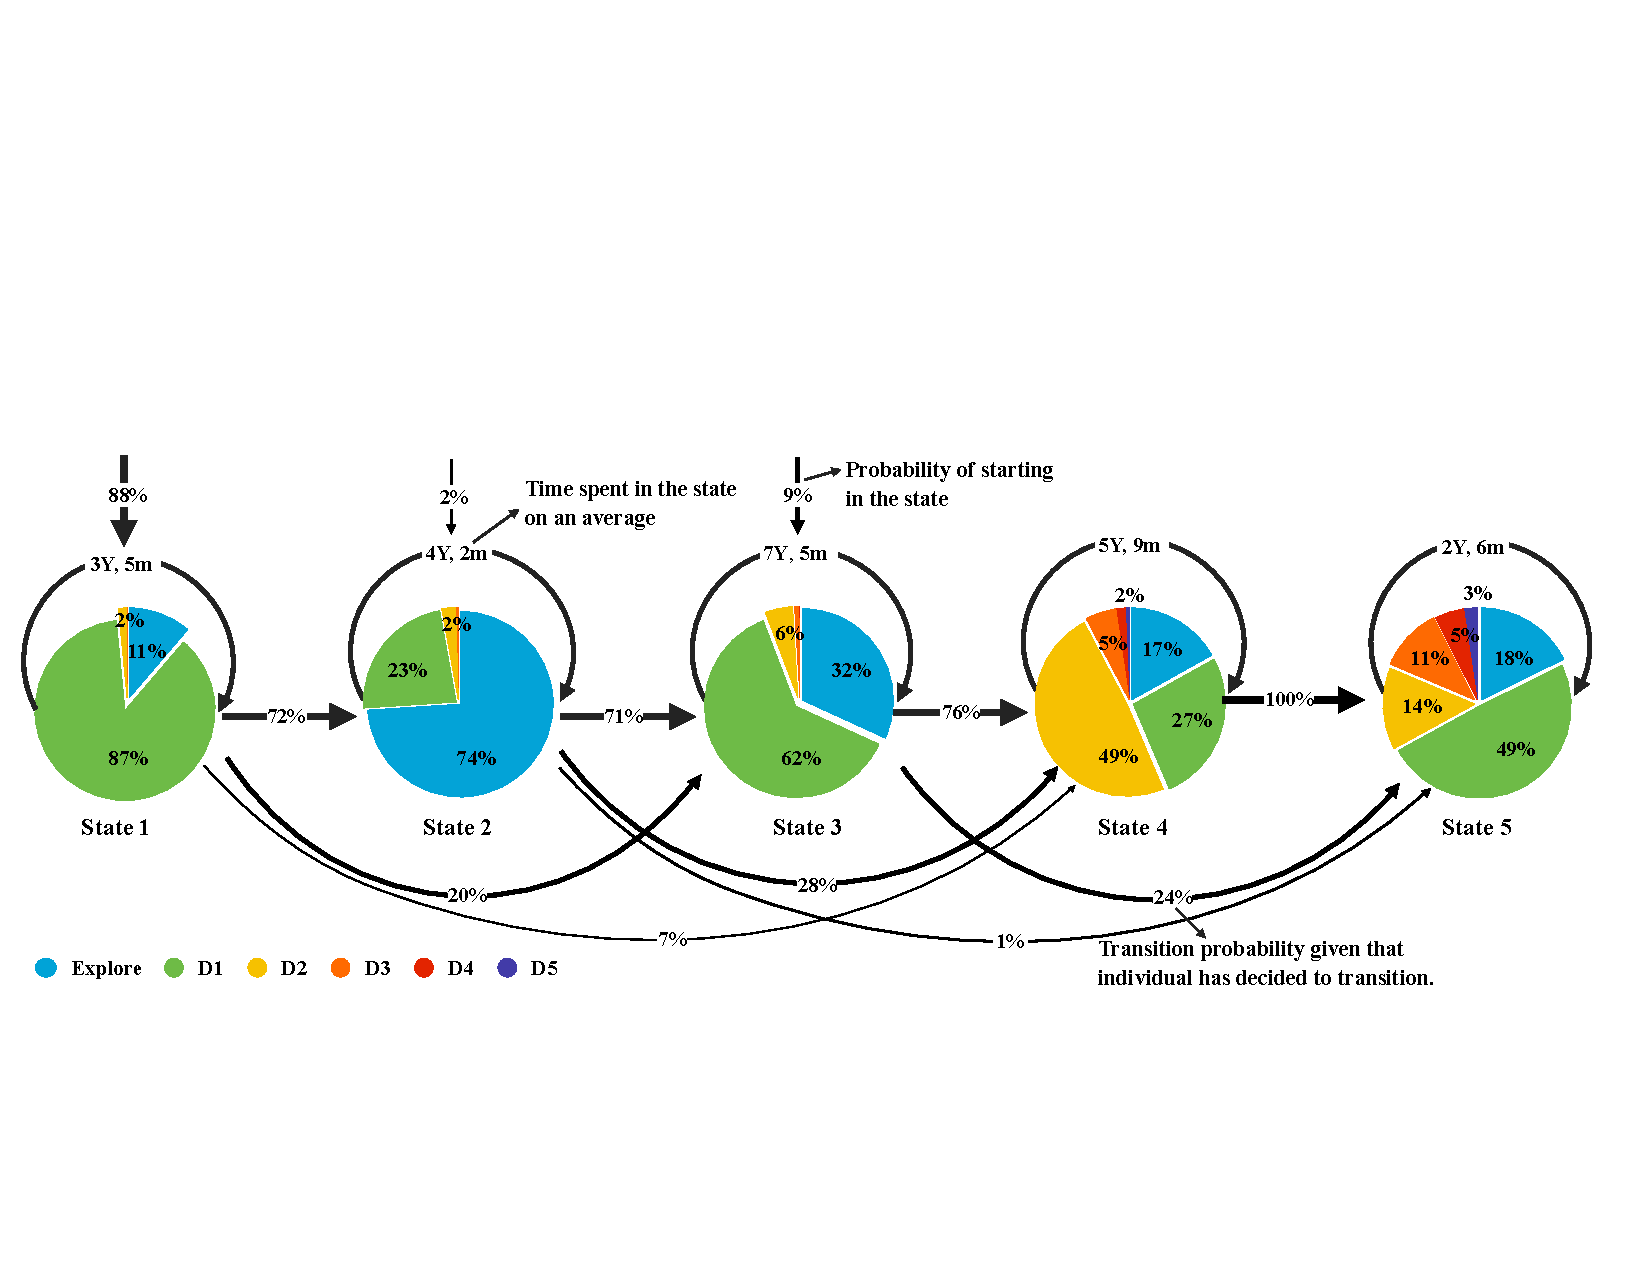
\includegraphics[width=1\linewidth,height=6.4cm]{figures/Cluster4_Self.pdf}
	\end{subfigure}
	\caption{%\small
	\label{fig:acadclusters} Trajectory (state sequence) for \emph{Steady} archetype in the Academic Dataset. Each pie is a \emph{latent state} or \emph{behavioral stage} in the trajectory. It denotes the mean proportion of papers published in each \emph{Area of Interest}'s in the latent state. Each state is also labeled with the average amount of time spent in the state. For example, in this cluster, 87\% of publications in the first 3.5 years are in the author's primary \texttt{AoI} $D_1$ while rest 11\% are in exploring other areas. The arrows on the top of each pie show the prior probability for starting in that state. As we learn a left-to-right G-HMM, an author can transition to its immediate next state or any later latent states. Each transition is labeled with the corresponding conditional transition probability i.e., transition probability given that the user has decided to transition. The arrows thickness is proportional to its weight. Authors in this cluster exhibit \emph{steady} research interest in their primary \texttt{AoI} $D_1$. Some authors start contributing dominantly in their secondary \texttt{AoI}, $D_2$ in State 4. Though, they return to spending around half of their effort in $D_1$ in State 5.
	}
	\label{fig:academic}
\end{figure*}

\begin{table}[!h]
	\centering
	\begin{tabular}{p{40mm} p{25mm} p{25mm} p{25mm} p{25mm}@{}}
		\toprule
		{Behavioral Stage}  & {Steady} & {Diverse} & {Evolving} & {Diffuse} \\
		\midrule
		Stage \textbf{1}& \{3Y, 5m\} \newline $\mathbf{D_1}$ (87\%) \newline Ex (11\%) &
		\{3Y, 3m\} \newline $\mathbf{D_1}$ (88\%)\newline Ex (11\%)&
		\{2Y, 9m\} \newline $\mathbf{D_1}$ (72\%)\newline Ex (24\%) &
		\{2Y, 7m\} \newline $\mathbf{D_1}$(76\%) \newline Ex (22\%) \\\\
		Stage \textbf{2} &  \{4Y, 2m\} \newline \textbf{Ex} (74\%)\newline ${D_1}$ (23\%) &
		\{2Y, 6m \} \newline \textbf{Ex} (80\%)\newline ${D_1}$ (16\%) &
		\{2Y, 9m \} \newline \textbf{Ex} (83\%)\newline ${D_1}$ (12\%) &
		\{3Y, 7m \} \newline \textbf{Ex} (91\%) \\\\
		Stage \textbf{3} & \{7Y, 5m\} \newline $\mathbf{D_1}$ (62\%) \newline \textbf{Ex} (32\%)  &
		\{5Y, 6m\} \newline $\mathbf{D_1}$ (73\%) \newline Ex (17\%) &
		\{6Y, 2m\} \newline $\mathbf{D_1}$ (33\%) \newline \textbf{Ex} (28\%) \newline $\mathbf{D_2}$ (24\%)&
		\{8Y, 5m\} \newline $\mathbf{D_1}$ (50\%) \newline \textbf{Ex} (39\%) \\\\
		Stage \textbf{4} & \{5Y, 9m\} \newline $\mathbf{D_2}$ (49\%) \newline $\mathbf{D_1}$ (27\%) \newline Ex (17\%) &
		\{5Y, 6m\} \newline $\mathbf{Ex}$ (46\%) \newline ${D_2}$ (20\%) \newline ${D_1}$ (17\%)&
		\{5Y\} \newline $\mathbf{D_2}$ (66\%) \newline $Ex$ (18\%)  &
		\{3Y, 9m\} \newline $\mathbf{D_2}$ (43\%) \newline $\mathbf{Ex}$ (26\%) \\\\
		Stage \textbf{5} & \{2Y, 6m\} \newline $\mathbf{D_1}$ (49\%) \newline {Ex} (18\%) \newline ${D_2}$ (14\%) &
		\{6Y, 3m\} \newline $\mathbf{D_4}$ (29\%) \newline \textbf{Ex} (20\%) \newline ${D_3}$ (14\%) \newline ${D_1}$ (14\%) &
		\{6Y, 5m\} \newline $\mathbf{D_3}$ (43\%) \newline {Ex} (19\%) \newline ${D_2}$ (14\%) &
		\{4Y, 1m\} \newline \textbf{Ex} (74\%) \\
		\bottomrule
	\end{tabular}
	\caption{
	\label{tab:mean} Learned mean vector for each latent state of four archetypes in the Academic Dataset. We list the \emph{Area-of-Interests} (\texttt{AoI}) in sorted order and annotate them with their \% contribution in the state. We only list significant \texttt{AoI} ($>$ 11\%) for each state. Each state is also labeled with its average duration in \{Years (Y), months (m)\}. The labels given to these clusters reflect our interpretation of the user behavior and make disambiguation of the behavior easier in the text.}
\end{table}

\texttt{Commonalities in Archetypes:} Table \ref{tab:mean} summarizes the trajectories (state sequences) learned for the four different archetypes in this dataset. Each archetype is labeled according to our interpretation of the user behavior, looking at the learned mean vector of G-HMM states. We observe that all archetypes exhibit similarities, especially in the first two stages. Across all archetypes, the first \emph{stage} typically spans around $3$ years, and more than 72\% of the published research is in the author's \emph{primary} \texttt{AoI}: $D_1$. As noted before, this is most likely their Ph.D. dissertation area, and hence, the research is more focused. After gaining some research experience, most authors move to the second \emph{stage} where they start exploring other research areas denoted by a marked increase in their \emph{Explore} \texttt{AoI}(more than 74\%). However, in state 3 and beyond, authors from different archetypes follow different trajectories where they differ in how they change their dominant \texttt{AoI} over time while \emph{exploring} other domains \footnote{We observe that all archetypes have similar number of authors (\cref{tab:acadclusterdata}) and similar average number of active publication years.}. Below, we describe each archetype in more detail.

\texttt{Steady}: The first major archetype is of \emph{steady} researchers, who mainly work in \emph{one} \texttt{AoI} (i.e. their $D_1$) throughout their career. Fig \ref{fig:academic} shows the state sequence of this archetype. We can see that most people start in their primary \texttt{AoI}, $D_1$ (state 1), which possibly reflects their Ph.D. education. After graduation, they spend some time \emph{exploring} other areas while continuing to publish in $D_1$ (state 2), but move back to publishing in $D_1$ for a significant portion of their careers, about 7.5 years (state 3). This shift is often again followed by a phase where they start working in another area, $D_2$, while continuing to publish in $D_1$ (state 4). They eventually revert to publishing in $D_1$ (state 5) towards the latter part of their careers. In the last state, they also publish widely in other areas (indicated by almost half of the pie divided between other $D_m$'s), but their main interest remains $D_1$.

For example, Michael Jordan, professor at the University of California, Berkeley exhibits this research trajectory. He is a Machine Learning expert; his primary \texttt{AoI} $D_1$, and has secondary interests in Data Mining, Optimization, and Bioinformatics.
Theory professor at University of Illinois, Urbana-Champaign (UIUC), Jeff Erickson is also assigned to this cluster; he also publishes in his primary \texttt{AoI} $D_1$ (Theory) with auxiliary interests in mathematical optimization.

\texttt{Diverse}: The second archetype consists of researchers with \emph{diverse} research interests as they make significant contributions in multiple $D_m$'s. Similar to \emph{steady} researchers, these researchers research in their primary \texttt{AoI} $D_1$ while \emph{exploring} other domains in the initial $3$ states as shown in Table \ref{tab:mean}. They, then, publish in $D_2$ and $D_1$ while spending half time \emph{exploring} other possible interests (state 4). They evolve to have a strong research presence in all $5$ AoIs (state 5). This behavior suggests that authors of this archetype tend to work in interdisciplinary areas; or possibly projects with a broader scope which gains acceptance by different research communities.
One notable example is Prof. Jiawei Han at UIUC, who started his academic career studying Databases and Data Mining, is also making notable contributions in Machine Learning and Bioinformatics lately.
Another professor who started in Databases, Jaideep Srivastava of the University of Maryland, evolved on to research distributed implementation of databases, and also data mining and AI-related research simultaneously.

\texttt{Evolving}: These researchers have one dominant area of interest (\texttt{AoI}) in each state which \emph{changes} with time. Their dominant  area of interest (\texttt{AoI}) \emph{evolves} from $D_1$ (72\%) in state 1 to $D_2$ (66\%) in state 4 to $D_3$(43\%) in state 5. Even though their \texttt{AoI} shifts across stages, in any given stage, they remain focused on one area and do not publish much in other areas.
James Foley, a professor in Georgia Tech, started in Computer Graphics and later switched to research on user-computer interfaces and recently, User Modeling.
Natural Language Processing (NLP) expert Daniel Jurafsky at Stanford University, also steadily moved from pure NLP based research problems to Speech processing, and later to Machine Learning (ML). Also note, for Jurafsky, this evolution can be attributed to the broader field shift of using sophisticated ML models to solve NLP problems.

\texttt{Diffuse}: Authors of this archetype stay focused in one dominant area in each stage; while in the last stage, their research interests are \emph{diffused}. Authors publish considerably in one dominant area in first 3 stages; $D_1$ (state 1, 3) to $D_2$ (state 4). In the last state, which lasts around four years, the authors are infrequently publishing (less than three papers a year) in new subfields accounting for 74\% of their publications. Hence, these authors have \emph{diffused} research interests after they gain experience.
Gerhard Weikum, professor at MPI Germany started in Databases area made a brief transition to Information Retrieval work and later started publishing in Machine Learning and Data Mining fields too. These area evolutions seem to be natural transitions as they are highly interrelated, which explains contributions in all fields.
Anind Dey, professor at Carnegie Mellon University, initially worked on sensor technology and then switched to Web mining and Human Computing related research problems is also another example of this archetype.

\subsection{Archetype variations across Gender}
\label{sec:discussion}
We now proceed to analyze the variations in the evolution of research interests (or archetypes) between male and female researchers. To this end, we manually annotate gender of all current and emeritus professors in top 50 Computer Science (CS) Universities as reported by U.S. News \& World Report\footnote{\url{bit.ly/usnews-cs}}. We consider only current and emeritus \emph{Full} Professors as they typically have 15 or more years of publication history. This results in a total of 1084 authors in our dataset, 127 of whom are women. ~\Cref{tab:acadclusterdata} shows the distribution across archetypes. We observe similar gender distribution in each archetype with the least number of women academics in \emph{evolving} archetype.

\begin{table}[h]
    \centering
    \begin{tabular}{l r r r r}
        \toprule
             Social Group   & Steady  & Diverse & Evolving & Diffuse \\ \midrule
        Male    Professors (Top-50 US schools) & 247     & 206     & 241    & 263   \\
        Female Professors (Top-50 US schools) & 30     & 32    & 26    & 39  \\
        All authors in the dataset   & 1329    & 1080     & 1107    & 1062   \\ \bottomrule %
    \end{tabular}
    \caption{ \label{tab:acadclusterdata} Statistics for discovered archetypes in relationship to different social groups.}
\end{table}


While researchers from both genders in the same archetype $c$ will traverse the same set of stages, they may differ in \textit{how} they transition $\tau^c$, and at \textit{which} stage they start $\pi^c$. For this analysis, we first run our model on the entire dataset assigning archetypes to each individual. We then estimate separate model parameters for female $\lambda^c_f$ and male $\lambda^c_m$ researchers for each archetype $c$ using the assigned values.

To quantify the difference between two models ($\lambda^c_f, \lambda^c_m$) for archetype $c$, we compute their \emph{likelihood ratio}. Likelihood ratio $R^c_f$ of female researchers in archetype $c$ is:

\begin{equation}
    R^c_f = \exp \left ( \frac{1}{|N^c_f|} {\sum_{i \in {N_f}} \log \frac{ P(X_i | \lambda_f^c)}  {P(X_i | \lambda_m^c)}} \right )
    \label{eq:confusion metric}
\end{equation}

where $N^c_f$ represents all female researchers in $c$-th archetype. The equation simplifies to say that $\displaystyle \log R^c_f$ is the average difference between log-likelihoods of a trajectory of a female researcher generated from their own model with those of male model of the same archetype. Thus, for instance, value of $\displaystyle R^c_f = 2$ denotes that female researchers are twice more likely to be generated by the model of their own gender than of the opposite gender. We compute a similar ratio, $R^c_m$, for men. We also conduct paired-sample t-test \cite{goulden:1949} between the two likelihood values similar to ~\Cref{sec:acad}.

\begin{table}[tbh]
    \centering
    \begin{tabular}{lllll}
        \toprule %
        Gender & Steady & Diverse & Evolving & {Diffuse} \\
        \midrule
        Male   & 2.10***  & 2.63**  & 1.15  & 1.10   \\
        Female & 1.80***  & 1.64**  & 1.60***  & 1.38***    \\
        \bottomrule
    \end{tabular}
    \caption{
    \label{tab:genderclusterdata} Likelihood ratio for academics across genders within an archetype. It measures odds of a researcher being better explained by model for their gender than by model for the other gender.\\ $* = p < .05, ** = p< .01, *{*}* = p < .001$}
\end{table}

\Cref{tab:genderclusterdata} shows the likelihood ratio with their $p$-values. Since most of the values are statistically significant, all researchers are better explained by the model for their gender, than by the model for the opposite gender. Male researchers are distinct for the steady and diverse archetypes, but not for the evolving and diffuse archetypes. For women, on average, the difference is larger, with the strongest difference seen for the steady, diverse, and evolving archetypes.

\begin{figure*}[tbh]
        \centering
        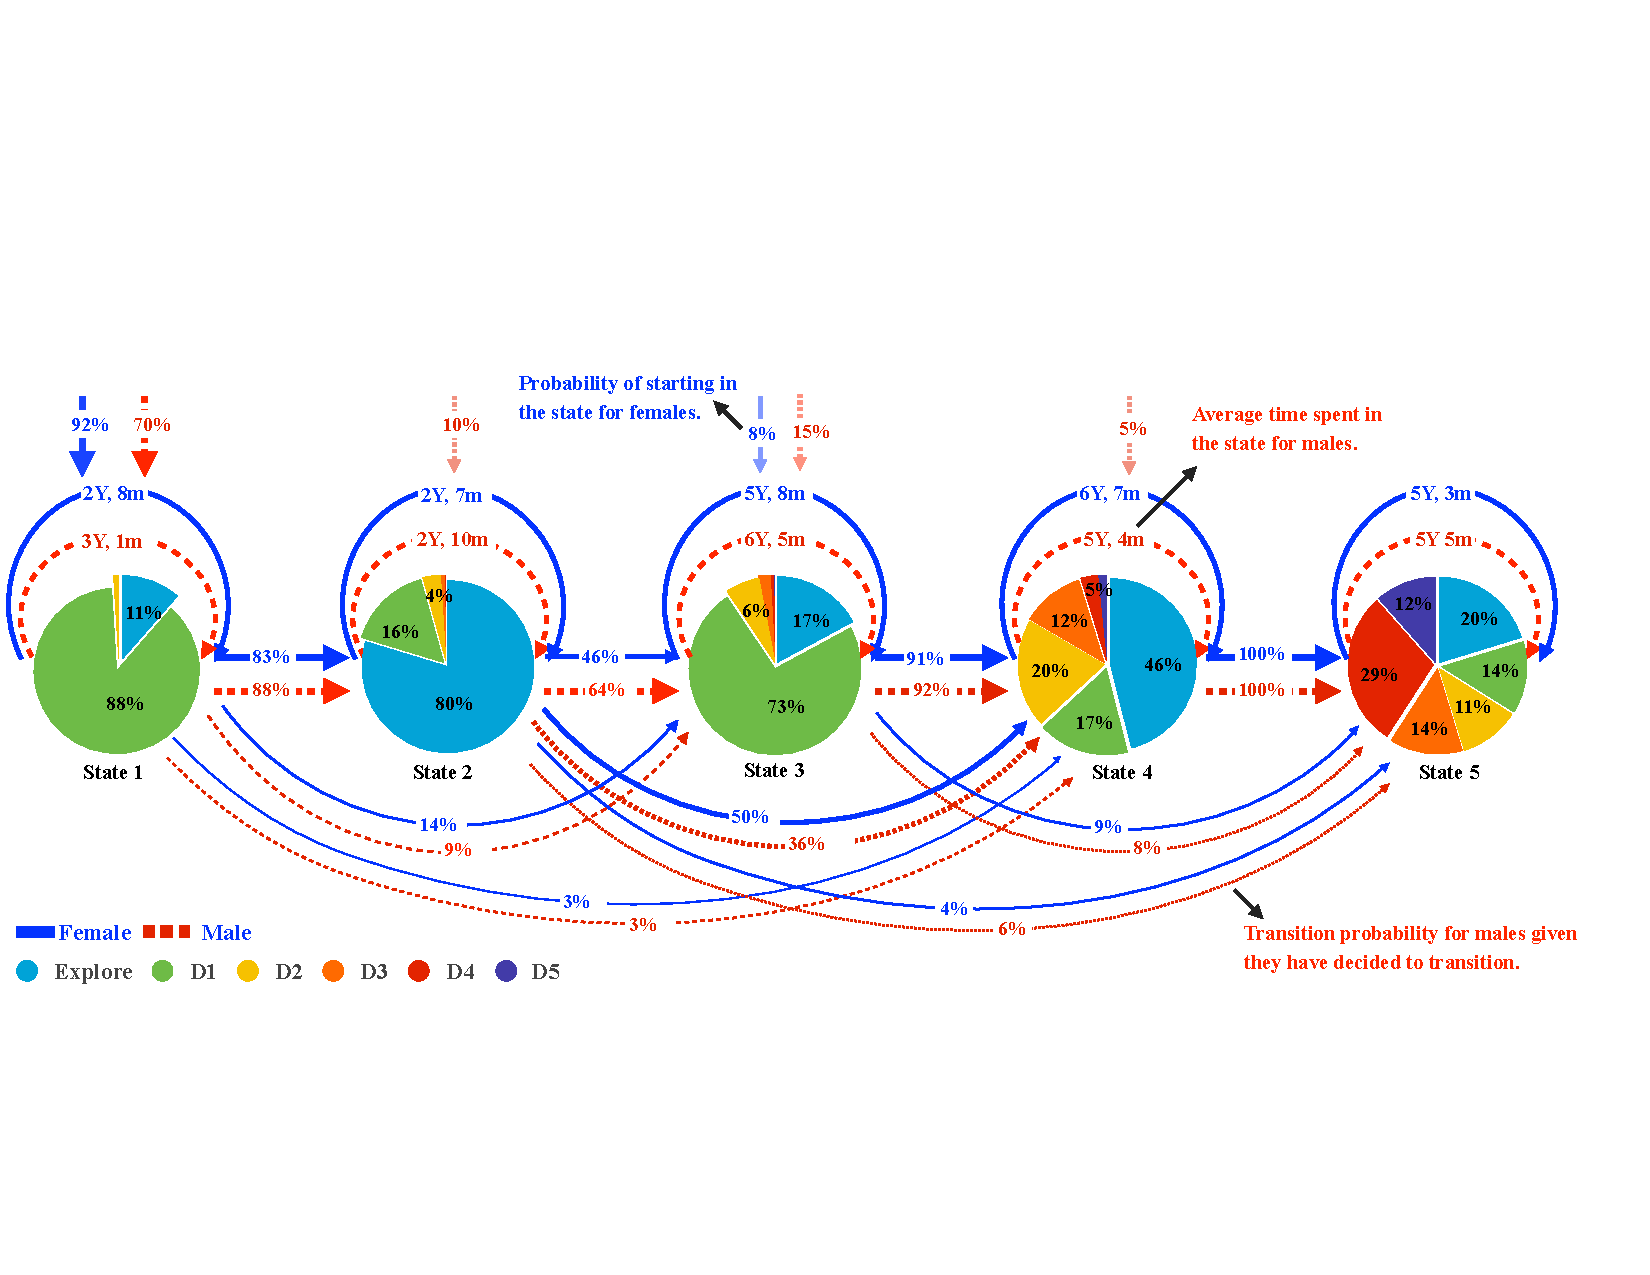
\includegraphics[width=1\linewidth,height=7cm]{figures/Cluster3_both_Self.pdf}
    \caption{
    \label{fig:genderacadclusters} Gender wise representation of trajectory for researchers belonging to the \emph{diverse} archetype in the Academic Dataset. The transitions in blue denote transition probabilities of female professors in the archetype while those in red represents probabilities for their male counterparts. Men start their career from later evolved stages while women make long term state transitions.}
    \label{fig:academic_gender}
\end{figure*}

For the sake of brevity, we examine gender difference in only the \emph{diverse} archetype in some detail. ~\Cref{fig:academic_gender} shows three interesting variations. First, we observe that women are much more likely to start in state 1 (92\%), with a dominant area of interest ($D_1$) than in any other state. In contrast, men start in states 1, 2, 3, and 4, with only 70\% starting in state 1. Both men and women skip stages, but women are more likely to skip a stage than men. For example, 50\% of women skip stage 3, while only 36\% of men do. Longer skips of two stages are rarer, and both women and men make these long skips at the same rate. Finally, there are clear differences between mid-career men and women (states 3, 4): women spend more time \emph{exploring} mid-career (state 4) than men, and mid-career men spend more time in their starting area of interest ($D_1$, state 3) than women.

\subsection{Grant income variability across Archetypes \& gender within an Archetype}
\label{sec:grant}
We next examine the relationship between variation in the academic trajectories and gender to research grants awarded at different stages of an academic career. We extract historical information of grants from the National Science Foundation, a large federal funding agency for Science \& Engineering in the United States \footnote{\url{bit.ly/nsfgrants}}. We consider grants with Principal Investigators (PI) from the same subset of CS professors in top-50 US universities as in~\Cref{sec:discussion}. We collect information for 1062 professors and manually disambiguate names and identify gender by cross-validating with the researcher's webpage.
Then, we compute the average grant money awarded to a researcher, at each stage in their trajectory. ~\Cref{fig:grantanalysis}, which shows letter-value plots of average grant size awarded as PI's, broken down by archetypes (steady, diverse, evolving or diffuse), stage within an archetype and gender, summarizes our findings.

\begin{figure*}[tbh]
    \centering
    \begin{subfigure}{0.5\linewidth}
        \centering
        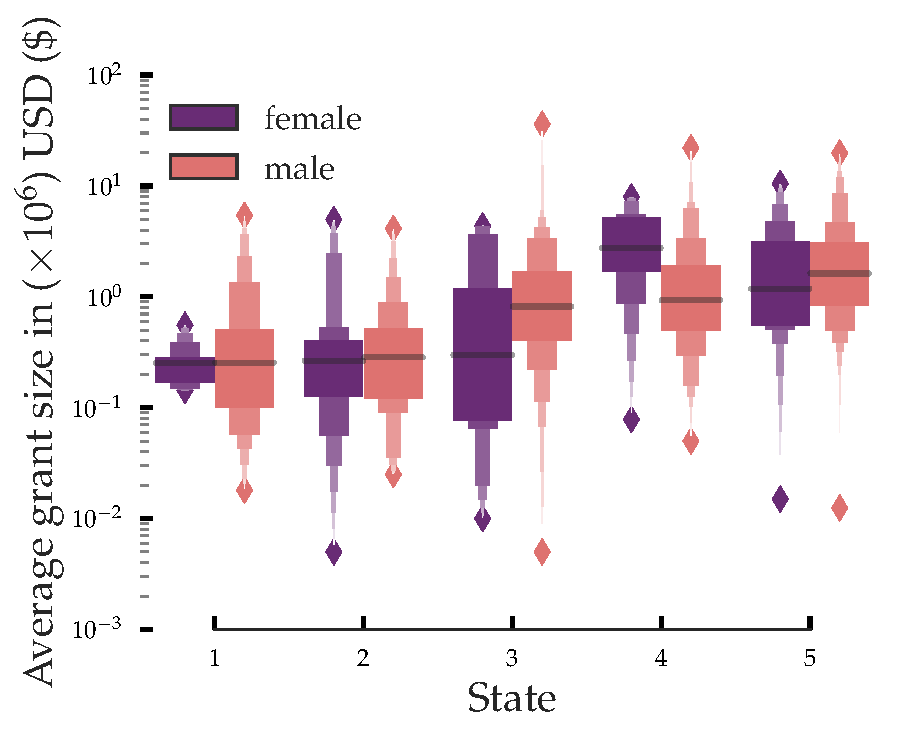
\includegraphics[width=0.8\linewidth,height=5cm]{figures/Cluster_4_PI_grant.pdf}
        \caption{Steady Researchers}
    \end{subfigure}%
    \begin{subfigure}{0.5\linewidth}
        \centering
        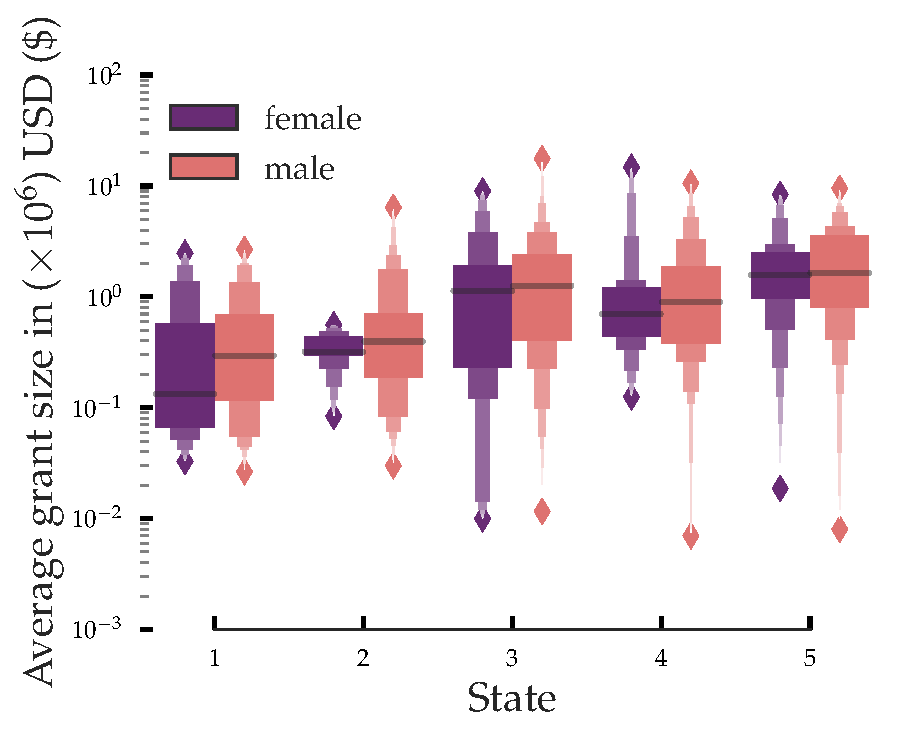
\includegraphics[width=0.8\linewidth,height=5cm]{figures/Cluster_3_PI_grant.pdf}
        \caption{Diverse Researchers}
    \end{subfigure}
    \begin{subfigure}{0.5\textwidth}
        \centering
        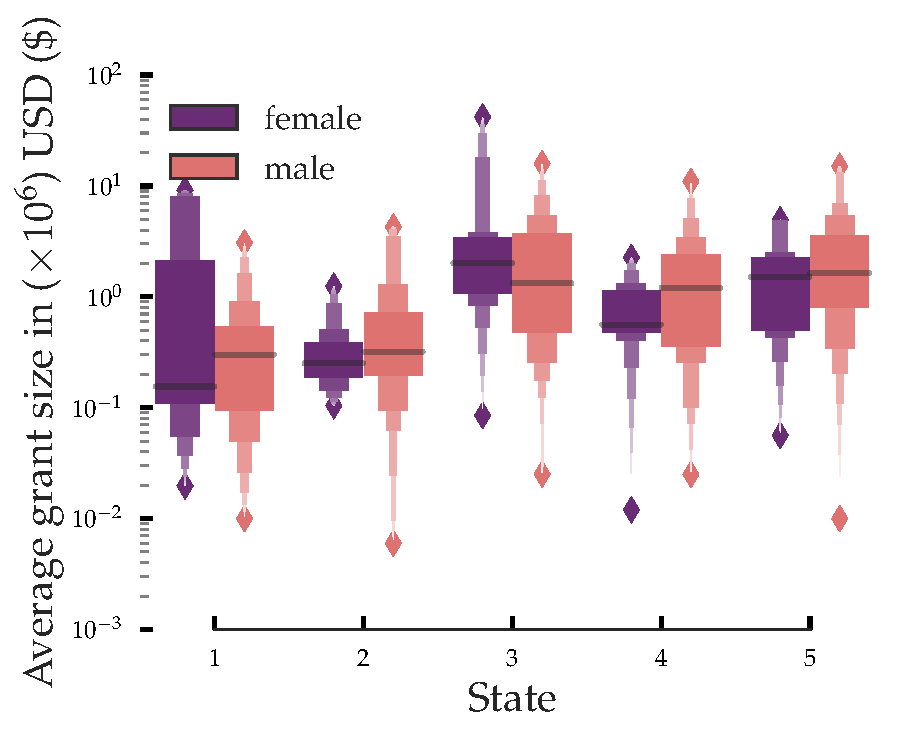
\includegraphics[width=0.8\linewidth,height=5cm]{figures/Cluster_1_PI_grant.pdf}
        \caption{Evolving Researchers}
    \end{subfigure}%
    \begin{subfigure}{0.5\textwidth}
        \centering
        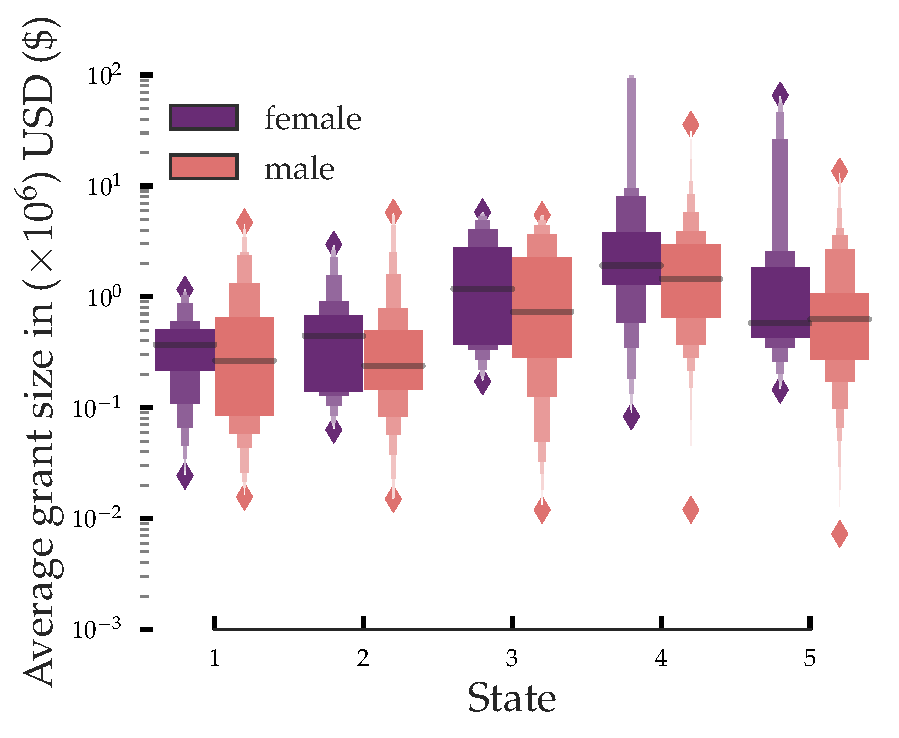
\includegraphics[width=0.8\linewidth,height=5cm]{figures/Cluster_2_PI_grant.pdf}
        \caption{Diffusive Researchers}
    \end{subfigure}
    \caption{\small \label{fig:grantanalysis} Letter value plots of total grant money awarded by NSF when author is a PI in each stage. In general, Professors get more grant money as they gain experience. Regardless of archetypes, grant income in state 3 is significantly higher from state 2 (p< .01). There are also significant differences across genders within a state of an archetype. For instance, for Evolving archetype, male professors get significantly more income than female professors in state 4 (p < .01).}
\end{figure*}

\begin{table}[tbh]
\centering
\begin{tabular}{ll}
\toprule
Archetype (H-test) &  State Pair (t-test)  \\
\midrule
\multirow{2}{*}{Steady***}    & State 2 vs 3**    \\
                     & State 4 vs 5*    \\
\hline
\multirow{2}{*}{Diverse***}   & State 2 vs 3*** \\
                                    & State 4 vs 5*    \\ \hline
\multirow{3}{*}{Evolving***}  & State 2 vs 3***   \\
                         & State 3 vs 4*    \\
                        & State 4 vs 5**    \\ \hline
\multirow{1}{*}{Diffuse***}   & State 2 vs 3***     \\
\bottomrule
\end{tabular}
\caption{ \small Statistical significance tests for the differences in grant money across latent states within an archetype. Shown are only those tests that are statistically significant. H-test \cite{Kruskal:1952} confirms that at least one state is different from another state of the archetype; t-test \cite{Welch:1947} was then conducted between each consecutive states within the archetype to determine the differing states. $* = p < .1, ** = p< .01, *{*}* = p < .001$ }
\label{tab:statstate}
\end{table}


Additionally, we conducted Kruskal-Wallis H-test~\cite{Kruskal:1952} to establish the statistical significance of differences in grant money across latent states within an archetype. This test affirms that at least one latent state is different from another latent state within an archetype \footnote{ We also conducted H-test for the difference in average grant income across archetypes for the same state. However, we did not find any significant differences. \Cref{fig:grantanalysis} can easily verify this lack of difference. }. We then conducted Welch's t-test~\cite{Welch:1947} between consecutive states to find the exact pair of states which are significantly different. We only tested with consecutive latent states as we are only interested in grant income changes as the author progresses through stages. ~\Cref{tab:statstate} reports the state pairs for each archetype that are statistically different. In the rest of this section, we describe these results in detail.

Regardless of archetypes, we observe that in general authors tend to receive more grant money as they gain experience in~\Cref{fig:grantanalysis}. On average, across archetypes and gender, PI's receive in state 5, four times the amount of grant money than state 1 ($p < .001$). Also for researchers across archetypes and across genders, we notice an uptick in grant income in state 3 from state 2 ($p < .01$ - ~\Cref{tab:statstate}). Let us qualitatively examine the \emph{steady} researchers in detail, by comparing~\Cref{fig:grantanalysis} with~\Cref{fig:acadclusters}. State 2 in~\Cref{fig:acadclusters} shows the researchers exploring different topics, whereas, in state 3, they are spending a significant part of their time on their main domain $D_1$. Also, notice that 36\% of the researchers never visit state 2 - 27\% skip state 2, and 9\% of the researchers start in state 3. Since state 1 typically represents the time spent by the researchers in their Ph.D., and with 74\% time spent in an explore stage in state 2, it is not surprising that we see limited grant income in their first two states. State 3, perhaps reflects a sustained focus on their domain $D_1$, and this pays off in terms of grant income. Similar qualitative arguments follow for the other archetypes.


\begin{table}%[tbh]
\centering
\begin{tabular}{ll}
\toprule
Archetype & Latent State (t-test) \\
\midrule
\multirow{2}{*}{Steady}   & State 1* \\
& State 4*  \\ \hline
Diverse   &  State 2*  \\ \hline
\multirow{2}{*}{Evolving}  & State 4** \\
& State 5*    \\  \hline
Diffuse & {Not significant}  \\
\bottomrule %\hline
\end{tabular}
\caption{ \small
\label{tab:statgender}Statistical significance tests \cite{Welch:1947} for the differences in grant money across gender in each state within an archetype. Shown are only those tests that are statistically significant. \\ $* = p < .1, ** = p< .05, *{*}* = p < .001$}
\end{table}

However, the grant trajectories over states is different for each archetype ($p < .001$). Let us examine statistically different state pairs from ~\Cref{tab:statstate} in ~\Cref{fig:grantanalysis}. Steady researchers see a big uptick in their grant income in state 3 ($p < .01$) and a dip in state 5 ($p < .1$), perhaps due to switching back to their primary research area. The grant income for diverse researchers (who have more than one dominant area) increases steadily over states($p < .05$). For evolving researchers (who change their dominant area), the grant income rises (state 3, $p < .001$), falls (state 4, $p < .05$) and rises (state 5, $p < .1$), reflecting a degree of unpredictability accompanying \emph{changing area of interest}. Diffuse researchers see an increase in funding in state 3 ($p < .001$) with similar grant income in subsequent states.

To determine differences in grant income across gender, we further conducted t-test \cite{Welch:1947} between grant distributions of female and male professors in each state within an archetype. ~\Cref{tab:statgender} reports significantly different states within each archetype. We again examine these statistically different states from ~\Cref{tab:statgender} in ~\Cref{fig:grantanalysis}. Evolving women receive significantly \emph{lower} income than evolving men when they \emph{switch to new areas} in state 4 and 5 ($p < .05$). On the other hand, in our dataset, steady women receive significantly \emph{higher} grant income than steady men when they \emph{switch areas} in state 4 ($p < .05$). In general, we observe that men show greater grant income variability than do women. The variability is statistically significant ($p < .05$) during early career in state 1 and 2 for Steady and Diverse researchers respectively. We do not observe significant differences in grant income of male and female Diffusive researchers.


\subsection{StackOverflow Archetypes}
\label{sec:stack}
\begin{table}[!h]
	\centering
	\begin{tabular}{p{30mm} p{25mm} p{25mm} p{25mm} p{25mm}@{}}
		\toprule
		  & Experts & Seekers & Enthusiasts & Facilitators \\
		\midrule
		State 1& \{14.4S\} \newline $\mathbf{A}$ (68\%) \newline C (19\%) &
		\{3.7S\} \newline $\mathbf{Q}$ (69\%)\newline C (19\%)&
		\{12.6S\} \newline $\mathbf{C}$ (42\%)\newline \textbf{Q} (39\%) &
		\{15.4S\} \newline $\mathbf{Q}$(50\%) \newline C (32\%) \\
		State 2 &  \{17.8S\} \newline \textbf{C} (60\%)\newline ${A}$ (25\%) &
		\{8.4S\} \newline \textbf{C} (51\%)\newline ${Q}$ (33\%) &
		\{9.5S\} \newline \textbf{A} (49\%)\newline ${C}$ (32\%) \newline ${E}$ (12\%)&
		\{26.4S\} \newline \textbf{C} (44\%) \newline ${A}$ (28\%) \newline ${E}$ (22\%)\\
		State 3 & \{9S\} \newline $\mathbf{A}$ (87\%)  &
		\{2.2S\} \newline $\mathbf{A}$ (84\%) &
		\{3.7S\} \newline $\mathbf{E}$ (82\%) &
		\{8.4S\} \newline $\mathbf{A}$ (87\%)  \\
		State 4 & \{12.3S\} \newline $\mathbf{C}$ (82\%)  &
		\{5.3S\} \newline $\mathbf{C}$ (72\%) \newline ${Q}$ (15\%) &
		\{9S\} \newline $\mathbf{C}$ (75\%) \newline $A$ (10\%)  &
		\{24.2S\} \newline $\mathbf{C}$ (68\%) \newline $\mathbf{A}$ (14\%) \newline $E$ (13\%) \\
		State 5 & \{5S\} \newline $\mathbf{E}$ (45\%) \newline {C} (28\%) \newline ${A}$ (21\%) &
		\{3.7S\} \newline $\mathbf{Q}$ (85\%) &
		\{10.5S\} \newline $\mathbf{Q}$ (40\%) \newline {C} (33\%) \newline ${E}$ (16\%) &
		\{14.3S\} \newline \textbf{E} (63\%) \newline ${C}$ (22\%) \\
		State 6 & \{11S\} \newline $\mathbf{C}$ (48\%) \newline {A} (38\%)  &
		\{7.7S\} \newline $\mathbf{C}$ (55\%) \newline \textbf{Q} (23\%) \newline ${E}$ (11\%) &
		\{5S\} \newline $\mathbf{A}$ (61\%) \newline {C} (23\%) \newline ${E}$ (11\%) &
		\{21S\} \newline \textbf{C} (57\%) \newline ${E}$ (24\%) \newline ${A}$ (13\%) \\
		\bottomrule
	\end{tabular}
	\caption{\label{tab:stackexchangemean} Learned mean vector for each state for four archetypes in the Stack Overflow Dataset. We list the \emph{activities} in sorted order and annotate them with their \% contribution in the state. We list main activities ($>$ 11\%) for each state. Each state is also labeled with it's average number of sessions. The labels reflect our own interpretation of the user behavior.}
\end{table}

We now describe archetypes learned for the Stack Overflow data. Table \ref{tab:stackexchangemean} depicts the latent states for all archetypes. We label the 4 archetypes discovered as \emph{Expert}, \emph{Seekers}, \emph{Enthusiasts} and \emph{Facilitators}. Posting Comments is the most frequent activity in all archetypes as it is a very low cost activity. Moderator actions and Edits are least favored activities by Stack Overflow users. Most of the users spend initial sessions for \emph{posting questions} (state 1) and significant proportion of their later sessions in \emph{posting answers or comments} (state 6).

\texttt{Experts} users join the community to answer queries or post clarifications or edit answers (state 1-6). They spend at least 68\% of their sessions in \emph{posting answers} (state 1 \& 3). They rarely ask questions of their own. In
communities like Stack Overflow, it is vital to have a dedicated group of experts answering queries for it to be sustainable.

\texttt{Information Seekers}
join the community for getting answer to their queries accounting for 69\% of activities per session (state 1). They briefly start contributing by posting answers to the community (state 3) but they end up again in \emph{commenting} (state 6) or \emph{asking questions} (state 5).

\texttt{Enthusiasts} start by asking questions and posting comments (state 1). They, then, start answering questions and commenting on other answers (state 2). They briefly stay (4 sessions) in edit state (state 3) but end up migrating to either commenting again (state 4) or asking questions and commenting (state 5). We denote them as \emph{Enthusiasts} as they use the platform to post questions while simultaneously answering queries from their acquired knowledge.

\texttt{Facilitators} join for information seeking (state 1) but start posting answers, clarifying and editing in state \emph{2-3}. However, later on they take a more subdued approach and only post comments. The reason for this decreased interest is hard to gauge but identifying these users and retaining their interest could be important to sustain the community.


In summary, we identify four dominant archetypes for researchers: steady, diverse, evolving, and diffuse. We observe differences in the evolution of male and female researchers within the same archetype. When we examine the diverse archetype in detail, we observe that women and men differ in where they start, rate of transition, and time spent in mid-career. The differences in grant income are salient across states within an archetype. In general, grant income increases with experience. We also observe differences across genders within a stage of an archetype mostly accompanied by an area switch. Finally, we also identified dominant archetypes for StackOverflow community: experts, information seekers, enthusiasts and facilitators.

\section{Quantitative Experiments}
\label{sec:experiments}
In this section, we evaluate our model on two different tasks, Future Prediction and Perplexity. We describe the baselines in Section~\ref{sec:baseline} and report results in Section~\ref{sec:tasks}.
\subsection{Baselines}
\label{sec:baseline}
\textbf{Distance G-HMM}: Our first baseline uses the G-HMM clustering model as defined in \cite{HMM2014}. In this baseline, we learn a G-HMM for each user and then cluster the models using distance metric $\delta$, the symmetric KL divergence ($d_{kl}$) between two G-HMMs~\citep{rainier}.
\begin{align}
    \label{eq:KL}
    d_{kl} (\lambda^p, \lambda^q) = \frac{1}{N_p} \sum_{i \in N_p} log \frac{P(X_i | \lambda^p)} {P(X_i | \lambda^q)},
\end{align}

We use k-medoids clustering; since this method does not give a representative model for each cluster, we additionally learn a G-HMM per cluster.
For a fair comparison, we set $k$, the number of clusters to be the same as our model.

\textbf{Vector Autoregressive Model (VAR)}: VAR models are used to model multivariate time series data \cite{Ltkepohl:2007}. It assumes that each variable in the vector is a linear function of its own past values as well as other variables. For each user sequence $\mathbf{X_i}$, $j$th session is modeled as,
\begin{align}
  \vec{X}_{ij} = A_1 \vec{X}_{ij-1} + \ldots + A_p \vec{X}_{ij-p} + u_j
\end{align}
where $A_i$ is \emph{M} X \emph{M} matrix, $u_j \sim \mathcal{N}(0,\,\Sigma_{u}) $ and we set $p=1$ as in first-order Markov models.

\textbf{No Evolution}: In this baseline, we assume that individuals \emph{do not evolve} in their lifespan. This baseline is a simplified version of our model. It assumes that there are different archetypes but that each archetype has only one state. Hence, all sessions of a sequence are generated from a single multivariate Gaussian.

Prior work on activity sequence prediction baselines ~\citep{Yang:2014, Knab2003} deals with discrete data. However, as we represent each session as a continuous vector, these approaches are not directly comparable and adapting them to our problem is nontrivial.

\subsection{Tasks}
\label{sec:tasks}
\textbf{Future Activity Prediction}:
In this task, we predict the future behavior of an individual given her history. We assign the first $90\%$ sessions of each sequence for training and predict the behavior in future sessions (the remaining $10\%$ of the sequence). We first use all the training sessions to learn the parameters of our model. Then, for each sequence, we run the Viterbi algorithm to decode the state assignment of its test sessions, \emph{$t^\prime_i$}. The test sessions of the $i$-th user will have same archetype assignment $c_i$ determined in the training session for that user.

We compute Jensen-Shannon($d_{js}$) divergence between the mean $\mu^{c_{ij}}$ of the assigned state $Y_{ij}$ and the observed vector $X_{ij}$. $d_{js}$ is a symmetric K-L divergence between two vectors. We report the average $\bar{\Delta}$ over all test sessions:

\begin{align}
    \label{eq:pred}
    \bar{\Delta} &= \frac{1}{\textit{$|T|$}} \sum_{i \in N, j \in t^\prime_i} d_{js}(\mu^{c_{ij}}, X_{ij}), \\
    d_{js}(\mu^{c_{ij}}, X_{ij}) & = \frac{1}{2}d_{kl}(\mu^{c_{ij}}, p) + \frac{1}{2}d_{kl}(X_{ij}, p),
\end{align}

where, $p = \frac{1}{2}(\mu^{c_{ij}} + X_{ij})$ and $d_{kl}$ measures KL divergence distance. For VAR, we use the model learnt on training sessions of  user $i$ to make prediction for her future sessions.

Table \ref{tab:futurepred} shows our results on this task.
Our model outperforms the baselines for all Stack Exchange datasets with an average improvement of about 32\% and 24\% on the Academic dataset.
Hence, learning archetypes can also help us to accurately predict an individual's future behavior in the social network.

\begin{table}[tbh]
	\centering
\sisetup{
  round-mode = places,
round-precision = 2
}
		\begin{tabular}{lSSSSS} \toprule
			Dataset                & {Our Model}& {VAR}& {\shortstack{Distance \\ G-HMM}} & {\shortstack{No \\ Evolution}} \\ \midrule
			Academic               & 0.2189  &  0.31    &   0.4151  &  0.2941    \\
			{StackOverflow}       & 0.2289  &   0.3577  & NA  &  0.3715     \\
			{English}              & 0.187 & 0.29 &  0.26      & 0.31 \\
			Money                  & 0.186 & 0.52 &  0.32      & 0.32  \\
			Movies                 & 0.23  & 0.35 &  0.3502    & 0.37 \\
			CrossValidated         & 0.21  & 0.38 &  0.3260    & 0.35  \\
			Travel                 & 0.19  & 0.30 &  0.2547    & 0.29  \\
			Law                    & 0.19  & 0.26 &  0.33      & 0.27  \\ \bottomrule
		\end{tabular}
	\caption{\label{tab:futurepred} Average Jensen-Shannon divergence of future sessions using 90-10\% split of each user sequence. Lower values are better. Distance HMM did not converge on StackOverflow dataset.
   }
\end{table}

\textbf{Perplexity}
Perplexity measures how surprised the model is on observing an unseen user sequence. A lower value of perplexity indicates low surprise and hence a better model.

\begin{equation}
    P_x = - \frac{1}{ \textit{$|T|$} } \sum_{i \in T }  \max_{c \in C}  \left (\log P(\mathbf{X_i^T} | \lambda^{c}) \right )
\end{equation}
where, $\mathbf{X_i^T}$ represents a test sequence in Test Set \emph{T}, and $\lambda_c$ represents the parameters of the G-HMM corresponding to the $c$-th archetype. We assign $\mathbf{X_i^T}$ to the archetype \emph{c} with maximum likelihood. Perplexity is then computed as the average likelihood of all test sequences. In general, $P(\mathbf{X_i^T} | \lambda^{c}))$ is bound between [0,1] but as we model continuous data with multivariate Gaussian distribution, probability is computed as a density function and can be $>1$.

Table \ref{tab:perplexity} reports average perplexity after five-fold cross-validation. Note that for this experiment, the model predicts the entire trajectory of a new user. We could not use the regression baseline (VAR) as it is not a generative model and can not predict an entirely new sequence.
Our model beats best performing baseline by 149\% on Academic and by around 25\% on average for StackExchange communities.
Hence, our model also effectively predicts the behavior of future individuals joining the social network.
Note that our model gives negative perplexity values i.e., negative log values. It indicates that the likelihood is more than one due to the Gaussian kernel, as mentioned earlier.

\begin{table}[tbh]
    \centering
    \sisetup{
        round-mode = places,
        round-precision = 2,
    }
        \begin{tabular}{lSSSS}
            \toprule
            Dataset         & {Our Model}     & {\shortstack{Distance \\ G-HMM}} & {\shortstack{No \\ Evolution}}  \\ \midrule
            Academic        & -18.37  & 37.73  & 100.79       \\
            StackOverflow   & 487.68  & NA           & 678.62   \\
            English          & 306.38  & 559.6459   & 471.137  \\
            Money           & 415.853 & 557.686  & 570.509   \\
            Movies          & 596.10  & 724.15   & 743.73    \\
            CrossValidated  & 398.442 & 514.7365  & 554.313   \\
            Travel          & 494.061 & 645.6434  & 666.966  \\
            Law             & 368.894 & 508.077  & 482.267 \\
        \bottomrule
        \end{tabular}
    \caption{
    \label{tab:perplexity} Average Perplexity on unseen user sequences after 5-fold cross validation. Lower values are better. Note negative log values are because of continuous densities.
  }
\end{table}

\textbf{Discussion:} For future prediction, our model performs better than the VAR model. It shows that modeling cluster of sequences gives a better estimate than modeling each user sequence separately. Also, if we assume no evolution and just cluster users according to their behavior i.e., \emph{No Evolution} model, we obtain worse results indicating that individuals behavior does not stay constant over time.
Our model also outperforms the similarity distance-based clustering method: Distance G-HMM \citep{HMM2014}, which is also the strongest baseline. It first estimates the G-HMM model for each user sequence and then clusters these models. Estimating model for each sequence can be noisy, especially if the user sequence has a short length. Instead, when we jointly learn G-HMM model parameters and cluster sequences, we learn a better approximation.

\textbf{Full vs. Left-Right Transition Matrix}: We also test our model with unconstrained full transition matrix where users can jump from one state to any other state in the HMM. We obtain slightly better results with this model for the future prediction task. This improvement can be due to more degrees of freedom, but then, it is also computationally expensive to learn. However, our model gives comparable results with much fewer parameters. Also, with full transition matrix, learned states are not interpretable in the context of evolution. As \citet{Yang:2014} and \citet{Knab2003} also noted, forward state transitions accurately models the natural progression of evolution, we thus chose to work with a forward transition matrix.

\section{Conclusion}
\label{sec:conclusion}
In this chapter, we aimed to discover the archetypical research behavior of Academics. The observation that despite surface variation in terms of sub-fields, the change in behavior exhibits regularities, motivated our research. We introduced a novel Gaussian Hidden Markov Model Cluster (G-HMM) to identify archetypes and evolutionary patterns within each archetype. We chose to work with G-HMM's since they allow for: variations in trajectories and different evolutionary rates; constrain how individuals can evolve; are interpretable.

We identified four distinct archetypes of computer scientists: steady, diverse, evolving, and diffuse and showed examples of computer scientists from different sub-fields that share the same archetype. We analyzed full professors from the top 50 CS departments to understand gender differences within archetypes.
Women and men differ within an archetype (e.g., diverse) in where they start, rate of transition and research interests during mid-career. We further analyzed grant income of these professors to understand the effect of gender and archetype on income. The differences in income are salient across states within an archetype rather than across archetypes. There also exist significant differences across genders within a state of an archetype. We observed that most of the grant income variability is accompanied by a shift in the dominant research area of the academic. In light of our findings, we propose the funding agencies to be cautious of these differences when deciding on grant applications submitted by researchers venturing into new areas.

To the best of our knowledge, we are the first one to provide a principled framework to model and identify interpretable individual trajectories in academia. Our model can be easily used to identify trajectory in other domains like medicine, physics, and business. Further work on the comparison of research trajectories from the stem and non-stem fields could be an exciting research direction.

For StackOverflow, discovered archetypes could be labeled as: \emph{Experts}, \emph{Seekers}, \emph{Enthusiasts} and \emph{Facilitators}. We showed strong quantitative results with competing baselines for future activity prediction and perplexity.



\chapter{Understanding user latent behavioral characteristics}

\label{chap:reliability}
User behavior is primarily represented using discrete actions like items purchased in the platform, actions performed in the social network or question/answers posted in a CQA forum. However, there is abundant information available in the form of textual content associated with most of these user actions, such as review text or answer text. Analysis of the textual content associated with these actions can provide an in-depth understanding of user preferences.
To this end, in this chapter, we estimate latent user behavior--aspect-based reliability by exploiting the semantic similarity between user provided answers and questions. This latent reliability is in turn used to infer trustworthiness of answers in a CQA forum
\cite{crowdqm} \footnote{This is a joint work with Alex Morales. I was responsible for the conceptualization, experiments and writing. He took care of the idea conceptualization, data collection, model implementation and writing.}.
\section{Overview}
\label{crowdsec:intro}

Users are increasingly turning to community discussion forums to solicit domain expertise, such as querying about inscrutable political events on history forums or posting a health-related issue to seek medical suggestions or diagnosis.
While these forums may be useful, due to almost no regulations on post requirements or user background, most responses contain conflicting and unreliable information~\cite{li2017crowdsourced}. This misinformation could lead to severe consequences, especially in health-related forums, that outweigh the positive benefits of these communities. Currently, most of the current forums either employ moderators to curate the content or use community voting. However, both of these methods are not scalable \cite{gilbert2013widespread}. This creates a dire need for an automated mechanism to estimate the trustworthiness of the responses in the online forums.

In general, the answers written by reliable users tend to be more trustworthy, while the users who have written trustworthy answers are more likely to be reliable. This mutual reinforcement, also referred as the truth discovery principle, is leveraged by previous works that attempt to learn information trustworthiness in the presence of noisy information sources with promising results~\cite{Zhao:2012,Yin:2007,Galland:2010,Dong:2009}. This data-driven principle particularly works for community forums as they tend to be of large scale and exhibit redundancy in the posts and comments.

Community discussion forums encompass various topics, or aspects. A significant deficiency of previous work is the lack of aspect-level modeling of a user's reliability.
This heterogeneity is especially true for discussion forums, like Reddit, with communities catering to broad themes; while within each community, questions span a diverse range of sub-topics. Intuitively, a user's reliability will be limited to only a few topics, for instance, in a science forum, a biologist could be highly knowledgeable, and in turn reliable, when she answers biology or chemistry-related questions but may not be competent enough for linguistic queries.

Another challenge is the diversity of word expressions in the responses. Truth discovery based approaches treat each response as categorical data. However, in discussion forums, users' text responses can include contextually correlated comments~\cite{zhang2018texttruth}. For instance, in the \emph{context} of a post describing symptoms like ``headache'' and ``fever'', either of the related responses of a viral fever or an allergic reaction can be a correct diagnosis. However, unrelated comments in the post should be unreliable; for instance, a comment giving a diagnosis of ``bone fracture'' for the above symptoms.

CrowdQM addresses both limitations by jointly modeling the aspect-level user reliability and latent trustworthy comment in an optimization framework.
In particular,
1) CrowdQM learns user reliability over fine-grained topics discussed in the forum.
2) Our model captures the semantic meaning of comments and posts through word embeddings.
We learn a trustworthy comment embedding for each post, such that it is semantically similar to comments of reliable users on the post and also similar to the post's context. Contrary to the earlier approaches \cite{Quality2008,barron2015thread,Mihaylova2019semeval}, we propose an \emph{unsupervised model} for comment trustworthiness that does not need labeled training data.

We verified our proposed model on the trustworthy comment ranking task for three Ask* \textit{subreddit communities}. Our model outperforms state-of-the-art baselines in identifying the most trustworthy responses, deemed by community experts and community consensus.
We also show the effectiveness of our aspect-based user reliability estimation and word embeddings qualitatively. Furthermore, our improved model of reliability enables us to identify reliable users per topic discussed in the community.

\section{Methodology} \label{sec:model}
A challenge in applying truth discovery to community discussion forums is capturing the diversity of user's knowledge and the diversity of word usage in the answers. To address it, we model user-aspect reliability and learn semantic representations of the comments.
\subsection{Problem Formulation}
Each \textit{submission} is a post, i.e., question, which starts a discussion thread while a \textit{comment} is a response to a submission post.
Formally, each submission post, $m$, is associated with a set of terms, $c_m$. A user, $n$, may reply with a comment on submission $m$, with a set of terms $w_{m, n}$. $\mathcal{V}$ is the vocabulary set comprising of all terms present in our dataset i.e. all submissions and comments. Each term, $\omega \in \mathcal{V} $ has a corresponding word-vector representation, or word embedding, $\bm{v}_\omega \in \mathbb{R}^D$. Thus, we can represent a \emph{post embedding} in terms of its constituent terms, $ \{ \bm{v}_c \}, \forall c \in c_m $. To capture the semantic meaning, we represent each comment as the mean word-vector representation of their constituent terms\footnote{Sentence, and furthermore document representation is a complex problem. In our work, we explore a simple aggregation method for comment semantic composition ~\cite{wang2016sentence}.}. Formally,
we represent the comment given on the post $m$ by user $n$ as the \emph{comment embedding}, $\bm{a}_{m,n} = {\vert w_{m, n} \vert}^{-1} \sum_{\omega \in w_{m,n}} \bm{v}_{\omega}$. Our model treats the post embeddings as static and learns the comment word embeddings. The set of posts user $n$ has commented on is denoted by $\mathcal{M}_n$ and the set of users who have posted on submission $m$ is denoted as $\mathcal{N}_m$.

There are $K$ aspects or topics discussed in the forum, and each post and comment can be composed of multiple \emph{aspects}. We denote submission $m$'s distribution over these aspects as the \emph{post-aspect distribution}, $\bm{p}_m \in \mathbb{R}^K$.
Similarly, we also compute, \emph{user-aspect distribution}, $\bm{u}_n \in \mathbb{R}^K$, learned over all the comments posted by the user $n$ in the forum. This distribution captures familiarity (or frequency) of user $n$ with each aspect based on their activity in the forum. Each user $n$ also has a \emph{user reliability} vector defined over $K$ aspects, $\bm{r}_n \in \mathbb{R}^K$.
The reliability captures the likelihood of the user providing a trustworthy comment
about a specific aspect. Note high familiarity in an aspect does not always imply high reliability in the same aspect. Table \ref{tab:symbols} presents all the symbols and their meanings.

For each submission post $m$ associated with a set of responses $\{ \bm{a}_{m,n} \}$, our goal is to estimate the real-valued vector representations, or \emph{latent trustworthy comment} embeddings, $\bm{a}_m^* \in \mathbb{R}^D$. We also simultaneously infer the \emph{user reliability} vector $\{\bm{r}_n\}$ and update the word embeddings $\{\bm{v}_{\omega}\}$. The latent trustworthy comment embeddings, $\bm{a}_m^*$, can be used to rank current comments on the post.

\begin{table}[tbh]
  \centering
\begin{tabular}{c l} \toprule
Notation              & Definition \\
\midrule
$\mathcal{V}$ &  vocabulary associated with submission/comments \\
$\mathcal{M}_n$ & submissions where user $n$ has commented \\
$\mathcal{N}_m$ &  users who have commented on submission $m$ \\
$\mathcal{D}_{\omega}$ &  comment-submission pairs where $\omega$ term appears \\
$c_m$       & set of terms associated with submission post $m$ \\
$v_{\omega}$    & word embedding for term $\omega$\\
$a_{m, n}^{-\omega}$    & aggregate embedding of terms in $w_m^n$ excluding term $\omega$\\
$a_{m, n}$    & embedding of the comment from user $n$ on post $m$\\
$a_{m}^{*}$    & embedding of the latent trustworthy comment for post $m$\\
$u_{n}^{(k)} $     & $k$th aspect weight for user $n$ \\
$p_{m}^{(k)} $     & $k$th aspect weight for submission post $m$ \\
$r_n^{(k)}$   & learned user-aspect reliability for user $n$ for aspect $k$\\
$R_m^n$     & the user-post reliability for the $n$th user and the $m$th post \\
$M$     & total number of posts \\
$N$     & total number of users \\
\bottomrule
\end{tabular}
\caption{Symbols and their meaning}
\label{tab:symbols}
\end{table}

\subsection{Proposed Method}
Our model follows the truth discovery principle: trustworthy comment is supported by many reliable users and vice-versa. In other words, the weighted error between the trustworthy comment and the given comments on the post is minimum, where user reliabilities provide the weight. We extend the approach to use an aspect-level user reliability and compute a post-specific reliability weight.
We further compute the error in terms of the \textit{embeddings} of posts and comments to capture their semantic meaning.

In particular, we minimize the \emph{embedding error}, $E_{m,n} = \vert \vert \bm{a}_m^* - \bm{a}_{m,n} \vert \vert^ 2$, i.e., mean squared error between learned \emph{trustworthy comment} embeddings, $\bm{a}_m^*$ and comment embeddings, $\bm{a}_{m,n}$, on the post $m$. This error ensures that the trustworthy comment is semantically similar to the comments given for the post.

Next, to ensure context similarity of the comments with the post, we compute the \emph{context error}, $Q_{m,n}= \vert c_m \vert^{-1} \sum_{c \in c_m} \vert \vert \bm{a}_{m,n} - \bm{v}_c \vert \vert^2$, reducing the difference between the \emph{comment embeddings} and \emph{post embeddings}. The key idea is similar to that of the distributional hypothesis that if two comments co-occur a lot in similar posts, they should be closer in the embedding space.

Further, these errors are weighted by the aspect-level reliability of the user providing the comment.
We estimate the reliability of user $n$ for the specific post $m$ through the \emph{user-post reliability} score, $R_{m,n} = \bm{r}_n \odot s(\bm{u}_{n}, \bm{p}_{m}) = \sum_{k} \bm{r}_n^{(k)} \cdot (\bm{u}_{n}^{(k)} \cdot \bm{p}_{m}^{(k)} )$. The $\odot$ symbol represents the Hadamard product. This scores computes the magnitude of \emph{user reliability} vector, $\bm{r_n}$, weighted by the similarity function $s(.)$.
The similarity function $s(\bm{u}_{n}, \bm{p}_{m})$ captures user familiarity with post's context by computing the product of the aspect distribution of user $n$ and post $m$.
Thus, to get a high \emph{user-post reliability} score, $R_{m,n}$, the user should both be reliable and familiar to the aspects discussed in the post.

Finally, these errors are aggregated over all the users and their comments.
Thus, we define our objective function as follows,
\begin{equation}
\resizebox{0.75\textwidth}{!}{$
\begin{aligned}
\underset{\{\bm{a}_m^{*}\}, \{\bm{v}_{\omega}\}, \{\bm{r}_n\} }{ \text{min}}
\sum_{n=1}^{N} \sum_{m \in \mathcal{M}_n} \underbrace{R_{m,n}}_{\text{user-post reliability}} \left( \underbrace{E_{m,n}}_{\text{embedding error}} + {\beta} \odot \underbrace{Q_{m,n}}_{\text{context error}} \right) \\
 \text{s.t. } \sum_{n=1}^N e^{-\bm{r}_n^{(k)}} = 1; \forall k
\end{aligned}
$}
\end{equation}
where $N$ is the number of users. $ R_{m, n} \cdot E_{m,n}$ ensures that the latent trustworthy comment embeddings are most similar to comment embeddings of \emph{reliable} users for post $m$. While $ R_{m,n} \cdot Q_{m,n}$ ensures trust aware learning of contextualized comment embeddings. The hyperparameter $\beta$ controls the importance of context error in our method. The exponential regularization constraint, $\sum_{n=1}^N e^{-\bm{r}_n^{(k)}}=1$ for each $k$, ensures that the reliability across users are nonzero. Figure \ref{fig:model} shows the overview of our model using a toy example of a post in a medical forum with flu-like symptoms. The commenters describing flu-related diagnoses are deemed more reliable for this post.

\begin{figure}[tb]
\centering
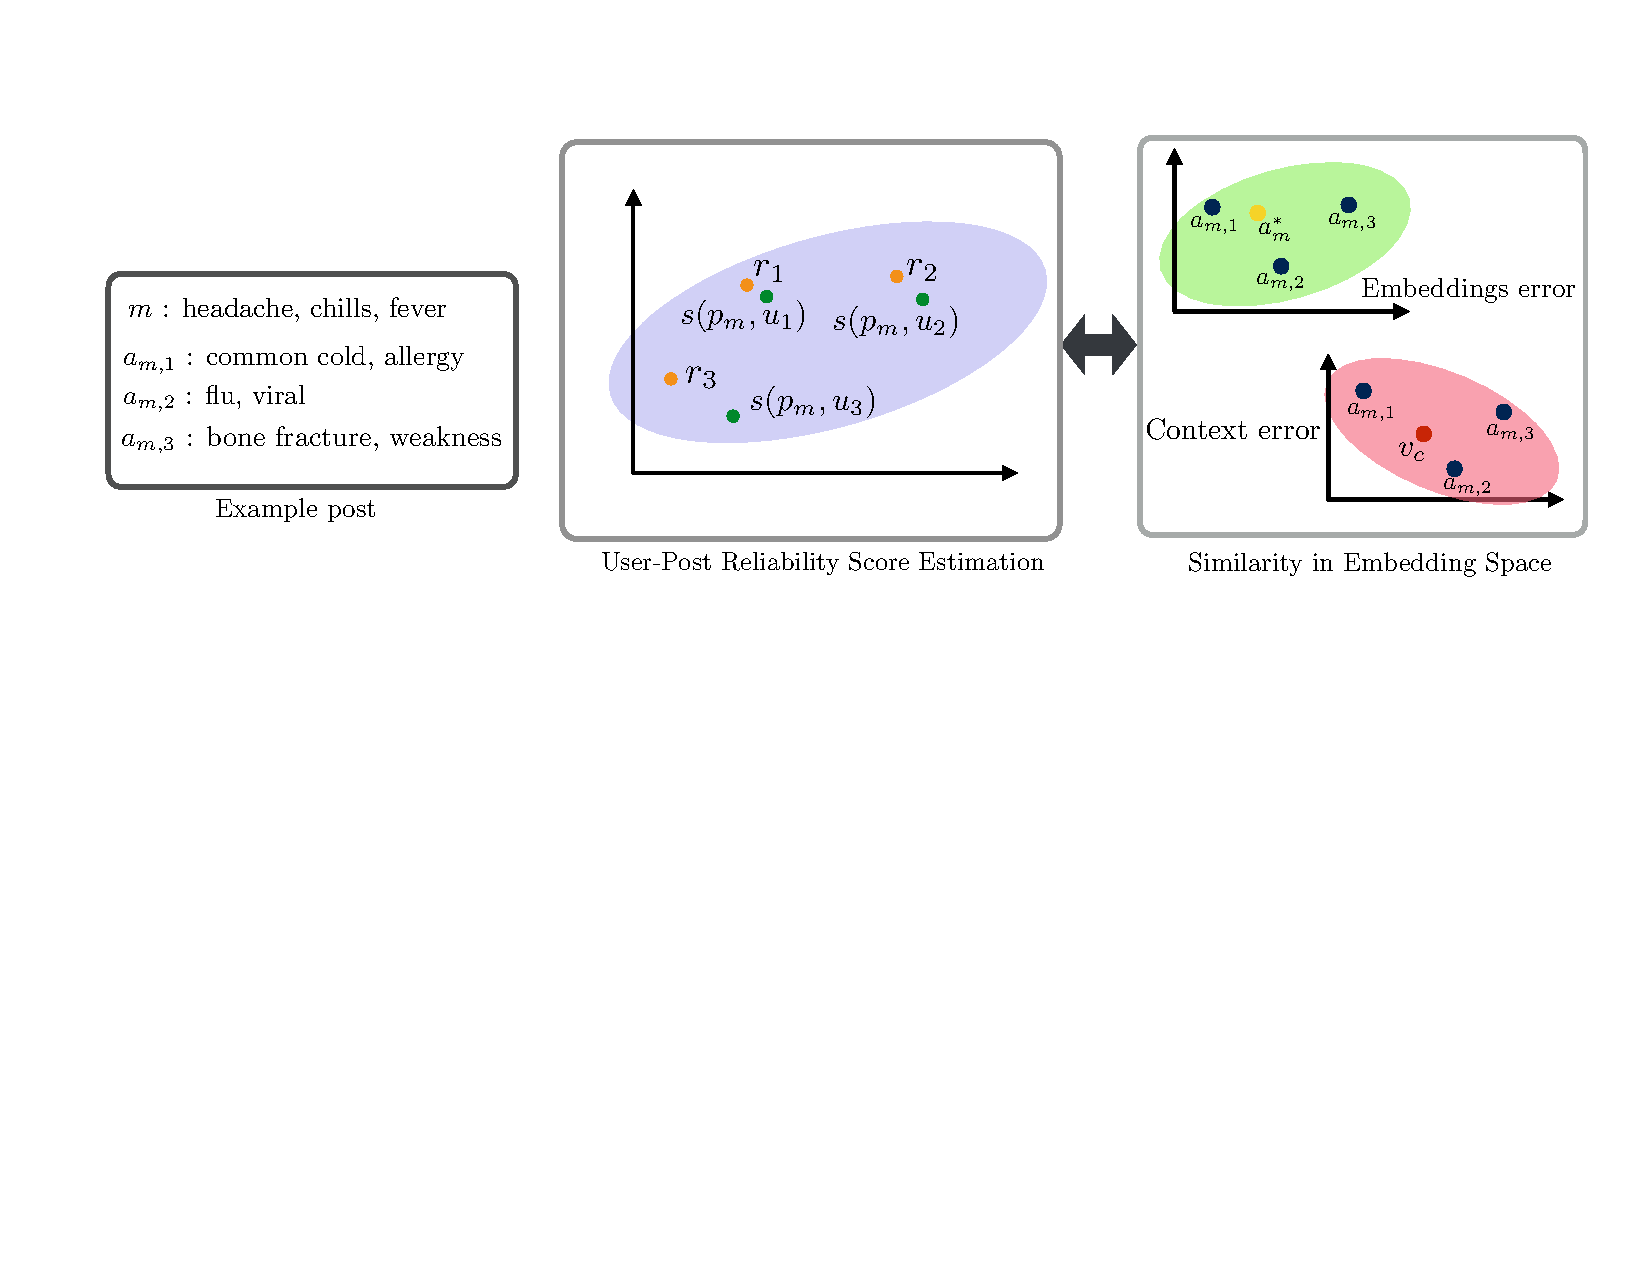
\includegraphics[scale=0.6]{images/architecture_gray_post_combined.pdf}
\caption{\small An illustrative toy example detailing our model components.
The left-hand side details the user-post reliability score estimation, $R_{m,n}$, that is a function of similarity function $s(.)$ between the user and post aspect distributions and user aspect reliabilities, $\bm{r}_n$. In the right-hand, we learn trustworthy comment embedding, $\bm{a}_m^{*}$, such that it is similar to user comments, $\bm{a}_{m,n}$ which are, in turn, similar to the post context $\bm{v}_c$.
}
\label{fig:model}
\end{figure}

\subsection{Solving the Optimization Problem}
We use coordinate descent \cite{bertsekas1999nonlinear} to solve our optimization problem. In particular, we solve the equation for each variable while keeping the rest fixed.

\paragraph{Case 1:}
Fixing $\{\bm{r}_n\}$ and $\{ \bm{v}_{\omega} \}$
, we have the following update equation for $ \{ \bm{a}_m^* \}$:
 {\small
\begin{align}
\bm{a}_m^* = \frac{ \sum_{n \in \mathcal{N}_m} R_{m,n} \bm{a}_{m,n} } { \sum_{n \in \mathcal{N}_m} R_{m,n} }
\end{align}
}
Thus, the latent \emph{trustworthy comment} is a weighted combination of comments where weights are provided by the \emph{user-post reliability} score $R_{m,n}$.
Alternatively, it can also be interpreted as a reliable summarization of all the comments.
\paragraph{Case 2:}
Fixing $\{ \bm{a}_m^* \}$, $\{ \bm{v}_{\omega} \}$
, we have the following update equation for $ \{\bm{r}_n^{(k)}\}$:
\begin{equation}
\resizebox{0.55\linewidth}{!}{$
\begin{aligned}
\bm{r}_n^{(k)} \propto - \ln {\sum_{m \in \mathcal{M}_n} s(\bm{u}_{n}^{(k)} , \bm{p}_{m}^{(k)}) \left( E_{m,n} + {\beta } Q_{m,n} \right)}
\end{aligned}
$}
\end{equation}
Reliability of a user in aspect $k$ is inversely proportional to the errors with respect to the latent trustworthy comment $\bm{a}_m^{*}$ ($E_{m,n}$) and submission's context $\bm{v}_c$ ($Q_{m,n}$) over all of her posted comments ($\mathcal{M}_n$). The embedding error ensures that if there is a large difference between the user's comment and the trustworthy comment, her reliability becomes lower. The context error ensures that non-relevant comments to the post's context are penalized heavily. In other words, a reliable user should give trustworthy and contextualized responses to posts.

This error is further weighed by the similarity score, $s(.)$, capturing familiarity of the user with the post's context. Thus, familiar users are penalized higher for their mistakes as compared to unfamiliar users.

\paragraph{Case 3:}
Fixing $\{ \bm{a}_m^* \}, \{\bm{r}_n^{(k)}\}$,
we have the following update equation for $\{ \bm{v}_{\omega} \}$:
\begin{equation}
\resizebox{.85\hsize}{!}{$
\begin{aligned}
 \bm{v}_{\omega} &= \frac{\sum_{<m,n> \in D_{\omega}} R_{m,n}\left( \bm{a}_m^* + \beta \vert c_m \vert^{-1} \sum_{c \in c_m} \bm{v}_c \right)
 - R_{m,n} (\beta + 1)\vert c_m \vert^{-1} \bm{a}_{m,n}^{- \omega} }{ \sum_{<m,n> \in D_{\omega}} R_{m,n}(\beta + 1)}
\end{aligned}
$}
\end{equation}
where $<m,n> \in D_{\omega} = \{ (m,n) \vert \omega \in w_{m,n} \}$ and $\bm{a}_{m,n}^{-\omega} = \vert w_{m, n} \vert^{-1} \sum_{\omega' \in w_{m,n} \setminus \{ \omega \} } \bm{v}_{\omega'}$. To update $\bm{v}_\omega$, we only consider those comment and submission pairs, $D_{\omega}$, in which the particular word appears.
The update of the embeddings depend on the submission context $\bm{v}_c$, latent trustworthy comment embedding, $\bm{a}_m^*$ as well as \emph{user-post reliability} score, $R_{m,n}$. Thus, word embeddings are updated in a trust-aware manner such that reliable user's comments weigh more than those of unreliable users as they can contain noisy text. Note that there is also some negative dependency on the contribution of other terms in the comments.

\noindent
\textbf{Implementation Details:}
We used popular Latent Dirichlet Allocation (LDA)~\cite{blei2003latent} to estimate aspects of the posts in our dataset\footnote{We ran LDA with 50 topics for all experiments and examined its sensitivity in Section \ref{Results}.}. Specifically, we combined the title and body text to represent each post. We applied topic model inference to all comments of user $n$ to compute its combined aspect distribution, $\bm{u}_n$.
We randomly initialized the user reliability, $\bm{r}_n$. We initialized the word embeddings, $\bm{v}_\omega$, via word2vec~\cite{mikolov2013distributed} trained on our dataset. We used both unigrams and bigrams in our model. We fixed $\beta$ to $0.15$.\footnote{We did not find a significant change in results for different values of $\beta$.}
The model converges after only about six iterations indicating quick approximation.
In general, the computational complexity is $O(\vert \mathcal{V} \vert N M)$; however,
we leverage the data sparsity in the comment-word usage and user-posts for efficient implementation.

\section{Experiments} \label{subsec:experiments}
In this section, we first discuss our novel dataset, followed by experiments on the outputs learned by our model. In particular, we evaluate the trustworthy comment embeddings on the comment ranking task while we qualitatively evaluate user reliabilities and word embeddings. For brevity, we focus the qualitative analysis on our largest subreddit, askscience.
\subsection{Dataset} \label{subsec:dataset}
We evaluate our model on a widely popular discussion forum Reddit. Reddit covers diverse topics of discussion and is challenging due to the prevalence of noisy responses.

\begin{table}[tbh]
  \centering
\begin{tabular}{  p{20mm}| r | r | r | r | r | r}
\toprule
  Dataset & Created & $N$ & \textbf{$N_e$} & \textbf{$M$} & \textbf{$\vert a_{m,e} \vert$} & \textbf{$\vert w_{m,n} \vert $} \\ %\hline
  \midrule
 *Docs & 07/13 & 3,334 & 286 & 17,342 & 10,389 & 53.5 \\
 *Science & 04/10 & 73,463 & 2,195 & 100,237 & 70,108 & 74.0\\
*Historians & 08/11 & 27,264 & 296 & 45,650 & 30,268 & 103.4 \\
 \bottomrule
\end{tabular}
\caption{\label{tab:redditdata} Dataset statistics for the subreddit communities. The symbol meaning are as follows: $N$ and $M$ denotes total users and posts respectively; $N_e$: number of experts; $\vert a_{m, e} \vert$: number of posts with at least one expert comment; $\vert w_{m, n} \vert$: average comment word length. }
\end{table}

We specifically tested on \emph{Ask*} subreddits as they are primarily used to seek answers to a variety of topics from mundane issues to serious medical concerns. In particular, we crawled data from three subreddits, /r/askscience, /r/AskHistorians, and /r/AskDocs from their inception until October 2017 \footnote{\url{praw.readthedocs.io/en/latest/} }. While these subreddits share the same platform, the communities differ vastly, see Table \ref{tab:redditdata}. We preprocessed the data by removing uninformative comments and posts with either less than ten characters or containing only URLs or with a missing title or author information.
We removed users who have posted less than two comments and also submissions with three or fewer comments. To handle sparsity, we treated all users with a single comment as "UNK".


\begin{figure}[tbh]
\centering
  \begin{subfigure}{0.5\textwidth}
  \centering
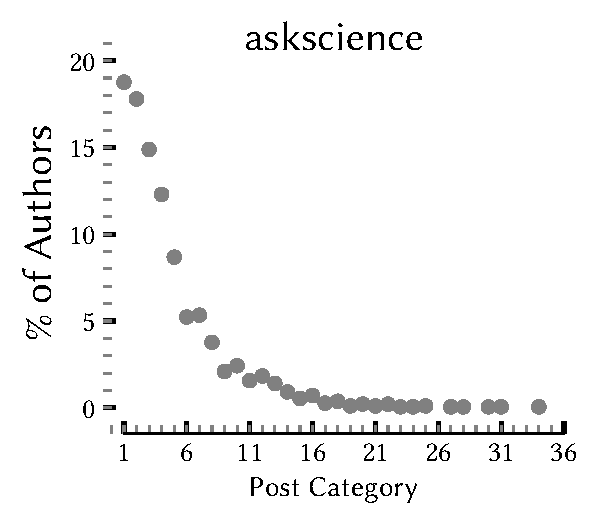
\includegraphics[scale=0.62]{images/Flair_frequency.pdf}
\end{subfigure}%
  \begin{subfigure}{0.5\textwidth}
  \centering
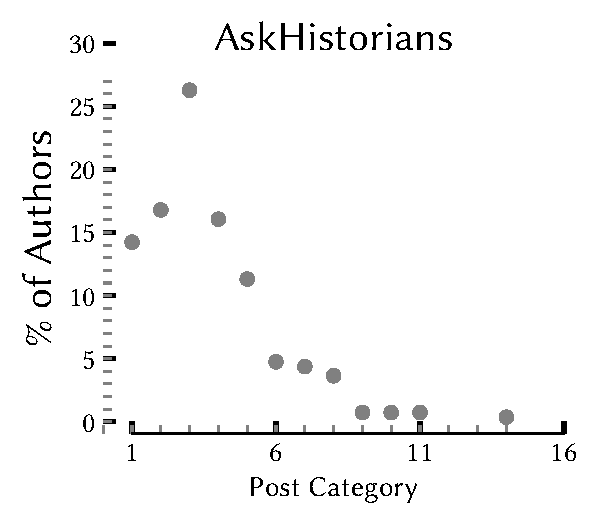
\includegraphics[scale=0.62]{images/Flair_frequency_askhistory.pdf}
\end{subfigure}
\caption{Frequency plot of \% of authors commenting on the post with unique submission flairs.}
\label{fig:flair}
\end{figure}

\begin{figure}
  \centering
  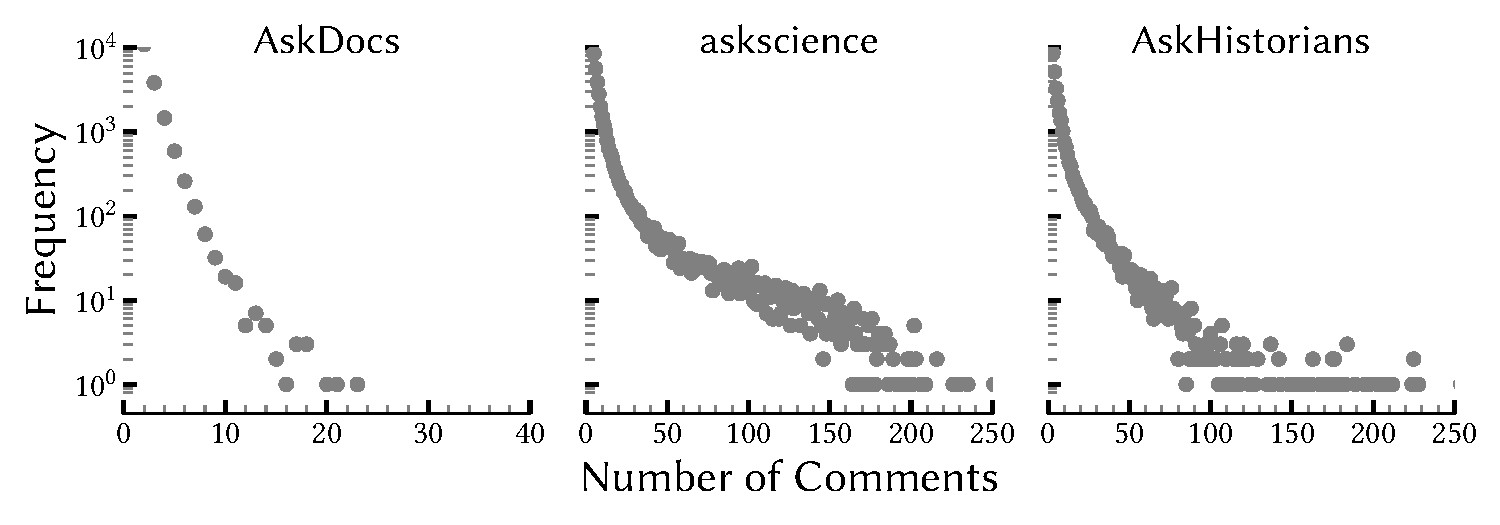
\includegraphics[scale=0.62]{images/Frequency}
  \caption{Frequency plot (log scale) of number of comments per post for three subreddits. A post on AskDocs tend to have fewer comments than the other two communities.}
  \label{fig:frequency}
\end{figure}

For each submission post,
there is a flair text denoting the subtopic of the post, referred as the \textit{submission flair} that is either Moderator added or self-annotated. We denote \emph{submission flair} as the \emph{category} of the post, e.g. Physics, Chemistry, Biology are some categories in AskScience. Similarly, users have \textit{author flairs} attributed next to their user-name, e.g. Astrophysist, Bioengineering. They describe the user's educational background and help the OP in assessing user reliability. In order to get verified and obtain a flair, the users must send the moderators anonymized verification documents, including certification numbers, contact information. We denote verified users with \textit{author flairs} as experts in the rest of the paper.
Table \ref{tab:redditFlairText} presents frequent submission and author flairs for all the subreddits.
AskDocs does not have submission flairs as it is a smaller community.
Figure \ref{fig:flair} shows the distribution of the authors with the number of unique categories of the posts where the user commented. For both subreddits, we observed that around 80\% of the users comment on posts from more than two categories. This shows that users engage with a variety of topics in Reddit.


\begin{table*}[t]
  \centering
\begin{tabular}{ l | p{6cm} | p{6cm}}
\toprule
  Sub-Reddit & Author Flairs & Submission Flairs\\
  \midrule
 *Docs & Physician, Medical Student, Registered Nurse, Physician Assistant, Pharmacist, Nursing Student, Pharmacy Student, EMT, Doctor, Moderator, M.D., Nurse Practitioner     & NA  \\
\hline
 *Science & Biochemistry, Molecular Biology, Immunology, Genetics, Microbiology, Neuroscience, Bioinformatics, Astrophysics, Biophysics, Cell Biology, Materials Science, Cosmology & Physics, Biology, Astronomy, Chemistry, Engineering, Medicine, Earth Sciences, Mathematics, Neuroscience, Computing, Human Body, Planetary Sci. \\
\hline
*Historians & Early Christianity, Ancient Near East, Andean Archaeology, Interesting Inquirer, Colonialism, Mesoamerican Archaeology, New Spain, American Civil War, Holocaust, Medieval Europe, Early Modern Europe, Environment & AMA, Urbanism, Fashion, Myth, Floating, Africa, Literature, Best Of, Pop Music, Home, Death, South America, Trade \\
 \bottomrule
\end{tabular}
%}
\caption{ Top-K most frequent author and submission flairs that appear in our dataset, these flairs are used only in evaluation as our model is unsupervised.  }
\label{tab:redditFlairText}
\end{table*}

Experts are highly active in the community, they answer around 60-70\% of the posts (Table \ref{tab:redditdata}). askscience and AskHistorians have significantly higher and more detailed comments ($\vert w_{m, n} \vert$ in Table \ref{tab:redditdata}) per post than AskDocs, as shown in Figure \ref{fig:frequency}. Due to the prevalence of a large number of comments, manual curation is very expensive, thus necessitating the need for an automatic tool to infer trustworthiness of the comments.

\subsection{Experimental Setup}
We evaluate latent trustworthy comment learned by our model on a trustworthy comment ranking task. That is, given a submission post, our goal is to rank the posted comment based on their trustworthiness.
For this experiment, we treat expert users' comment as the most trustworthy comment of the post.\footnote{While human judgment would be the most precise; it is also the most challenging to collect. For instance, in askscience we would need experts in over 35 science fields, reading up to 250 comments for a single post.}
Besides, we also report results using the highest upvoted comment as the gold standard. Highest upvoted comments represent community consensus on the most trustworthy response for the post \cite{Voting:2019}. While it is shown that there is widespread under-provision on Reddit, and thus, it is possible to miss high-quality content that is not highly voted; nevertheless, upvotes is a good proxy for community consensus~\cite{gilbert2013widespread}.

In particular, we rank comments for each post $m$, in the order of descending cosine similarity between their embedding, $\bm{a}_{m,n}$, and the latent trustworthy comment embeddings, $\bm{a}_m^*$. We then report average Precison@k values over all the posts, where k denotes the position in the output ranked list of comments.


\noindent
\textbf{Baselines:} We compare our model with state-of-the-art truth discovery methods proposed for continuous and text data and non-aspect version of our model. Note that there is no label information used, so we cannot compare to other supervised CQA models \cite{Quality2008,wen2018hybrid,nakov2017semeval} which need this supervision. Our \emph{unsupervised model} is complementary to these approaches, and thus, a rigorous comparison is impossible.


\noindent
\emph{Mean Bag of Answers (MBoA)}: In this baseline, we represent the trustworthy comment for a post as the mean comment embedding. This baseline assumes uniform user reliability.

\noindent
\emph{CRH}: is a state-of-the-art truth discovery-based model for heterogeneous data, i.e. categorical and numerical data~\cite{li2014resolving}. CRH minimizes the weighted deviation of the trustworthy comment embedding from the individual comment embeddings with user reliabilities providing the weights.

\noindent
\emph{CATD}: is an extension of CRH that learns a confidence interval over user reliabilities to handle data skewness~\cite{li2014confidence}. For both the above models, we represent each comment as the average word embeddings of its constituent terms.

\noindent
\emph{TrustAnswer}: Li et al.~\cite{li2017reliable} modeled semantic similarity between comments by representing each comment with embeddings of its key phrase.

\noindent
\emph{CrowdQM-no-aspect:} In this baseline, we condense the commenter's aspect reliabilities to a single $r_n$ and simplify the \emph{user-post reliability} score computation. The updated optimization equation  is,

\begin{equation}
\begin{aligned}
\underset{\{a_m^{*}\}, \{v_{\omega}\}, \{r_n\}  }{\text{min}}
\sum_{n=1}^{N} r_n \left( \sum_{m \in \mathcal{M}_n} s(\bm{u}_{n}, \bm{p}_{m}) \left( E_{m, n} + \beta \odot Q_{m, n} \right) \right)  \\
\text{s.t.  } \sum_{n=1}^{N} e^{-r_n} = 1
\end{aligned}
\end{equation}

This model acts as a control to gauge the performance of our proposed model.

We do not compare with other truth discovery methods ~\cite{Zhao:2012, Yin:2007, Pasternack:2011, Galland:2010, Dong:2009} as CRH and CATD are already shown to outperform them.

\subsection{Results}\label{Results}
Table \ref{tab:pred} reports the Precision@1 results using expert's comments as gold standard.
MBoA, with uniform source reliability, outperforms the CRH method that estimates reliability for each user separately. Thus, simple mean embeddings provide a robust representation for the trustworthy comment.
\begin{table}[tbh]
  \centering
\begin{tabular}{ l | c c c }
\toprule %\hline
 Model &  *Docs & *Science & *Historians \\
  \midrule
 MBoA             & 0.592 & 0.633 & 0.602 \\
 CRH                                     & 0.585 & 0.597 & 0.556 \\
 CATD                                 & \textbf{0.635} & 0.700 & 0.669 \\
 TrustAnswer                     & 0.501 & 0.657 & 0.637 \\
 CrowdQM-no-aspect                           & 0.509 & 0.666 & 0.640 \\
 CrowdQM            & 0.617 & \textbf{0.734} & \textbf{0.753} \\
 \bottomrule
\end{tabular}
% }%
\caption{\label{tab:pred} Precision@1 for all three Ask* subreddits, where the experts' comments are treated as the trustworthy comment. }
\end{table}

We also observe that CrowdQM-no-aspect performs consistently better than TrustAnswer. Note that both approaches do not model aspect-level user reliability but use semantic representations of comments. However, while TrustAnswer assigns a single reliability score for each comment, CrowdQM-no-aspect additionally takes into account the user's familiarity with the post's context (\emph{similarity} function, $s(.)$)
to compute her reliability for the post.
Finally, CrowdQM consistently outperforms both the models, indicating that aspect modeling is beneficial.

CATD uses a confidence-aware approach to handle data skewness and performs the best among the baselines. This skewness is especially helpful in Reddit as experts are the most active users (Table \ref{tab:redditdata}); and, CATD likely assigns them high reliability.
Our model achieves competitive precision as CATD for AskDocs while outperforming for the others. This indicates that our data-driven model works better for communities which are less sparse (Section \ref{subsec:dataset} and Figure \ref{fig:frequency}).

\begin{figure*}[tbh]
\begin{subfigure}{\linewidth}
\centering
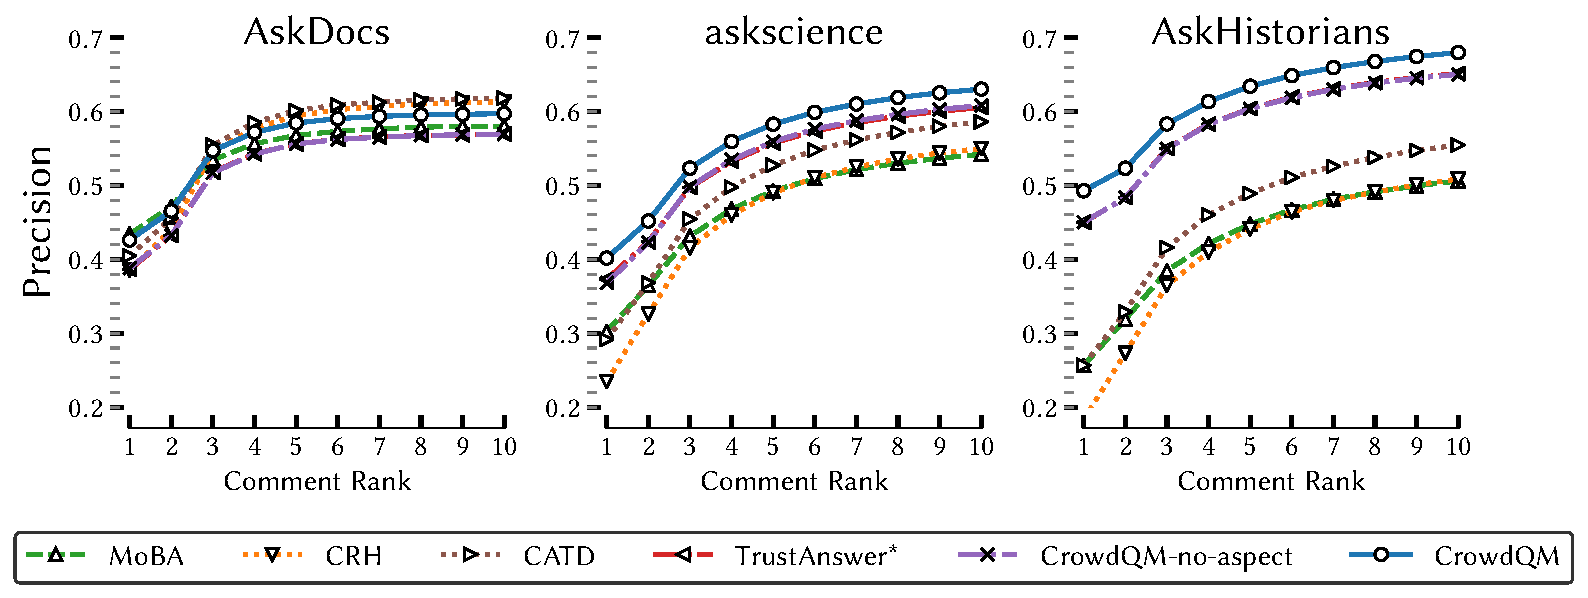
\includegraphics[scale=0.61]{images/Precision.pdf}
\end{subfigure}%
\caption{\label{fig:comment}Precision of our model vs. comment rank computed by user's upvotes. Our model outperforms the baselines for askscience and AskHistorians while performs similarly for AskDocs.}
\end{figure*}

\begin{table}[tbh]
  \centering
\begin{tabular}{l | c c c }
\toprule %\hline
 Model &  *Docs & *Science & *Historians \\
  \midrule
 MBoA                 & \textbf{0.434} & 0.302 & 0.257 \\
 CRH                                         & 0.386 & 0.234 & 0.183 \\
 CATD                                     & 0.405 & 0.291 & 0.257 \\
 TrustAnswer                         & 0.386 & 0.373 & 0.449  \\
 CrowdQM-no-aspect                               & 0.388 & 0.368 & 0.450  \\
 CrowdQM                  & 0.426 & \textbf{0.402} & \textbf{0.493}  \\
 \bottomrule
\end{tabular}
% }%
\caption{\label{tab:pup} Precision@1 for all three Ask* subreddits, where the highest upvoted comment is  treated as the most trustworthy comment.}
\end{table}

Table \ref{tab:pup} reports Precision@1 results using community upvoted comments as the gold standard, while Figure \ref{fig:comment} plots the precision values against the size of the output ranked comment list. In general, there is a drop in performance for all models on this metric because it is harder to predict upvotes as they are inherently noisy~\cite{gilbert2013widespread}.

TrustAnswer and CrowdQM-no-aspect perform best among the baselines indicating that modeling semantic representation is essential for forums. CrowdQM again consistently outperforms the non-aspect based models verifying that aspect modeling is needed to identify trustworthy comments in forums.

CrowdQM remains competitive in the smaller AskDocs dataset, where the best performing model is MoBA. Thus, for AskDocs, the comment summarizing all other comments tends to get the highest votes.

\begin{figure*}[tbh]
\begin{subfigure}{\linewidth}
\centering
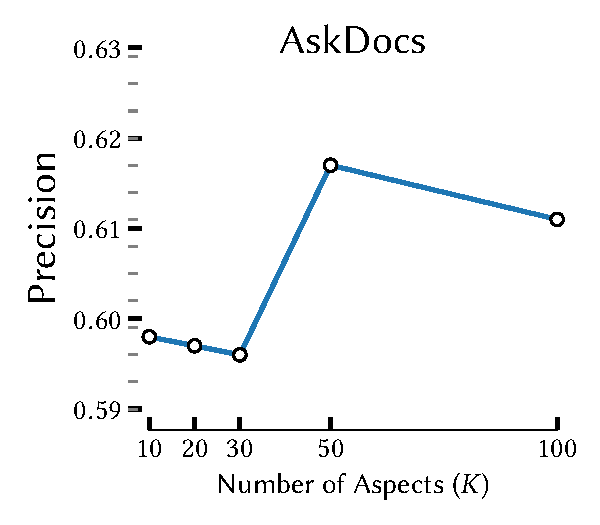
\includegraphics[scale=0.67]{images/Precision_aspect.pdf}
\end{subfigure}
\caption{\label{fig:aspect} Precision of our model with changing number of aspects. Value of $K$ does not have much impact on the precision value.}
\end{figure*}

\textbf{Parameter Sensitivity} In Figure \ref{fig:aspect}, we plot our model's precision with varying number of aspects. Although there is an optimal range around 50 aspects, the precision remains relatively stable
indicating that our model is not sensitive to number of aspects. We also observed similar results for the other datasets and omitted those figures for lack of space. We also did similar analysis with $\beta$ and did not find any significant changes to the Precision.


\subsection{Model Convergence}
\begin{figure}[!h]
\begin{subfigure}{.5\linewidth}
  \centering
  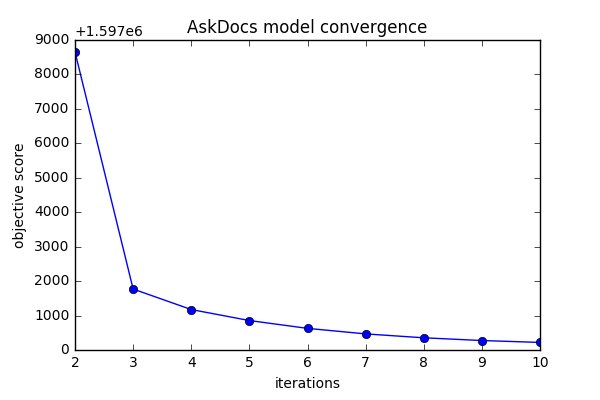
\includegraphics[width=0.9\linewidth]{images/AskDocs_model_convergence.png}
  \caption{AskDocs}
  \label{fig:AskDocsfig1}
\end{subfigure}%
\begin{subfigure}{.5\linewidth}
  \centering
  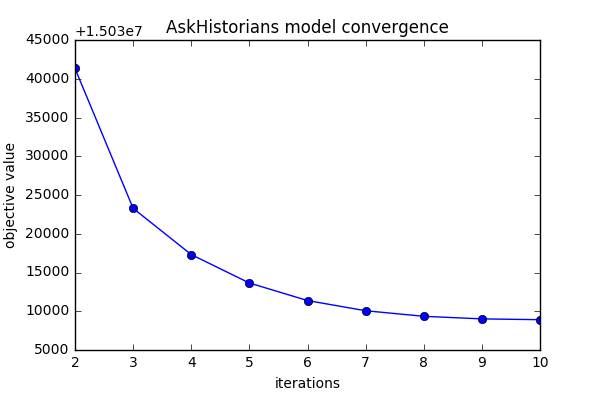
\includegraphics[width=0.9\linewidth]{images/AskHistorians_model_convergence.png}
  \caption{AskHistorians}
  \label{fig:AskHistoriansfig1}
\end{subfigure}
\hspace{6em}
\begin{subfigure}{\textwidth}
  \centering
%   \begin{center}
  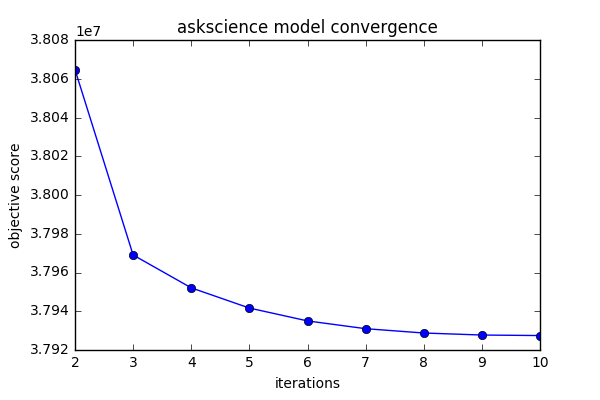
\includegraphics[width=0.49\linewidth]{images/askscience_model_convergence.png}
%   \end{center}
  \caption{askscience}
  \label{fig:asksciencefig1}
\end{subfigure}
\caption{CrowdQM model convergence for AskDocs, AskHistorians, and askscience respectively.}
\label{fig:convergence}
\end{figure}
In Figure \ref{fig:convergence}, we plot the objective function score at each iteration, for our model CrowdQM for the three subreddits. On all three subreddits, the model converges after only about six iterations indicating our model is quick to approximate a solution. In general, the computational complexity is $O(\vert \mathcal{V} \vert N M)$ for a single iteration. However, our implementation leverages the data sparsity in the comment-word usage and user-submissions posts to make the model efficient.

\section{Discussion} \label{sec:discussion}
In this section, we report qualitative analysis of user-aspect reliabilities \{$r_n$\} and word embeddings \{$v_w$\} learned by our proposed CrowdQM model. For brevity, we focus our analysis on our largest subreddit, askscience.

\subsection{Aspect Reliability Analysis}
We evaluate learned user reliabilities through users commenting on a post with a \emph{submission flair}. A submission flair is manually curated and denotes post's category, and this information is not used in our model. Specifically, for each post $m$, we compute the \emph{user-post reliability} score, $R_{m,n}$, for every user $n$ who commented on the post. We then ranked these scores for each category and report top-10 \emph{author flairs} for few categories in Table \ref{tab:modelAlignment2}.

\begin{spacing}{1}
\begin{longtable}{l}
\caption[Author flairs per post categories]{Most reliable author flairs with their corresponding post categories according to user-post reliability score, $R_{m, n}$.
} \\
\hline  \toprule
\endfirsthead

\hline
{\bfseries \tablename\ \thetable{} -- continued from previous page} \\ \hline
\endhead

\hline %{\bfseries \tablename\ \thetable{} Continued on next page} \\\hline
\endfoot

%\hline
\endlastfoot
 \multicolumn{1}{c}{Post Category: Computing} \\ \hline
Embedded Systems, Software Engineering , Robotics \\
Computer Science \\
Quantum Optics, Singular Optics \\
Robotics, Machine Learning, Computer Vision, Manipulators \\
Computer Science \\
High Performance Computing, Network Modeling and Simulation \\
Biomechanical Engineering, Biomaterials \\
Machine Learning, Deep Architectures, Scientific Computing  \\
Machine Learning, Deep Architectures, Scientific Computing\\
Programming Languages, Computer Security \\
\hline

\multicolumn{1}{c}{Post Category: Archaeology} \\ \hline
Archaeology, Maya Stone Tools, Geoscience \\
Global Health, Tropical Medicine \\
Control, Robotics Engineering, Industrial Robotics \\
Archaeology, Collapse of Complex Societies \\
Archaeology, Archaeometallurgy \\
Criminal Justice  \\
Computational and Evolutionary Archaeology \\
Evolutionary Biology, Plant-Herbivore Systems \\
Computational and Evolutionary Archaeology \\
Archaeology, Collapse of Complex Societies \\
\hline

\multicolumn{1}{c}{Post Category: Biology} \\ \hline
Animal Cognition  \\
Cell and Developmental Biology  \\
Biochemistry, Molecular Biology, Enzymology  \\
Genetics, Cell biology, Bioengineering \\
Computational Physics, Biological Physics \\
Aquatic Ecology and Evolution, Active Acoustics \\
Genomic Instability, Cancer Development \\
Biochemistry, Genomics, Proteomics, Mass Spectrometry \\
Neuroscience, Psychopharmacology \\
Genetics and Genomic Sciences \\
\hline
\multicolumn{1}{c}{{Post Category:Linguistics}} \\ \hline
Linguistics, Hispanic Sociolinguistics  \\
Comparative Political Behaviour \\
Historical Linguistics, Language Documentation \\
Linguistics, Hispanic Sociolinguistics \\
Historical Linguistics, Language Documentation  \\
Cognitive Modeling \\
Nanostructured Materials, Heterogeneous Catalysis \\
Auditory Science  \\
Cognitive Modeling \\
Linguistics, Phonetics and Phonology, Sound Change \\
\hline

\multicolumn{1}{c}{{Post Category: Medicine}} \\ \hline
Infectious Diseases, Pulmonary Immunology \\
Biomedical Engineeering, Biomechanics, Biomaterials \\
Pediatric Neurology \\
Anesthesiology, Post-Operative Pain, Traumatic Brain Injuries \\
Molecular Biology, Musculoskeletal Research \\
Immunology, Immune Regulation, Infectious Diseases  \\
Molecular Biochemistry, DNA Damage Repair \\
Virology, Molecular Biology, Orthopoxviruses \\
Veterinary Medicine, Canine Lymphoma \\
Bioengineering, Cardiovascular Imaging  \\
\hline

\multicolumn{1}{c}{{Post Category: Psychology}} \\ \hline
Clinical Psychology, Psychotherapy, Behavior Analysis  \\
International Relations, Comparative Politics  \\
Neuropsychology \\
Psychology, PTSD, Trauma, and Resilience  \\
Cognitive Neuroscience, Neuroimaging, fMRI  \\
Psychology, Legal psychology, Eyewitness testimonies   \\
Experimental Psychology, Social Cognition and Statistics  \\
Clinical Psychology   \\
Clinical Psychology, Sleep, Insomnia \\
Visual Cognition, Cognitive Neuroscience  \\
\bottomrule
%\end{tabular}
\label{tab:modelAlignment2}
\end{longtable}
\end{spacing}

The top-performing \emph{author flairs} for each category are experts for that domain.
For instance, for the Computing category highly reliable users have author flairs like Software Engineering and Machine Learning, while for Linguistics authors with flairs Hispanic Sociolinguistics and Language Documentation rank high. These results align with our hypothesis that in-domain experts should have higher reliabilities.
We also observe that few out of domain authors being ranked high, such as, authors with flairs like Comparative Political Behavior and Nanostructured Materials in the Linguistic category. This diversity could be due to the interdisciplinary nature of that domain.
Our model, thus, can be used by the moderators of the discussion forum to identify and recommend potential reliable users to respond to new submission posts of a particular category.

\begin{figure}[h]
%\vspace{-0.1in}
  \begin{subfigure}{0.5\textwidth}
  \centering
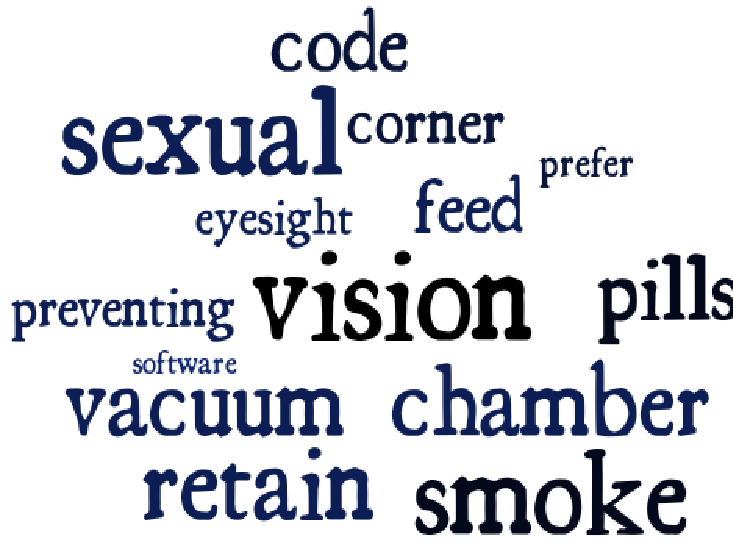
\includegraphics[scale=0.5]{images/Health.pdf}
\caption{Health}
\end{subfigure}
  \begin{subfigure}{0.5\textwidth}
  \centering
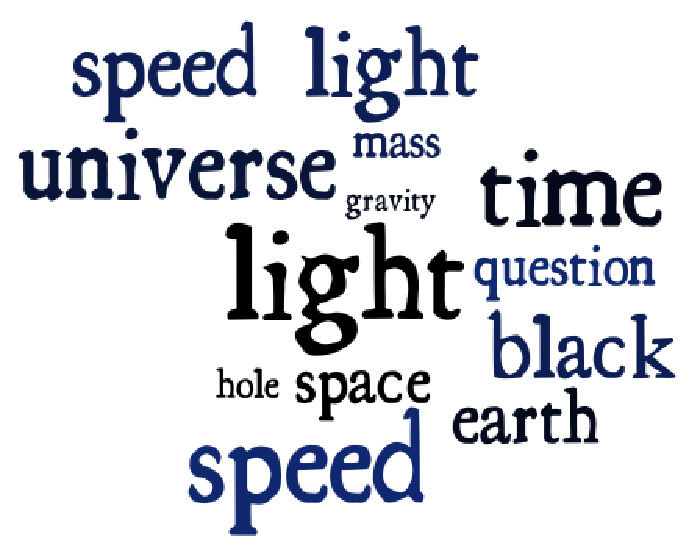
\includegraphics[scale=0.5]{images/Cosmos.pdf}
\caption{Cosmos}
\end{subfigure}
  \begin{subfigure}{0.5\textwidth}
  \centering
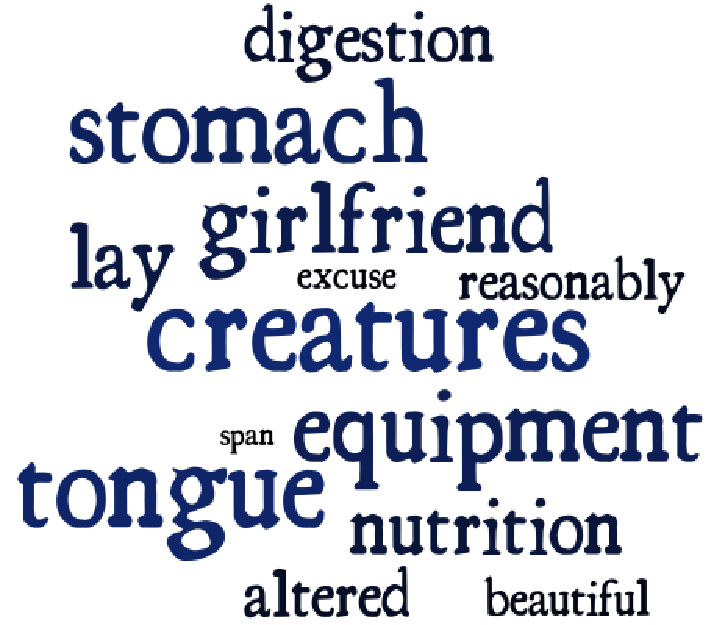
\includegraphics[scale=0.5]{images/Diabetes.pdf}
\caption{Diabetes}
\end{subfigure}
  \begin{subfigure}{0.5\textwidth}
  \centering
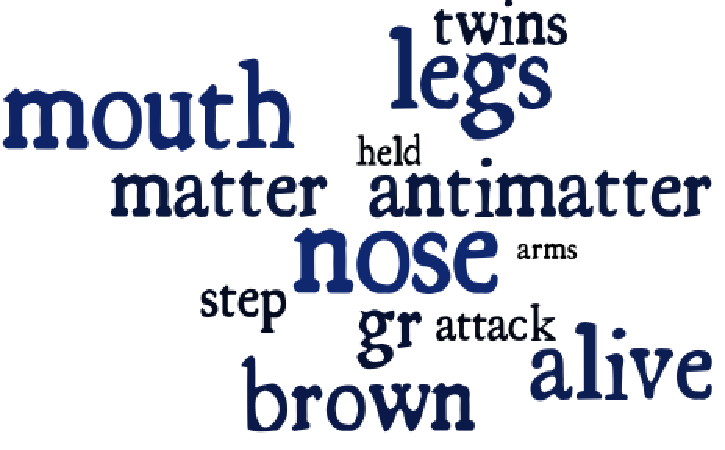
\includegraphics[scale=0.56]{images/Oceanography.pdf}
\caption{Oceanography}
\end{subfigure}
\caption{Top words for highly correlated aspects between user reliability and user karma.}
\label{fig:modelTopics}
\end{figure}

To further analyze the user reliability, we qualitatively examine the aspects with the largest reliability value of highly upvoted users in a post category. First, we identify users deemed reliable by the community for a category through a \emph{karma} score. Category-specific user \textit{karma} is given by the average upvotes the user's comments have received in the category.  We then correlate the category-specific user \textit{karma} with her reliability score in each $k \in K$ aspect, $\bm{r}_n^{(k)}$ to identify aspects relevant for that category.
Figure \ref{fig:modelTopics} shows the top words of the highest correlated aspects for some categories. The identified words are topically relevant thus our model associates aspect level user reliability coherently.
Interestingly, the aspects themselves tend to encompass several themes, for example, in the Health category, the themes are software and health. Or in the Oceanography category, the themes are around animal's physiology and matter.

\subsection{Word Embedding Analysis}

\begin{table}[tbh]
 %\captionsetup{font=small}
 \centering
 %\small
\resizebox{0.97\linewidth}{!}{
\begin{tabular}{ c | c | c | c | c | c }
\toprule
\multicolumn{2}{c| }{{Liquid}} &  \multicolumn{2}{c|}{{Cancer}} & \multicolumn{2}{c}{{Quantum}} \\ \hline
word2vec         & CrowdQM   & word2vec   & CrowdQM  & word2vec             & CrowdQM      \\ \hline
unimaginably     & gas       & mg         & disease  & search results       & model        \\
bigger so        & chemical  & curie      & white    & sis                  & energy       \\
two lenses       & solid     & wobbly     & cell     & shallower water      & particle     \\
orbiting around  & air       & subject    & food     & starts rolling       & mechanics  \\
fire itself      & material  & "yes" then & complete & antimatter galaxies  & mathematical \\
\bottomrule
\end{tabular}}\vspace{8mm}
\resizebox{0.6\linewidth}{!}{
\begin{tabular}{ c | c | c | c }
\toprule
\multicolumn{2}{c|}{{Life}} & \multicolumn{2}{c}{{Planet}} \\ \hline
word2vec      & CrowdQM    & word2vec       & CrowdQM \\ \hline
molaison      & species    & esther         & earth \\
around        & natural    & missing leg    & star \\
machos        & nature     & chimps         & plane \\
brain         & production & while drinking & land\\
"dark" matter & size       & living off     & building \\
\bottomrule
\end{tabular}
}
\caption{Similar words identified using embeddings learned by CrowdQM, and initial word2vec, for the askscience subreddit. The left and right columns correspond to word2vec and CrowdQM models respectively.}
\label{tab:WordSym}
\end{table}


The CrowdQM model updates word embeddings to better model semantic meaning of the comments. To evaluate the embeddings, we first identify the most representative aspect for each category. We denote the highest weighted aspect from the mean aspect distribution \{$\bm{p}_m$\} of all posts belonging to a category as the most representative aspect of that category.
Then, we extract frequent terms of that aspect and find its most similar keywords using cosine distance between the learned word embeddings.

The left column for each term in Table \ref{tab:WordSym} are the most similar terms returned by the initial embeddings from word2vec model while the right column reports the results from updated embeddings \{$\bm{v}_\omega$\} from our CrowdQM model.
We observe that there is a lot of noise in words returned by word2vec model as they are just co-occurrence based while words returned by our model are semantically similar and describe similar concepts. This improvement is because our model updates word embeddings in a trust aware manner such that they are similar to terms used by responses from reliable users.

\section{Conclusion} \label{sec:conclusion}
We proposed an unsupervised model to learn a trustworthy comment embedding from all the given comments for each post in a discussion forum. The learned embedding can be further used to rank the comments for that post. We explored Reddit, a novel community discussion forum dataset for this task. Reddit is particularly challenging as posts typically receive a large number of responses from a diverse set of users and each user engages in a wide range of topics.
Our model estimates aspect-level user reliability and semantic representation of each comment simultaneously in a unified optimization framework. Experiments show that modeling aspect-level user reliability improves the prediction performance compared to the non-aspect version of our model. We also show that the estimated user-post reliability can be further used to identify trustworthy users for particular post categories.

Future work includes exploring other validation methods for trustworthiness including manual annotations of the comments. Another direction is to experiment with more sophisticated methods to generate comments' semantic composition, such as recurrent neural networks. Adding learned users and comments representations to a supervised learning framework for improving them further is another interesting future research direction.


\chapter{Modeling user-to-user influence on user behavior}
%\chapter{Modeling social influence on user behavior}
\label{chap:social}
In this chapter, we model the influence of the user's explicit social connections and implicit similarity connections on their behavior. Recommender systems are a perfect example of an online platform where user preferences exhibit strong user homophily with their friends. In this work, we exploit homophily in the user and item space. Besides, user's history itself influences their preferences.
We propose separate modules to capture these different factors and later fuse them to predict future items accurately for platform users. Our model outperforms previous approaches modeling a subset of these factors \cite{social}.

\section{Overview}

Recommender systems are ubiquitous and model user preferences on commercial and social websites as well as in apps. These systems predict with reasonable accuracy, products that we may be interested in, people which we may know, or songs and movies that we may appreciate. This success builds upon a long history of research. However, to this day, a large active community continues to improve recommender systems as many questions remain open, e.g., How to effectively model and merge multiple factors influencing user preferences like (1) temporal context, (2) social influence, and (3) similarity between items? We explore this question in detail in this chapter.

Classic collaborative filtering is one of the most successful approaches to model user preferences. It learns a low dimensional and often linear latent factor model for both users and items via matrix factorization of the user-item interaction matrix~\cite{Rendle}. With deep learning taking a more prominent role, more complex models have been applied to learn increasingly non-linear relationships~\cite{NeuMF, CDAE}.
However, those classical methods ignore all three of the factors above.
Hence, many techniques have been developed, which augment classical recommender systems with one of those factors.

First, considering temporal context removes the assumption of a static interaction matrix, which generally doesn't hold as user preferences evolve with time. Thus, history from a distant past is not necessarily relevant to current preferences.
To this end, Markov chains~\cite{Rendle2} and recently, Convolution Neural Network (CNN)~\cite{SAS:2018} and Recurrent Neural Network (RNN)~\cite{GRU4Rec} based methods have been proposed to model this temporal dependence in recommender systems.
Those methods remove the static interaction matrix of classical collaborative filtering and learn a user's and an item's hidden representation based on their recent interactions.

Second, considering social influence removes the restriction that users operate in isolation. This idea is popularized by the social influence theory~\cite{Tang:2009}, which argues that a user's preference is influenced by their friends' behavior, leading to user homophily (similar user preferences). It is noteworthy that these influences are inherently dynamic as friends' preferences are evolving too (socio-temporal influence), a fact mostly ignored by current systems.
For instance, recent works model static social effect~\cite{SBPR, Collaborative, SERec, fan2019}. These methods look at the entire history of the user's friends instead of emphasizing the most recent actions. Moreover, these approaches assume uniform importance of all friends. While this is not suitable in general, it is an important first step to understand social influence for  recommendation.

Third, exploiting similarities between items (based on co-occurrence or similar features)  alleviates the data sparsity issue %for long-tail items
(many items with few ratings). Similar items hold similar attractiveness to users, leading to item homophily. Deep net based recommender models are prone to skew prediction results towards popular items with ample feedback in the training data (overfit to popular items)~\cite{ Longtail:2018}. This is counterproductive to user experience as it leads to similar recommendations across users. Also, compared to highly frequented items, long-tail items (items with fewer ratings) result in higher profit margins for the platforms~\cite{Yin:2012}. Item-Item collaborative filtering based methods~\cite{itemCF} integrate these similarities but ignore the user's history; thus providing generic recommendations.

\begin{figure}[tbh]
  \centering
  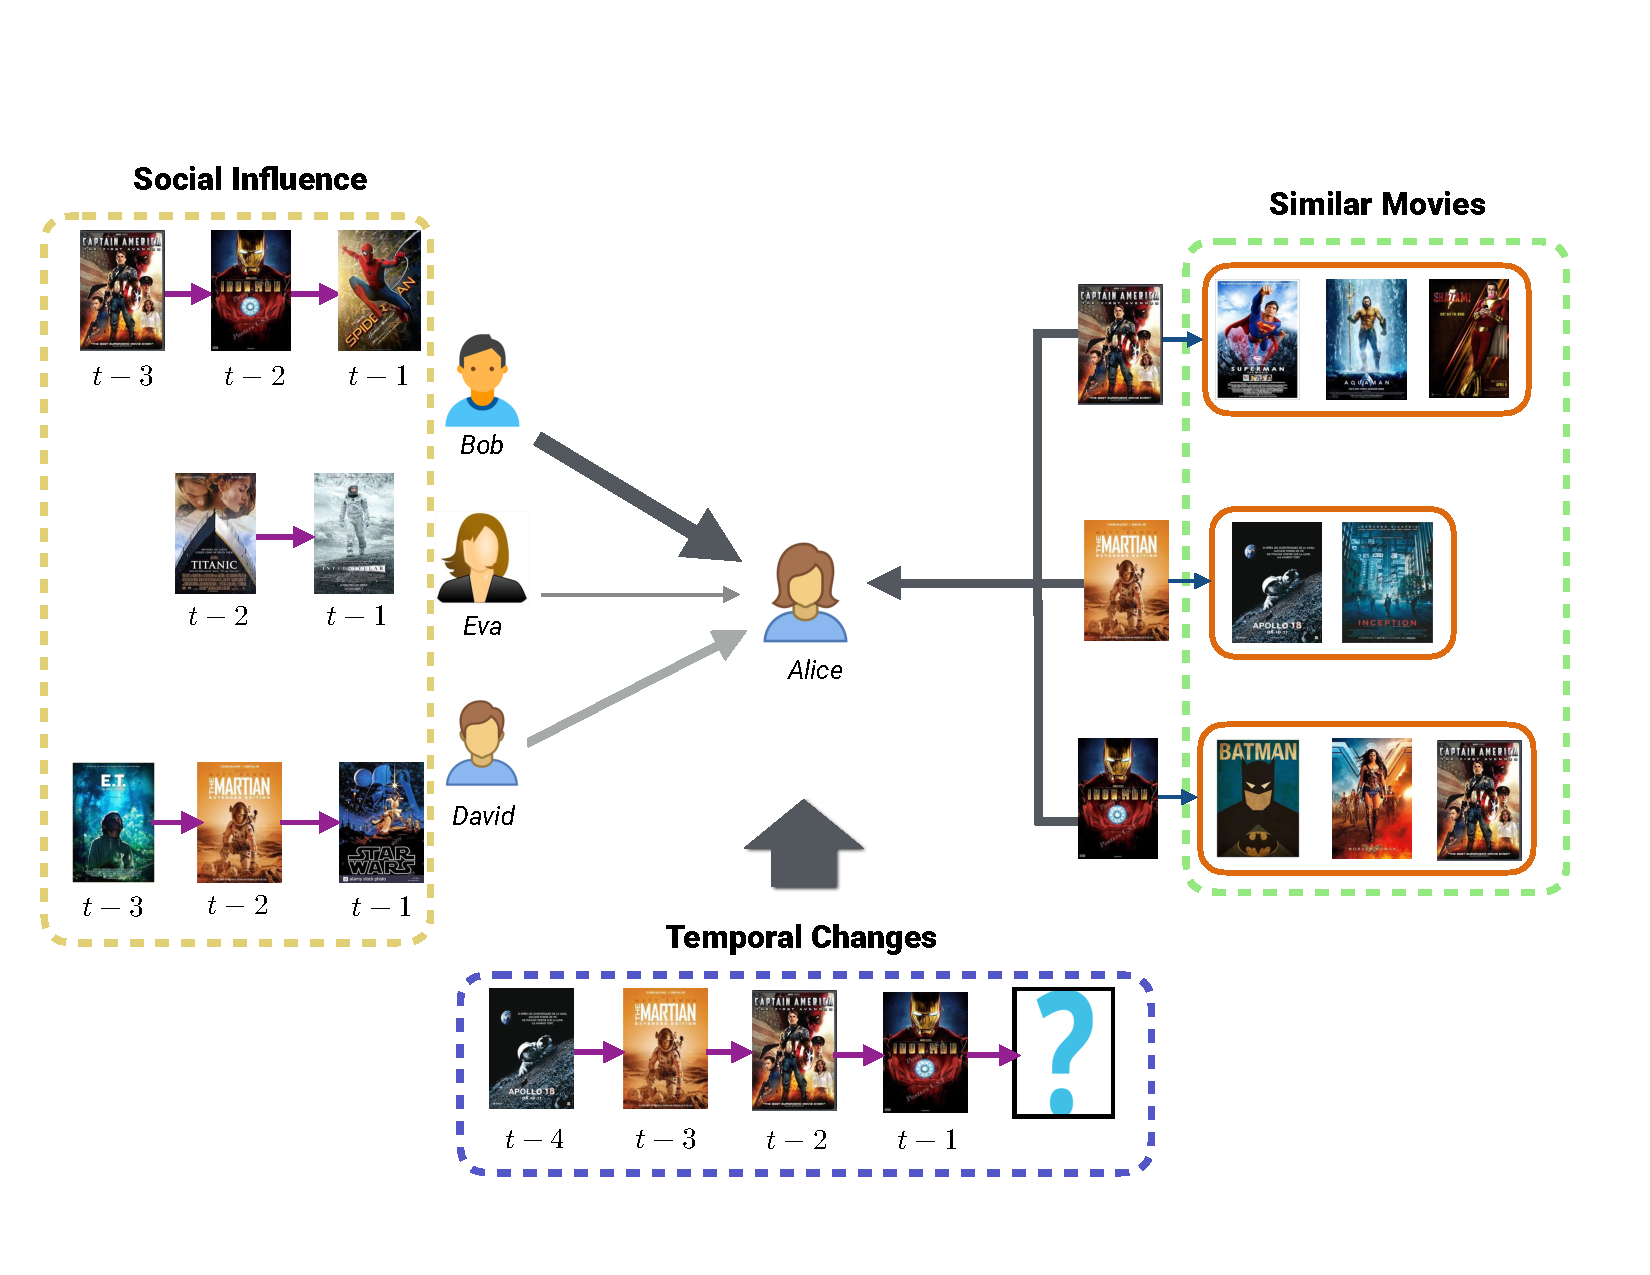
\includegraphics[width=\linewidth]{figures/Idea}
  \caption{Illustrative diagram of factors affecting Alice's decision on which movie to watch next in an online social movie viewing platform. Her current interests are towards superhero movies (temporal); she could either decide to watch recent superhero movies seen by her friends (social) or other superhero movies not watched by her friends (similar items).}
  \label{fig:Idea}
\end{figure}

To make these three points concrete, let us consider the example shown in Figure~\ref{fig:Idea}. Alice is using an online social movie viewing platform. She is currently hooked onto superhero movies (temporal). While deciding which movie to watch next, she will be influenced by recent superhero movies watched by her friends on the platform (socio-temporal influence). She could also decide to watch other superhero movies in the platform not seen by her social circle yet (item-to-item similarity).

As illustrated earlier, a user's behavior is affected by at least
the aforementioned three factors (others could include time-of-day, mood, etc.). However, the relative importance of these factors still remains unclear. It is indeed challenging to model these factors effectively and efficiently in a unified model as these cues mutually influence each other.
This is emphasized by the fact that existing work often studies only a subset of those three cues.

To address this concern, we develop a `Fusion Recommender' (FuseRec) model to jointly and efficiently capture all the factors in a unified model. It takes into account a user's temporal changes along with homophily in the user and item space. It treats each of the signals equally and combines them in an interpretable manner.

More specifically, we use three different modules to model each factor: (1) a user-temporal, (2) a user-social, and (3) an item-similarity module.
To model the temporal behavior of a user's item viewing history, we use widely adopted recurrent neural nets. These networks are shown to capture complex and non-linear relationships of time-varying sequences. To capture the effect of a user's friends' recent history, we develop a novel attention based social aggregation model. Different from existing works, it aggregates a user's friends' recent item history in a weighted manner. We learn attention weights separately for each pair of a user and her friend.
For item-item similarity aggregation, we construct a `social graph of items' based on similarity in item features and co-occurrence in the dataset. We develop a novel attention based aggregation model for the item similarity graph too.
In contrast to existing work, we learn an attention weight for each similar item and later aggregate information of neighboring items in a weighted manner.

To provide an understanding of the importance of the three factors, we choose to linearly combine them via learned weights. The magnitude of the learned weights permits a glimpse at the importance of the individual modules.


We evaluate our model on three representative benchmark datasets: Ciao, CiaoDVD, and Epinions. We compare to an array of collaborative filtering, temporal, and social methods and achieve a significant improvement of more than 14\% for AUC on the Ciao and the Epinions dataset and around 2\% for the CiaoDVD dataset. In addition, we provide a study on the importance of the three factors. Across all datasets, we find the temporal module to be the most significant factor for modeling user preferences.

In summary, our main contributions are as follows:
\begin{itemize}
    \item We propose `FuseRec,' a Fusion Recommender model which combines temporal, social, and item similarity aspects in an interpretable manner.
    \item  We propose a novel attention based aggregation model to capture homophily in the user and item space.
    \item We evaluate our method on three benchmark datasets and compare to a variety of recent temporal, social, and socio-temporal models.
    \item We provide a detailed study regarding the importance of different factors used in our model.
\end{itemize}

% !TEX root = SADR.tex
\section{Proposed Method}
We first provide an overview of the proposed \ours {} approach to model user and item homophily via attention based nets while also modeling temporal relations. We subsequently discuss the details of each employed module.

\subsection{Overall Architecture}
Our goal is to create a ranked list of items, indicating the preference of a user $u$ for interacting with item $i\in{\mathcal I}$ at time $t$. Here, ${\mathcal I}$ represents the set of all items available on the considered platform. We compute this ranked list by sorting probability scores $\hat{r}_{u,i}^{t}$ for a user $u$ and item $i$ at time $t$. Formally, given user $u$ and time $t$
we obtain $\forall i$,  the probability scores  after scaling the output of a linear layer, i.e.,
\begin{align}
  \hat{r}_{u,i}^{t} &= \sigma \left(\lambda_1S_1 + \lambda_2S_2 + \lambda_3S_3+\lambda_4S_4+ b_c\right).
  \label{eq:fuse}
\end{align}
Hereby $\sigma$ denotes the sigmoid function, $b_c$ is a learnable bias, and $\lambda_k\in\mathbb{R}$, $k\in\{1, \ldots, 4\}$, are four learnable weights for the scores $S_k$. Importantly, because we learn a linear combination of scores, we are able to study their magnitude which provides %interpretable
evidence regarding the importance of the different factors in the proposed \ours {} model. See \Cref{sec:mod} for our experimental results.

\begin{figure}[th]
  \centering
  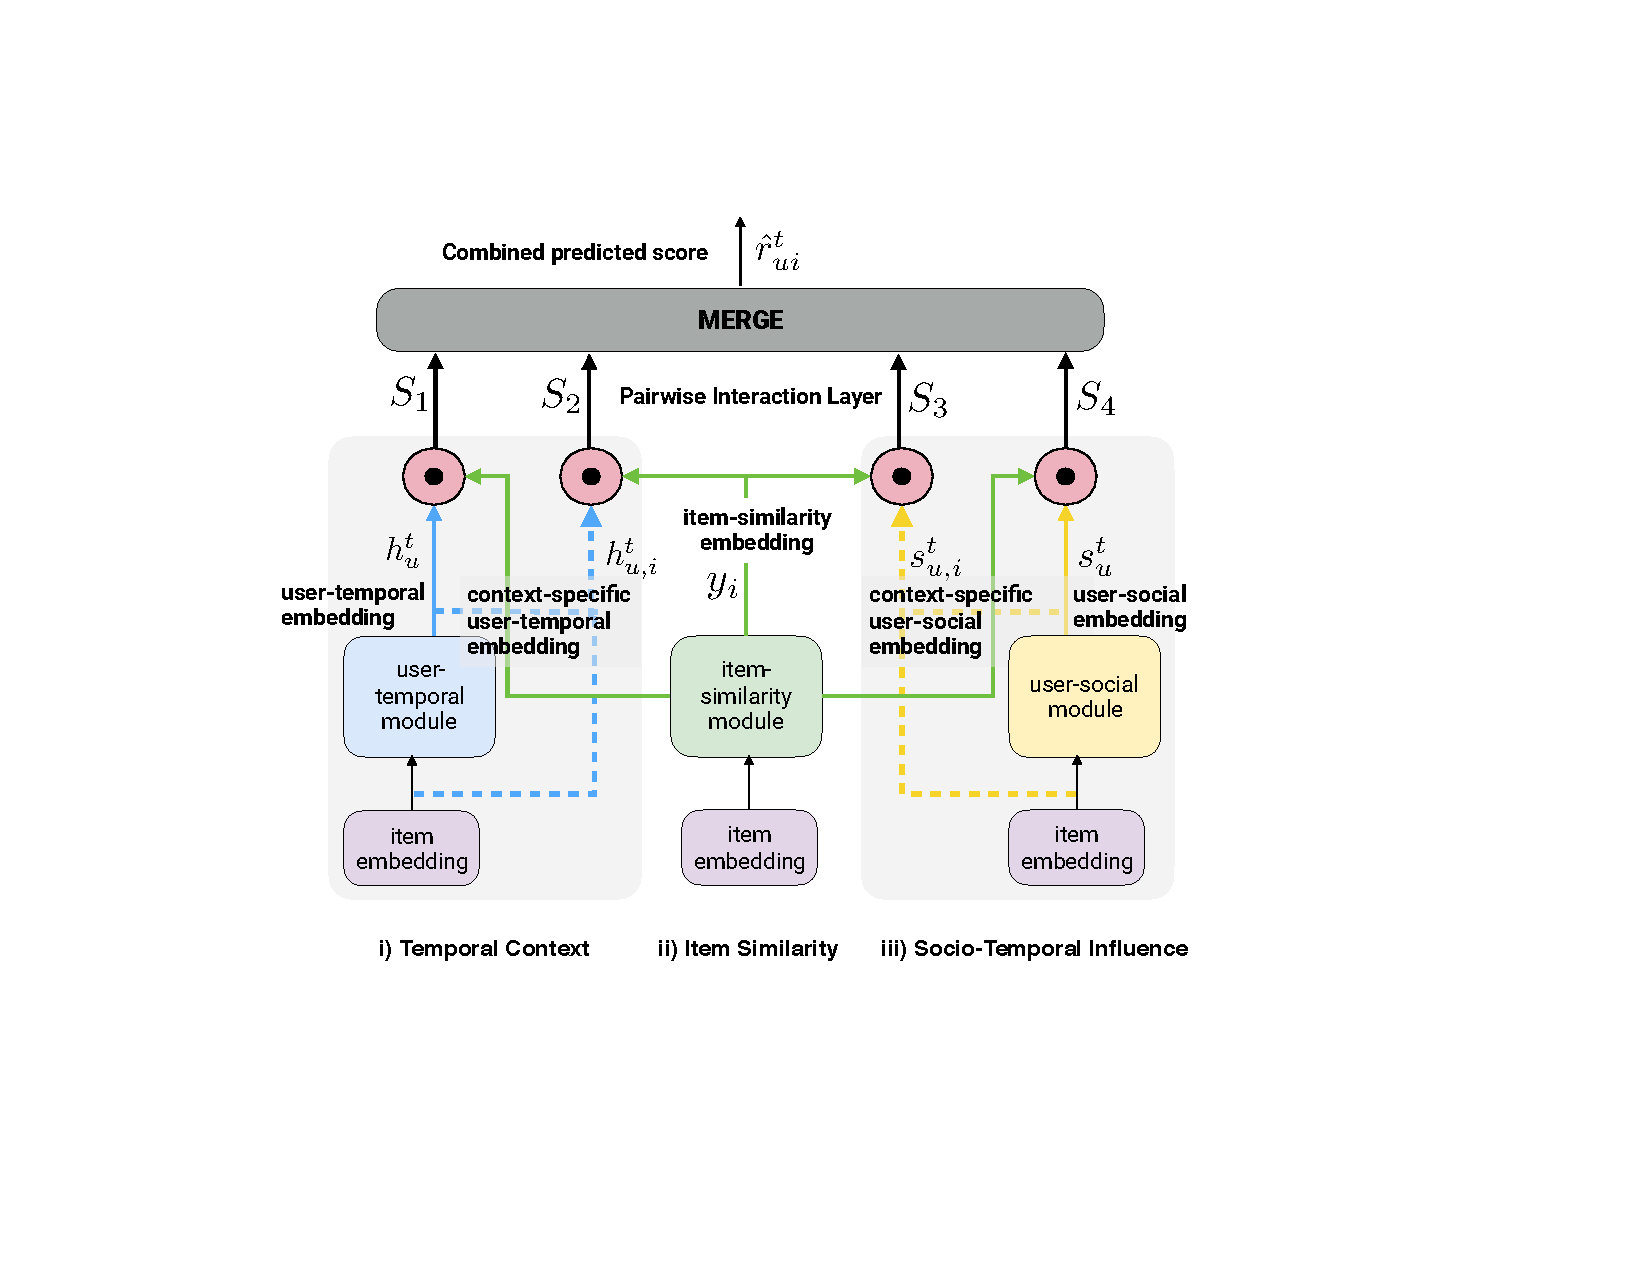
\includegraphics[width=0.7\textwidth]{figures/Overall_new}
  \caption{Overview of the proposed \ours {} model.  Our model computes pairwise interaction scores which compares item embeddings from the item-similarity module with user embeddings from both the user-temporal module and the user-social module. These scores are then merged using learnable weights to compute the final predicted score.
  }
  \label{fig:overview}
\end{figure}

As illustrated in Figure~\ref{fig:overview}, we obtain the  scores $S_k$ by combining information from the following three modules:
(1) the user-temporal module which leverages temporal information about a user;
(2) the user-social module which captures information about the recent interactions of a user's friends; and
(3) the item-similarity module, which captures information about item homophily.

Specifically, Eq.~\eqref{eq:fuse} combines four  pairwise interactions:
(1) $S_1 = h_u^{t} \cdot {y}_i$,
(2) $S_2 = h_{u, i}^{t} \cdot {y}_i$,
(3) $S_3 = s_u^{t} \cdot {y}_i$, and
(4) $S_4 = s_{u, i}^{t} \cdot {y}_i$.
Hereby, $\cdot$ indicates an inner product between two embeddings.
Note, all pairwise interaction scores $S_k$ assess the similarity between a $D$-dimensional representation obtained from the item-similarity module (${y}_i\in\mathbb{R}^D$) and information obtained from either the user-temporal module ($h_u^{t} , h_{u,i}^{t}\in\mathbb{R}^D$) or the user-social module ($s_u^{t} , s_{u,i}^{t}\in\mathbb{R}^D$).

The user-temporal module encapsulates information from a history of user interactions. This module computes a time-dependent embedding $h_u^t$ for user $u \in {\mathcal U}$ at time $t$. This embedding denotes a user's current preferences in general. We also compute a context-specific user-temporal  embedding, $h_{u,i}^t$ which encodes similarity of a user's current preferences ($h_u^t$) in the context of the candidate item $i \in {\mathcal I}$. Note that both embeddings capture different aspects (general and item specific) and are time-dependent.

The user-social module captures a user's social preferences based on the recent history of the user's social graph. Specifically, for user $u$ at time $t$, we encode this information in an embedding referred to as user-social embedding, $s_u^t$. Similar to the user-temporal module, we also compute a context-specific user-social embedding for a user, $s_{u,i}^t$, encoding similarity of a user's social preferences ($s_u^t$) with respect to the candidate item $i$.


The item-similarity module employs item-item collaborative filtering, building an implicit similarity network between items based on their features and co-occurrence in the dataset.
This module computes an item-similarity embedding ${y}_i$ for item $i \in {\mathcal I}$, which is identical across time. We think this is a reasonable assumption as properties of items do not change over time\footnote{Experiments with time-sensitive item embeddings decreased accuracy of the reported results.}.

We will next provide details about
computation of the user-temporal embedding $h_u^t$, the context-specific user-temporal embedding $h_{u,i}^t$, a user-social embedding $s_u^t$, the context-specific user-social embedding $s_{u,i}^t$, and the item-similarity embedding ${y}_i$.

\begin{figure}[tbh]
  \centering
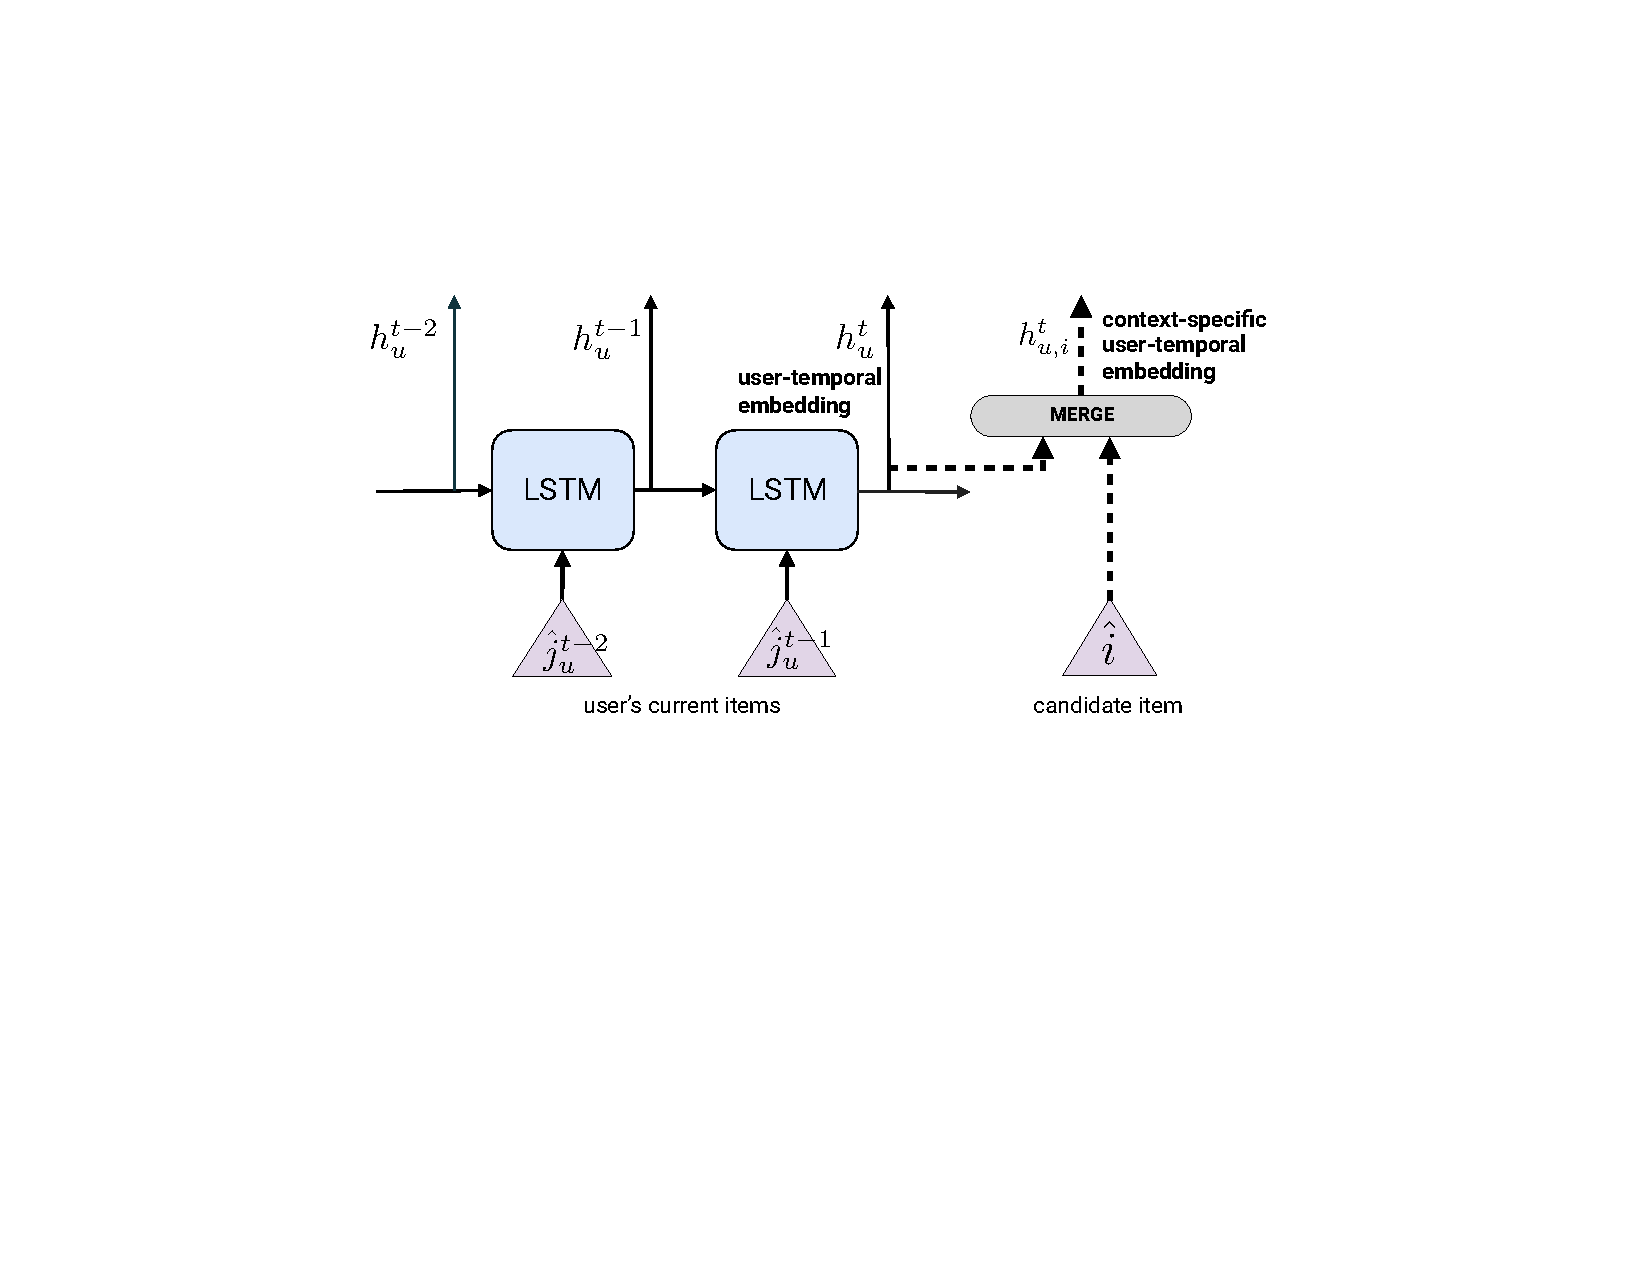
\includegraphics[width=0.7\textwidth]{figures/Temporal_new}
\caption{The user-temporal module uses an LSTM to compute an embedding $h_u^t$ based on a user's history $h_u^{t-1}$ and the current item $\hat{j}_u^{t-1}$. We also compute context-specific user-temporal embedding $h_{u,i}^{t}$ with respect to  candidate item $i$.}
\label{fig:temporal}
\end{figure}

\begin{figure*}[tbh]
\begin{subfigure}[c]{\linewidth}
\centering
  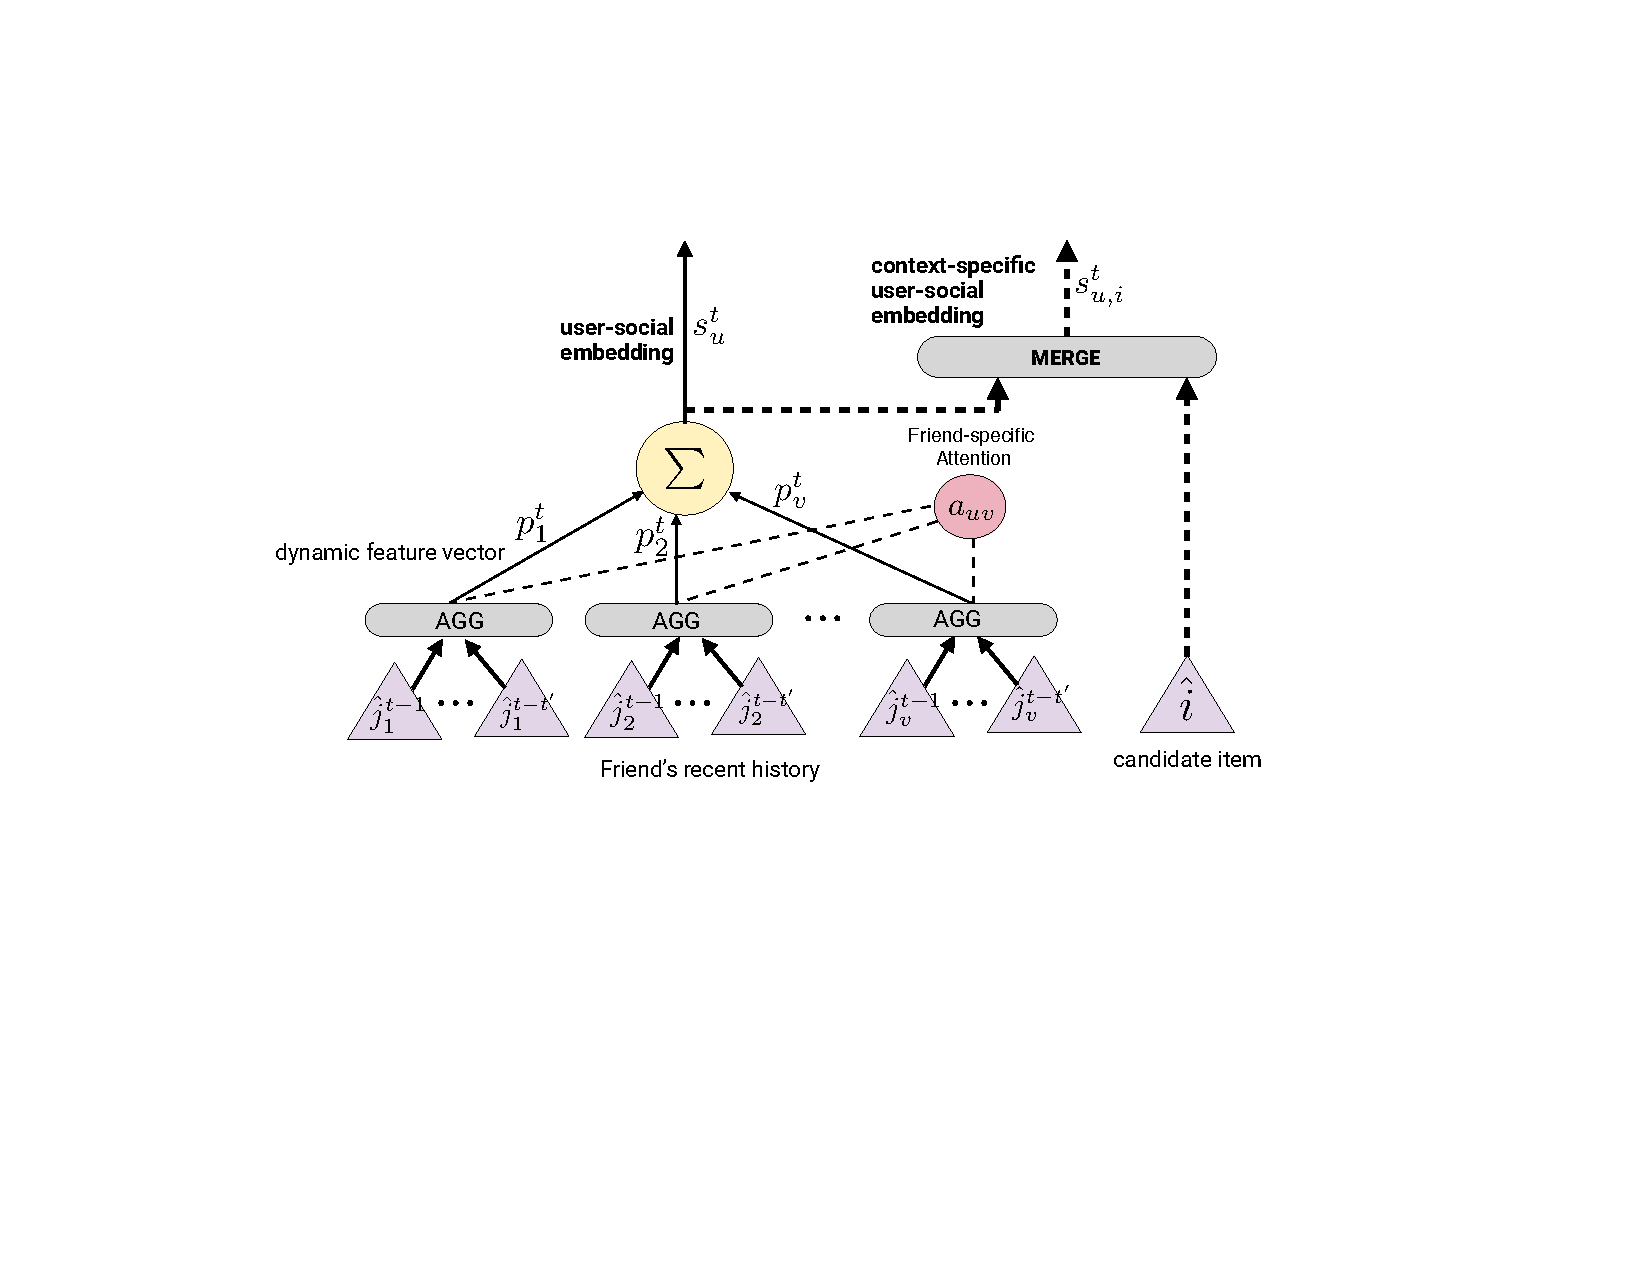
\includegraphics[scale=0.75]{figures/UserSocial_new}
  \label{fig:user}
\end{subfigure}
\caption{Illustration of the user-social module. The user-social module uses an attention based aggregation of the recent history of a user's social connections.}
\end{figure*}

\begin{figure*}[tbh]
\begin{subfigure}[c]{\linewidth}
\centering
  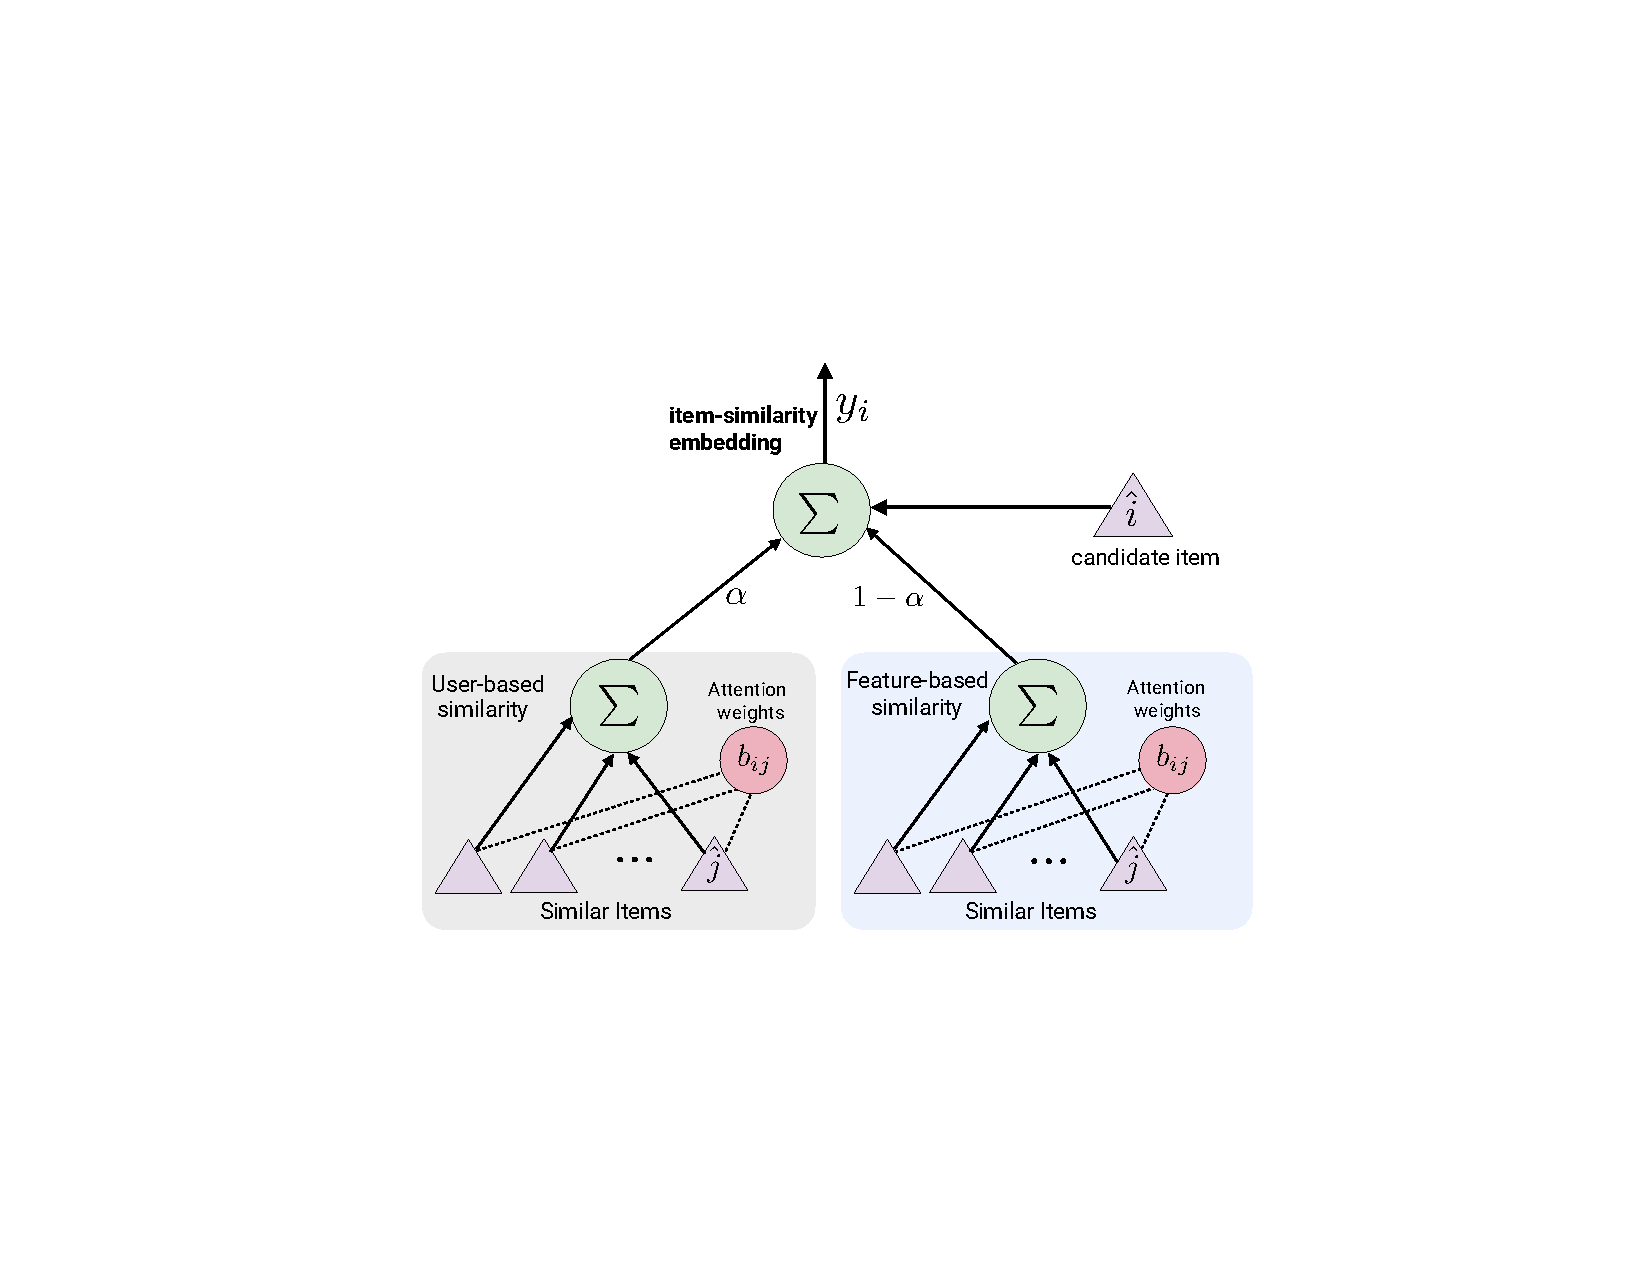
\includegraphics[scale=0.75]{figures/ItemModule_new}
  \label{fig:item}
\end{subfigure}
%\vspace{-0.2in}
\caption{Illustration of the item-similarity module. The item-similarity module aggregates embeddings from similar items in an attention aware manner. The item graphs are constructed based on frequency of co-occurrence and feature similarity. The parameter $\alpha$ trades influence between both item social graphs.}
\end{figure*}

\subsection{User-Temporal Module}
Users constantly interact with items offered on online platforms, e.g., users rate or watch movies. Importantly, a user's preference does not remain constant and changes over time.
To model temporal dynamics, classical methods have explored Markov chains, attention networks and convolution networks~\cite{FPMC, SAS:2018, Caser}. However, these methods assume dependence on only recent history and  thus do not capture long term dependencies within user-item preferences. To address this concern, we  use recurrent neural nets (RNNs) based on long-short-term-memory (LSTM) components. Those are widely used in natural language processing to capture sequential dynamics \cite{recurrent}.

In general, RNNs are based on the following recurrence relation, where $h^{t}$ represents the hidden vector at time $t$, $x^t$ is the input at time $t$ and $w$ refers to learnable weights:
\begin{align}
  h^{t} &= f(h^{t-1},x^{t-1}, w).
\end{align}

To specialize to our case, consider again a platform where users watch movies.
Formally, for each user $u$ at time $t-1$, let $j_u^{t-1} \in {\mathcal I}$ be the item which user $u$ interacted with at time $t-1$.  To compute its item embedding $\hat{j}_u^{t-1}\in\mathbb{R}^D$ (throughout we use `$\hat\cdot$' to indicate embeddings), we concatenate the item $j^{t-1}_u$  with its one-hot category information $c(j^{t-1}_u) \in \{0,1\}^{|C|}$ and apply the linear transformation
\begin{align}
  \hat{j}_u^{t-1} &= W_p [ j_u^{t-1} \mid \mid c(j^{t-1}_u)] + b_p.
\end{align}
With slight abuse of notation $j_u^{t-1}$ also denotes the one-hot representation.
Here, $W_p$ and $b_p$ are trainable parameters and represent weight and bias of a linear layer, `$ \mid \mid $' represents the concatenation operation and $C$ is the total number of item categories. This item embedding $\hat{j}_u^{t-1}$ is used as an input for an LSTM module based RNN which computes the user-temporal  embedding $h_u^{t}$ via
\begin{align}
  h_u^{t} &=  f'(h_u^{t-1}, \hat{j}_u^{t-1}, w).
\end{align}
Here, $f'$ represents the LSTM recurrence relation. This final user-temporal representation encodes a user's past behavior.

While $h_u^t$ captures a user's current preferences in general, we also separately capture relevance of candidate item $i$ with respect to the user's current preferences. For instance, if the user is currently watching action movies, we should capture if the candidate action movie $i$ matches her preferences.
Thus, context-specific user-temporal  embedding $h_{u,i}^t$ encodes similarity between user-temporal  embedding $h_u^t$ and the candidate item embedding $\hat{i}$.  Specifically, to capture similarity between the user-temporal embedding and the item embedding,
we compute $h_{u,i}^t$ as
\begin{align}
  h_{u,i}^{t} &=  W_q[h_u^{t} \mid \mid \hat{i} \mid \mid h_u^{t} \otimes \hat{i}] + b_q,
\end{align}
where $\hat{i}$ is the embedding of candidate item $i$ and $\otimes$ represents an element-wise product of two vectors. $W_q$ and $b_q$ are learnable parameters. \Cref{fig:temporal} depicts the architecture of this user-temporal module.

\subsection{User-Social Module}
Beyond temporal changes, users are influenced by recent behavior or ratings of  trusted friends. Also, influences are not equal among all friends.
To model this heterogeneous social influence, we use an attention based aggregation of a user's friends recent past behavior.  \Cref{fig:user} shows our user-social module. Formally, for user $u$ at time $t$, the user-social embedding $s_u^{t} \in \mathbb{R}^D$ is computed as
\begin{equation}
  \label{eq:user}
  s_u^{t} = \sum_{v \in F(u)} a_{uv} p_v^t,
  \end{equation}
where $F(u)$ represents  social connections of user $u$, $a_{uv}\in\mathbb{R}$ is the attention weight for friend $v$ and $p_v^t \in \mathbb{R}^D$ is a feature vector representing the recent history of friend $v$.

Most of the social recommender systems \cite{SBPR, SERec, GBPR} employ a uniform weighting for all social friends when computing influence. However, we argue that this is sub-optimal, particularly for social media, where a user does not trust  all friends equally. Indeed, we think modeling of trust is particularly important for online platforms due to large social circles with  superficial acquaintance. Thus,
we obtain the attention weights $a_{uv}$ from an influence score $e(u, v)$ for each user $u$ and friend $v$:
\begin{equation}
  e(u,v) = \text{LeakyReLU}(W_q [\hat{u} \mid \mid \hat{v}] + b_q),
  \end{equation}
where $\hat{u}, \hat{v} \in \mathbb{R}^D$ are user embeddings for user $u$ and $v$ respectively, while $W_q$ and $b_q$ are learnable parameters. The  attention weight $a_{uv}$ is  obtained by normalizing the influence score via a soft-max:
\begin{equation}
  a_{uv} = \frac{\exp(e(u,v))} {\sum_{v \in F(u)} \exp(e(u,v))}.
  \end{equation}

Each friend $v$ is represented by a dynamic feature vector $p_v^t$ which captures recent past behavior and is computed via
\begin{align}
  \label{eq:useragg}
  \hat{j}_v^{t'} &= W_r [ j_v^{t'} \mid \mid c(j_v^{t'})] + b_r, \\
  p_{v}^{t} &= \operatorname{AGG}(\{\hat{j}_v^{t'} \mid t' < t \}).
\end{align}
Here $\hat{j}_v^{t'} \in \mathbb{R}^D$ is the item embedding for item $j_v^{t'}$ clicked by user $v$ at time $t'$. Each past item rated by the friend before the current timestamp $t$ can be used to compute the historical profile of  friend $v$. In practice, we found that using the recent past gives similar performance compared to using all previous items. Therefore, we consider only the last $t'$ items of each friend. We aggregate these historical item embeddings using the mean aggregation operation $\operatorname{AGG}$. Note that
it is possible to aggregate this information in multiple ways but mean aggregation performed well in our experiments. It is also worthwhile to note that attention weights remain static across time while a user's feature vectors are dynamic.

Similar to the user-temporal module, we also compute a context-specific user-social embedding $s_{u,i}^t$. This embedding captures similarity of the user's social preferences with respect to the candidate item $i$. Formally,
\begin{align}
  s_{u,i}^{t} &=  W_s[s_u^{t} \mid \mid \hat{i} \mid \mid s_u^{t} \otimes \hat{i}] + b_s,
\end{align}
where $\hat{i}$ is the item embedding of candidate item $i$ and $\otimes$ is the element-wise product.

\subsection{Item-Similarity Module}
Online platforms operate with a large set of items, many of which are rated infrequently. It is consequently hard to construct meaningful representations of items, particularly if available information is scarce. Also, users are similarly attracted to related items but it is non-trivial  to implicitly learn item-item similarity.
To address this concern, we propose to construct a similarity aware item embedding based on information available for users which have interacted, e.g., clicked this item, and item features like category information.  \Cref{fig:item} illustrates our item-similarity module.

In particular, we represent each item $i \in {\mathcal I}$ via an n-hot vector $g_i \in \{0,1\}^{\vert \mathcal{U} \vert}$, where $n$ is the number of users who have interacted with item $i$ while $\vert \mathcal{U} \vert$ is the total number of users on the platform.  We then compute $k$-nearest neighbors for each item using cosine similarity between these n-hot vectors. This results in an implicit social network for item $i$, denoted by $F(i)$. All these items are similar as the same users interacted with them.
However, this approach of computing similarity between items is biased towards popular items with high user degree. Thus, we construct another item similarity network based on item features. In particular, we compute the  network $F' (i)$ based on items which belong to the same category.
We randomly connect $k'$ items of the same category in $F'(i)$. In our experiments, we let $k = k' $, i.e., we use the same neighborhood size for both  item networks.

We then  aggregate both of these item  graphs to learn item-similarity embeddings via
\begin{align}
  \label{eq:item}
y_i = \alpha \sum_{j \in F(i)} b_{ij} \hat{j} + (1-\alpha)\sum_{j \in F'(i)} b_{ij} \hat{j} + \hat{i},
\end{align}
where $\alpha\in[0,1]$ is a learnable parameter which controls the effect of co-occurring similarity versus category relationship. To compute the attention weights $b_{ij}$, we follow our earlier approach:
similar to the user model, $e(i, j)$  is the influence score for each item $i$ and its similar item $j$:
\begin{equation}
  e(i,j) = \text{LeakyReLU}\left ( W_n\lbrack \hat{i} \mid \mid \hat{j} \rbrack + b_n \right),
  \end{equation}
where $\hat{i}, \hat{j}$ are item embeddings for item $i$ and $j$ respectively, and $W_n$ and $b_n$ are learnable parameters. The final attention weight is obtained by normalizing the influence score via a soft-max function:
\begin{equation}
  b_{ij} = \frac{\exp(e(i,j))} {\sum_{j \in F(i)} \exp(e(i,j))}.
  \end{equation}
Note that we use the same embeddings to compute attention weights for both graphs.

The final estimated `item-similarity' module models similarity between items with similar features and frequently co-occurring items. This helps to address the data sparsity in the item space by exploiting item homophily.


Each module learns separates factors which influence user choices in recommender systems. We fuse these factors via a linear operation as detailed in Eq.~\eqref{eq:fuse}.

\subsection{Training}
We train all the three modules jointly in a unified framework using the binary cross-entropy loss:
\begin{equation}
L_{\theta} = - \sum\limits_{(u,i,t) \in \mathcal{B}}r_{ui}^t \log \left( \hat{r}_{ui}^t \right) + \left ( 1-r_{ui}^t \right ) \log \left ( 1-\hat{r}_{ui}^t \right) ,
\end{equation}
where $\theta$ represents all the learnable parameters in the model and $\mathcal{B}$ is the currently sampled mini-batch.
Specifically, for each sample $(u,i,t) \in \mathcal{B}$, we also obtain user $u$'s friends, $F(u)$ along with the corresponding item graph of the item $i$, i.e., $F(i)$ and $F'(i)$.

As we are dealing with implicit feedback, we don't have any negative samples. Thus, in each iteration of the training process, for every observed user-item interaction at time $t$, $(u,i,t) \in \mathcal{B}$, we sample $m$ unobserved items for user $u$.
Similar to \citet{Song:2019}, we assign a weight of $1/m$ for each negative instance to provide a weak negative signal. This is done as each unobserved item does not necessarily mean that the user will not interact with this item in the future. For our experiments, we set $m=5$.

\noindent
\textbf{Parameter Settings.}
For all three modules, we use an embedding size $D = 32$ for all user and item embeddings. We also initialize the embedding matrix using a Gaussian distribution with a mean of 0 and a standard deviation of $0.01$. For the user-social and item-similarity modules, in each iteration, we subsample a set of friends $F$ at each timestamp for a user (item) instead of considering all friends. This sampling has two benefits: (1) it avoids overfitting by introducing random noise in the social module; and (2) it is computationally more tractable. We use a sample size of 10 for both user $F(u)$ and item $F(i), F'(i)$ social graphs. If a user has less than 10 friends, we pad the remainder with zeros. We set a friend's past history length, $t' =  3$ in the user-social module. We will study the effect of this  and other hyper-parameters subsequently.

For the user-temporal and user-social module, we set the length of the historical sequence of user interactions to $30$ for all users. For users with history length less than $30$, we utilize all the available interactions.
We also study the effect of this sequence length on our results in the next section.
We use the Adam optimizer for training our model and perform a grid search over \{0.1, 0.01, 0.001\} for a suitable learning rate on the validation set. We report results on the test set for the best performance model on the validation set. We also use dropout along with gradient clipping with a value of 0.25 and L2 regularization on the user and item embeddings to avoid overfitting.

% !TEX root = SADR.tex
\section{Experiments}
In this section, we first describe the datasets we use to evaluate the proposed approach, followed by the evaluation setup and competing state-of-the-art baselines. We then analyze the performance of our model, followed by ablation studies on different modules and hyper-parameters. Finally, we analyze the importance of each module using the learned weight parameters.

\subsection{Datasets}
We use benchmark datasets available from three online social review platforms: Ciao, Epinions, and CiaoDVD.

Ciao is a product review website where users provide reviews along with ratings for products ranging across a variety of categories. This dataset was crawled by Tang et al.~\cite{Tang} and contains rating information along with the creation timestamp given up to May 2011. Users also establish directed trust relations with other users on the platform and add them to their 'Circle of Trust.'
Epinions is another popular online consumer review website like Ciao~\cite{Tang}. However, this dataset is longer spanning a decade from Aug.\ 1999 to Nov.\ 2013. This dataset also contains trust relations between users\footnote{Both Ciao and Epinions datasets are available at www.cse.msu.edu/~tangjili/trust.html}.
CiaoDVD is a movie review dataset of DVDs crawled from \url{dvd.ciao.co.uk} in December 2013. This dataset contains user reviews of movies accompanied by their overall rating. It also contains directed trust relations between users\footnote{Dataset available from \url{www.librec.net/datasets.html}}.

\begin{table}[tbh]
  \centering
\begin{tabular}{l r r r r } \toprule
  Dataset & \#users & \#items  & \#ratings & \#trusts\\ \hline
 Ciao & 1,653  & 16,862 & 26,190 & 32,955 \\
 Epinions&  22,143  & 296,278 & 464,249 & 83,363 \\
 CiaoDVD & 2,609  & 16,122 & 32,054 & 8,926 \\\bottomrule
\end{tabular}
\vspace{-0.1in}
  \caption{Dataset statistics.}
\label{tab:data}
\end{table}

As we are dealing with implicit feedback (user-item interaction data), we convert all the observed interactions, i.e., ratings, into positive instances. For both datasets, we only keep users with at least five rated items. The final data statistics are summarized in Table~\ref{tab:data}. Epinions is by far the largest dataset.

%-------------------------------------------------------------------------
\subsection{Evaluation Protocol}
We split each user sequence into training, validation, and test set. For each user, the most recent item is held out for testing. The second most recent item is held out for validation while we train the model on the remainder of the sequence. The validation set is used for tuning the model hyper-parameters, e.g., learning rate, embedding dimension, sample size of user's friends, etc. % of the model.

We evaluate model performance on the test set via two widely used evaluation metrics:  HitRate@10 (HR@10) and Area under Curve (AUC). HitRate@10 is computed as follows:
\begin{align}
  HR@10 = \frac{1}{\vert {\mathcal U} \vert} \sum_{u \in {\mathcal U}} \mathbbm{1}  (L_{u,i_u^{t}} < 10),
\end{align}
where $i_u^{t}$ is the ground truth item that user $u$ clicked at test time $t$, $L_{u,i_u^{t}}$ is the rank of the ground truth item in the predicted ranked list, and  $\mathbbm{1}(.)$ is the indicator function. The HR@10 metric checks if the ground truth item is present in the top-10 ranking.
In contrast, AUC measures the rank of the test item in the predicted ranked list. This is a harder metric as it takes into account  the exact position of the ground truth item. Formally,
\begin{align}
AUC = \frac{1}{\vert {\mathcal U} \vert} \sum_{u \in {\mathcal U}} \frac{1}{\vert {\mathcal I} \vert} \sum_{j \in {\mathcal I}} \mathbbm{1} (L_{u, i_u^{t}} > L_{u,j}).
\end{align}
where $L_{u,j}$ is the rank of item $j$ in the predicted ranked list for user $u$.
Due to the sparsity of user-item interaction data (number of items is huge) and computational feasibility, following~\cite{He:2016}, HitRate@10 is reported on a sample subset of negative items instead of the whole set. For each user-item pair in the test set, we sample 99 negative items that the user has not rated before.  Similarly, for AUC computation, we sample a set of 5,000 unobserved items for each user for both our model and the baselines.

\subsection{Baselines}
We compare to a large variety of state-of-the-art collaborative filtering (CF), temporal, social, and socio-temporal recommenders:
\begin{itemize}
\item BPR-MF~\cite{Rendle} is a classic matrix factorization model which uses a pairwise ranking loss.
\item NeuMF~\cite{NeuMF} is a recently proposed CF based model with neural architecture. It merges matrix factorization and multi-layer perceptron modules to predict item ranking.
\item NAIS~\cite{NAIS} is an item-to-item CF based model which employs user-specific attention between items to identify similar items\footnote{\url{github.com/AaronHeee/Neural-Attentive-Item-Similarity-Model}}.
\item TBPR~\cite{TBPR} extends the BPR model to capture strong and weak ties separately in a user's social network in order to distinguish the degree of influence of a user's connections on her behavior.
\item SERec~\cite{SERec} is a state-of-the-art CF based social recommender model that augments collaborative filtering with social exposure through regularization and boosting.
\item DiffNet~\cite{Diffnet} is a state-of-the-art graph convolution based social recommender that propagates user influence through their social network. Due to the absence of attributes in our dataset, we replace the user and item feature vectors with one-hot embeddings in their model\footnote{\url{github.com/PeiJieSun/diffnet}}.

\item GraphRec~\cite{fan2019} is another recently proposed social recommender that uses graph convolution networks to incorporate information from both a user-item and a user's social graph.
The original model was proposed for rating prediction, and we adopt it for our item ranking task. For that purpose, we change the loss function to a log loss and augment the training data with randomly sampled negative items following other ranking prediction models \cite{NeuMF}.

\item SASRec~\cite{SAS:2018} is a state-of-the-art model for the temporal recommendation that uses a self attentive module to capture long-term interests of a user\footnote{\url{github.com/kang205/SASRec}}.

\item SR-GNN~\cite{SRGNN} is a graph neural network based temporal recommender that aggregates information from all previous timesteps of the user\footnote{\url{github.com/CRIPAC-DIG/SR-GNN}}.

\item SPMC~\cite{Cai:2017} is an extension of a Markov chain based~\cite{Rendle2} model which captures both temporal and social dynamics for recommendation\footnote{\url{github.com/cwcai633/SPMC}}.


\item ARSE~\cite{Sun:2018} is a state-of-the-art social session recommendation model. It employs a session LSTM module to model change in user preferences across sessions while incorporating social influence as an input to the LSTM module\footnote{\url{github.com/DeepGraphLearning/RecommenderSystems/}}. Similar to their paper, we divide the dataset into monthly intervals and predicted for the next session\footnote{We also experimented with constraining each session to comprise of just a single item, but that resulted in slightly worse performance.}.
\item DGRec~\cite{Song:2019}: Another social session recommender method that uses graph attention networks to merge preferences of social neighbors from the previous session with a user's preference in the current session. We use similar month-wise intervals to denote each session\footnote{We also evaluated other intervals, but they all performed similarly.}.
\end{itemize}

BPR-MF, NeuMF and NAIS are Collaborative Filtering models, while TBPR and SERec are social recommenders.
Diffnet and GraphRec are graph convolution based social recommenders. SASRec and SR-GNN are temporal recommender models. We omit a comparison with Fossil and GRU~\cite{GRU4Rec} as they are RNN based temporal recommendation methods. The results for our user-temporal module are equivalent to their models.
SPMC is most similar to our model as it also models temporal behavior and socio-temporal influence. However, it is a shallow model as it extends a Markov chain to model linear dependence. ARSE and DGRec are also socio-temporal recommenders proposed for session recommendations.

We use the Adam optimizer for our models with a batch size of 256 for Ciao, CiaoDVD, and 1024 for Epinions. We used the implementation provided by the RecQ python library\footnote{\url{github.com/Coder-Yu/RecQ}} for BPR-MF, NeuMF, TBPR, and SERec models. We used the authors' implementation for all the other models. Specifically, for ARSE and GraphRec, we wish to thank the authors as they generously shared their implementation.
We keep the embedding dimension $D=32$, for all the baselines to be comparable with our model. We report the best result of the baselines using either hyper-parameters based on the authors' specifications or values, which performed better on our validation set.

\subsection{Performance Analysis}

Table~\ref{tab:baseline} details a comparison of HR@10 and AUC for our model and the state-of-the-art baselines on all three datasets. We report mean results over five runs.
Our model significantly outperforms all the baselines on the AUC metric by at least around 2\% for CiaoDVD, 14\% for Epinions, and 18\% for Ciao.
On the Ciao and Epinions dataset, our \ours {} model also improves the HR@10 metric by at least 4\%. Note that each of the baselines models one or a subset of three factors (temporal, socio-temporal, and item similarity), while our \ours {} model considers all factors jointly. Each of our modules outperforms their respective baselines. Further, the combined \ours {} model considerably outperforms the individual components. This improvement indicates that our model is effective at combining the individual modules, each capturing a distinct factor affecting a user's preference.

\begin{table*}[tbh]
  \centering
  \setlength{\tabcolsep}{5pt}
\begin{tabular}{p{34mm} l c c c c c c} \toprule
\multirow{2}{*}{Model Type}  & \multirow{2}{*}{Models} & \multicolumn{2}{c}{Ciao} & \multicolumn{2}{c}{Epinions}  & \multicolumn{2}{c}{CiaoDVD}\\
    &    &  HR@10   &    AUC         &    HR@10   & AUC &    HR@10   & AUC \\ \hline
  \multirow{3}{*}{Classical} & BPR-MF~\cite{Rendle} & 0.297 & 0.630 & 0.509 & 0.731 & 0.517 & 0.759 \\
   & NeuMF~\cite{NeuMF}  & 0.342 & 0.570 & 0.470 & 0.709 & \textbf{0.551} & 0.760 \\
   & NAIS~\cite{NAIS}  & 0.241 & 0.626 & 0.510 & 0.723 & 0.487 & 0.742 \\ \hline
  \multirow{4}{*}{Social} & SERec~\cite{SERec} & 0.295 & 0.550 & 0.421 & 0.613 & 0.385 & 0.647 \\
  & TBPR~\cite{TBPR}  & 0.322 & 0.601 & 0.47 & 0.717 & 0.518 & 0.745 \\
  & DiffNet ~\cite{Diffnet}  & 0.342 & 0.583 & - & - & 0.527 & 0.759 \\
  & GraphRec~\cite{fan2019}  & 0.234 & 0.534 & 0.452 & 0.702 & 0.33 & 0.708 \\
  \hline
\multirow{2}{*}{Temporal} & SASRec~\cite{SAS:2018} & 0.324 & 0.575 & 0.508 & 0.724 & 0.546 & 0.761 \\
  & SR-GNN~\cite{SRGNN} & 0.320 & 0.590 & 0.509 & 0.732 & 0.546 & 0.759 \\ \hline
\multirow{3}{*}{Social + Temporal}  & SPMC~\cite{Cai:2017} & 0.223 & 0.599 & 0.483 & 0.717 & 0.53 & 0.758 \\
& ARSE~\cite{Sun:2018} & 0.328 & 0.583 & 0.522 & 0.726 & 0.527 & 0.754 \\
& DGRec~\cite{Song:2019} & 0.329 & 0.610 & 0.479 & 0.726 & 0.521 & 0.753 \\ \hline
  \multirow{3}{*}{Our Indiv. Modules}  & User-Temporal & 0.308 & 0.666 & \textbf{0.559} & 0.726 & 0.535 & 0.751 \\
    & User-Social & 0.344 & 0.637 & 0.503 & 0.736 & 0.551 & 0.741 \\
  &Item-Similarity & 0.208 & 0.604 & 0.430 & 0.758 & 0.474 & 0.767 \\ \hline
Ours Combined  & \ours & \textbf{0.355} & \textbf{0.745} & 0.549 & \textbf{0.834} & 0.538 & \textbf{0.774} \\
 \bottomrule
\end{tabular}
  \caption{Comparison of results of our model to state-of-the-art baselines and variants of our own model on three datasets. Higher values are better for both metrics. Our model significantly outperforms the baselines that model a subset of three factors. `$-$' indicates an out of memory error.
  }
\label{tab:baseline}
\end{table*}

Amongst our proposed modules, in general, the user-social module performs best on the HR@10 metric, while the item-similarity module outperforms the other modules on the AUC metric. This difference could be because the user-social module improves the ranking of items currently popular among a user's social connections.
In contrast, the item-similarity module emphasizes items that frequently co-occur in the entire dataset, irrespective of the user preferences. This increases the bias of the item ranking only slightly, as co-occurrence is a weak signal for a specific user (it is averaged across all users).
This difference further underlines that it is essential to model a variety of factors for an effective recommendation.

\textbf{Collaborative:} CF-based approach BPR-MF performs the best among the baselines when considering the AUC metric while NeuMF performs competitively for HR@10.
This superior performance highlights that classical matrix factorization approaches are still very competitive for the recommendation. The user-specific attention-based NAIS model did not outperform the non-attention based CF models.

\textbf{Social:} Our proposed user-social module outperforms all baseline social recommenders for both metrics.
Among the baselines, the TBPR model that models the user's social graph with different weights for strong and weak ties performs better than the SERec that considers each friend's contribution equally. This reaffirms our assumption that each friend exerts a different influence on the user. In general, we found the recently proposed SERec to underperform on the three datasets used here. It proposes that social connections have a limited influence on a user's preference.  Social influence is weakly modeled through an exposure prior on the items. However, we think the low performance indicates the contrary, i.e., social influence plays a significant part in shaping a user's preference.

Our GCN based user-social module is inherently different from the other GCN based baselines, DGRec, and GraphRec. Our user-social module is time-dependent with dynamic user features while both baselines operate on static features (entire item history). Further, our architecture differs: we employ attention between a user and her social connections, whereas DiffNet does not use attention, and GraphRec computes attention based on user history rather than the user itself. Our superior performance supports the difference.

However, the DiffNet model performs the best among social recommenders. However, it is unable to scale to our largest dataset, Epinions. Note that we used the authors' implementation, and our largest dataset is bigger than the one reported in their paper. In contrast, the other GCN based model GraphRec performs poorly on all the datasets. Note that for results obtained in their paper, they only consider users with non-zero social connections and items previously seen in the training data, while we do not make any such assumptions.

\textbf{Temporal:} Our user-temporal module uses information from only the previous timestep for prediction at the current timestep while the baseline temporal recommenders aggregate information from all previous timesteps. However, we argue that information from a distant past is not useful. Comparable performance of our user-temporal module with the temporal baselines confirms our argument.
In general, both the temporal recommenders, SASRec and SR-GNN, perform better than social recommenders and are comparable to the best performing BPR baseline on the Epinions and CiaoDVD dataset when using the AUC metric. While they perform competitively with other baselines on HR@10.

\textbf{Social + Temporal:} SPMC, which combines temporal and social influence, performs worse than baselines, which model either of the two factors. This worse performance is expected as it is a shallow model with linear dependence. The other socio-temporal models ARSE and DGRec perform similarly, with ARSE performing slightly better for the HR@10 metric. Note that despite modeling socio-temporal influence, these methods do not outperform even other social and temporal only baselines. This could be since these models were originally proposed for the session-based recommendation. Sessions are typically defined as a sequence of activities performed by a user in a single visit to the website or platform.

Thus, for the session prediction settings, models work on recommending the next item to consume by the user in the same session. They typically assume either none or limited past session information of the users and assume static user preferences per session.
In contrast, we model the evolution per item for each user and expect a significant change in a user's preference over time.

Further, DGRec only models socio-temporal influence (based on a friend's last session) and ignores the evolution of a user's preference across sessions. In contrast, ARSE models a user's evolution across sessions but aggregates information per session resulting in limited flexibility. Also, it is worthy to note that none of these models exploit similarity in the item space that is used in our proposed model.
Thus, the worse performance of these session-based socio-temporal methods indicates that they are not well suited for temporal recommendation owing to information aggregation within sessions.

\subsection{Module Analysis}
\label{sec:mod}

\begin{figure}[tbh]
 \centering
   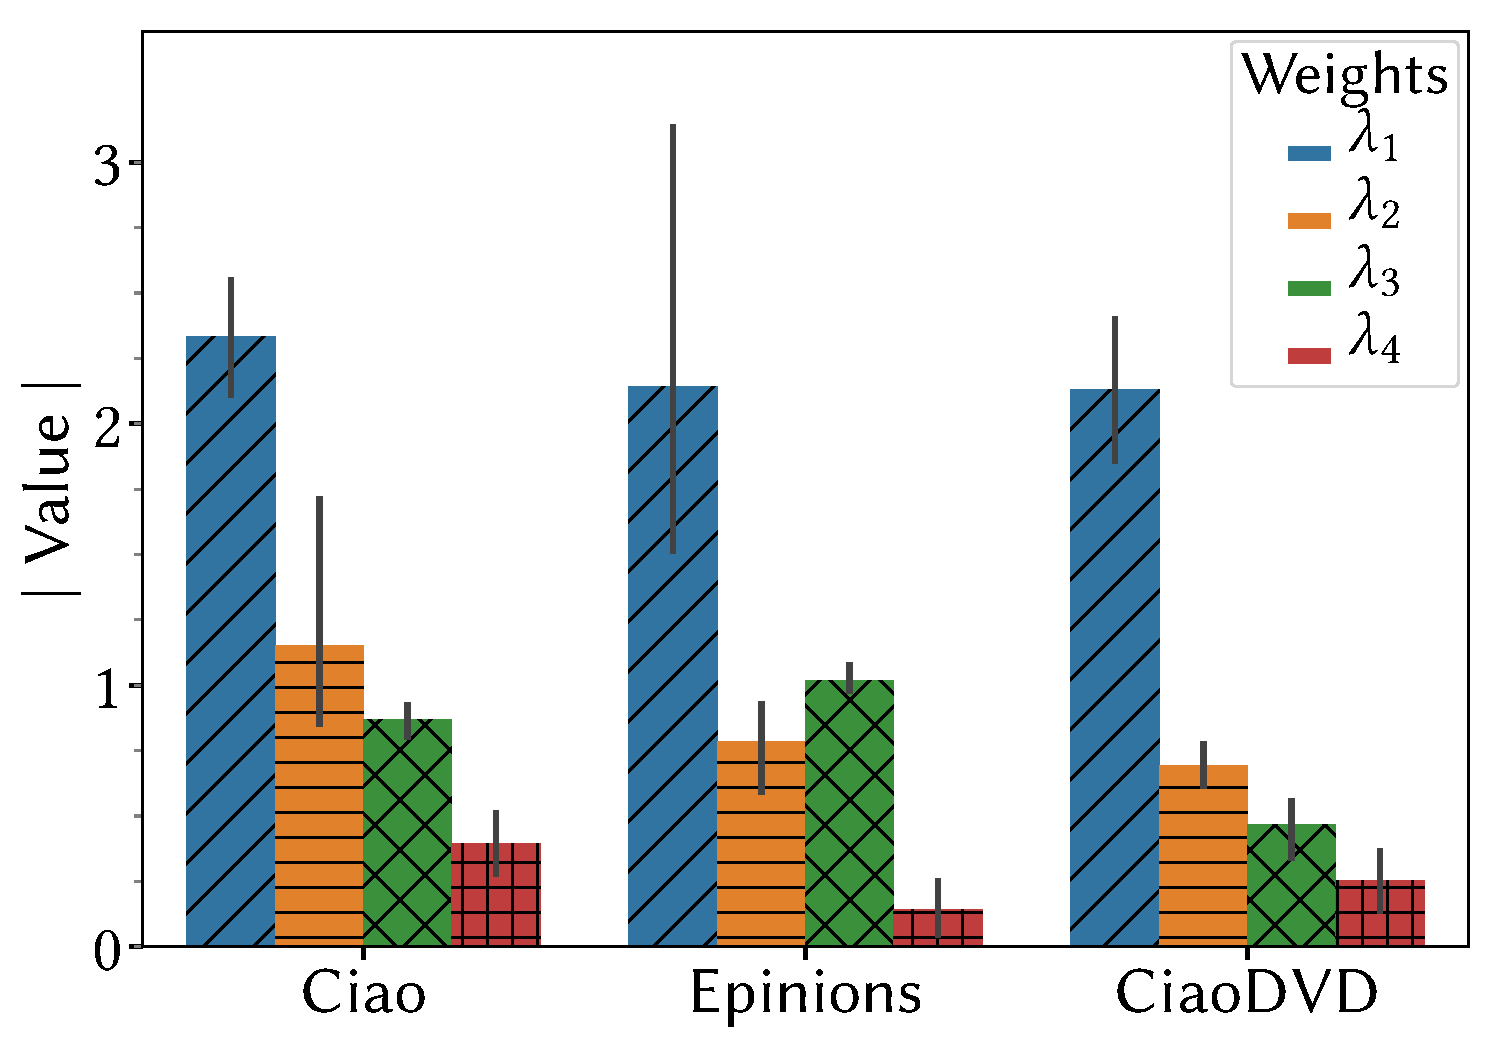
\includegraphics[scale=0.36]{figures/weight.pdf}
 \caption{Learned value of the weights $\lambda_k$ for $k \in \{ 1, \ldots ,4 \}$ for different scores in our model. Weight $\lambda_1$ corresponding to user-temporal embedding contributes most to the final score.}
 \label{fig:weight}
\end{figure}

We now evaluate the importance of each module (user-temporal, user-social, and item-similarity) in our combined model using learned weights, $\lambda_k$. \Cref{fig:weight} shows the learned magnitude of the weights $\lambda_k$ for $k \in \{ 1, \ldots ,4 \}$ for each of the $S_k$ (\Cref{eq:fuse}) scores for all the datasets. Weight $\lambda_1$ corresponds to a user-temporal embedding ($h_u^t$) %\as{`user temporal' or `temporal user'?}
and contributes most to the final score. This high magnitude is expected as a user's history of interactions play a crucial role in modeling user preferences accurately.
$\lambda_2$ corresponds to the context-specific user-temporal embedding ($h_{u,i}^t$) and is the second most important factor for Ciao and CiaoDVD datasets. In contrast, $\lambda_3$, which corresponds to a  user-social embedding ($s_{u}^t$) is the second highest factor for Epinions. This difference indicates that social influence plays an important factor for users in the Epinions dataset while it is slightly less important for the Ciao and the CiaoDVD datasets. $\lambda_4$, which  corresponds to the context-specific user-social embedding ($s_{u,i}^t$) contributes the least across all datasets. Note that all scores use item-similarity embeddings.

Next, we perform ablation experiments by removing each individual module at a time from the final model, as shown in \Cref{tab:individual}.
All variants perform worse than the final \ours {} model, emphasizing the need for each of the modules.
For all the datasets, removing the user-temporal module results in the largest drop in performance. This is expected as a user's history encapsulates a great deal of information for the recommendation. Thus, personalized recommendations fare better than generic ones.

\begin{table}[tbh]
  \centering
\begin{tabular}{l  c c c c c c} \toprule
\multirow{2}{*}{Model Variants} & \multicolumn{2}{c}{Ciao} & \multicolumn{2}{c}{Epinions} & \multicolumn{2}{c}{CiaoDVD} \\
&  HR@10   &    AUC         &    HR@10   & AUC &    HR@10   & AUC \\ \hline
\{social + item\} & 0.329 & 0.574 & 0.478  & 0.713 & 0.526 & 0.738\\
\{temporal + item\} & 0.335 & 0.631 & 0.557 & 0.798  & 0.531 & 0.743\\
\{temporal + social\} & 0.327 & 0.679 & 0.536 & 0.736  & 0.540 & 0.745\\
\ours & 0.355 & 0.745 & 0.549 & 0.834  & 0.538 & 0.774 \\
 \bottomrule
\end{tabular}
    \caption{Performance of our \ours {} model for all three datasets, when removing one module at a time. All of these variants perform worse  than the combined model.}
    \label{tab:individual}
\end{table}

Apart from the user-temporal module, for CiaoDVD, the model without the item-similarity module performs best, while for Epinions and Ciao, the model without user-social module performs the best. Thus, for the movie reviewing platform CiaoDVD, preferences of a user's social connections play a significant role in predicting her movie preferences.

In contrast, for Epinions and Ciao, both of which contain broad categories of products, items frequently bought together by users are better predictors of purchasing behavior. This seems intuitive as movie preferences are subjective in general, while users tend to believe strangers on online reviewing platforms for products like electronics, furniture, etc.


\begin{figure}[tbh]
  \centering
    \begin{tabular}{c c c c}
      item-similarity & user-social & user-temporal \\
    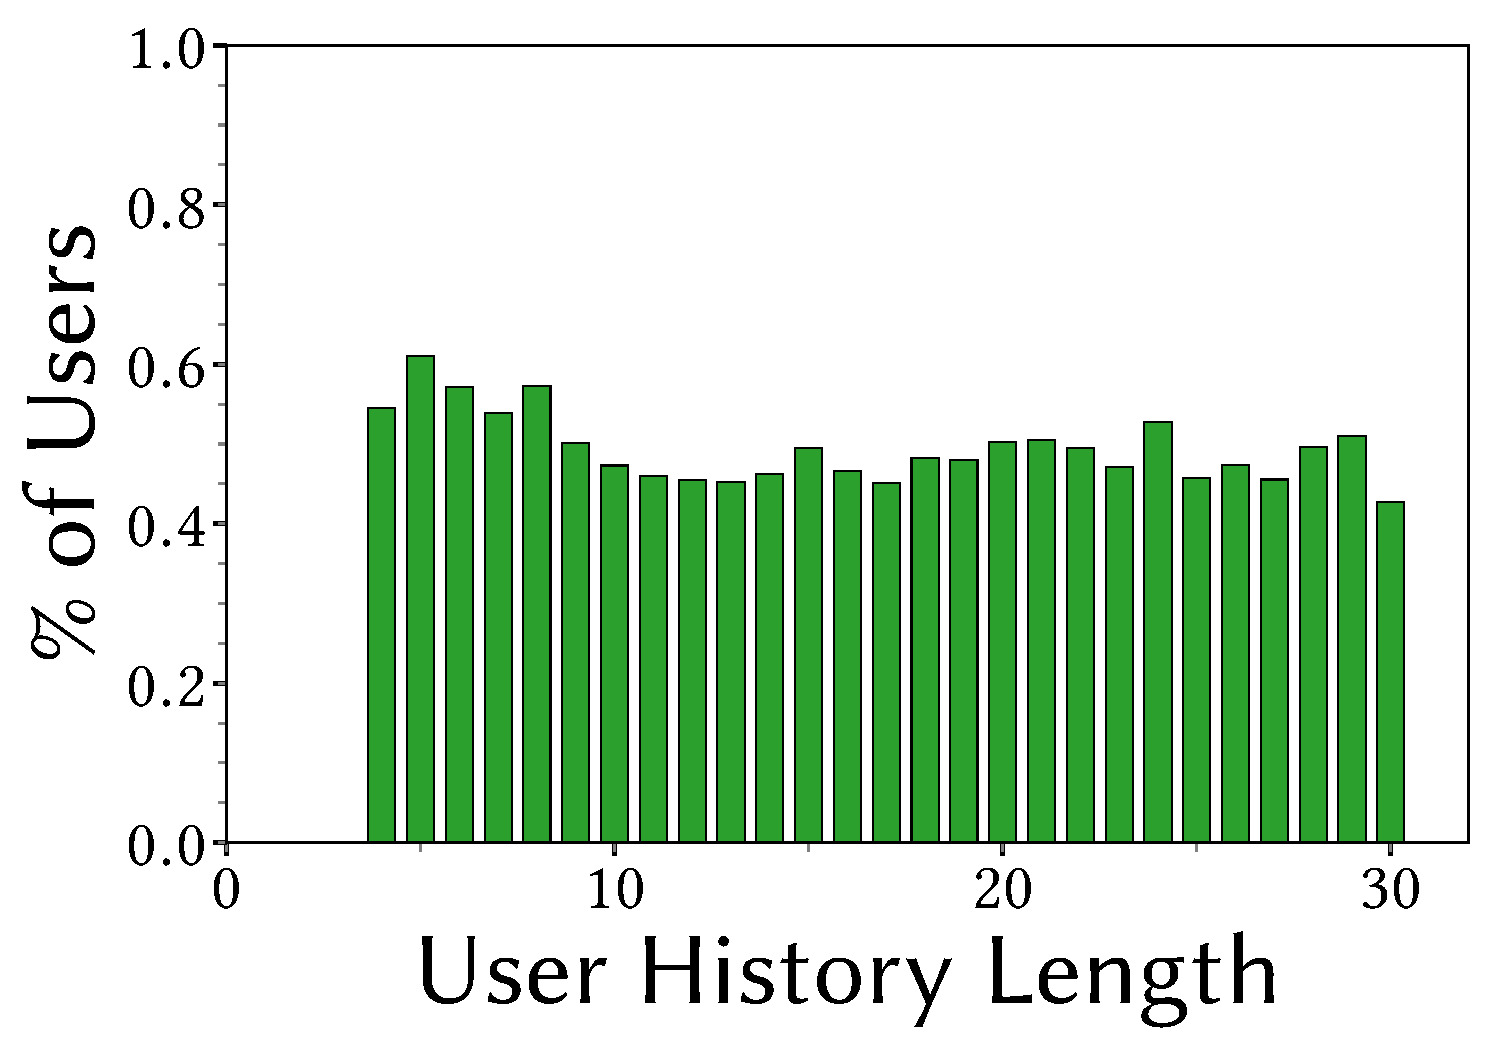
\includegraphics[height=4cm,width=0.3\linewidth]{figures/epinions_itemSocial_Total_users_length.pdf}
 &
    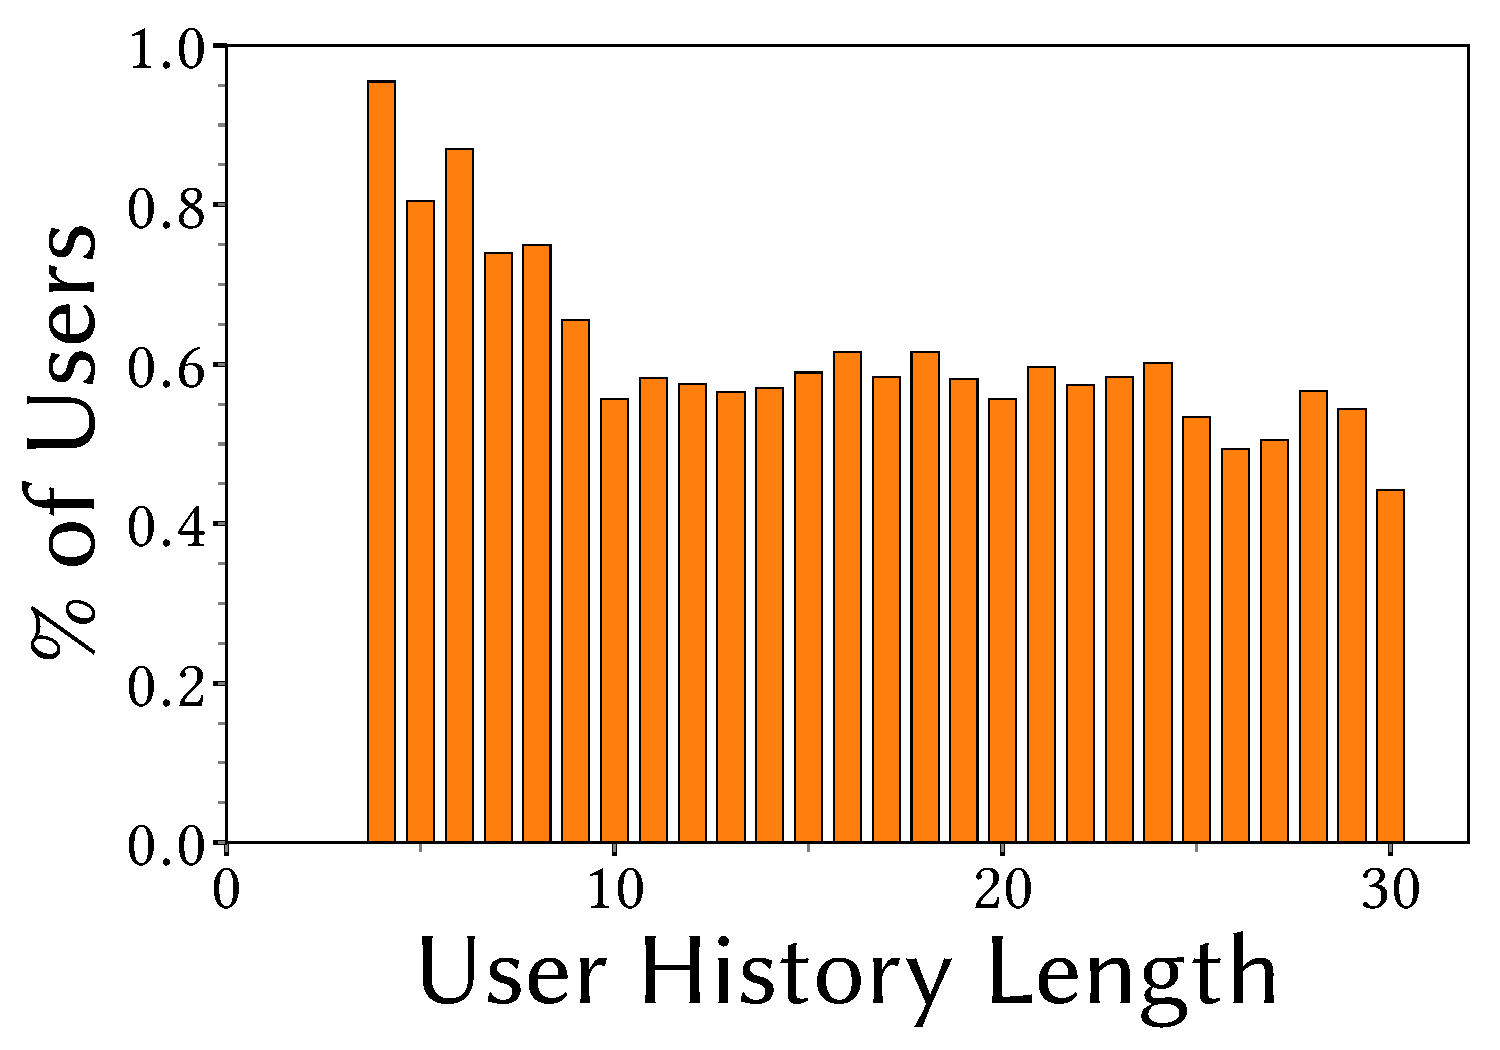
\includegraphics[height=4cm,width=0.3\linewidth]{figures/epinions_userSocial_Total_users_length.pdf}
  &
    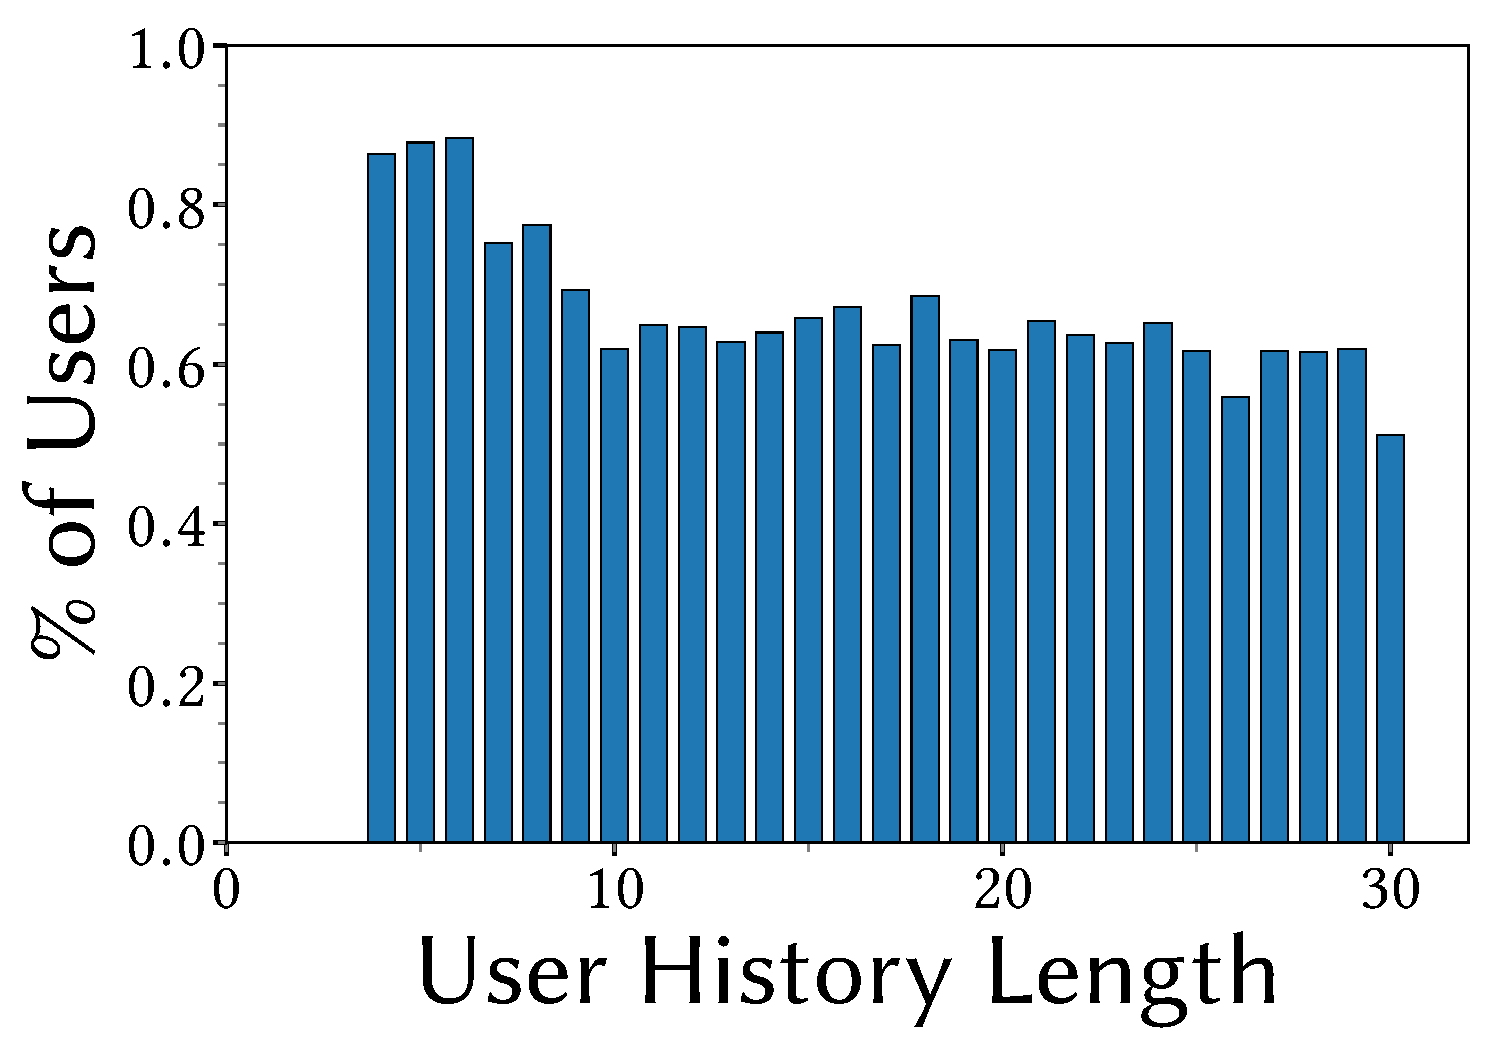
\includegraphics[height=4cm,width=0.3\linewidth]{figures/epinions_temporal_Total_users_length.pdf}\\
    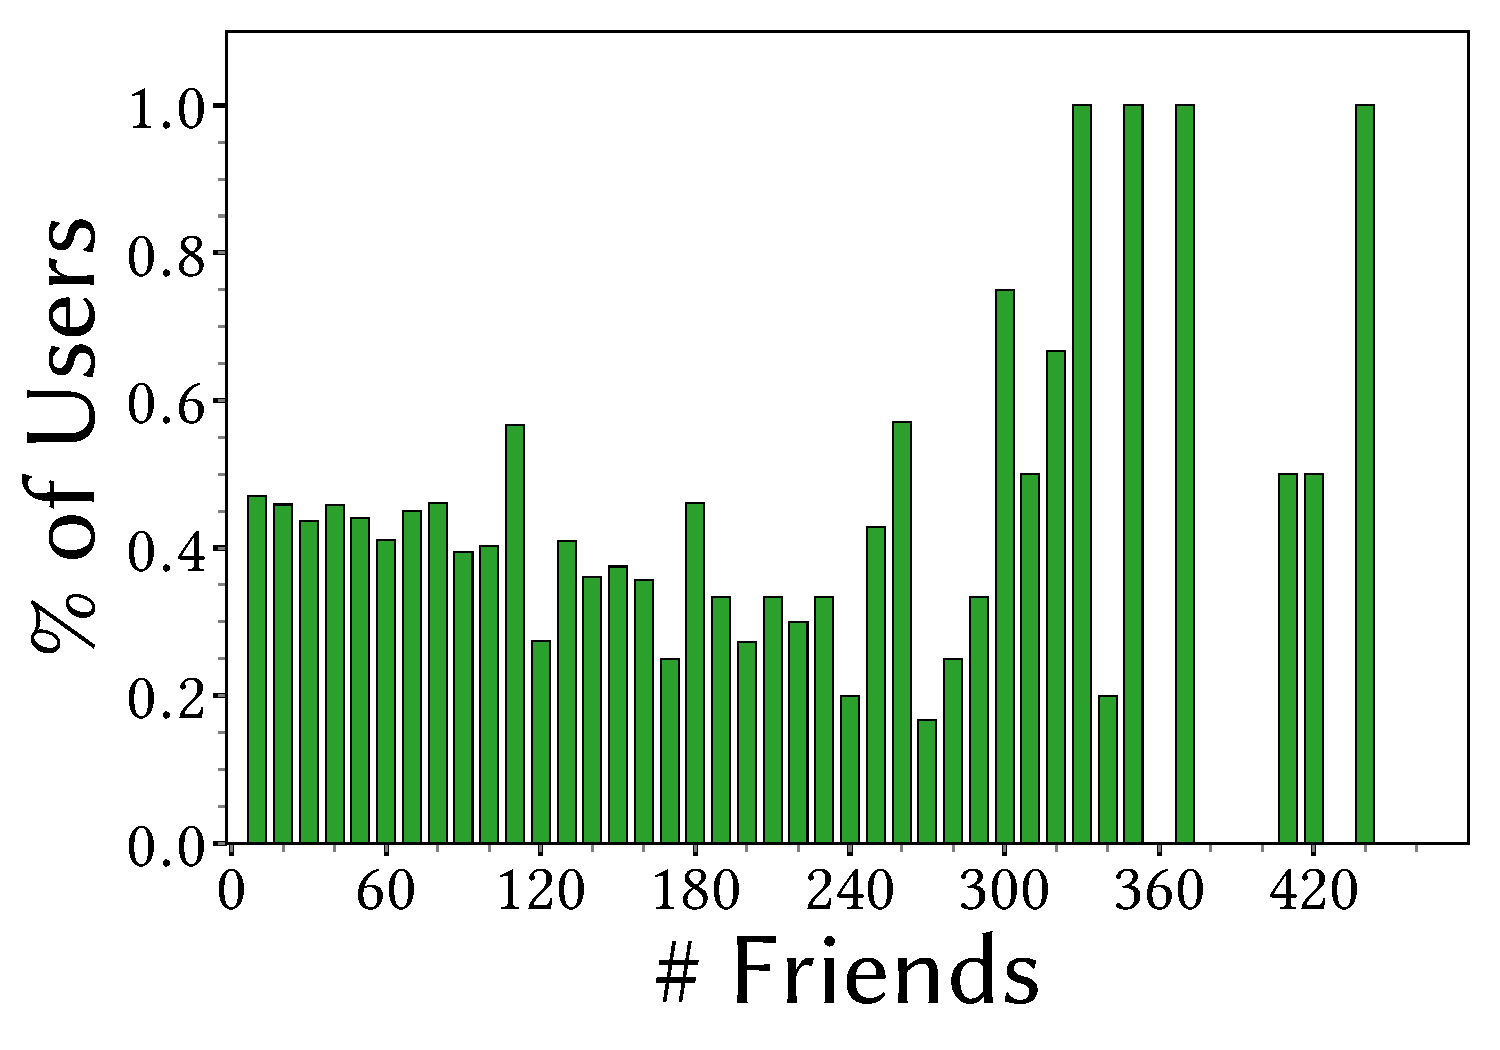
\includegraphics[height=4cm,width=0.3\linewidth]{figures/epinions_itemSocial_Total_users_friend.pdf}
 &
    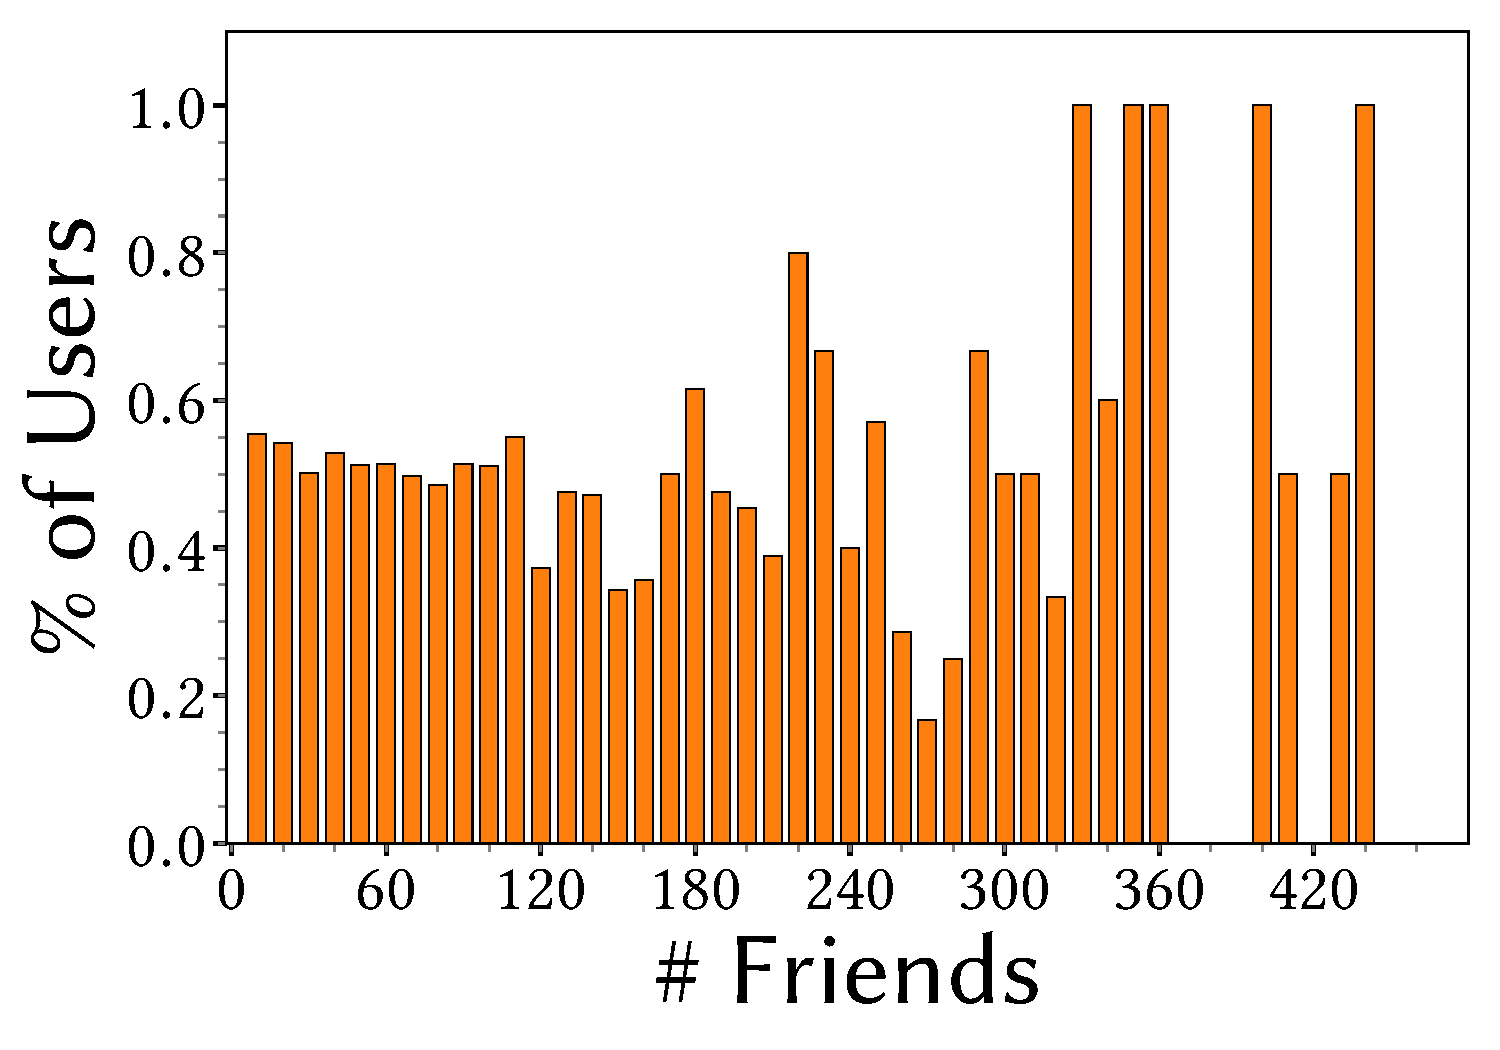
\includegraphics[height=4cm,width=0.3\linewidth]{figures/epinions_userSocial_Total_users_friend.pdf}
  &
    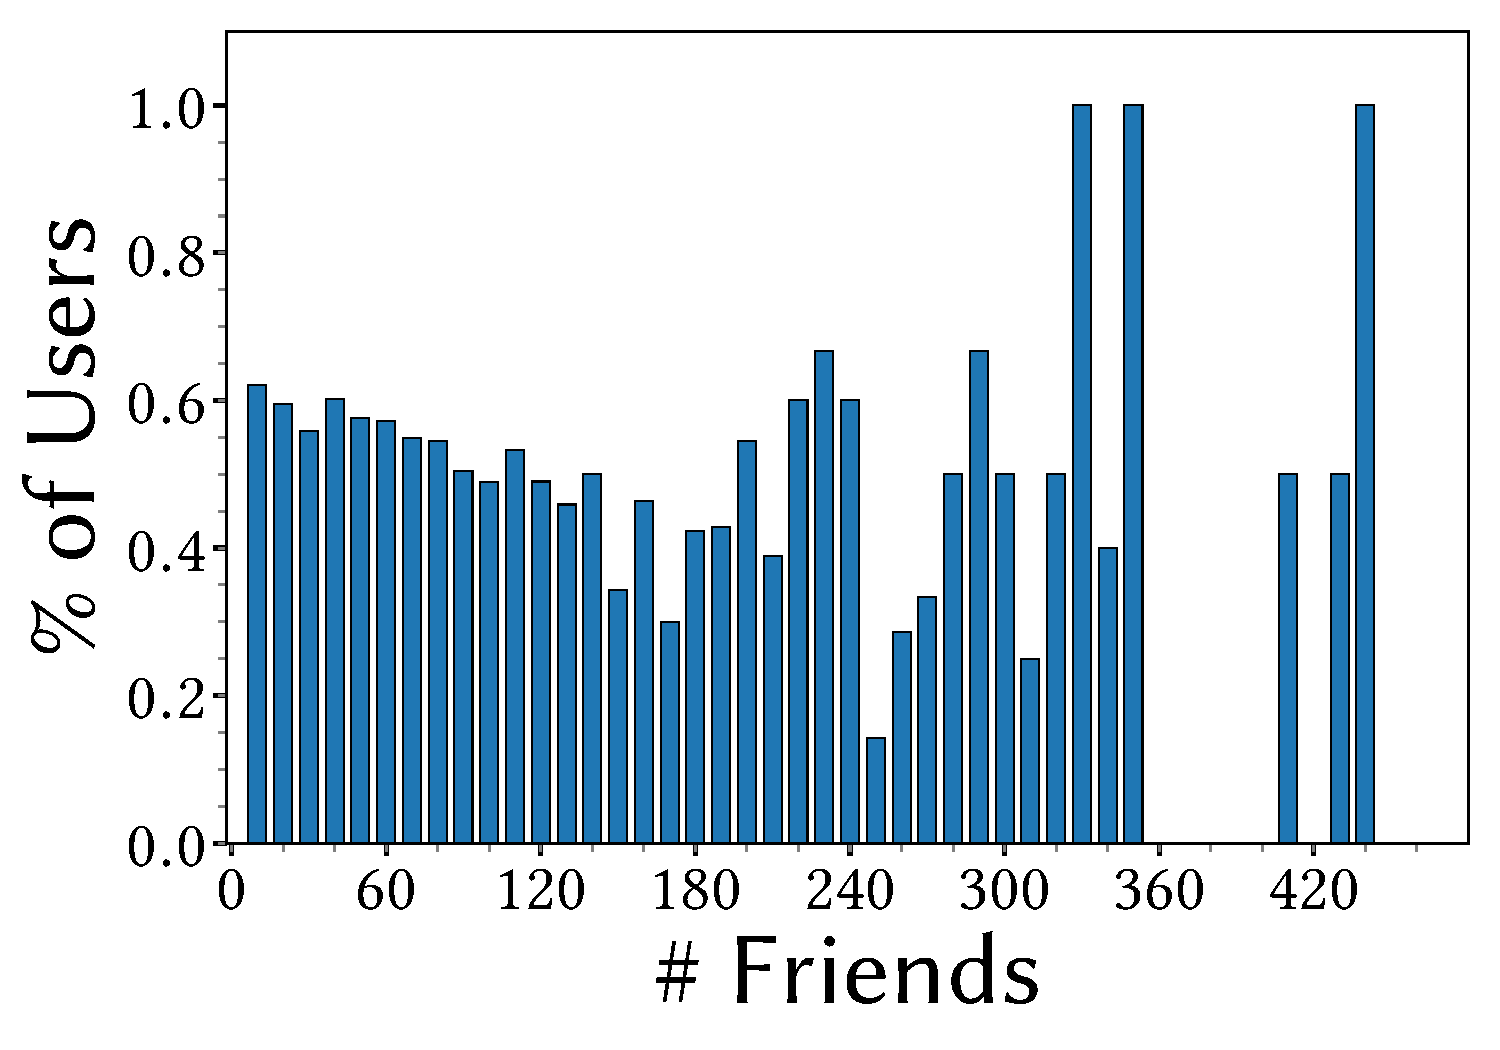
\includegraphics[height=4cm,width=0.3\linewidth]{figures/epinions_temporal_Total_users_friend.pdf}\\
    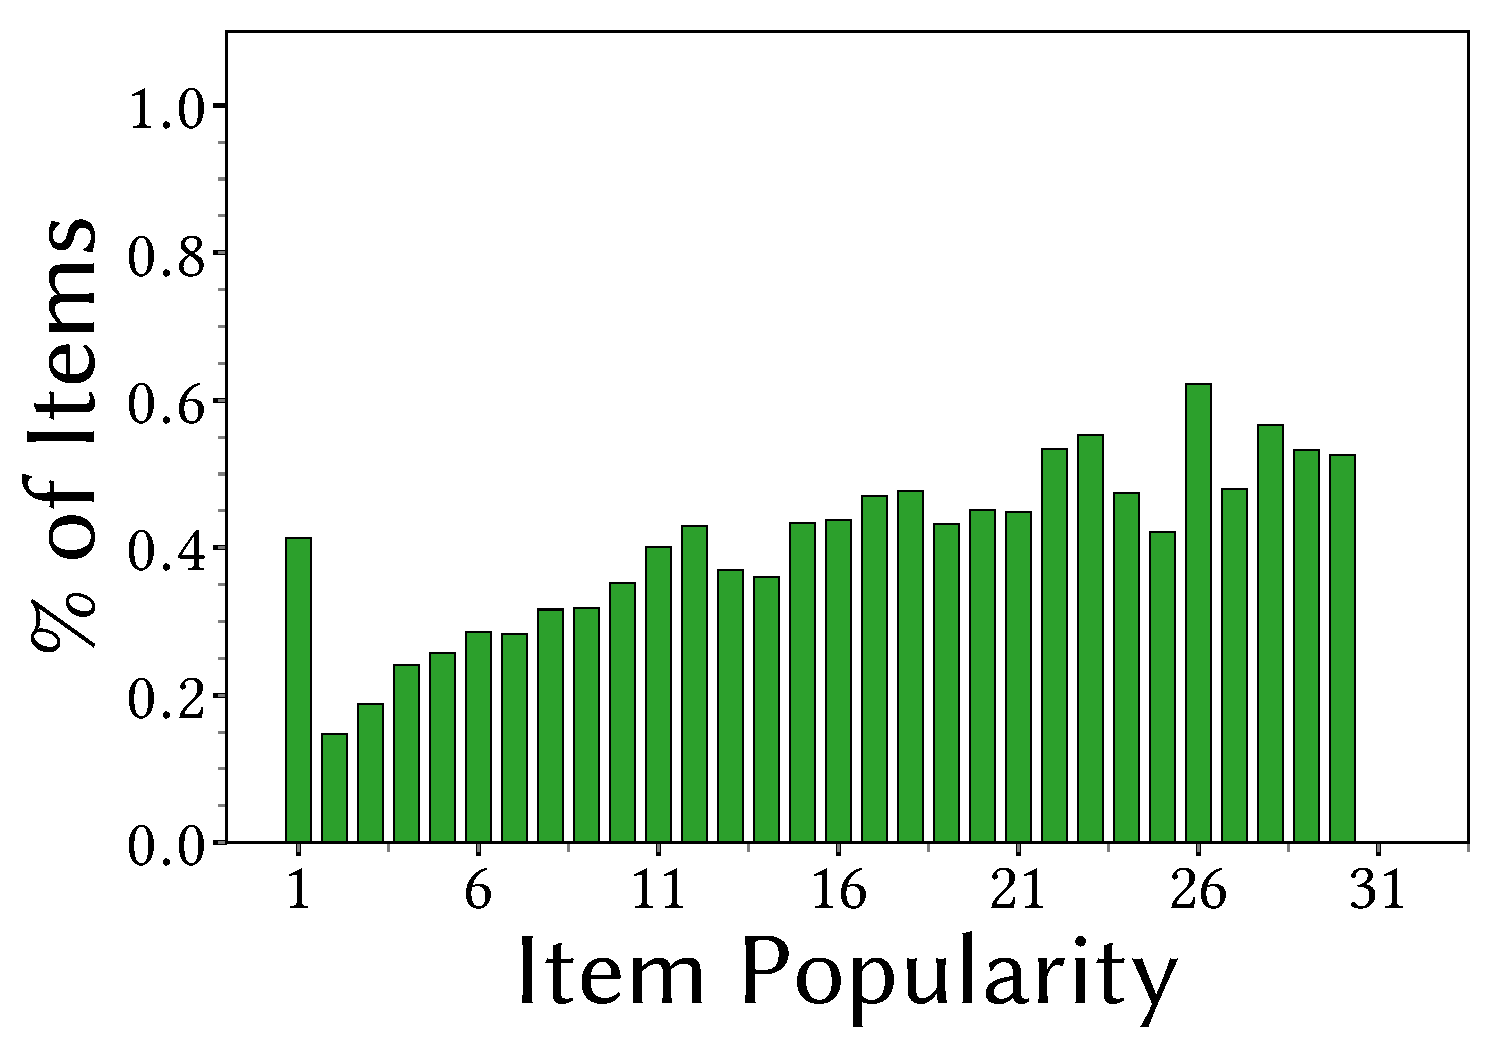
\includegraphics[height=4cm,width=0.3\linewidth]{figures/epinions_itemSocial_Total_items_length.pdf}
 &
    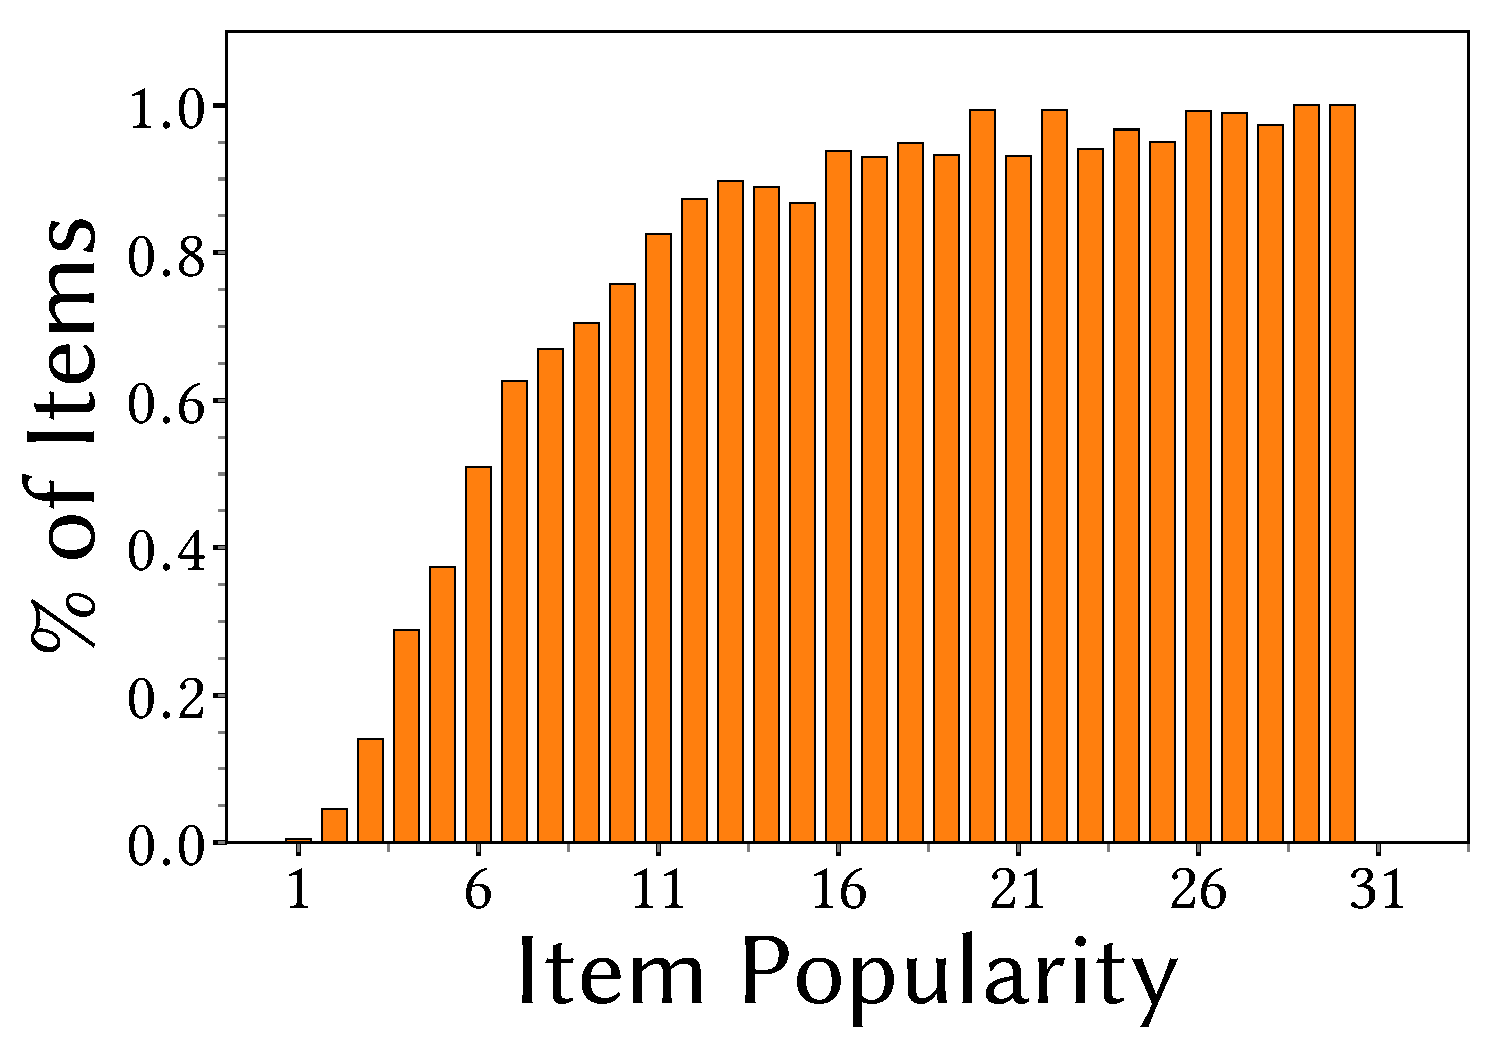
\includegraphics[height=4cm,width=0.3\linewidth]{figures/epinions_userSocial_Total_items_length.pdf}
  &
    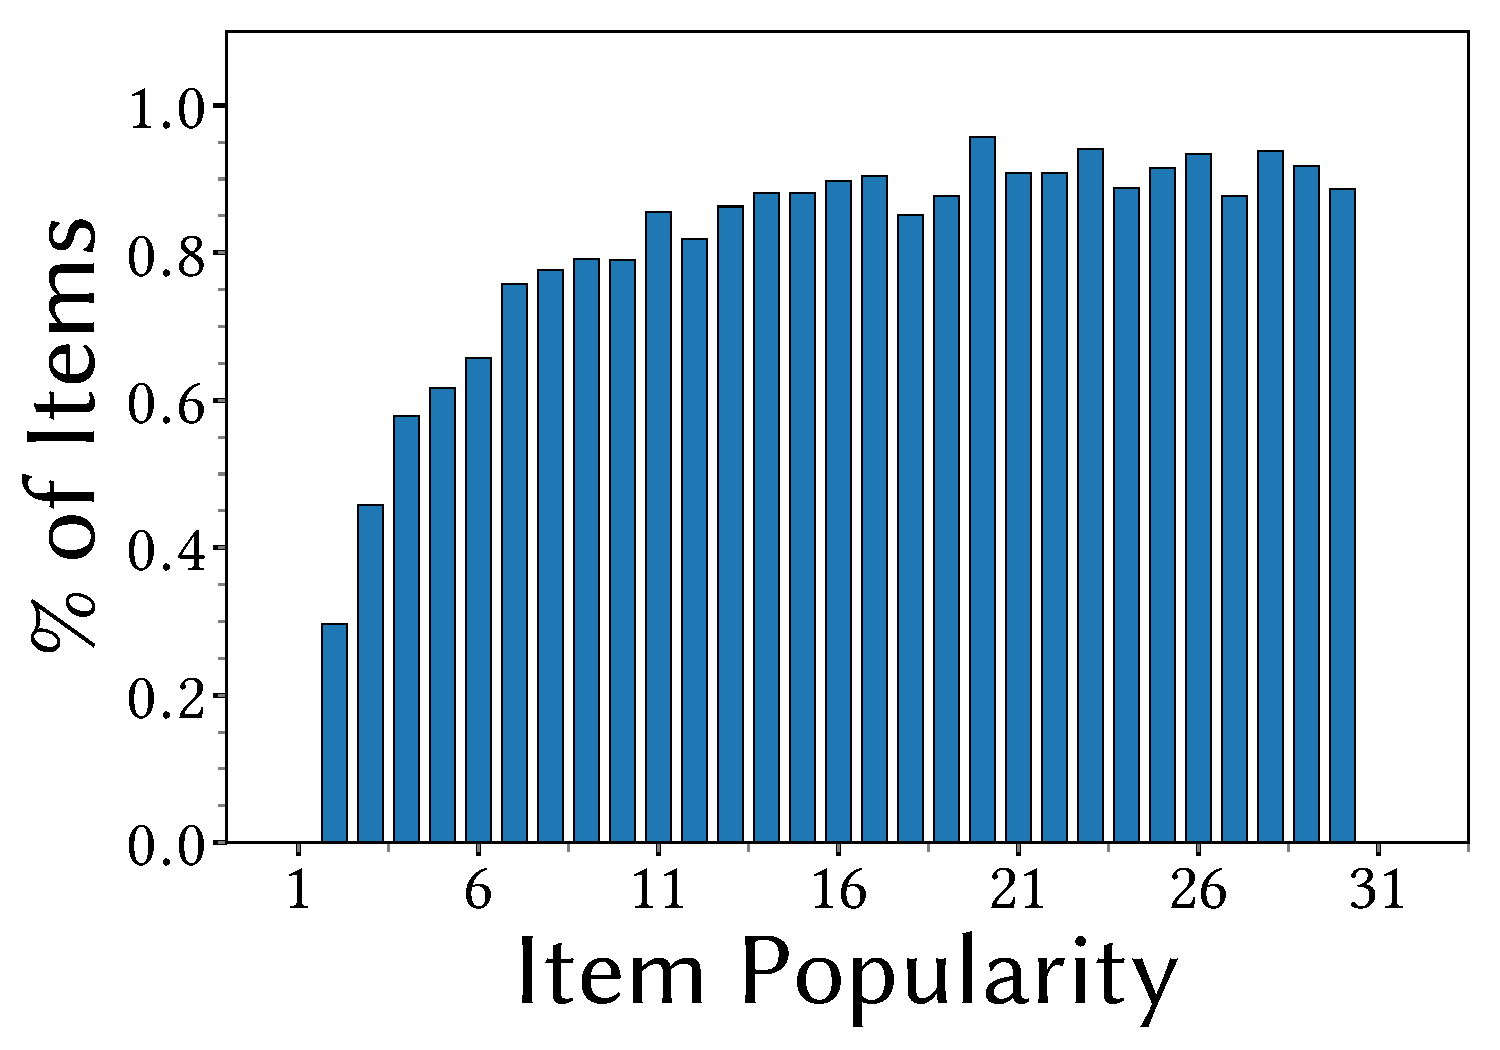
\includegraphics[height=4cm,width=0.3\linewidth]{figures/epinions_temporal_Total_items_length.pdf}\\
  \end{tabular}
  \caption{ Fraction of correct item predictions on test data by %GATRec model and its
  individual modules with different user sequence length, varying size of a user's social connections and varying item popularity. The item-similarity module performs better for rare items while the user-social module better models cold-start users.}
  \label{fig:analysis}
\end{figure}

Further, we evaluated individual modules with varying item popularity in the dataset, different sequence length for users, and varying size of a user's social graph for the Epinions dataset as shown in \Cref{fig:analysis}.
The user-social module is able to predict cold-start users better than the user-temporal module as it takes information from a user's social connections into account (top row). Note, the item-similarity module performs uniformly for different user sequence length as it does not contain any user information. Information about the past behavior of social connections (user-social module) improves performance compared to not using social connections (item-similarity module). Note that this effect increases with more friends and does not create noise as our attention model can distinguish between strong and weak connections (middle row).
The item-similarity module exploits item homophily in the user space and the feature space. Thus, it can accurately predict rarely reviewed items (in the left section of the figure, close to zero) better than the other two modules (bottom row).
Thus, our model provides an interpretable way of determining the importance of each of the factors used in our model through multiple experiments.


\subsection{Cold-Start Analysis} Combining different factors in each of the three modules helps to alleviate data sparsity and to predict for cold-start users effectively. To verify this claim, we evaluate our model in cold-start settings using a decreasing number of past available interactions for a user. \Cref{fig:ablationAUC}
provides our results with varying user sequence length compared to the baselines. Our model significantly outperforms the baselines modeling a subset of the factors for cold-start settings on all the three datasets reaffirming our claim.
Also, we observe that our model performs comparably for user history lengths 10 and above, while the performance drops for very short sequence length of 5. This further underlines that a user's temporal history is an essential cue for the recommendation.

\begin{figure}[tbh]
 \centering
 \begin{subfigure}[b]{\linewidth}
   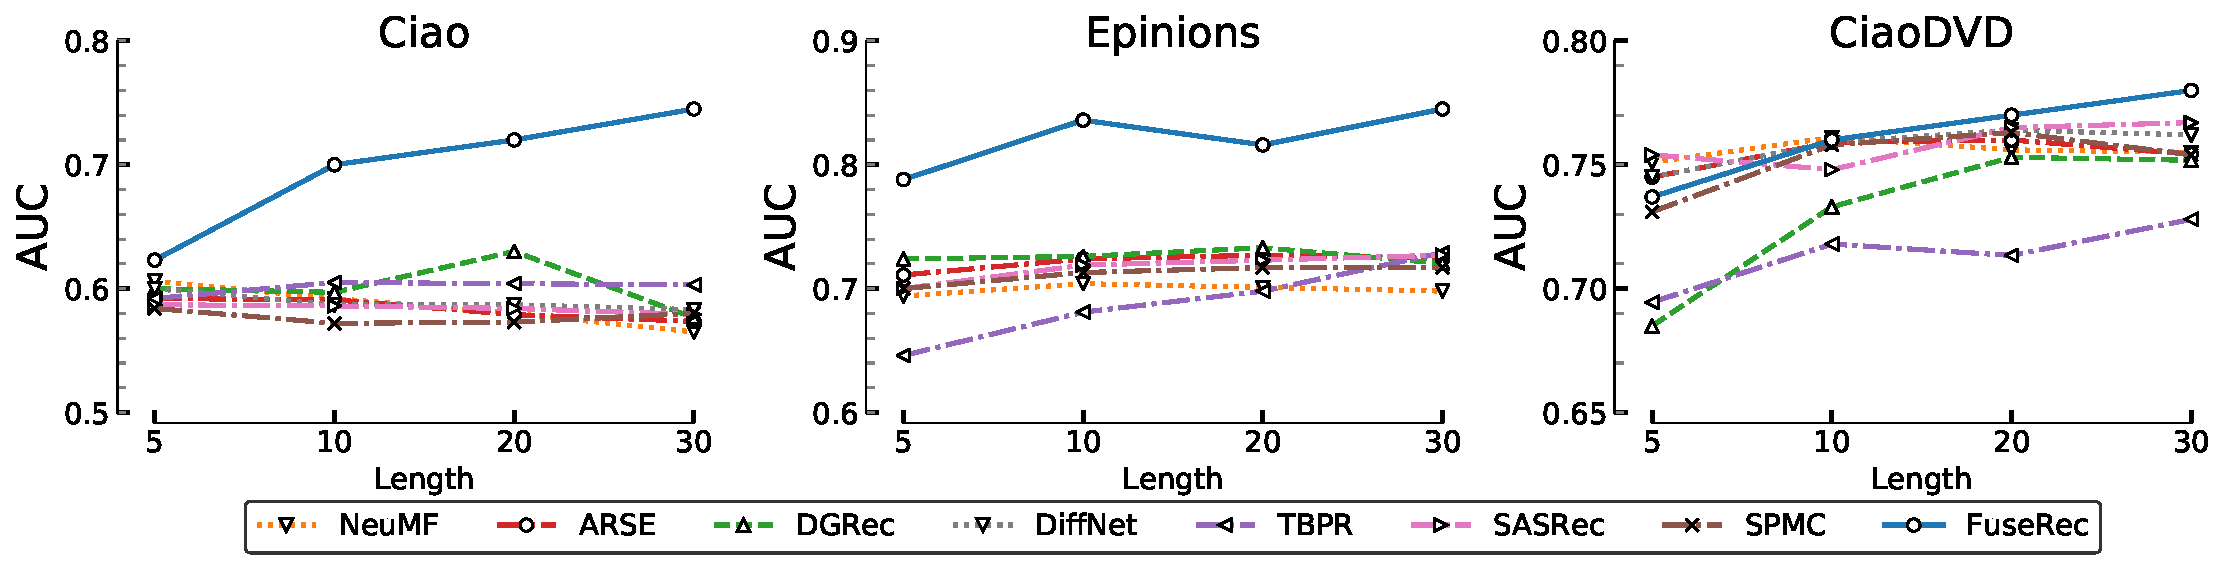
\includegraphics[width=1\linewidth]{figures/AUC.pdf}
 \end{subfigure}
 \caption{\label{fig:ablationAUC}AUC  over different number of  past interactions to mimic cold-start settings. Our model consistently outperforms all the social and temporal based baselines.}
\end{figure}

\subsection{Parameter Sensitivity}

\begin{table}[tbh]
    \centering
    \begin{tabular}{l c c c c c c } \toprule
     & \multicolumn{2}{c}{Ciao} & \multicolumn{2}{c}{Epinions} & \multicolumn{2}{c}{CiaoDVD}\\
     &  HR@10   &    AUC         &    HR@10   & AUC &    HR@10   & AUC \\ \hline
    No Attn & 0.313 & 0.707 & 0.536  & 0.697 & 0.515 & 0.742\\
    User\-side Attn & 0.356  & 0.719 &  0.531 & 0.729 & 0.532 & 0.747\\
    Item\-side Attn & 0.356 & 0.737 & 0.541 & 0.740 & 0.536 & 0.752\\
    \ours & 0.355 & 0.745 & 0.549 & 0.834 & 0.538 & 0.774\\
     \bottomrule
    \end{tabular}
\caption{Performance of our model without attention in the user-social and the item-similarity module. Attention in item-similarity module only performs better than only user-social module attention. }
\label{tab:attention}
\end{table}

\Cref{tab:attention} details performance results after removing attention from our user-social and item-similarity modules, respectively. The variant without attention on both the modules performs the worst. Comparing the user-social and item-similarity module: only using attention in the item-similarity module performs better than using attention in the user-social module exclusively. This is expected as the ties between similar items are weaker than explicit social connections between users. Thus, attention results in lower weights for noisy connections in the item-similarity module.

\begin{figure}[tbh]
 \centering
   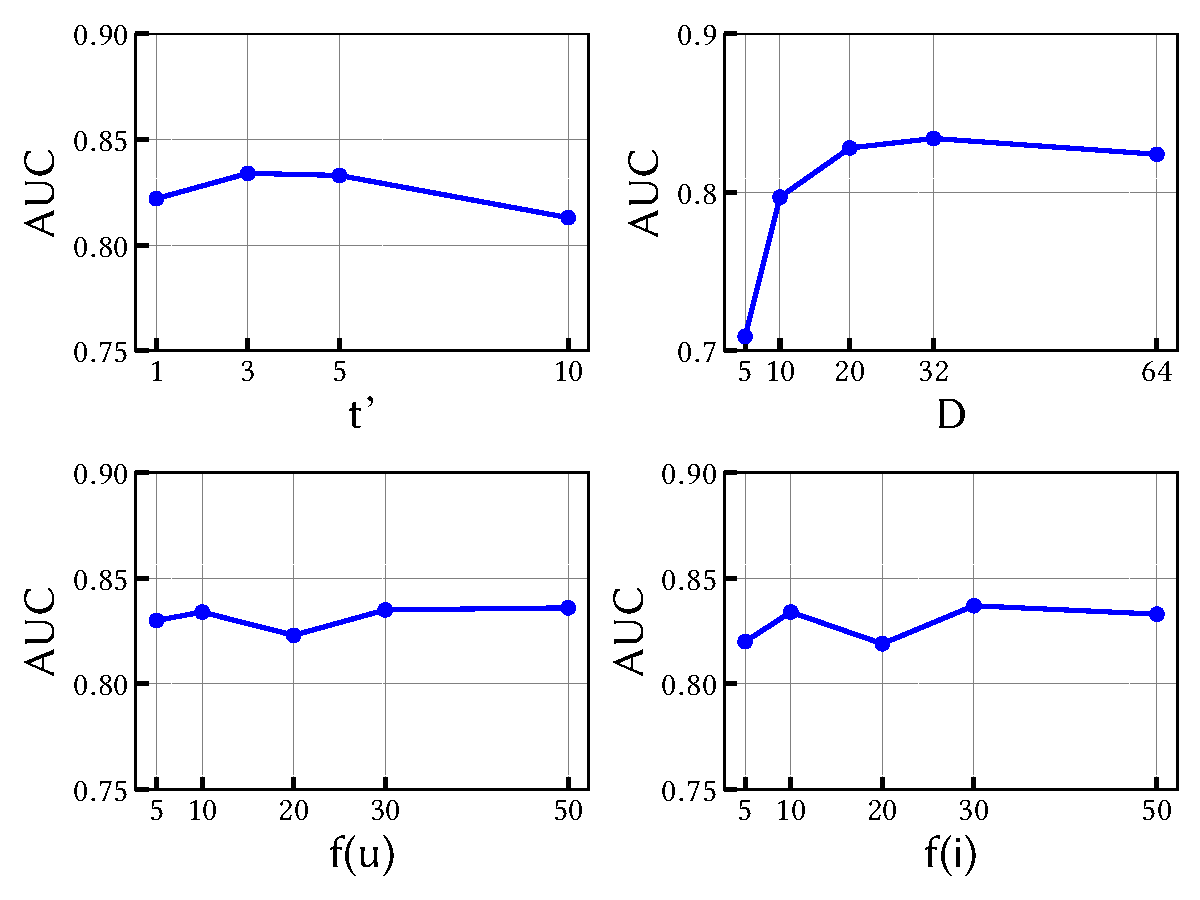
\includegraphics[scale=0.5]{figures/Ablation_new.pdf}
 \caption{Ablation results of different model hyper-parameters on Epinions datatset.}
 \label{fig:ablation}
\end{figure}

\Cref{fig:ablation} illustrates the performance of our model with different hyper-parameters on the Epinions dataset. For a user's friend's history length $t'$ (\Cref{eq:useragg}),  we observe: using fewer past interactions performs better. However, no change in performance is observed if $t'$ increases to more than the last five interacted items.
Increasing the size of the hidden dimension $D$ improves performance initially due to larger model capacity. However, results decline beyond a certain point due to overfitting.
For the user and item friend sample size, $F(u)$ (\Cref{eq:user}) and $F(i), F'(i)$  (\Cref{eq:item}) respectively, performance slightly increases with an increased size but plateaus for  sample sizes larger than 10.

\subsection{Induced relationships}

We further experimented with different graphs both in the User-Social and Item-Similarity module. In the user-social module, apart from the explicit social connections, we also induced another user graph based on similar preferences. Specifically, we computed k-nearest neighbors for each user using cosine similarity between their past item interactions. Similar to item graphs, we keep $k = 30$ for the user induced graph.
While for the item side, we experiment with two different graphs, one based on feature similarity between items, and another is based on frequent co-occurrence in the user's history.

Table \ref{tab:graph} details performance results when using different user and item graphs for all datasets. In general, using an induced user graph based on similar history performs competitively or slightly outperforms the explicit social graph. This reaffirms our hypothesis that connected users exhibit similar behavior. Note that computing similar users can be computationally expensive if the dataset is large.

\begin{table}[h]
    \centering
    \begin{tabular}{l l c c c c c c } \toprule
     & & \multicolumn{2}{c}{Ciao} & \multicolumn{2}{c}{Epinions} & \multicolumn{2}{c}{CiaoDVD}\\
     User Graph & Item Graph &  HR@10   &    AUC         &    HR@10   & AUC &    HR@10   & AUC \\ \hline
    Social & Co-Occurrence & 0.308 & 0.743 & 0.518  & 0.805 & 0.554 & 0.749\\
    Social & Feature & 0.292 & 0.709 & 0.520  & 0.827 & 0.537 & 0.747\\
    Induced & Both & 0.320 & 0.753 & --  & -- & 0.540 & 0.763\\
    Social & Both & 0.355 & 0.745 & 0.549 & 0.834 & 0.538 & 0.774\\
     \bottomrule
    \end{tabular}
\caption{Performance of our model with different graphs in the user-social and the item-similarity module. Induced relationships in the user graph fare little better than explicit social connections. In the item space also, item graph based on frequent co-occurrence in the user history is a better indicator of future item prediction. We could not extract induced user graph in Epinions because of out of memory error.}
\label{tab:graph}
\end{table}

In the item space, for Ciao and CiaoDVD, the co-occurrence graph performs better than the feature similarity graph. This competent performance is intuitive as most of the item collaborative filtering methods also leverage co-occurrence for providing recommendations. Besides, a similar item category may not be a strong signal of repeat user behavior as users tend to buy things across different categories.

% !TEX root = SADR.tex
\section{Conclusion}
We presented a model which captures temporal changes and socio-temporal influence while taking into account item similarity and later combines them in an interpretable manner.
We used an RNN model to capture the evolution of user preferences. We proposed an attention based user social module which aggregates historical features for all of the user's neighbors. To capture item-based homophily, we proposed an attention based item module to learn item embeddings using similar items frequently co-occurring in the platform.
We compared our approach to a large number of temporal, social, and socio-temporal recommenders on three benchmark datasets. We report an improvement of more than 13\%
over state-of-the-art baselines on the  Ciao and Epinions datasets for AUC metric.
Our ablation study shows that each module is essential to capture different factors affecting user behavior in recommender systems. Further, user-temporal module is most important factor across all datasets.


\chapter{Modeling relational aspects of user-generated content}
\label{chap:induced}
In this chapter, we propose to incorporate user behavioral information as metadata to improve the attribute estimation of user-generated content.
For this purpose, we focus on the task of quality estimation of user-provided answers for best answer selection task in CQA forums. Current approaches predict answer quality in isolation of the other answers to the question and user activity across the forum (other posted questions or answers). This assumption is limiting as the best answer is, in general, selected based on how it differs from other answers to the same question. Similarly, answers given by expert users tend to be of higher quality. We leverage these cues by inducing multiple graphs between these answers based on similarity and contrast in the behavior of users providing the answers. Finally, multiple graphs expressing semantically diverse relationships
are merged to predict the best answer to a question \cite{induced}.

\section{Overview}
Individuals often visit Community Question Answer (CQA) forums, like StackExchange, to seek answers to nuanced questions that are not readily available on web-search engines.
Unlike other familiar Learning-to-Rank problems in the IR community~\cite{LambdaMart, LambdaNet}, CQA platforms can identify and leverage past questions asked by similar users and relevant answers to those questions.
However, for CQA sites like StackExchange, individuals who post questions may label an answer as `accepted,' but other questions with answers (about $47$\% in our analysis) have none labeled as `accepted.' On other CQA sites like Reddit, there is no mechanism for a person to label an answer as `accepted.' As a first step to address the individual's information needs, in this work, we focus on the problem of identifying accepted answers on StackExchange.

One approach to identify relevant answers is to identify salient features for each question-answer tuple $(q,a)$ and treat it as a supervised classification problem~\citep{BurelMA16,  JendersKN16, TianZL13, TianL16}. Deep Text Models further develop this approach~\cite{ZhangLSW17, WuWS18, WangN15, SukhbaatarSWF15}. These models learn the optimal text representation of $(q,a)$ tuple to select the most relevant answer. While the deep text models are sophisticated, text-based models are computationally expensive to train. Furthermore, there are limitations to examining $(q,a)$ tuples in isolation: an answer is "relevant" \emph{in relationship} to other answers to the same question; second, it ignores the fact that same user may answer multiple questions in the forum.
These relational aspects of user-generated content provide a unique dimension that is absent in textual search. However, there is only limited work in the context of identification of "best answers" among user-generated content that exploit these implicit and explicit connections.
Thus, our key proposal is to use this alternative approach and build a flexible and expressive framework to incorporate the relational aspects of user-generated content for the answer selection task.

Relational aspects are best captured as graphs connecting content.
Graph Convolutional Networks (GCNs) is a popular technique to incorporate graph structure, and are used in tasks including node classification \cite{gcn} and link prediction~\cite{relationalGCN}. Extensions to the basic GCN model include signed networks~\cite{signedgcn}, inductive settings~\cite{graphsage} and multiple relations~\cite{DualGCN, relationalGCN}.
While GCNs are a plausible approach, we need to overcome a fundamental implicit assumption in prior work before we can apply it to our problem. Prior work in GCNs adopt label sharing amongst nodes; label sharing implicitly assumes similarity between two nodes connected by an edge. In the Answer Selection problem, however, answers to the same question connected by an edge may not share the acceptance label. In particular, we may label an answer as `accepted' based on how it differs from other answers to the same question.
In other words, the relational views (or graphs) could capture similarity or contrast between connected content, depending on the relation in consideration.
However, Signed GCNs~\cite{signedgcn} can not capture this contrast despite their ability to incorporate signed edges. Graph attention networks~\cite{graphattention} also could not learn negative attention weight over neighbors as weights are the output of a softmax operation.

Thus, we develop a novel framework to model the diverse relations between content through a separate \textit{induced} graph across $(q,a)$ tuples. The key idea is to use diverse strategies---label depends only on the answer (reflexive), the label is determined in contrast with the other answers to the question (contrastive), and label sharing among answers across questions if it contrasts with other answers similarly(similar contrast)---to identify the accepted answer.
Each strategy \textit{induces} a graph between $(q,a)$ tuples and then uses a particular label selection mechanism to identify the accepted answer. Our strategies generalize to a broader principle: pick an equivalence relation to induce a graph comprising cliques, and then pick a label selection mechanism (label sharing or label contrast) within each clique. We show how to develop GCN architecture to operationalize the specific label selection mechanism (label sharing or label contrast). Then, we aggregate results across strategies through a boosting framework to identify the label for each $(q,a)$ tuple. Our Contributions are as follows:
\begin{description}
  \item[Modular, Induced Relational Framework:] We introduce a modular framework that separates the construction of the graph with the label selection mechanism. In contrast,  prior work in answer selection (e.g.,~\citep{BurelMA16,  JendersKN16, TianZL13, TianL16}.) looked at individual tuples, and work on GCNs (e.g.,~\citep{gcn, DualGCN}) use the given graph (i.e., no induced graphs) and with similarity as a mechanism for label propagation. We use equivalence relations to induce a graph comprising cliques and identify two label assignment mechanisms---label contrast, label sharing. Then, we show how to encode these assignment mechanisms in GCNs. In particular, we show that the use of equivalence relations allows us to perform \textit{exact} convolution in GCNs. We call our framework Induced Relational GCN (IR-GCN). Our framework allows for parallelization and applies to other problems that need application semantics to induce graphs independent of any existing graphs\cite{InducedGraph}.
  \item[Discriminative Semantics:] We show how to encode the notion of label contrast between a vertex and a group of vertices in GCNs. Label contrast is critical to the problem of best answer selection. Related work in GCNs (e.g.,~\citep{gcn, DualGCN}) emphasizes node similarity, including the work on signed graphs~\cite{signedgcn}. In~\citep{signedgcn}, contrast is a property of an edge, not a group, and is not expressive enough for our problem. We show that our encoding of contrast creates \textit{discriminative magnification}---the separation between nodes in the embedding space is most meaningful at smaller clique sizes; the effect decreases with clique size.

  \item[Boosted Architecture:]  We show through extensive empirical results that using common boosting techniques improves learning in our convolutional model. This improvement is a surprising result since much of the work on neural architectures develops stacking, fusion, or aggregator architectures.

\end{description}

We conducted extensive experiments using our IR-GCN framework with excellent experimental results on the popular CQA forum---StackExchange. For our analysis, we collect data from 50 communities---the ten largest communities from each of the five StackExchange\footnote{https://stackexchange.com/sites} categories. We achieved an improvement of over 4\% accuracy and 2.5\% in MRR, on average, over state-of-the-art baselines. We also provide Reddit \footnote{https://www.reddit.com/} results using expert answers as a proxy for acceptance, to overcome the absence of explicit labels. Finally, we show that our model is more robust to label sparsity compared to alternate GCN based multi-relational approaches.

We organize the rest of this chapter as follows. In \cref{sec:problem}, we formulate our problem statement and then discuss induced relations for the Answer Selection problem in \cref{sec:Induced Relational Views}. We then detail the operationalization of these induced relations in the Graph Convolution framework in \cref{sec:gcn} and introduce our gradient boosting based aggregator approach in \cref{sec:aggregation}. \Cref{sec:induced_experiments} describes experiments and \Cref{sec:discussion} describes further ablation studies. We finally conclude in \cref{sec:conclude}.

\section{Problem Formulation}
\label{sec:problem}
In Community Question Answer (CQA) forums, an individual asking a question seeks to identify the most relevant candidate answer to his question. On Stack-Exchange CQA forums, users annotate their preferred answer as ``accepted.''

Let $\mathcal{Q}$ denote the set of questions in the community and for each $q \in \mathcal{Q}$, we denote $\mathcal{A}_q$ to be the associated set of answers. Each question $q \in \mathcal{Q}$, and each answer $a \in \mathcal{A}_q$ has an author $u_q, u_a \in \mathcal{U}$ respectively. Without loss of generality, assume that we can extract features for each question $q$, each answer $a \in \mathcal{A}_q$, user $u_q, u_a \in \mathcal{U}$.

Our unit of analysis is a question-answer tuple $(q,a), q \in \mathcal{Q}, a \in \mathcal{A}_q$, and we associate each $(q,a)$ tuple with a label $y_{q,a} \in \{-1,+1\}$, where `+1' implies acceptance and `-1' implies rejection.

\begin{quote}
    The goal of this paper is to develop a framework to identify the accepted answer to a question posted on a CQA forum.
\end{quote}

\section{Induced Relational Views}
\label{sec:Induced Relational Views}
In this section, we discuss the idea of induced relational views, central to our induced relational GCN framework developed in~\Cref{sec:gcn}.
First, in~\Cref{sub:Induced Views}, we introduce potential strategies for selecting the accepted answer given a question. We show how each strategy induces a graph $G$ on the question-answer $(q,a)$ tuples. Next, in~\Cref{sub:Generalized Views}, we show how each of these example strategies is an instance of an equivalence relation; our framework generalizes to incorporate any such relation.

\begin{figure}[h]
    \centering
    \begin{subfigure}{0.25\textwidth}
        \centering
        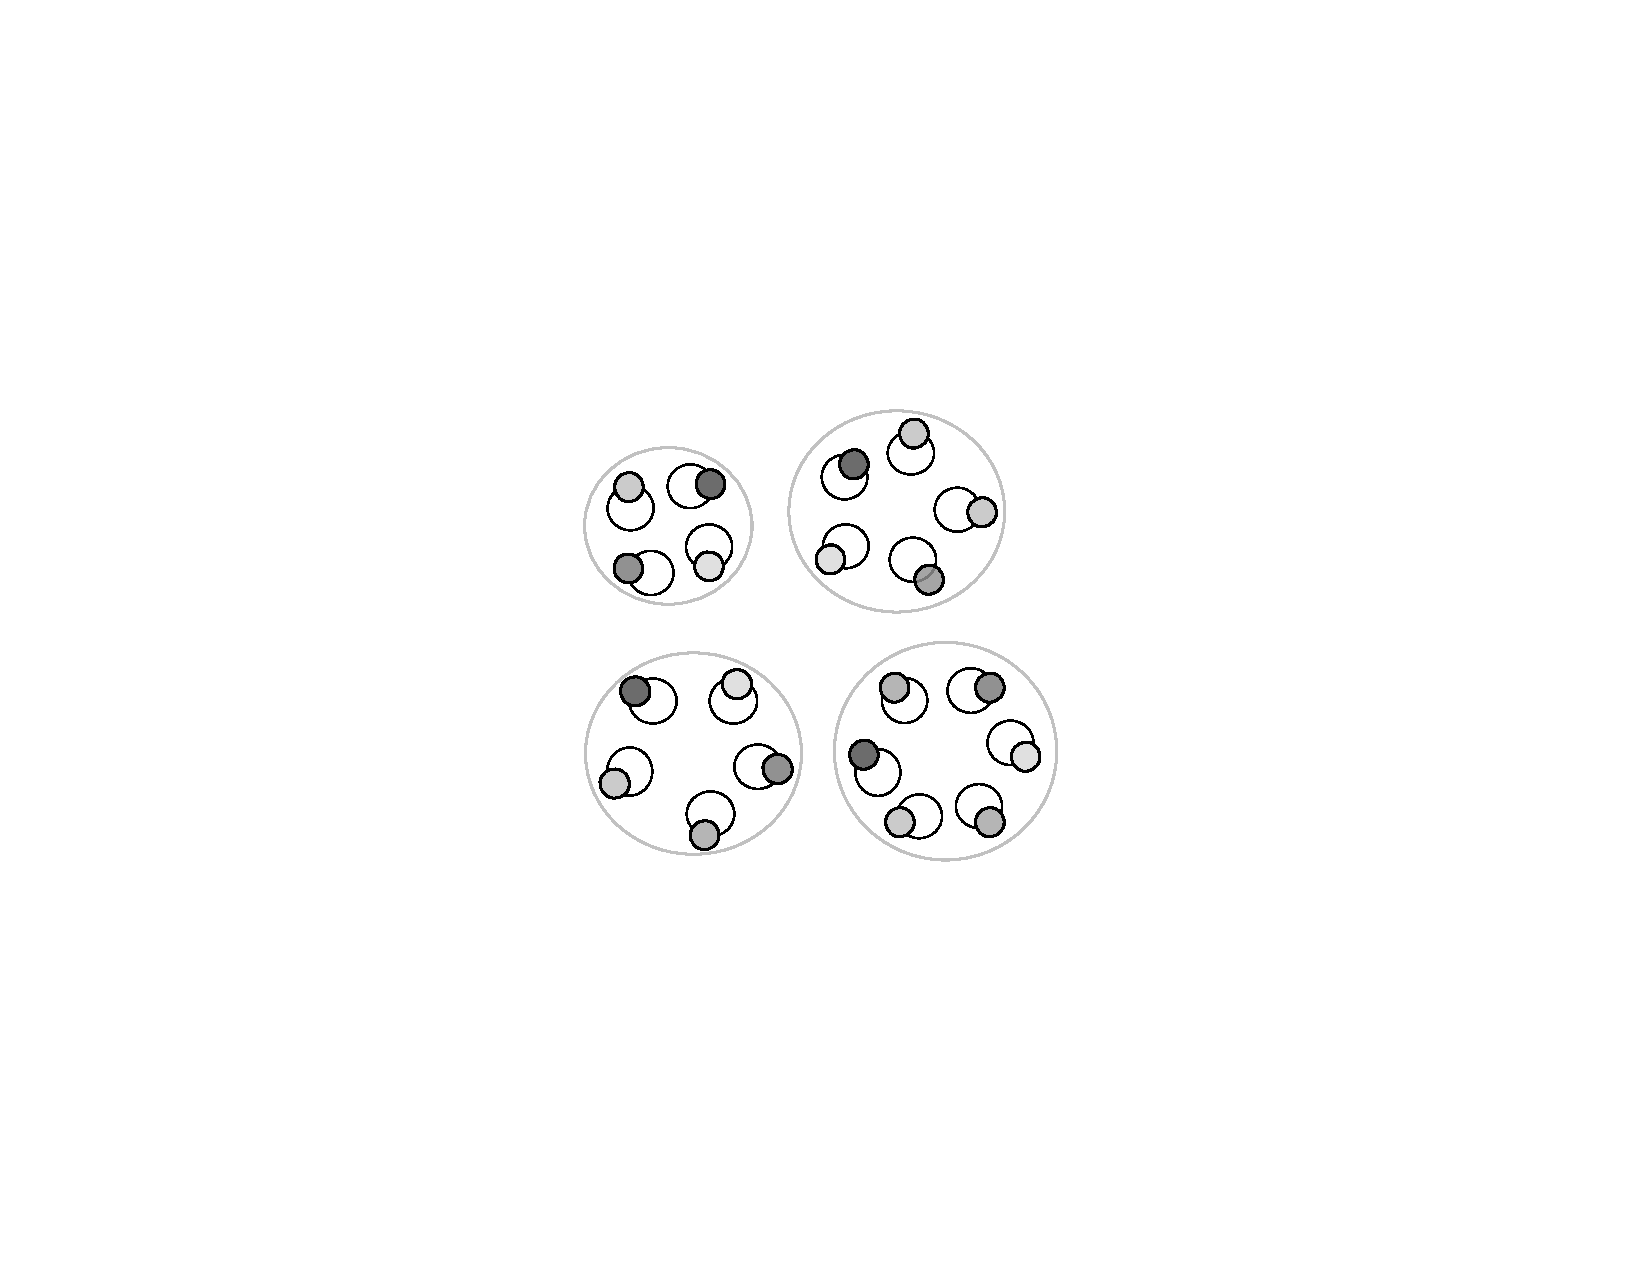
\includegraphics[scale=0.4]{figures/reflex_updated}
            \caption{Reflexive}
            \label{fig:reflexive}
    \end{subfigure}%
    \begin{subfigure}{0.27\textwidth}
        \centering
        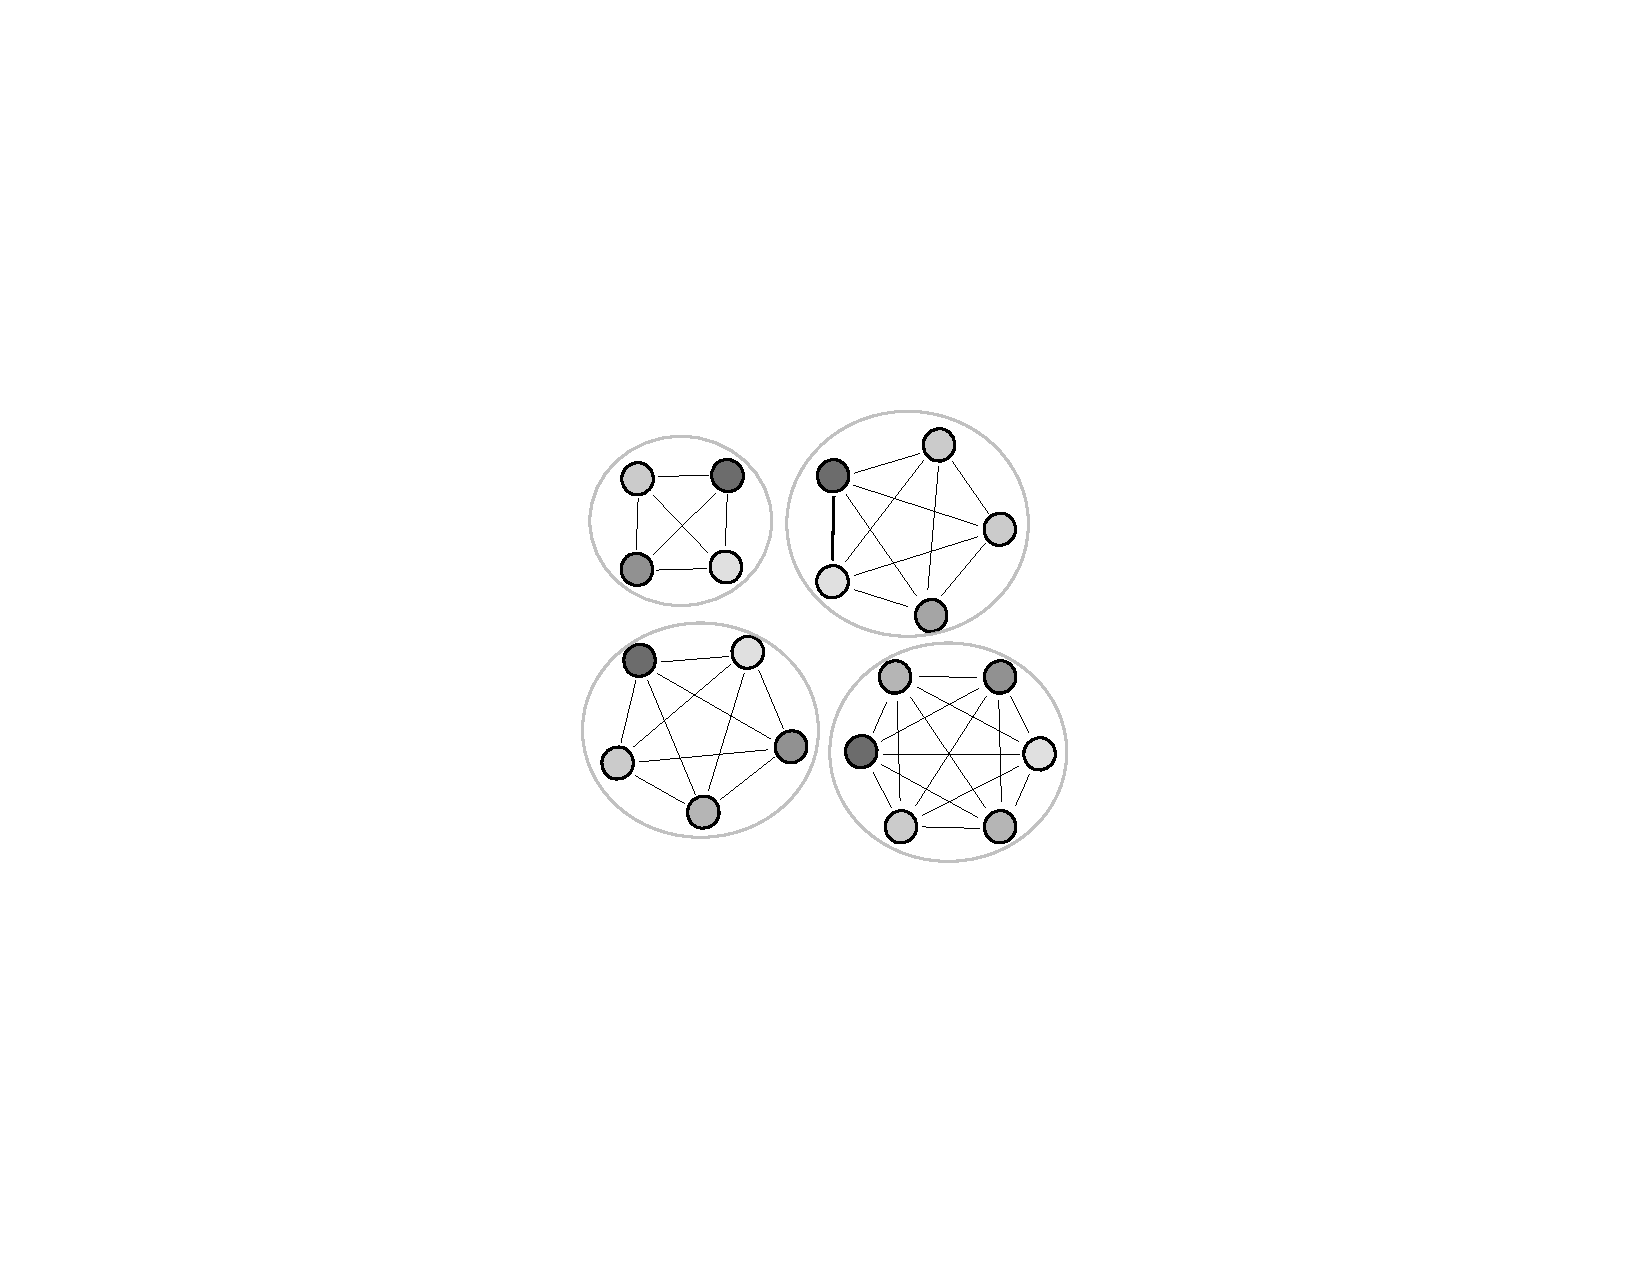
\includegraphics[scale=0.4]{figures/Contrast_circle}
        \caption{Contrastive}
        \label{fig:contrastive}
    \end{subfigure}%
    \begin{subfigure}{0.25\textwidth}
        \centering
        %\includegraphics[width=\linewidth,height=5cm]{figures/drawing}
            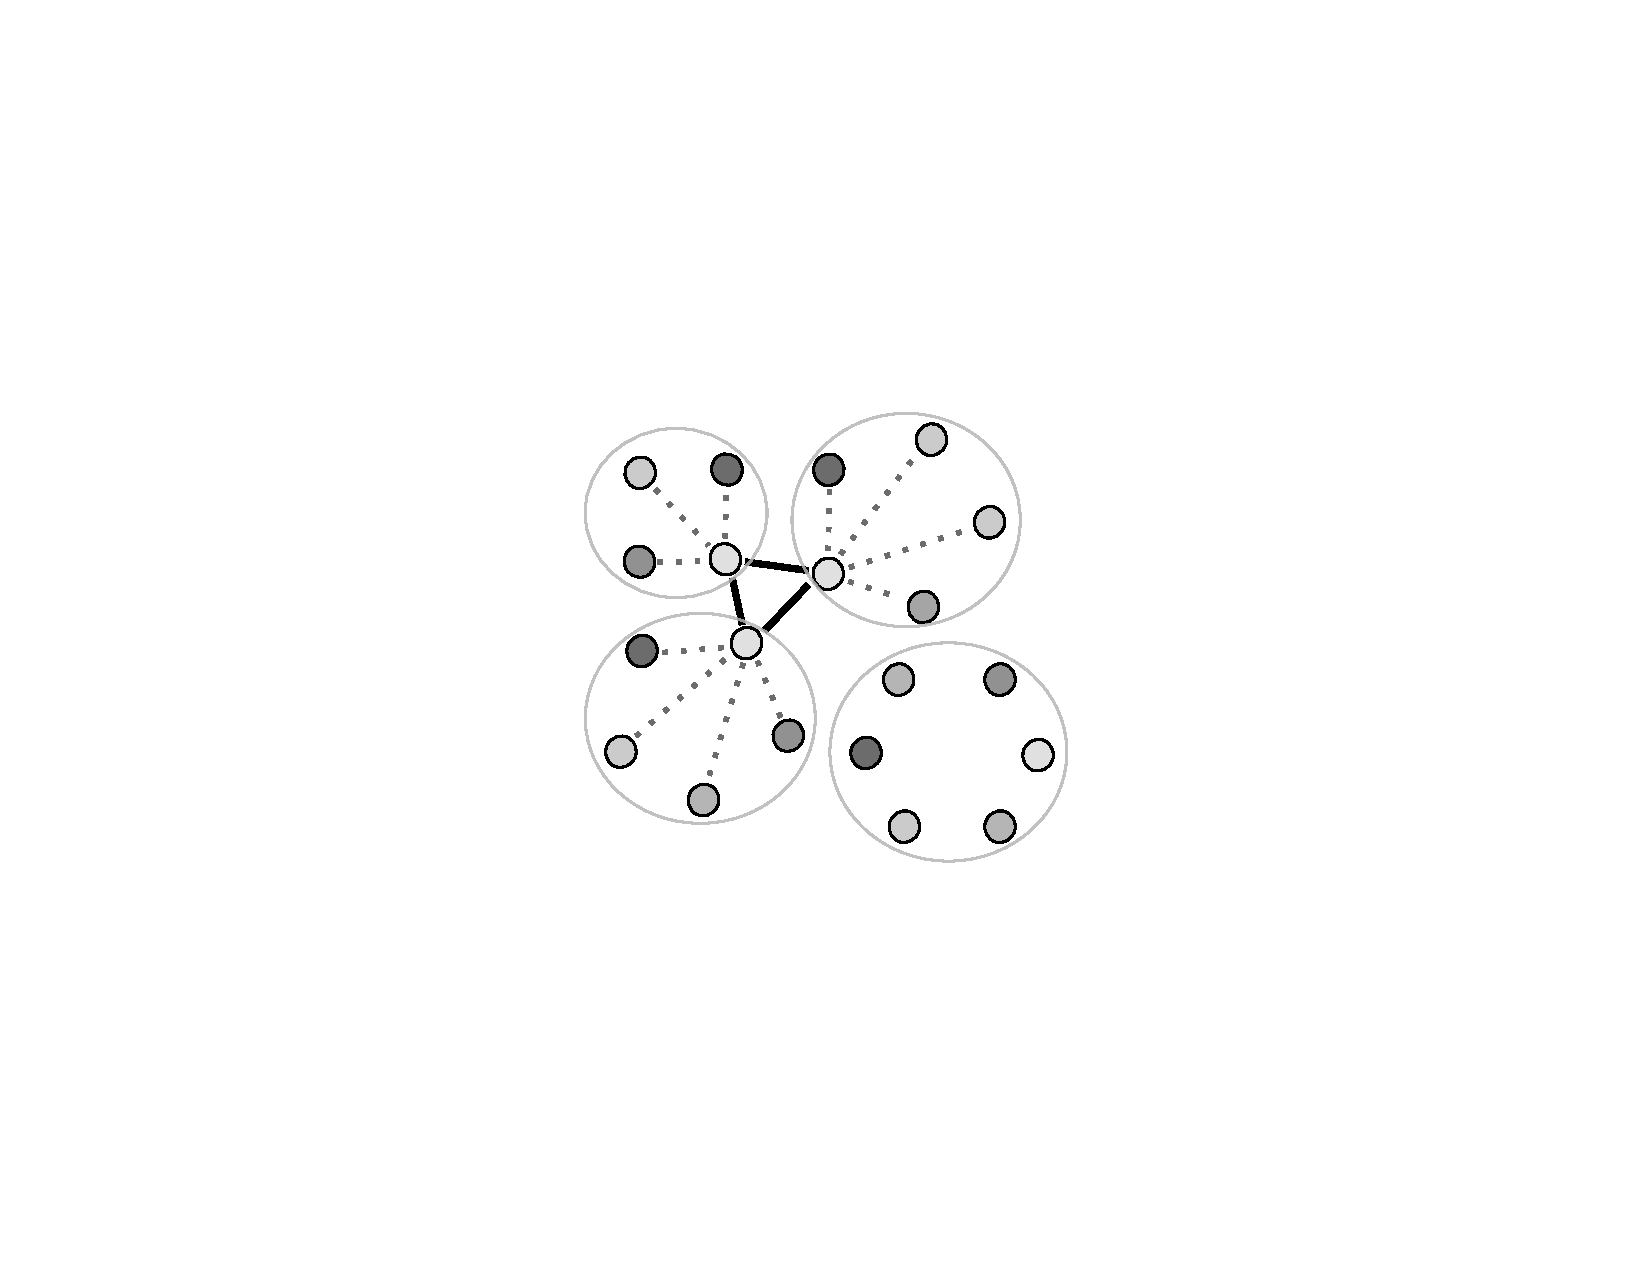
\includegraphics[scale=0.4]{figures/similarContrast_old}
      \caption{Similar Contrast}
      \label{fig:similar}
        \end{subfigure}%
    \caption{\label{fig:relation} Reflexive(~\cref{fig:reflexive}), Contrastive (~\cref{fig:contrastive}) and Similar Contrast (~\cref{fig:similar}) relations among $(q,a)$ tuples. Reflexive assumes no dependence on other answers for prediction. Contrastive compares between all answers to a question;  Similar Contrast connects answers across questions if they contrasts with other answers similarly. Solid lines show the similarity relation while dotted lines signify the contrast. The contrast is only significant in three questions.}
\end{figure}

\subsection{Constructing Induced Views}
\label{sub:Induced Views}


In this section, we discuss in detail four example strategies that can be used by the individual posting the question to label an answer as `accepted.'
Each of the $S_i \in \mathbf{S}$ strategies \textit{induces} a graph $G_i = (V, E_i)$ (also referred to as a relational view).
In each graph $G_i$, a vertex $v \in V$ corresponds to a tuple $(q,a)$ and an edge $e \in E_i, E_i \subseteq V \times V$ connects two tuples that are matched under that strategy.
Note that each $G_i$ has the same vertex set $V$, and the edge sets $E_i$ are strategy dependent. Each strategy employs one of the three different relation types---reflexive, contrastive, and similar---to connect the tuples. We use one reflexive strategy, one contrastive, and two similar strategies.
~\Cref{fig:relation} summarizes the three relations. Below, we organize the discussion by relation type.

\textbf{Reflexive:}
\label{sub:Reflexive}
A natural strategy is to examine each $(q,a)$ tuple in isolation and then assign a label $y_{q,a} \in \{-1,+1 \}$ corresponding to `not accepted' or `accepted.' In this case, $y_{q,a}$ depends on only the features of $(q,a)$. This is a \emph{Reflexive} relation, and the corresponding graph $G_r = (V,E_r)$ has a specific structure. In particular, in this graph $G_r$, we have only self-loops, and all edges $e \in E_r$ are of the type $(v,v)$. That is, for each vertex $v \in V$, there are no edges $(v,u)$ to any other vertices $u\neq v \in V$. Much of the prior work on feature driven answer selection~\cite{BurelMA16,  JendersKN16, TianZL13, TianL16} adopts this view.

\textbf{Contrastive:}
\label{sub:Contrastive}
A second strategy is to examine answers \textit{in relation} to other answers to the same question and label one such answer as `accepted.' Thus the second strategy \textit{contrasts} $(q,a)$, with other tuples in  $(q,a'), q \in \mathcal{Q}; a, a' \in \mathcal{A}_q; a'\neq a$. This is a \emph{Contrastive} relation and the corresponding graph $G_c = (V,E_c)$ has a specific structure. Specifically, we define an edge $e \in E_c$ for all $(q,a)$ tuples for the same question $q \in \mathcal{Q}$. That is, if  $v = (q_1, a_1), u=(q_2, a_2)$, $e=(u, v) \in E_c \iff q_1=q_2$. Intuitively, the contrastive relation induces cliques connecting all answers to the same question. Introducing contrasts between vertices sharpens differences between features, an effect (described in more detail in~\Cref{subsec:contrast}) we term \emph{Discriminative Feature Magnification}. Notice that the contrastive relation is distinct from graphs with signed edges (e.g.,~\cite{signedgcn}). In our framework, the contrast is a \textit{neighborhood} property of a vertex, whereas in~\cite{signedgcn}, the negative sign is a property of an \textit{edge}.

\textbf{Similar Contrasts:}
\label{sub:Similar}
A third strategy is to identify \textit{similar} $(q,a)$ tuples \textit{across} questions. Prior work~\cite{Wu2016} indicates that individuals on StackExchange use diverse strategies to contribute answers. Experts (with a high reputation) tend to answer harder questions, while new members (with low reputation)  looking to acquire reputation tend to be the first to answer a question.

How might similarity by contrast work? Consider two individuals Alice and Bob with \textit{similar} reputations (either high or low) on StackExchange, who contribute answers $a_A$ and $a_B$ to questions $q_1$ and $q_2$ respectively. If Alice and Bob have high reputation difference with other individuals who answer questions $q_1$ and $q_2$ respectively, then it is likely that $(q_1, a_A)$ and $(q_2, a_B)$ will share the same label (if they are both experts, their answers might be accepted, if they are both novices, then this is less likely). However, if Alice has a high reputation difference with other peers who answer $q_1$, \textit{but Bob does not have that difference} with peers who answer $q_2$, then it is less likely that the tuples $(q_1, a_A)$ and $(q_2, a_B)$ will share the label, even though the reputations of Alice and Bob are similar.

Thus, the key idea of the \emph{Similar Contrasts} relation is that link tuples that are  \textit{similar in how they differ} with other tuples. We construct the graph $G_s = (V, E_s)$ in the following manner. An edge $e = (v,u)$ between tuples $v$ and $u$ exists if the similarity $s(v,u)$ between tuples $v,u$ exceeds a threshold $\delta$. We define the similarity function $s(\cdot , \cdot)$ to encode similarity by contrast. That is, $e=(v,u) \in E_s \iff s(v,u) \geq \delta$.

\begin{figure}[htb]
  \centering
  \begin{subfigure}{0.4\textwidth}
    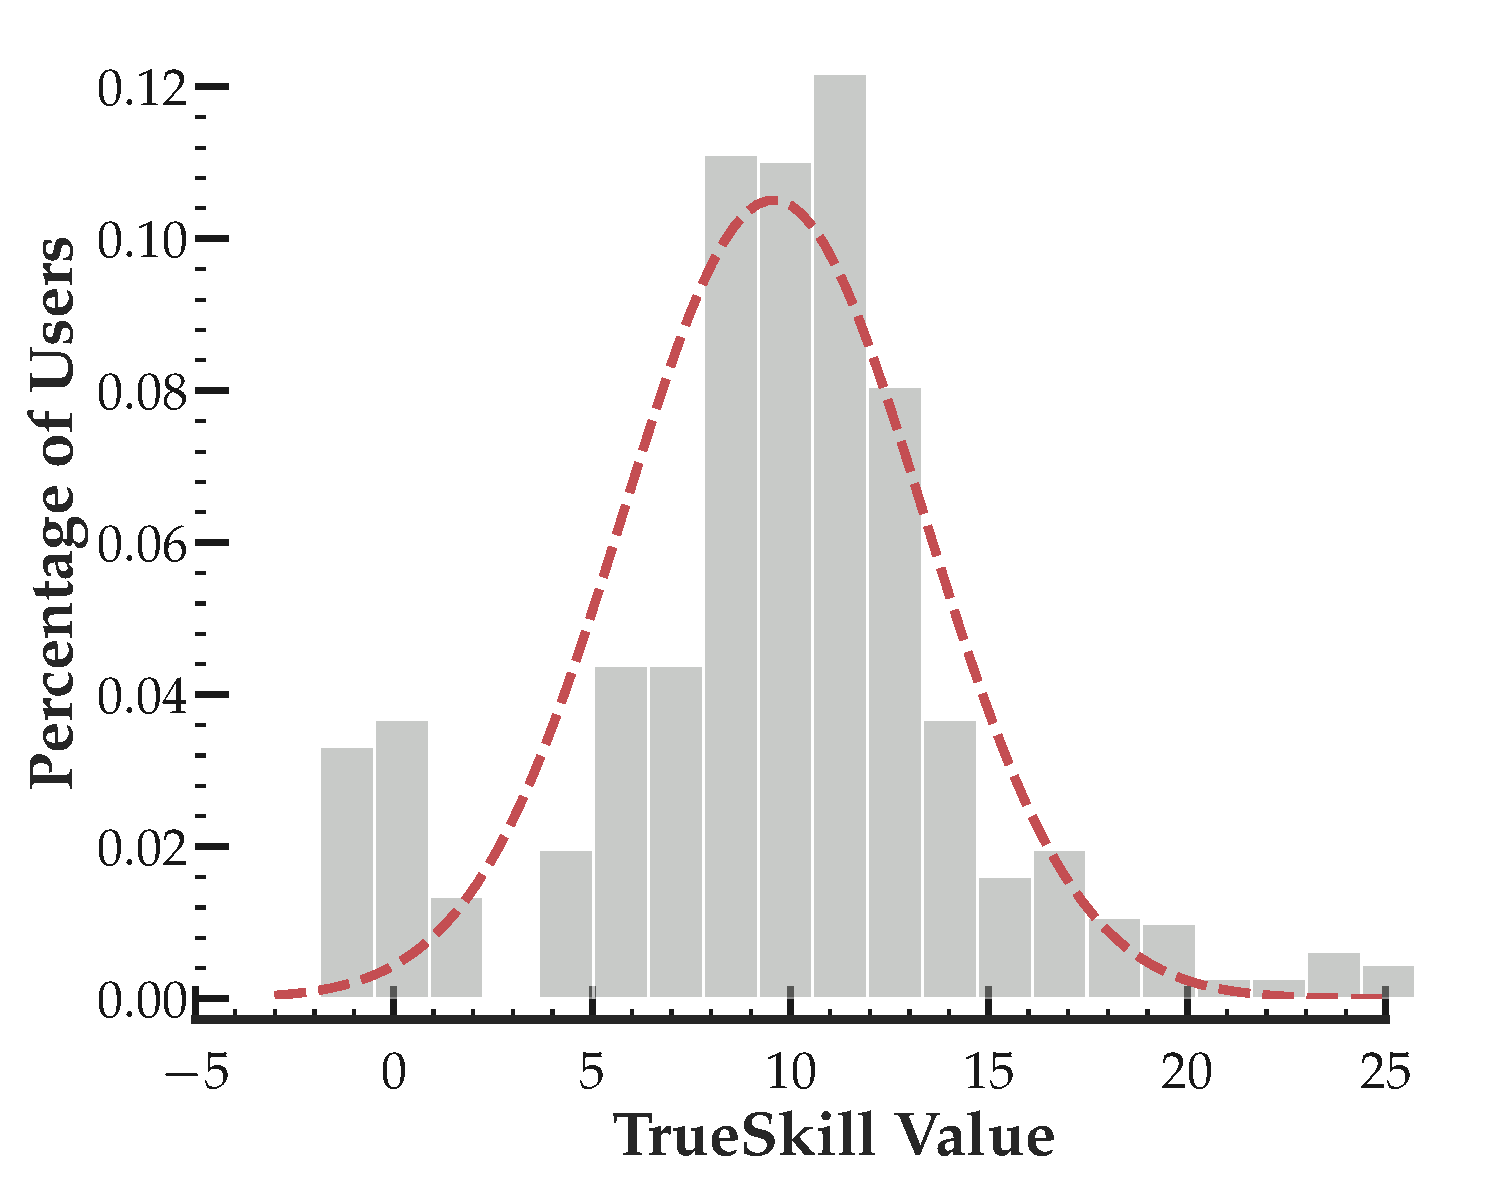
\includegraphics[height=5cm,width=\textwidth]{figures/TrueSkill}
    \caption{TrueSkill Distribution}\label{fig:trueskill}
  \end{subfigure}%
  \begin{subfigure}{0.4\textwidth}
    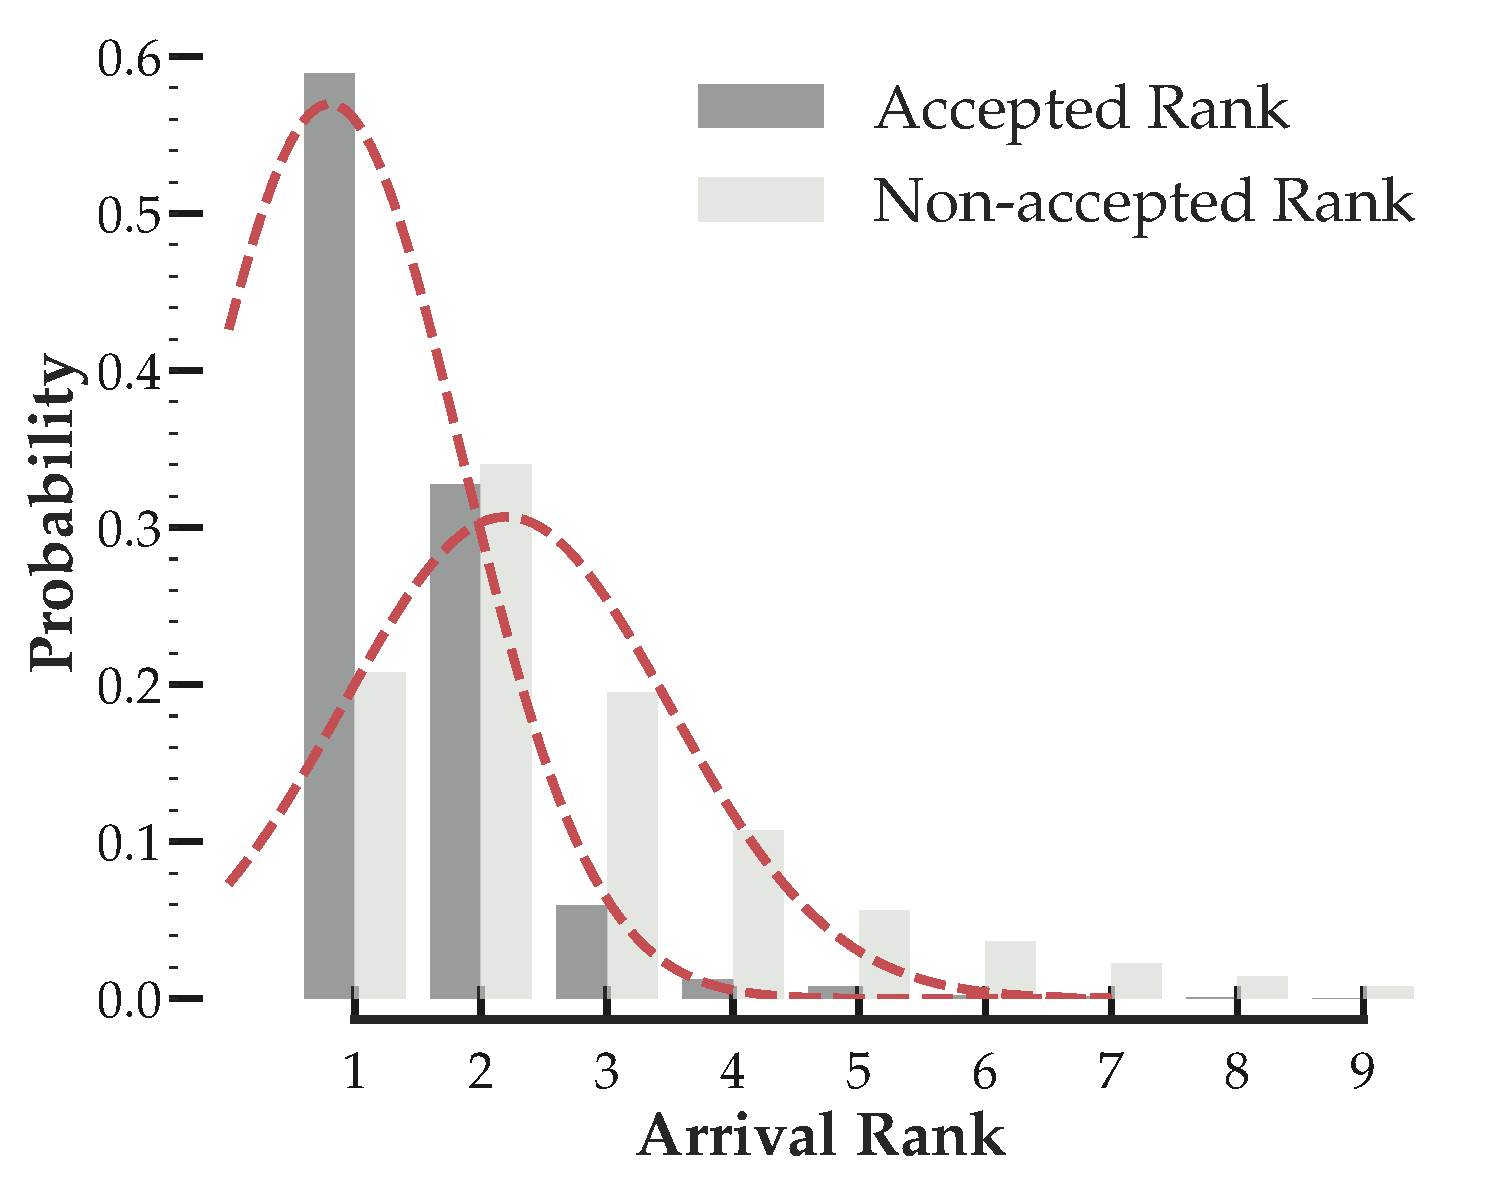
\includegraphics[height=5cm,width=\textwidth]{figures/ArrivalRank}
    \caption{ArrivalRank Distribution}\label{fig:arrival}
  \end{subfigure}
  \caption{\label{fig:similarcontrastsempirical} Distribution of the TrueSkill values of users and ArrivalRank of accepted answers and non-accepted answers for the movie StackExchange. Early answers are more likely to be accepted and variance of TrueSkill similarity across users is high.}
\end{figure}


Motivated by~\cite{Wu2016} and our empirical analysis (\cref{fig:similarcontrastsempirical}), we consider two different views that correspond to the similar contrast relation. The \emph{TrueSkill Similarity} view connects all answers authored by a user where her skill (computed via Bayesian TrueSkill~\cite{TrueSkill06})) differs from competitors by margin $\delta$. We capture both cases when the user is less or more skilled than her competitors. Under this view, we connect answers authored by a specific user, where the difference in his skill over peers is greater than margin $\delta$. Specifically, if the user authors answers $a, a'$ to questions $q, q'$, we create a link between $a$ and $a'$ if
\begin{align}
 \lvert S_{u,a} - S_{u, b} \rvert &> \delta; \forall b \in \mathcal{A}_(q) \\
 \lvert S_{u,a'} - S_{u, c} \rvert &> \delta; \forall c \in \mathcal{A}_(q')
\end{align}
where $S_{u,a}$ is the skill value for the user who authored answer $a$. Similarly, a link is created for the opposite case when difference is less than $-\delta$.
We estimate the user skill values with the TrueSkill rating system (\url{https://pypi.org/project/trueskill/}) computed from their historic performance in the community. TrueSkill values are normally distributed among users (\cref{fig:trueskill}).

In the \emph{Arrival Similarity} view, we connect answers across questions based on the similarity in the relative time of their arrival (posting timestamp).
The temporal arrival patterns of answers are correlated to their acceptance probabilities (\cref{fig:arrival}). For a specific user authoring answers $a, a'$ to questions $q, q'$, we establish a link between these answers if
\begin{align}
 \lvert T_{a} - T_{b} \rvert &> \gamma \times \max(T_{b}); \forall b \in \mathcal{A}_(q) \\
 \lvert T_{a'} - T_{c} \rvert &> \gamma \times \max(T_{c}); \forall c \in \mathcal{A}_(q')
\end{align}
where $T_{a}$ represents the relative time-gap between answer $a$ and the question $q$. Conversely, we create links when difference is less than $-\gamma \times \max(T_{b})$.

We hypothesize that a similar answering schedule indicates similar user confidence or skill across questions.
Notice that two Similar Contrast views have different edge ($E$) sets since the corresponding similarity functions are different. Notice also, that the two similarity function definitions are transitive.
 \footnote{One trivial way of establishing similarity is co-authorship i.e., connect all $(q,a)$ tuples of a user (probably on the same topic) across different questions.
Note that the accepted answer is labeled relative to the other answers. As the competing answers are different in each question, we can not trivially assume acceptance label similarity for all coauthored answers. In our experiments, co-authorship introduced a lot of noisy links in the graph leading to worse performance.}

\subsection{Generalized Views}
\label{sub:Generalized Views}
Now we present the general case of the induced view. First, notice that each of the three relation types that we consider---reflexive, contrastive, and similar---result in a graph $G_i = (V, E_i)$ comprising a set of cliques. The resulting set of cliques is not surprising, since all three relations presented here, are equivalence relations. Second, observe the semantics of how we select the tuple with the accepted answer. Within the three relations, we used two semantically different ways to assign the `accepted' answer label to a tuple. One way is to share the labels amongst all the vertices in the \textit{same clique} (used in the reflexive and the similar relations). The second is to \textit{assign label based on contrasts with other vertices} in the same clique. We can now state the organizing principle of our approach as follows.
\begin{quote}
  A generalized \textit{modular} framework: pick a meaningful equivalence relation on the $(q,a)$ tuples to induce graph comprising cliques and then apply specific label semantics within each clique.
\end{quote}

Equivalence relation results in a graph with a set of disconnected cliques. Then, within a clique, one could use application-specific semantics, different from two discussed in this paper, to label tuples as `accepted.'
Cliques have some advantages: they have well-defined graph spectra~\cite[p. 6]{Chung1997}; cliques allows for \textit{exact} graph convolution; parallelize the training as the convolution of a clique is independent of other cliques.

Thus, each strategy induces a graph $G_i=(V,E_i)$ using one of the three equivalence relations---reflexive, contrastive, and similar---and then applies one of the two semantics (`share the same label'; `determine label based on contrast').

\section{Induced Relational GCN}
\label{sec:gcn}
Now, we will encode the two label assignment mechanisms within a clique via a graph convolution. First, we briefly review Graph Convolution Networks (GCN) and identify some key concepts. Then, given the views $G_i$ for the four strategies, we show how to introduce label contrasts in~\Cref{subsec:contrast} followed by label sharing in~\Cref{subsec:similar}.

\subsection{Graph Convolution}
\label{subsec:graph}
Graph Convolution models adapt the convolution operations on regular grids (like images) to irregular graph-structured data $G = (V,E)$, learning low-dimensional vertex representations. If for example, we associate a scalar with each vertex $v \in V$, where $|V| = N$, then we can describe the convolution operation on a graph by the product of signal $x \in \mathbb{R}^N$ (feature vectors) with a learned filter $g_\theta$ in the fourier domain. Thus,
\begin{equation}
  g_\theta \ast x =  U \, g_\theta \, U^T x,
  \label{eq:basic_gcn}
\end{equation}
where, $\Lambda$ and $U$ are the eigenvalues and eigenvector of the normalized graph Laplacian, $L = I_N - D^{-\sfrac{1}{2}}AD^{\sfrac{1}{2}}$, and where $L = U \Lambda U^T$. $A$ denotes the adjacency matrix of a graph $G$ (associated with a view) with $N$ vertices. ~\Cref{eq:basic_gcn} implies a filter $g_\theta$ with $N$ free parameters, and requires expensive eigenvector decomposition of the adjacency matrix $A$. ~\citet{deferrard} proposed to approximate $g_\theta$, which in general is a function of $\Lambda$, by a sum of Chebyshev polynomials $T_k(x)$ up to the $k$-th order. Then,

\begin{equation}
  g_\theta \ast x \approx U \, \sum_{k=0}^K \theta_k T_k(\tilde{\Lambda}) \, U^T x \approx \, \sum_{k=0}^K \theta_k T_k(\tilde{L}) \, x,
  \label{eq:approx_gcn}
\end{equation}
where, $\tilde{\Lambda} = 2 \Lambda/ \lambda_{\max}- I_N$ are the scaled eigenvalues and $\tilde{L} = 2L/\lambda_{max} - I_N$ is the corresponding scaled Laplacian. Since $\tilde{L} = U \tilde{\Lambda} U^T$, the two equations are approximately equal.

The key result from~\citet{deferrard} is that~\Cref{eq:approx_gcn} implies $k$-hop localization---the convolution result depends only on the $k$-hop neighborhood. In other words,~\Cref{eq:approx_gcn}  is a $k$-hop approximation.

However, since we use equivalence relations in our framework that result in cliques, we can do an \textit{exact} convolution operation since vertices in a clique only have one-hop (i.e., $k=1$) neighbors (see lemma 5.2, \cite{Hammond2011}). The resulting convolution is linear in $L$ and now has only two filter parameters, $\theta_{0}$ and $\theta_{1}$ shared over the whole graph.
\begin{equation}
g_{\theta} * x = \theta_{0}x + \theta_{1}\left(L-I_{N} \right)x %\\
\label{eq:restrictk}
\end{equation}

We emphasize the distinction with~\citet{gcn} who approximate the~\citet{deferrard} observation by restricting $k=1$. They do so since they work on arbitrary graphs; since our relations result in views with cliques, we do not make any approximation by using $k=1$.

\begin{figure}[h]
  \centering
  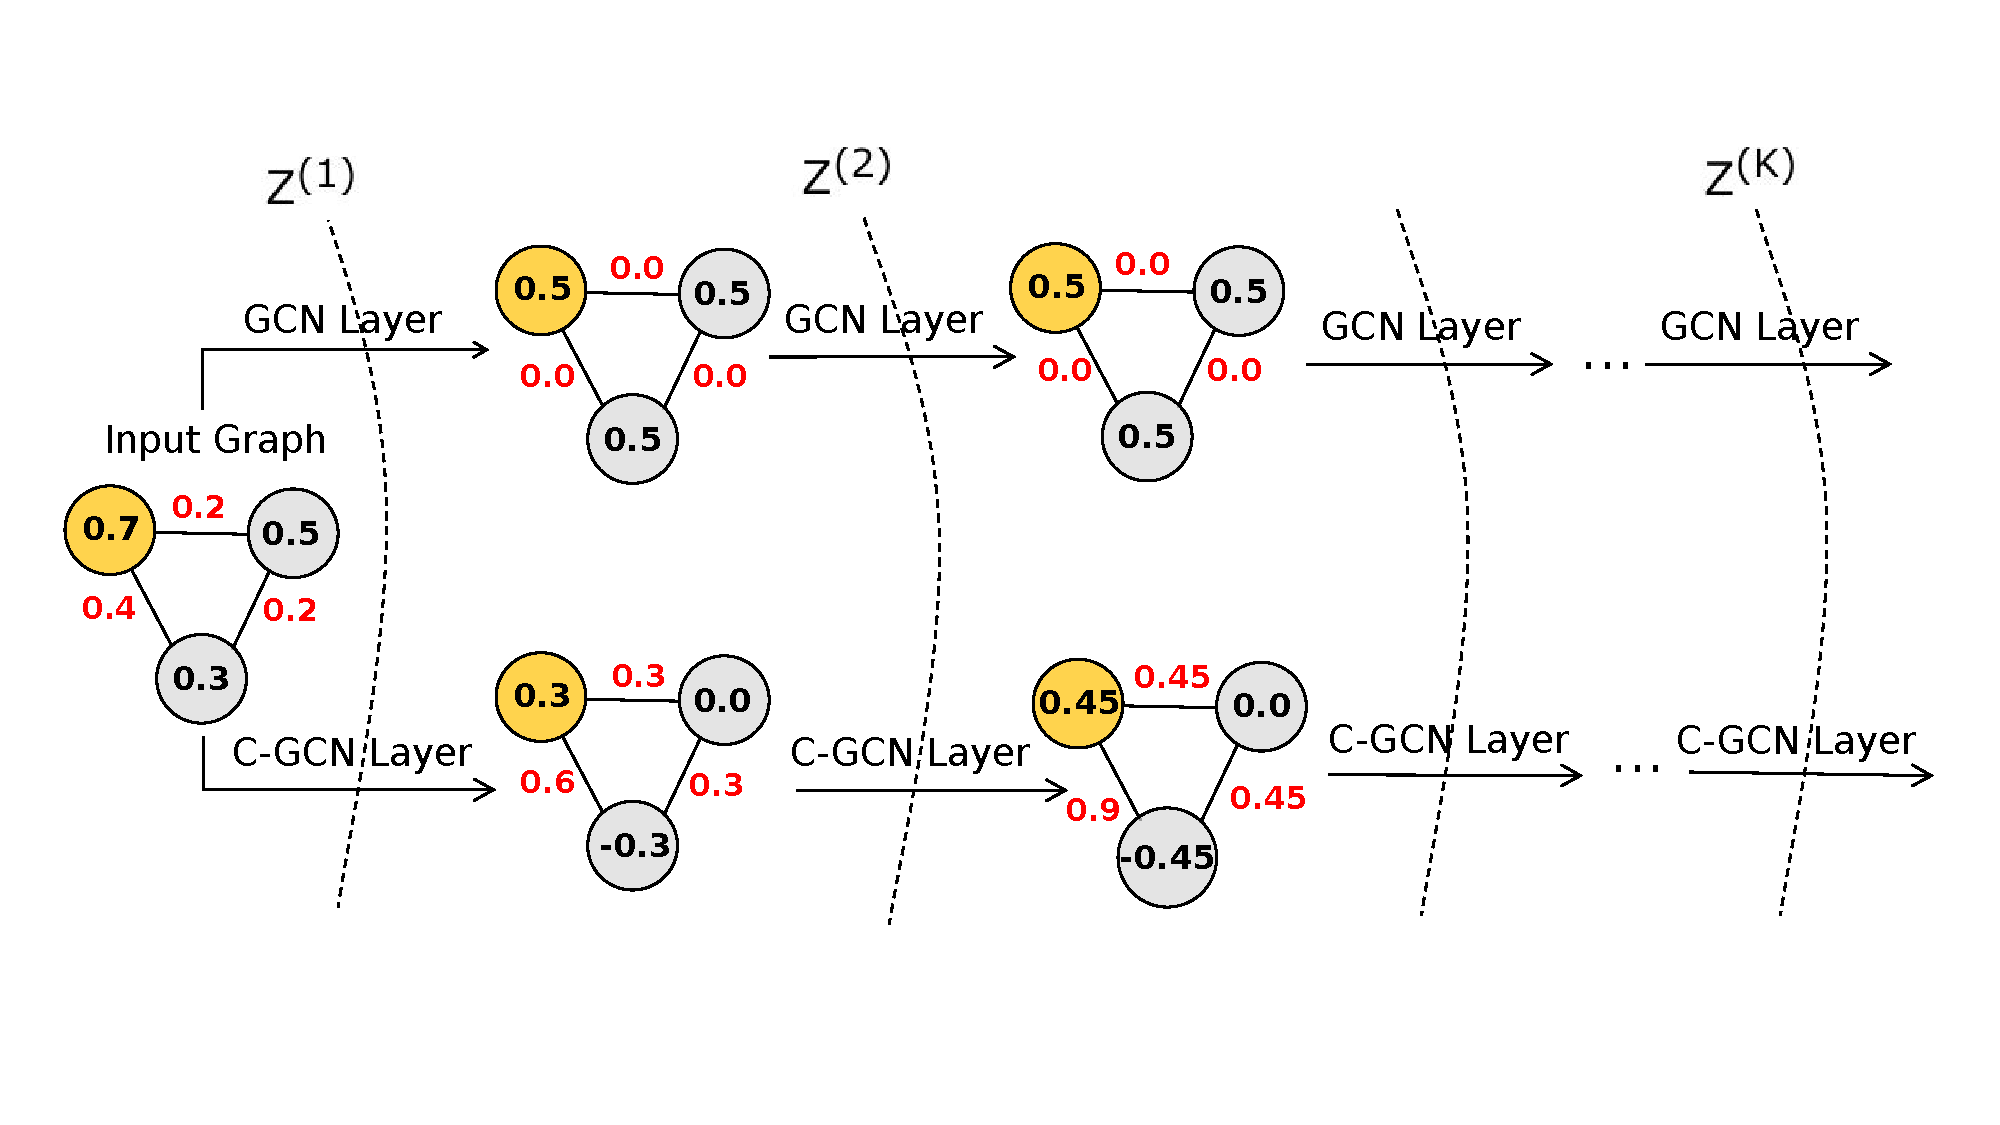
\includegraphics[scale=0.43]{figures/fig_contrast}
  \caption{\label{fig:contrast}Stylized example showing the convolution results of GCN and proposed Contrastive GCN for a question with three answers. Edge labels denote the feature difference while node labels denote the resulting feature value. The feature difference between neighboring nodes increases with each convolution layer for Contrastive GCN while GCN averages the feature values among nodes. }
\end{figure}

\subsection{Contrastive Graph Convolution}
\label{subsec:contrast}
Now, we show how to perform graph convolution to encode the mechanism of contrast, where label assignments for a tuple depend on the contrast with its neighborhood.

To establish contrast, we need to compute the \emph{difference} between the vertex's own features to its neighborhood in the clique. Thus we transform~\Cref{eq:restrictk} by setting $\theta = \theta_{0}$ = $\theta_{1}$, which essentially restricts the filters learned by the GCN. This transformation leads to the following convolution operation:
\begin{align}
g_{\theta} * x & =  \theta \left( I_N + L- I_{N} \right) x \\
g_{\theta} * x & =  \theta \left( I_N - D^{-\sfrac{1}{2}} A D^{-\sfrac{1}{2}}\right) x \label{eq:contrastdetail}
\end{align}

Notice that~\Cref{eq:contrastdetail} says that for example, for any vertex $u$ with a scalar feature value $x_u$, for a given clique with $n \geq 2$ vertices, the convolution operation computes a new value $\hat{x}_u$ for vertex $u$ as follows:
\begin{equation}
  \hat{x}_u = \theta \left ( x_u - \frac{1}{n-1} \sum_{v \in \mathcal{N}_u} x_v \right ).
\end{equation}
where $\mathcal{N}_u$ is the neighborhood of vertex $u$. Notice that since our equivalence relations construct cliques, for all vertices $u$ that belong to a clique of size $n$, $|\mathcal{N}_u| = n-1$.

When we apply the convolution operation in~\Cref{eq:contrastdetail} at each layer of GCN, output for the $k$-th layer is:

\begin{equation}
  \label{eq:contrast}
  \mathbf{Z}_c^{k} = \sigma \left( \left (I_N - D^{-\sfrac{1}{2}}A_cD^{\sfrac{1}{2}} \right) \mathbf{Z}_c^{k-1} \mathbf{W}_c^{k}\right)
\end{equation}
with $A_c$ denoting the adjacency matrix in the contrastive view. $\mathbf{Z}_c^{k} \in \mathbb{R}^{N \times d}$ are the learned vertex representations for each $(q,a)$ tuple under the contrastive label assignment. $N$ is the total number of tuples and $d$ refers to the dimensionality of the embedding space. $\mathbf{Z}^{k-1}$ refers to the output of the previous $(k-1)$-{th} layer, and $\mathbf{Z}^{0} = X$ where $X$ is the input feature matrix. $\mathbf{W}_c^{k}$ are the filter $\theta$ parameters learnt by the GCN; $\sigma( \cdot)$ denotes the activation function (e.g. ReLU, $\tanh$).

To understand the effect of~\Cref{eq:contrast} on a tuple, let us restrict our attention to a vertex $u$ in a clique of size $n$. We can do this since the convolution result in one clique is unaffected by other cliques. When we do this, we obtain:
\begin{equation}
  z_c^{k}(u) = \sigma \left(\left(z_c^{k-1}(u) - \frac{1}{n-1} \sum_{v \in \mathcal{N}_u} z_c^{k-1}(v) \right) \mathbf{W}_{c}^{k}\right). \label{eq:contrastrestrict}
  \end{equation}

Now consider a pair of contrasting vertices, $u$ and $v$ in the same clique of size $n$. Let us ignore the linear transform by setting $W_{c}^{k}=\mathbf{I}$ and set $\sigma(\cdot)$ to the identity function. Then we can easily verify that:
\begin{equation}
z_c^{k}(u) - z_c^{k}(v) = \underbrace{
  \left (1 + \frac{1}{n-1} \right )
  }_{\text{magnification}}
  \times
  \underbrace{
    \left ( z_c^{k-1}(u) - z_c^{k-1}(v) \right )
    }_{\text{contrast in previous layer}}, \label{eq:disccontrastsimple}
\end{equation}
where, $z_c^{k}(u)$ denotes the output of the $k$-th convolution layer for the $u$-th vertex in the contrastive view. As a result, each convolutional layer magnifies the feature contrast between the vertices that belong to the same clique. Thus, the contrasting vertices move further apart. We term this as \emph{Discriminative Feature Magnification} and~\Cref{eq:disccontrastsimple} implies that we should see higher magnification effect for smaller cliques.
An illustration is provided in the bottom part of the \cref{fig:contrast} with a uni-dimensional feature.

Contrasting nodes are shifted further apart by \cref{eq:contrast} improving their separability in the learned manifold (further discussion in \cref{ref:analysis}).

\subsection{Encoding Similarity Convolution}
\label{subsec:similar}
We next discuss how to encode the mechanism of sharing labels in a GCN. While label sharing applies to our similar contrast relation (two strategies: Arrival similarity; TrueSkill similarity, see~\Cref{sub:Induced Views}), it is also trivially applicable to the reflexive relation, where the label of the tuple only depends on itself. First, we discuss the case of similar contrasts.

\noindent
\textbf{Encoding Similar Contrasts:}
\label{sub:Encoding Similar Contrasts}
To encode label sharing for the two similar by contrast cases, we transform~\Cref{eq:restrictk} with the assumption $\theta = \theta_0 = -\theta_1$. Thus

\begin{equation}
g_{\theta} * x = \theta\left(I_{N} + D^{-\sfrac{1}{2}}AD^{-\sfrac{1}{2}}\right) x, \label{eq:similargcn}
\end{equation}

Similar to the ~\Cref{eq:contrastdetail} analysis, convolution operation in \Cref{eq:similargcn} computes a new value $\hat{x}_u$ for vertex $u$ as follows:
\begin{align}
  \hat{x}_u &= \theta \left ( x_u + \frac{1}{n-1} \sum_{v \in \mathcal{N}_u} x_v \right ).\\
  \hat{x}_u &= \theta \left ( \frac{n-2}{n-1} x_u + \frac{n}{n-1} \mu_x \right ).
\end{align}
That is, in the mechanism where we share labels in a clique, the convolution pushes the values of each vertex in the clique to the average feature value, $\mu_x = \frac{1}{n} \sum_{v \in \mathcal{N}_u \cup u} x_v$, in the clique.

When we apply the convolution operation in~\Cref{eq:similargcn} at each layer of GCN, output for the $k$-th layer:
\begin{equation}
  \label{eq:similar}
  \mathbf{Z}_s^{k} = \sigma \left( \left (I_N + D^{-\sfrac{1}{2}}A_sD^{\sfrac{1}{2}} \right) \mathbf{Z}_s^{k-1} \mathbf{W}_s^{k}\right)
\end{equation}
with $A_s$ denoting the adjacency matrix in the similar views.

We analyze the similarity GCN in a maner akin to~\Cref{eq:contrastrestrict} and we can easily verify that:

\begin{equation}
z_s^{k}(u) - z_s^{k}(v) = \underbrace{
  \left (1 - \frac{1}{n-1} \right )
  }_{\text{reduction}}
  \times
  \underbrace{
    \left ( z_s^{k-1}(u) - z_s^{k-1}(v) \right )
    }_{\text{contrast in previous layer}}, \label{eq:diffsimilar}
\end{equation}
where, $z_s^{k}(i)$ denotes the output of the $k$-th convolution layer for the $i$-th vertex in the similar view. As a result, each convolutional layer reduces the feature contrast between the vertices that belong to the same clique. Thus, the similar vertices move closer (see top part in ~\cref{fig:contrast}).

The proposed label sharing encoding applies to both similar contrast strategies (TrueSkill; Arrival). We refer to the corresponding vertex representations as $\mathbf{Z}_{ts}^{k}$ (TrueSkill), $\mathbf{Z}_{as}^{k}$ (Arrival).

\noindent
\textbf{Reflexive Convolution:}
\label{subsubsec:reflex}
We encode the reflexive relation with self-loops in the graph resulting in an identity adjacency matrix. This relation is the trivial label sharing case, with an independent assignment of vertex labels. Thus, the output of the $k$-th convolutional layer for the reflexive view, $\mathbf{Z}_r^{k}$ reduces to:
\begin{equation}
  \label{eq:reflexive}
  \mathbf{Z}_r^{k} = \sigma \left( I_N \mathbf{Z}_r^{k-1} \mathbf{W}_r^{k} \right)
\end{equation}
Hence, the reflexive convolution operation is equivalent to a feedforward neural network with multiple layers and activation $\sigma( \cdot )$.

\vspace{0.1in}
\noindent
Each strategy $S_i \in \mathbf{S}$ belongs to one of the three relation types---reflexive, contrastive and similarity, where $\mathbf{R}$ denotes the set of strategies of that relation type. $\mathcal{R} = \bigcup \mathbf{R}$ denotes the set of all relation types.
$\mathbf{Z}_i^K \in \mathbb{R}^{N X d}$ represents the $d$ dimensional vertex embeddings for strategy $S_i$ at the $K$-th layer. For each strategy $S_i$, we obtain a scalar score by multiplying $\mathbf{Z}_i^K$ with transform parameters $\widetilde{W}_i \in \mathbb{R}^{d \times 1}$.
The sum of these scores gives the combined prediction score, $\mathbf{H}_{\mathbf{R}} \in \mathbb{R}^{N X 1}$, for that relation type.
\begin{equation}
    \label{eq:score}
        \mathbf{H}_{\mathbf{R}} = \sum_{S_i \in \mathbf{R}} \mathbf{Z}_i^K \widetilde{W}_i^T
\end{equation}

In this section, we proposed Graph Convolutional architectures to compute vertex representations of each $(q,a)$ tuple under the four strategies.
In particular, we showed how to encode two different label assignment mechanisms---label sharing and determine label based on contrast---within a clique. The architecture that encodes label assignment based on contrast is a novel contribution; distinct from the formulations presented by~\citet{gcn} and its extensions~\cite{signedgcn, relationalGCN}. Prior convolutional architectures implicitly encode the label sharing mechanism (~\cref{eq:similargcn}); however, label sharing is unsuitable for contrastive relationships across vertices. Hence our architecture fills this gap in prior work.

\section{Aggregating Induced Views}
\label{sec:aggregation}
In the previous sections, we introduced four strategies to identify the accepted answer to a question. Each strategy induces a graph or relational view between $(q,a)$ tuples.
Each relational view is expected to capture semantically diverse neighborhoods of vertices. The convolution operator aggregates the neighborhood information under each view. The key question that follows is, \emph{how do we combine these diverse views in a unified learning framework?} Past work has considered multiple solutions:
\begin{itemize}
  \label{item:aggregator}
\item \textbf{Neighborhood Aggregation}: In this approach, they represent vertices by aggregating feature representations of it's neighbors across all views \cite{graphsage, relationalGCN}. Specifically, the final adjacency matrix is the sum of all the individual adjacency matrices of each view, i.e., $A = \sum_{S_i \in \mathbf{S}} A_i$. They, then, apply Graph Convolution Network to this updated Adjacency matrix.
\item \textbf{Stacking}: Multiple convolution layers stacked end-to-end (each potentially handling a different view) \cite{Stacking}. Specifically, they stacks all GCNs belonging to a view such that output of a lower GCN is fed as an input to the GCN directly above it. Thus, output from the last layer of GCN for view $i$, $Z_i^K$ s.t. $  S_i \in \textbf{S}$ will act as input features, $Z_j^0$ for some other view $j$ s.t. $S_j \in \{\textbf{S}-S_i \}$ if view $j$ is directly above the view $i$. In our experiments, we obtain the best performance by using the following order: Contrastive, Similarity by Contrast followed by Reflexive.
\item \textbf{Fusion}: Follows a multi-modal fusion approach~\cite{Fusion18}, where views are considered distinct data modalities. It treats each GCN as a separate model and appends the output from the final layer of each GCN i.e. $Z_i^K; \forall S_i \in \textbf{S}$ to the input of all the other GCN's, i.e. $Z_j^0 \forall S_j \in \textbf{S}-S_i$ along with the original features. Thus, the input of each GCN is linear in $\vert \textbf{S} \vert$.
\item \textbf{Shared Latent Structure}: Attempts to transfer knowledge across relational views (modalities) with constraints on the representations (e.g. \cite{DualGCN} aligns embeddings across views).
\end{itemize}

Ensemble methods introduced in \cite{relationalGCN} work on multi-relational edges in knowledge graphs. None of these approaches are directly suitable for our induced relationships. Our relational views utilize different label assignment semantics (label sharing within a clique vs. determine label based on contrast within a clique). In our label contrast semantics, we must achieve feature discrimination and label inversion between contrasting vertices, as opposed to label homogeneity and feature sharing in the label sharing case. Thus, aggregating relationships by pooling, concatenation, or addition of vertex representations fail to capture semantic heterogeneity of the induced views.
Further, data induced relations are uncurated and inherently noisy. Directly aggregating the learned representations via Stacking or Fusion can lead to noise propagation. We also expect views of the same relation type to be correlated.

\begin{figure}[tbh]
    \centering
    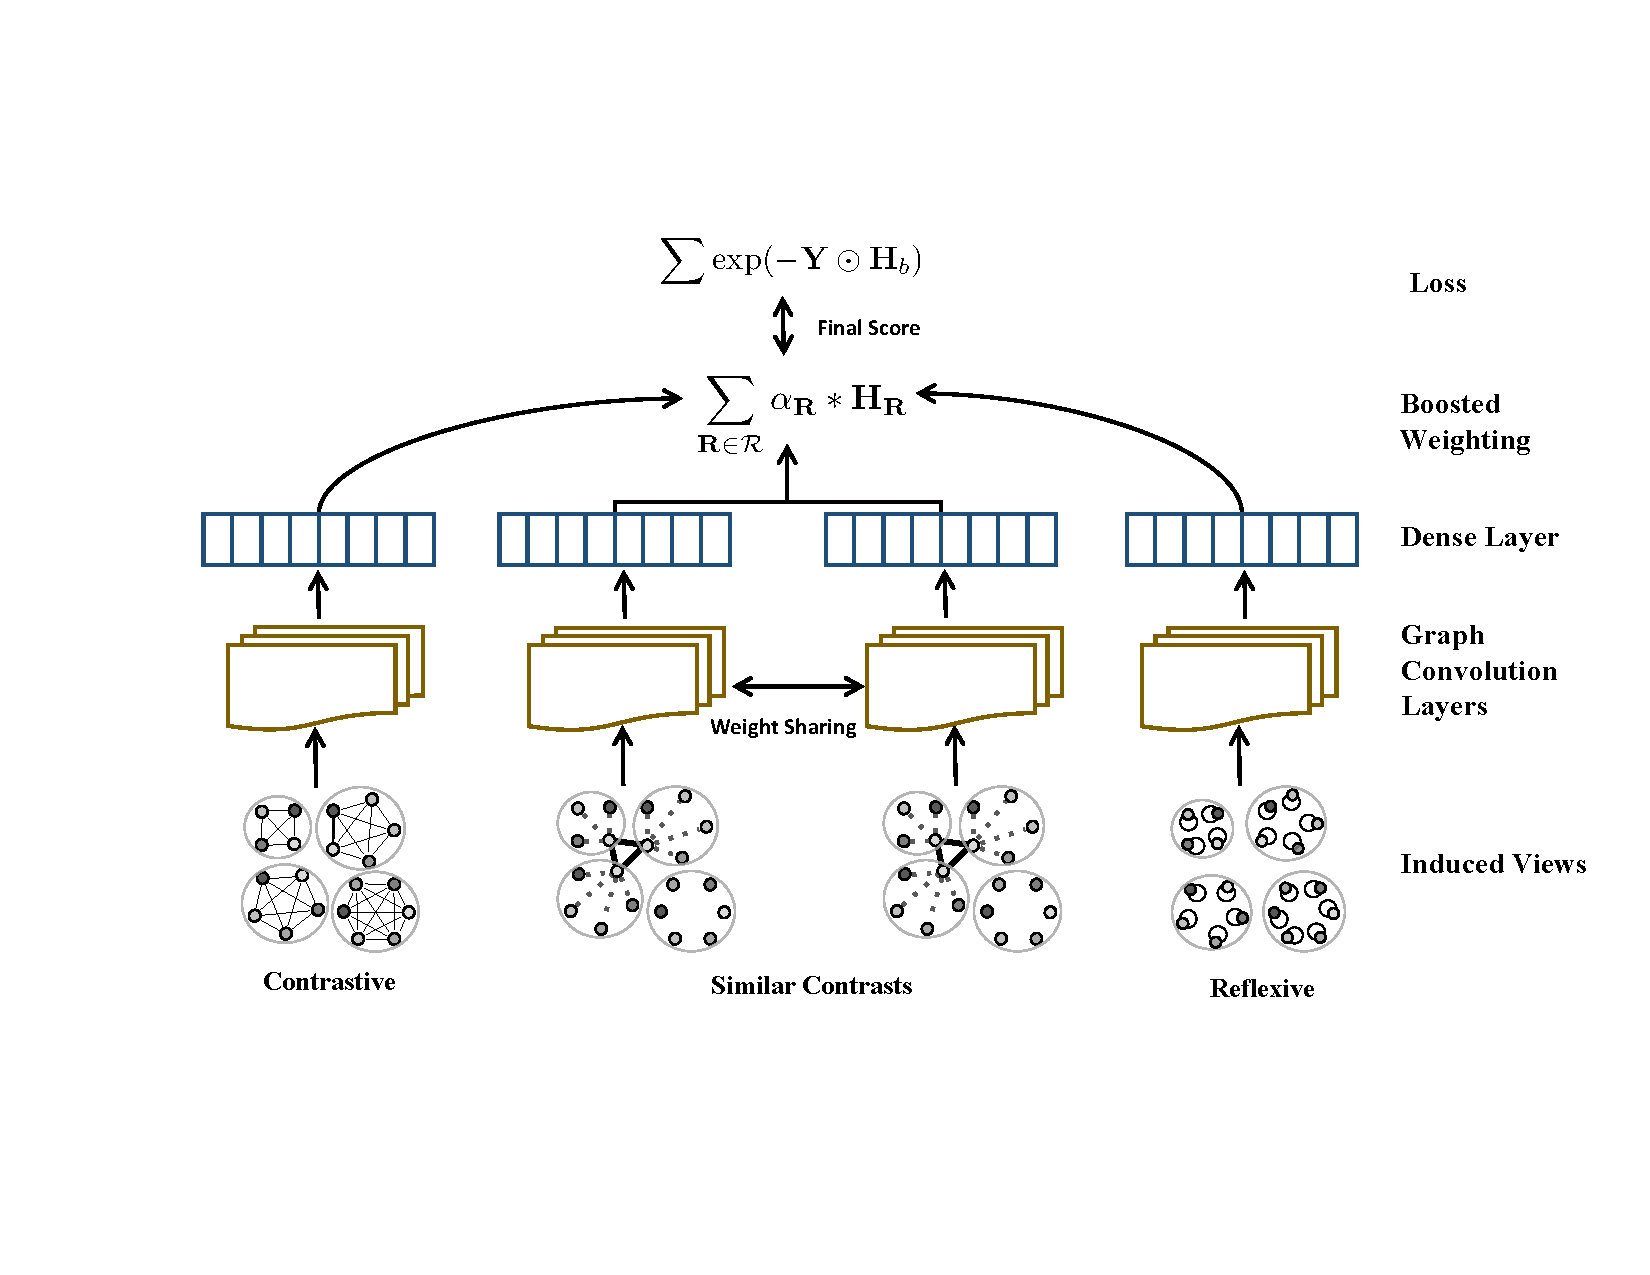
\includegraphics[scale=0.67]{figures/Architecture_new.pdf}
    \caption{\label{fig:adaboost} Schematic diagram of our proposed IR-GCN model.}
\end{figure}

We thus propose the following approach to aggregate information across relation types and between views of a relation type.

\noindent
\textbf{Cross-relation Aggregation}: We expect distinct relation types to perform well on different subsets of the set of $(q,a)$ tuples. We empirically verify this with the Jaccard overlap between the set of misclassified vertices under each relational view of a relation type on our dataset. Given $\mathbf{M}_A$ and $\mathbf{M}_B$, the sets of $(q,a)$ tuples misclassified by GCNs $A$ and $B$ respectively, the jaccard overlap is,
\begin{equation}
 \mathcal{J}_{A,B} = \frac{\mathbf{M}_A \cap \mathbf{M}_B}{\mathbf{M}_A \cup \mathbf{M}_B}
\end{equation}
The $\mathcal{J}_{A,B}$ values are as follows for the relational pairings: (Contrastive, TrueSkill Similarity) = 0.42, (Contrastive, Reflexive) = 0.44 and (Reflexive, TrueSkill Similarity) = 0.48. Relatively low values of the overlap metric indicate uncorrelated errors across the relations.

Gradient boosting techniques are known to improve performance when individual classifiers, including neural networks \cite{ncboost}, are diverse yet accurate. A natural solution then is to apply boosting to the set of relation types and bridge the weaknesses of each learner. We employ Adaboost \cite{adaboost} to combine relation level scores, $\mathbf{H}_{\mathbf{R}}$ (~\cref{eq:score}) in a weighted manner to compute the final boosted score, $\mathbf{H}_b \in \mathbb{R}^{N \times 1}$ representing all relation types (Line 12, ~\cref{alg:inference}). $\mathbf{Y} \in \mathbb{R}^{N X 1}$ denotes the acceptance label of all tuples. Note that an entry in $(\mathbf{Y} \odot \mathbf{H_{\mathbf{R}}}) > 0 $ when the accepted label of the corresponding $(q,a)$ tuple and sign of the prediction score, $sign(\mathbf{H_{\mathbf{R}}})$, of relation type $\mathbf{R}$ match and $< 0$ otherwise. Thus, the weights $\alpha_\mathbf{R}$ adapt to the fraction of correctly classified tuples to the misclassified tuples by the relation $\mathbf{R}$ (Line 9, ~\cref{alg:inference}).
The precise score computation is described in ~\cref{alg:inference}. We use the polarity of each entry in the boosted score, $sign(\mathbf{H}_b) \in \{-1,1 \}$, to predict the class label of the corresponding $(q,a)$ tuple. The final score is also used to create a ranked list among all the candidate answers, $a \in \mathcal{A}(q)$ for each question, $q \in \mathcal{Q}$. $L_{(q,a)}$ represents the position of candidate answer $a$ in the ranked list for question $q$.

\noindent
\textbf{Intra-relation Aggregation}: Gradient boosting methods can effectively aggregate relation level representations, but are not optimal within a relationship type (since it cannot capture shared commonalities between different views of a relation type). For instance, we should facilitate information sharing between the TrueSkill similarity and Arrival similarity views. Thus, if an answer is authored by a user with a higher skill rating and answered significantly earlier than other answers, its probability to be accepted should be mutually enhanced by both signals. Empirically, we also found True Skill and Arrival Similarity GCNs to commit similar mistakes ($\mathcal{J}_{TS,AS}$ = 0.66). Thus, intra-relation learning (within a single relation type like Similar Contrast) can benefit from sharing the structure of their latent spaces i.e., weight parameters of GCN.

\begin{algorithm}[tbh]
\caption{IR-GCN Boosted Score Computation}\label{alg:inference}
\begin{algorithmic}[1]
\Function{Forward}{$\mathbf{X}, \mathbf{Y}, \{A_i\}_{S_i \in \mathbf{S}}$}
  \State $\mathbf{H}_{b} \gets \mathbf{0} $
    \For{$\mathbf{R} \in \mathcal{R}$}
    \State $\{ \mathbf{Z}_i^K \}_{S_i \in \mathbf{R}} \gets Conv(\mathbf{X}, \{ A_i \}_{S_i \in \mathbf{R}})$
    \State \Comment{Equation  \ref{eq:contrast}, \ref{eq:similar}, \ref{eq:reflexive}}
    \State $\mathbf{H}_\mathbf{R} =\sum_{{S_i} \in \mathbf{R}} \mathbf{Z}_i^{K} \times \widetilde{\mathbf{W}}_i$ \Comment{Equation \ref{eq:score}}
    %\State $h_s = merge(h_{as}, h_{ts})$ \Comment{Equation \ref{eq:merge}}
    \State $ \mathbf{e}_{\mathbf{R}} \gets \exp({-\mathbf{Y} \odot \mathbf{H}_{b}})$
    \State \Comment{ $\odot \rightarrow \textit{Hadamard Product}$}
  \State $\alpha_\mathbf{R} \gets \dfrac{1}{2} \ln{\dfrac{\sum \mathbf{e}_{\mathbf{R}} \odot \mathbbm{1}\left((\mathbf{Y} \odot \mathbf{H}_{\mathbf{R}}\right) > 0)}{\sum \mathbf{e}_{\mathbf{R}} \odot \mathbbm{1}\left((\mathbf{Y} \odot \mathbf{H}_{\mathbf{R}}) < 0 \right) }}$
    \State \Comment{$\sum \rightarrow \textit{reduce-sum}$}
      \State \Comment{$\mathbbm{1}(.) \rightarrow \textit{element-wise Indicator function}$}
  \State    $\mathbf{H}_{b} \gets \mathbf{H}_{b} + \alpha_\mathbf{R} * \mathbf{H}_{\mathbf{R}}$ \Comment{Update boosted GCN}
    \EndFor
    \State \Return $\mathbf{H}_{b}$, $ \{ \mathbf{H}_{R} \}_{\mathbf{R} \in \mathcal{R}}$, $\{ \mathbf{Z}_{i}^{K} \}_{S_i \in \mathbf{S}}$
    \State \Comment{Boosted scores, Relation level scores,}
    \State \Comment{Each GCN vertex representations}
\EndFunction
\end{algorithmic}
\end{algorithm}

\noindent
\emph{Weight Sharing:} For multiple views representing a relation type (e.g., TrueSkill and Arrival Similarity), we train a separate GCN for each view but share the layer-wise linear-transforms $\mathbf{W}_i^{k}$ to capture similarities in the learned latent spaces.
Weight sharing is motivated by a similar idea explored to capture local and global views in \cite{DualGCN}. Although sharing the same weight parameters, each GCN can still learn distinct vertex representations as each view convolves over a different neighborhood and employ random dropout during training.
We thus propose to use an alignment loss term to minimize prediction difference between views of a single relation type\cite{reg}. The loss attempts to align the learned vertex representations at the \emph{last layer} $K$ (the loss term aligns pairs of final vertex representations, $\lvert\lvert \mathbf{Z}_i^{K} - \mathbf{Z}_{i'}^{K} \lvert\lvert \texttt{  }\forall\texttt{ } S_i, S_i' \in \mathbf{R}$). In principle, multiple GCNs augment performance of the relation type by sharing prior knowledge through multiple Adjacency matrices ($\mathbf{A}_i \texttt{  }\forall\texttt{ } S_i \in \mathbf{R}$).

\begin{algorithm}[!h]
\caption{IR-GCN Training}\label{alg:training}
\begin{algorithmic}[1]
\Require{Input Feature Matrix $X$, Acceptance labels for each tuple, $\mathbf{Y}$, Adjacency matrix of each view $\{A_i\}_{S_i \in \mathbf{S}}$ }
\Ensure{Trained Model i.e. Weight parameters $W_{i}^{1} \ldots W_{i}^{k}, S_i \in \mathbf{S}, \forall k \in [1, K]$ and transform parameters $\widetilde{W}_i$, $S_i \in \mathbf{S}$ }
\For{$t \gets 1$ to $\textit{num-epochs}$}
    \State $\mathbf{H}_b, \{ \mathbf{H}_{R} \}_{\mathbf{R} \in \mathcal{R}}, \{ \mathbf{Z}^{K}_{i} \}_{S_i \in \mathbf{S}}$$\gets \textsc{Forward}(X, Y, \{ A_i \}_{S_i \in \mathbf{S}})$
    \State \Comment{\Cref{alg:inference}}
    \For{ $\mathbf{R} \in \mathcal{R}$}

        \State $\mathcal L_b \gets \sum \exp({-\mathbf{Y} \odot \mathbf{H}_b}) + \gamma_1 \mathcal L_1(.) + \gamma_2 \mathcal L_2(.)$
    \State \Comment{$\sum \rightarrow \textit{reduce-sum}$}
  \State \Comment{$\odot \rightarrow \textit{Hadamard Product}$}
        \State $\mathcal L_{\mathbf{R}} \gets 0$
        \For{ $S_i \in \mathbf{R}$}
        \State $\mathcal L_{i} \gets \sum \exp({-\mathbf{Y} \odot \mathbf{H}_\mathbf{R}})$
    \State $\mathcal L_{\mathbf{R}} \gets \mathcal L_{\mathbf{R}} + \mathcal L_{i} + \frac{1}{2}\sum_{S_i' \neq S_i}\lvert\lvert \mathbf{Z}_{i}^K - \mathbf{Z}_{i'}^K \lvert\lvert $
    \EndFor
    \State $\mathcal L_b \gets \mathcal L_b + \lambda(t) \mathcal L_{\mathbf{R}}$
    \State    $W_i^{k} \gets  W_i^{k} + \eta_{\textsc{adam}} \frac{\partial \mathcal L_b}{\partial W_i^{k}} $ \Comment{$\forall k \in [1, K], \forall S_i \in \mathbf{R}$}
     \State    $\widetilde{W}_i \gets  \widetilde{W}_i +  \eta_{\textsc{adam}} \frac{\partial \mathcal L_b}{\partial \widetilde{W}_i}$ \Comment{$\forall S_i \in \mathbf{S}$}
    \EndFor
\EndFor
\end{algorithmic}
\end{algorithm}

\noindent
\textbf{Training Algorithm}: Algorithm \ref{alg:training} describes the training algorithm for our IR-GCN model. For each epoch, we first compute the aggregated prediction score $\mathbf{H}_{b}$ of our boosted model as described in \cref{alg:inference}. We use a supervised exponential loss $\mathcal{L}_b$ for training with elastic-net regularization (L1 loss - $\mathcal L_1(.)$ and L2 loss - $\mathcal L_2(.) $) on the graph convolutional weight matrices $\mathbf{W}_{\mathbf{i}}^{k} \texttt{  }\forall\texttt{ } S_i \in \mathbf{S}$ for each view. Note that we employ weight sharing between all views of the same relation type so that only one set of weight matrices is learned per relation. %The views in our training are Contrast (c), TrueSkill (ts), Arrival Similarity (as) and Reflexive view (r).

The exponential loss, $\mathcal{L}_{\mathbf{R}}$, for each relation type is added alternatingly to the boosted loss.
We apply an \emph{exponential annealing schedule}, $\lambda(t)$, i.e. a function of the training epochs ($t$), to the loss function of each relation. As training progresses and the boosted model learns to optimally distribute vertices among the relations, increase in $\lambda(t)$ ensures more emphasis is provided to the individual convolutional networks of each relation. Figure \ref{fig:adaboost} illustrates the overall architecture of our IR-GCN model.

\section{Experiments}
\label{sec:induced_experiments}
In this section, we first describe our dataset, followed by our experimental setup; comparative baselines, evaluation metrics, and implementation details. We then present results across several experiments to evaluate the performance of our model on merging semantically diverse induced-relations.

\subsection{Dataset}
We first evaluate our approach on multiple communities catering to different topics from a popular online Community Question Answer (CQA) platform, \emph{StackExchange\footnote{https://stackexchange.com/}}. The platform divides the communities into five different categories, i.e. Technology ($\mathbf{T}$), Culture/Recreation ($\mathbf{C}$), Life/Arts ($\mathbf{L}$), Science ($\mathbf{S}$) and Professional ($\mathbf{P}$).
For our analysis, we collect data from the ten largest communities from each of the five categories until March 2019, resulting in a total of 50 StackExchange communities.
The list of 50 StackExchange communities per category are;
\begin{itemize}
\item Technology: AskUbuntu, Server Fault, Unix, TEX, Electronics, Gis, Apple, Wordpress, Drupal, DBA
\item Culture/Recreation: English, Travel, RPG, Judaism, Puzzling, Bicycles, German, Christianity, BoardGames, History
\item Life/Arts: Scifi, DIY, Academia, Graphic Design, Money, Photo, WorldBuilding, Movies, Music, Law
\item Science: Stat, Physics, MathOverflow, CS, Chemistry, Biology, Philosophy, CS Theory, Economics, Astronomy

\item Professional/Business: Workplace, Aviation, Writers, Open source, Freelancing, CS Educators, Quant, PM, Parenting
\end{itemize}
In StackExchange, each questioner can mark a candidate answer as an "accepted" answer. We only consider questions with an accepted answer. Table \ref{tab:stats} shows the final dataset statistics.


\begin{table*}[h]
 \centering
 \begin{subtable}{\linewidth}
 \setlength{\tabcolsep}{3pt}
   \begin{tabular}{l | c c c | c c c | c c c }
  \toprule
  &  \multicolumn{3}{c}{{Technology}} &
  \multicolumn{3}{c}{{Culture/Recreation}} &
  \multicolumn{3}{c}{{Life/Arts}} \\
  & ServerFault & AskUbuntu & Unix & English & Games & Travel & SciFi & Home & Academia \\ \midrule
$\vert Q \vert$ & 61,873 & 41,192 & 9,207 & 30,616 & 12,946 & 6,782 & 14,974 & 8,022 & 6,442  \\
$\vert  \mathcal{A} \vert$ & 181,974 & 119,248 & 33,980 & 110,235 & 45,243 & 20,766 & 49,651& 23,956 & 23,837 \\
$ \vert U \vert$ & 140,676 & 200,208 & 84,026 & 74,592 & 14,038 & 23,304 & 33,754 & 30,698 & 19,088 \\
$ \mu (\vert  \mathcal{A}_q \vert) $ & 2.94 & 2.89 & 3.69 & 3.6 & 3.49 & 3.06 & 3.31 & 2.99 & 3.7 \\
   \bottomrule
 \end{tabular}%
\end{subtable}\vspace{8mm}

\begin{subtable}{\linewidth}
\centering
 \begin{tabular}{l | c c c | c c c}
\toprule
&
\multicolumn{3}{c}{{Science}} &
\multicolumn{3}{c}{{Professional/Business}}\\
& Physics & Maths & Statistics & Workplace & Aviation & Writing \\ \midrule
$\vert Q \vert$ &  23,932 & 18,464 & 13,773 & 8,118 & 4,663 & 2,932 \\
$\vert  \mathcal{A} \vert$ & 65,800 & 53,772 & 36,022 & 33,220 & 14,137 & 12,009 \\
$ \vert U \vert$ & 52,505 & 28,181 & 54,581& 19,713 & 7,519 & 6,918 \\
$ \mu (\vert  \mathcal{A}_q \vert) $ & 2.75 & 2.91 & 2.62 & 4.09 & 3.03 & 4.10 \\
 \bottomrule
\end{tabular}
\end{subtable}
 \caption{ \label{tab:stats}Dataset statistics for the top three Stack Exchange communities from five different categories. $\vert Q \vert$: number of questions; $\vert  \mathcal{A} \vert$: number of answers; $ \vert U \vert $: number of users; $ \mu (\vert  \mathcal{A}_q \vert) $: mean number of answers per question. Professional/Business communities have slightly more answers per question on average than others. Technology communities are the largest in terms of number of question out of the five categories.}
\end{table*}

For each $(q, a)$ tuple, we compute the following basic features:\\
\emph{Activity features :} View count of the question, number of comments for both question and answer, the difference between posting time of question and answer, arrival rank of answer (we assign rank 1 to the first posted answer) \cite{TianZL13}. \\
\emph{Text features :} Paragraph and word count of question and answer, presence of code snippet in question and answer (useful for programming based forums), word count in the question title.\\
\emph{User features :} Word count in user profile's Aboutme section for both users; one who is posting the question and the other posting the answer.

Time-dependent features like upvotes/downvotes of the answer and user features like reputation or badges used in earlier studies on StackExchange \cite{BurelMA16} are problematic for two reasons. First, we only know the aggregate values, not how these values change with time. Second, since these values typically increase over time, it is unclear if an accepted answer received the votes \emph{prior} to or \emph{after} an answer was accepted. Thus, we do not use such time-dependent features for our model and the baselines in our experiments.

\textbf{Reddit\footnote{https://www.reddit.com/}} is another popular CQA platform with subreddits similar to StackExchange communities. In particular, we focus on Ask* subreddits as they are primarily used to seek help from a community of experts and non-experts. In particular, we crawled data from /r/askscience (science forum), /r/AskHistorians (history forum), and /r/AskDocs (medical forum) until October 2017. We performed basic preprocessing and removed posts or comments with single word/URLs or missing author/title information. We also removed infrequent users who posted less than two comments.
Reddit has a hierarchical comment structure. For this paper, we treat first-level comments as potential answers to the question. Users in these subreddits can get verified by providing anonymized verification documents including certification numbers, contact information, etc. to the moderators. We denote these verified users as experts. We treat an expert's comment as equivalent to an accepted answer and only consider posts which have an expert answer for our experiments. We discard posts with multiple experts' comment as it is hard to objectively choose a winner.

\begin{table}[h]
\centering
\begin{tabular}{l  r r r r}
 \toprule
 Dataset & $\vert \mathcal{Q} \vert$ & $\vert \mathcal{A} \vert$ & $\vert \mathcal{U} \vert$ & $ \mu (\vert  \mathcal{A}_q \vert) $ \\  \midrule
 AskDocs & 11189 & 29207& 4530 & 2.61               \\
 AskHistorians & 15425 & 45586 & 11761 & 2.96                     \\
 AskScience & 37990 & 121278 & 32117 & 3.19                 \\
  \bottomrule
\end{tabular}
  \caption{Dataset statistics for the Ask* Reddit communities. $\vert Q \vert$: number of questions; $\vert  \mathcal{A} \vert$: number of answers; $ \vert U \vert $: number of users; $ \mu (\vert  \mathcal{A}_q \vert) $: mean number of answers per question.}
\end{table}

We employ 12 basic features for the Reddit dataset: \\
\emph{Activity features :} ArrivalRank of the answer, number of subsequent comments on the answer, number of other answers to the question, Upvotes and downvotes for both, question and answer.\\
\emph{Text features :} Word count of the question and answer

We employ post-vote features here as \cite{Gilbert:2013} showed that there is widespread under-provision of voting on Reddit, partially due to long comment threads. It can act as a weak signal for answer quality. Unlike the StackExchange, Reddit voting is not biased by publicly visible acceptance of answers to a question. Thus, votes ideally represent the independent judgment of the crowd.


\subsection{Experimental Setup}

\noindent
\textbf{Baselines} We compare against state-of-the-art feature-based baselines for answer selection and competing aggregation approaches to fuse diverse relational views of the dataset~\cite{DualGCN, relationalGCN}.

\noindent
\textit{Random Forest (RF)} \cite{BurelMA16, TianZL13} model trains on the feature set mentioned earlier for each dataset. This model is shown to be the most effective feature-based model for Answer Selection.

\noindent
\textit{Feed-Forward network (FF)} \cite{JendersKN16} is used as a deep learning baseline to learn non-linear transformations of the feature vectors for each $(q, a)$ tuple. This model is equivalent to our Reflexive GCN model in isolation.

\noindent
\textit{Dual GCN (DGCN)} \cite{DualGCN} trains a separate GCN for each view. In addition to the supervised loss computed using training labels, they introduce a regularizer to minimize mean squared error (MSE) between vertex representations of two views, thus aligning the learned latent spaces.
Formally,
For instance,
\begin{equation}
 \mathcal L_{reg}(Z_c, Z_{ts}) = \lVert \mathbf{Z}_c^K - \mathbf{Z}_{ts}^K \lVert
\end{equation}
computes the MSE loss between Contrastive and TrueSkill Similarity GCN.
\citet{DualGCN} proposed the model for two GCN representations and we extend it to four GCN with each GCN representing our relational view.
The Contrastive view is seen to exhibit the best performance in isolation. Thus, the DualGCN loss can be given by:

\begin{equation}
  \mathcal L  = \mathcal L_0 +  \lambda{(t)} \left( \sum_{S_i \in \mathbf{S}, S_i \neq c} \lVert \mathbf{Z}_c^K - \mathbf{Z}_i^K \lVert \right)
\end{equation}
where $\mathcal L_0$ represents the supervised loss and $\mathbf{Z}_c^K$ is the vertex representations of the Contrastive GCN.
The regularizer loss is similar to our intra-relation aggregation approach but assumes label and feature sharing across \emph{all} the views.

\noindent
\textit{Relational GCN (RGCN)} \cite{relationalGCN} combines the output representations of previous layer of each view to compute an aggregated input to the current layer, i.e.,
$\mathbf{Z}_i^{k-1}$ of layer $k-1$ of each view is used to compute an aggregated input to layer $k$.
Formally,

\begin{equation}
  \mathbf{Z}_{rgcn}^{k} = \sigma \left( \sum_{S_i \in \mathbf{S}} \mathbf{Z}_i^{k-1}\right)
\end{equation}
where $Z_{rgcn}$ is final output of this model at layer $k$ and $\sigma$ is the activation function.

We also report results for each view individually: Contrastive (C-GCN), Arrival Similarity (AS-GCN), TrueSkill Similarity (TS-GCN), and Reflexive (R-GCN) with our proposed IR-GCN model. We do not compare with other graph structure-based approaches to compute vertex representations \cite{DeepWalk, node2vec, Planetoid, LINE} as GCN is shown to outperform them \cite{gcn}. We also later compare with common aggregation strategies to merge neural representations discussed earlier in ~\cref{sec:aggregation}.

\noindent
\textbf{Evaluation Metric}
We randomly select 20\% of the questions, $\mathbf{T}_q \subset \mathcal{Q}$ to be in the test set. Then, subsequently all $(q,a)$ tuples such that $q \in \mathbf{T}_q$ comprise the set of test tuples or vertices, $\mathbf{T}$ . The rest of the vertices, along with their label information, is used for training the model.
We evaluate our model on two metrics, Accuracy and Mean Reciprocal Rank (MRR). Accuracy metric is widely used in vertex classification literature while MRR is popular for ranking problems like answer selection. Formally,
\begin{align}
Acc = \frac{1}{\vert \mathbf{T} \vert} \sum_{(q,a) \in  \mathbf{T} } \mathbbm{1} \left(  y_{(q,a)} \cdot h_b((q,a)) > 0 \right)
\end{align}
with $\cdot$ as the product and $\mathbbm{1}(.)$ as the indicator function. The product is positive if the accepted label and predicted label match and negative otherwise.
\begin{equation}
MRR = \frac{1}{\vert \mathbf{T}_q \vert} \sum_{q \in \mathbf{T}_q} \frac{1}{\sum_{a' \in \mathcal{A}(q)}  \mathbbm{1} \left(L_{(q,a)} < L_{(q,a')} \right)}
\end{equation}
 where
$L_{(q,a)}$ refers to the position of accepted answer $a$ in the ranked list for question $q$ \cite{Wang:2009}.

 \begin{table*}[!h]
\begin{threeparttable}[!h]
   \robustify\bfseries
   \centering
  \sisetup{
    table-figures-integer = 3,
    table-figures-decimal = 2,
    separate-uncertainty,
    table-figures-uncertainty = 1
  }
   %\setlength{\tabcolsep}{1pt}
   \begin{subtable}{\textwidth}
    %   \centering
   \resizebox{1\textwidth}{!}{
   %\centering
    \begin{tabular}{l|l l| l l | l l}
     \toprule
     \multirow{2}{*}{Method} &
        \multicolumn{2}{c}{{Technology}} &
       \multicolumn{2}{c}{{Culture/Recreation}} &
       \multicolumn{2}{c}{{Life/Arts}} \\
       &{Acc(\%)} & {MRR}&{Acc(\%)} & {MRR}&{Acc(\%)}& {MRR}\\
       \midrule
     {RF~\cite{BurelMA16, TianZL13}} & 66.78$\pm$0.023 & 0.683$\pm$0.043 & 72.5$\pm$0.018 & 0.626$\pm$0.050 & 72.71$\pm$0.049 & 0.628$\pm$0.089\\


     {FF~\cite{JendersKN16}} & 67.31$\pm$0.027 & 0.786$\pm$0.022 & 72.22$\pm$0.020 & 0.782$\pm$0.023\textbf{*} & 73.58$\pm$0.049 & 0.780$\pm$0.034 \\
     {DGCN~\cite{DualGCN}} & 70.70$\pm$0.022 & 0.782$\pm$0.017 & 75.22$\pm$0.017 & 0.771$\pm$0.028 & 76.73$\pm$0.034 &0.784$\pm$0.038 \\
     {RGCN~\cite{relationalGCN}} & 54.40$\pm$0.045 & 0.673$\pm$0.045 & 60.39$\pm$0.016 & 0.645$\pm$0.042 & 59.97$\pm$0.043 & 0.654$\pm$0.054 \\
     \cmidrule(lr){1-1}\cmidrule(lr){2-7}
     {AS-GCN} & 67.76$\pm$0.032 &0.775 $\pm$0.015 & 73.05 $\pm$0.021 & 0.763$\pm$0.025 &73.79 $\pm$0.048 & 0.776$\pm$0.042 \\
     {TS-GCN} & 66.87$\pm$0.032 & 0.779$\pm$0.018 & 72.16$\pm$0.023 & 0.764$\pm$0.023 & 72.02$\pm$0.061 & 0.765$\pm$0.048 \\
     {C-GCN} & 71.64$\pm$0.022\textbf{*} & 0.790$\pm$0.015\textbf{*}& 76.18$\pm$0.017\textbf{*}& 0.781$\pm$0.024 & 77.37$\pm$0.034\textbf{*}& 0.788$\pm$0.040\textbf{*} \\
     {IR-GCN} & \bfseries 73.96$\pm$\bfseries0.023 & \bfseries0.794$\pm$\bfseries0.014 & \bfseries 78.61$\pm$\bfseries0.018 & \bfseries0.790$\pm$\bfseries0.025 & \bfseries79.21$\pm$\bfseries0.032 & \bfseries0.800$\pm$\bfseries0.037 \\
     \bottomrule
   \end{tabular}
   }
   \end{subtable}\vspace{8mm}
   \begin{subtable}{\textwidth}
   \resizebox{0.73\textwidth}{!}{
   \begin{tabular}{l|l l| l l }
    \toprule
    \multirow{2}{*}{Method} &
      \multicolumn{2}{c}{{Science}} &
      \multicolumn{2}{c}{{Professional/Business}}\\
      & {Acc(\%)} & {MRR}&{Acc(\%)} & {MRR}\\
      \midrule
    {RF~\cite{BurelMA16, TianZL13}} & 68.09$\pm$0.024 & 0.692$\pm$0.049 & 74.72$\pm$0.044 & 0.5951$\pm$0.081\\
    {FF~\cite{JendersKN16}} & 67.87$\pm$0.024 & 0.800$\pm$ 0.028 & 74.63$\pm$0.040 & 0.759$\pm$0.049\\
    {DGCN~\cite{DualGCN}} & 71.45$\pm$0.023\textbf{*} & 0.791$\pm$0.035 & 76.86$\pm$0.031 & 0.751$\pm$0.046\\
    {RGCN~\cite{relationalGCN}} & 58.65$\pm$0.054 & 0.682$\pm$0.042 &63.02$\pm$0.038 & 0.657$\pm$0.061\\
    \cmidrule(lr){1-1}\cmidrule(lr){2-5}%\cmidrule(lr){12-21}
    {AS-GCN} & 66.93$\pm$0.045 & 0.788 $\pm$0.028 & 74.99$\pm$0.045 &0.742 $\pm$0.047\\
    {TS-GCN} & 65.90$\pm$0.042 & 0.790$\pm$0.031 & 74.17$\pm$0.046 &0.747$\pm$0.044\\
    {C-GCN} & 70.81$\pm$0.042 & 0.800$\pm$0.032\textbf{*}& 77.57$\pm$0.038\textbf{*} & 0.768$\pm$0.034\textbf{*}\\
    {IR-GCN} & \bfseries74.98$\pm$\bfseries0.021 & \bfseries0.808$\pm$\bfseries0.028 & \bfseries80.17$\pm$\bfseries0.026 & \bfseries0.785$\pm$\bfseries0.032\\
    \bottomrule
  \end{tabular}
  }
  \end{subtable}
   \begin{tablenotes}
       \footnotesize
       \item[*] DGCN stands for DualGCN, RGCN stands for RelationalGCN, and IR-GCN stands for Induced Relational GCN.
   \end{tablenotes}
   \caption{\label{tab:stackacc} Accuracy and MRR values for StackExchange with state-of-the-art baselines. Our model outperforms by at least 4\% in Accuracy and 2.5\% in MRR. Contrastive GCN performs best among individual views. The model with $*$ symbol has the second-best performance among all other models. Our model shows statistical significance at level 0.01 overall second best model on single tail paired t-test.}
   \end{threeparttable}
 \end{table*}


\noindent
\textbf{Implementation Details}
We implemented our model and the baselines in Pytorch. We use ADAM optimizer \cite{ADAM} for training with 50\% dropout to avoid overfitting. We use four hidden layers in each GCN with hidden dimensions 50, 10, 10, 5, respectively, and ReLU activation. The coefficients of $\mathcal{L}_1$ and $\mathcal{L}_2$ regularizers are set to $\gamma_1 = 0.05$ and $\gamma_2 = 0.01$ respectively. For TrueSkill Similarity, we use margin $\delta = 4$ to create links, while for Arrival similarity, we use $\delta = 0.95$.
We implement a mini-batch version of training for large graphs where each batch contains a set of questions and their associated answers.  This mini-batch version is equivalent to training on the whole graph as we have disconnected cliques.


\subsection{Performance Analysis}
Table \ref{tab:stackacc} shows impressive gains over state-of-the-art baselines for all the five categories of StackExchange. We report mean results for each category obtained after 5-fold cross-validation on each of the communities. Our induced-relational GCN model beats best performing baseline by 4-5\% on average in accuracy. The improvement in MRR values is around 2.5-3\% across all categories. Note that MRR is based only on the rank of the accepted answer, while accuracy is based on correct labeling of \emph{both} accepted and non-accepted answers.

\begin{figure}[h]
  \centering
  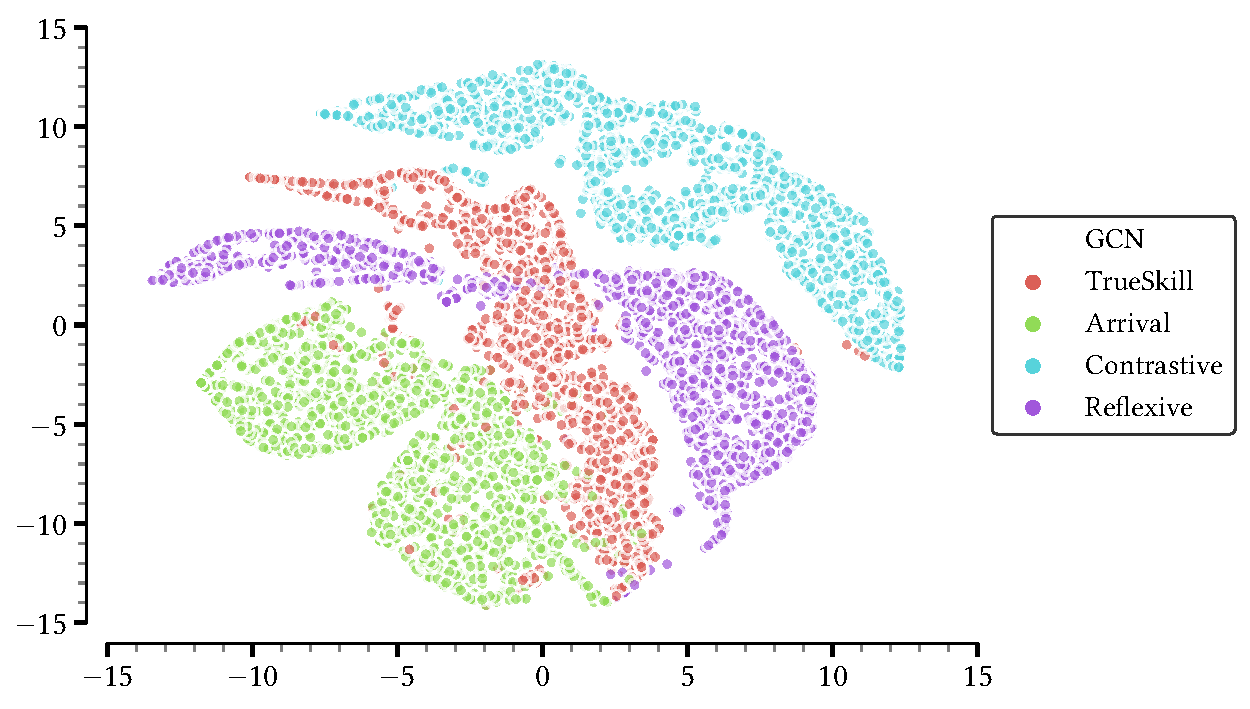
\includegraphics[scale=0.5]{figures/sne_plot.pdf}
  \caption{\label{fig:sne} t-stochastic neighbor embedding (t-SNE) \cite{sne} distributions of the learned vertex representations by our model for Chemistry StackExchange. Each view learns a distinct vertex representation. Best viewed in color.}
\end{figure}

Among individual views, Contrastive GCN performs best on all the communities. It even beats the best performing baseline DualGCN that uses all the relational views. Note that the contrastive view compares between the candidate answers to a question and uses our proposed contrastive modification to the convolution operation. Arrival Similarity follows Contrastive and then Reflexive. The superior performance of the Arrival Similarity view shows that early answers tend to get accepted and vice versa. It indicates that users primarily use CQA forums for quick answers to their queries. Also, recall that Reflexive predicts each vertex's label independent of other answers to the same question. Thus, the competitive performance of the Reflexive strategy indicates that vertex's features itself are well predictive of the label. TrueSkill Similarity performs at par or slightly worse than Reflexive. \Cref{fig:sne} presents t-SNE distributions \cite{sne} of the learned vertex representations ($\mathbf{Z}_i^K$) of our model applied to Chemistry StackExchange from Science category. Note that each view, including two views under Similar Contrast relation, learns a distinct vertex representation. Hence, all views are essential and contribute to our final performance.

Out of the baseline graph ensemble approaches, DualGCN performs significantly better than RelationalGCN by an average of around 26\% for all categories. Recall that in the RelationalGCN model, the convolution output of each view is linearly combined to compute the final output. Linear combination works well for knowledge graphs as each view can be thought of as a feature, and then it accumulates information from each feature. DualGCN is similar to our approach and trains different GCN for each view and later merges their results. However, it enforces similarity in vertex representations learned by each view. This restriction is not suitable for our induced-relationships as they are semantically different (contrastive captures contrast in features vs. similarity enforces label sharing).

\begin{table}[tbh]
  \robustify\bfseries
  \centering
  \sisetup{
    table-figures-integer = 3,
    table-figures-decimal = 2,
    separate-uncertainty,
    table-figures-uncertainty = 1
  }
  \begin{tabular}{l| c c c c c c}
    \toprule
    \multirow{2}{*}{{Method}} &
      \multicolumn{2}{c}{{AskDocs}} &
      \multicolumn{2}{c}{{AskHistorians}} &
      \multicolumn{2}{c}{{AskScience}} \\
      & {Acc (\%)} & {MRR} & {Acc(\%)} & {MRR} & {Acc(\%)} & {MRR} \\
      \midrule
    RF~\cite{BurelMA16, TianZL13} & 59.35 & 0.698 & 65.62 & 0.709 & 65.87 & 0.706  \\
    FF~\cite{JendersKN16} & 62.30 & 0.715 & 67.89 & 0.7302 & 68.99 & 0.713  \\
    DGCN~\cite{DualGCN} & 77.54 & 0.790 & 80.49 & 0.805 & 75.57 & 0.821 \\
    RGCN~\cite{relationalGCN} & 57.98 & 0.667 & 64.56 & 0.684 & 62.42 & 0.642 \\
    \midrule
    AS-GCN & 76.53 & 0.794 & 80.70 & 0.781 & 78.14 & 0.797 \\
    TS-GCN & 84.44 & 0.861 & 90.95 & 0.829 & 87.61 & 0.822 \\
    C-GCN & 67.39 & 0.753 & 70.57 & 0.744 & 71.11 & 0.769 \\
    IR-GCN & \textbf{87.60} &  \textbf{0.896} &  \textbf{93.81} &  \textbf{0.851} &  \textbf{89.11} &  \textbf{0.837} \\
    \bottomrule
  \end{tabular}
  \caption{\label{tab:reddit} Accuracy and MRR values for Ask\* Reddits. Our model significantly outperforms by 16\% in Accuracy and 7\% in MRR. TrueSkill Similarity performs best among individual IR-GCNs.}
\end{table}

Table \ref{tab:reddit} shows performance gains over the state-of-art baselines for the Reddit dataset. All results are reported after 5-fold cross-validation. Our model improves by 16\% on average in accuracy over the baselines for Reddit. The improvement in MRR is at an average increase of 7\% than the baseline higher than for StackExchange.

Among individual views, for Reddit, there is a considerable difference in performance for each view. TrueSkill Similarity performs much better, followed by Arrival Similarity and Contrastive. Reflexive GCN performs the worst for Reddit as it predicts each node's label independent of answers to the same question.

Out of the baseline graph ensemble approaches, DualGCN and RelationalGCN, similar to StackExchange, DualGCN consistently performs better than RelationalGCN by an average of around 3\% for Reddit.

\section{Discussion}
\label{sec:discussion}
In this section, we first evaluate the importance of each relational view for our boosted model. We then compare with approaches proposed to merge neural networks in general in other domains. We then illustrate \emph{discriminative magnification effect} in detail and study the robustness of our model to training label sparsity.  We also extend our proposed approach to include textual features and compare it with a text-based model. Finally, we provide a theoretical analysis of performance gains of our Contrastive GCN model and provide limitations of our approach.

\subsection{Ablation Study on Relation Types}
\begin{table}[h]
 \centering
  \robustify\bfseries
  \begin{tabular}{l | c | c| c| c|c | c}
    \toprule
       {\{ Relation Type\}} &
        {Tech} &
        {Culture} &
        {Life} &
        {Sci}&
        {Business} & {AskDocs}\\
      \midrule
      C & 71.23 &75.90 &78.71&72.99 & 76.85 & 67.39\\
    \{ TS, AS \} & 67.86 &74.15 &75.75&65.80& 76.13 & 84.57 \\
    R & 68.30 & 73.35 & 76.57 & 67.40 & 75.76 & 62.30\\
    \{TS, AS \} + R & 69.28 & 75.50 &76.41 &70.11 &77.90 & 86.34  \\
    C + R & 73.04 & 77.66 & 80.25 &73.72 & 80.04 & 70.02\\
    C + \{ TS, AS \} & 72.81 & 78.04 & 81.41 & 72.19 & 80.15 & 86.99\\
    C + \{ TS, AS \} + R & \bfseries 73.87 & \bfseries 78.74 & \bfseries 81.60&  \bfseries74.68&  \bfseries80.56 & \bfseries 87.60\\
    \bottomrule
  \end{tabular}
  \caption{\label{tab:relation} 5-fold Accuracy (in \%) comparison for different combination of relation types for our boosted model. Contrastive and Similar Contrast relations together performs similar to the final model.}
\end{table}
We present results of an ablation study with different combination of relation types (Contrastive, Similar and Reflexive) used for IR-GCN model in Table \ref{tab:relation}. We conducted this study on the biggest community from each of the five categories, i.e., ServerFault (Technology), English (Culture), Science Fiction (Life), Physics (Science), Workplace (Business). We also report results for AskDocs subreddit.
Similar Contrast relation (TrueSkill and Arrival) used in isolation perform the worst among all the variants. Training Contrastive and Similar Contrast relation together in our boosted framework performs similar to our final model. Reflexive GCN contributes the least as it does not consider any neighbors.

\subsection{Aggregator Architecture Variants}
\label{sec:agg}
We compare our gradient boosting based aggregation approach with other popular methods used in literature to merge different neural networks discussed in \cref{item:aggregator}.
\begin{table}[h]
  %\small
  \centering
  \robustify\bfseries
  \begin{tabular}{l | c | c| c| c|c|c}
    \toprule
    {Method} &
    {Tech} &
    {Culture} &
    {Life} &
    {Sci}&
    {Business} & {AskDocs}\\
      \midrule
    Stacking~\cite{Stacking} &68.58 & 74.44 & 79.19 & 70.29 &75.50 & 85.40 \\
    Fusion~\cite{Fusion18}  &72.30 &77.25 & 80.79 & 73.91 &79.01 & 86.33\\
    NeighborAgg~\cite{graphsage, relationalGCN}  &69.29 &74.28 & 77.94 & 68.42 &78.64 & 86.00  \\
    IR-GCN & \bfseries 73.87 & \bfseries 78.74 & \bfseries 81.60&  \bfseries74.78&  \bfseries80.56 & \bfseries 87.60\\
    \bottomrule
  \end{tabular}
  \caption{\label{tab:agg} 5-fold Accuracy (in \%) comparison of different aggregator architectures. These architectures perform worse than Contrastive GCN for StackExchange. Fusion performs similarly but is computationally expensive.}
\end{table}

Table \ref{tab:agg} reports the accuracy results for these aggregator variants as compared to our model. Our method outperforms all the variants with Fusion performing the best.  This superior performance affirms that existing aggregation models are not suitable for our problem. Note that these approaches perform worse than even Contrastive GCN except Fusion. The fusion approach performs similarly to our approach but is computationally expensive as the input size for each view is linear in the number of all views in the model.

\subsection{Discriminative Magnification effect}

\begin{figure}[tbh]
  \centering
  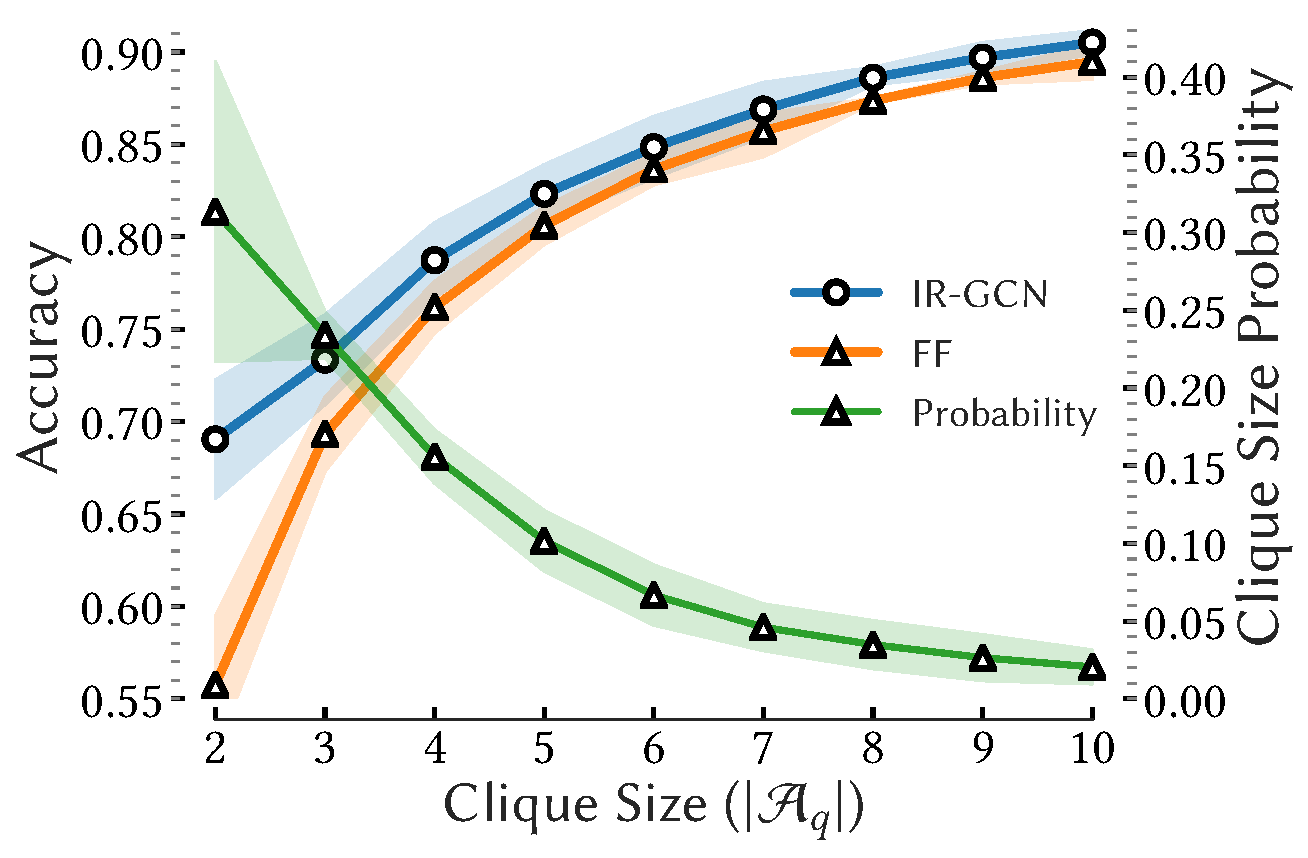
\includegraphics[scale=0.5]{figures/clique_acc.pdf}
  \caption{\label{fig:clique} Accuracy of our IR-GCN model compared to the FF model with varying clique size (i.e. number of answers to a question, $\vert \mathcal{A}_q \vert$) for Contrastive view .
We report averaged results over the largest community of all categories. Our model performs much better for smaller cliques, and the effect diminishes for larger cliques (\cref{eq:contrast}). 80\% of the questions have $< 4$ answers.}
\end{figure}

We show that due to our proposed modification to the convolution operation for contrastive view, we achieve \emph{Discriminative Magnification effect} (\cref{eq:contrast}). Note that the difference is scaled by Clique size ($1 + 1/n-1$), i.e. number of answers to a question, $\vert \mathcal{A}_q \vert$. Figure \ref{fig:clique} shows the accuracy of our IR-GCN model as compared to the FeedForward model with varying clique size. Recall that the FeedForward model predicts node labels independent of other nodes and is not affected by clique size. We report average results over the same five communities as above. We can observe that increase in accuracy is much more for lower clique sizes (13\% improvement for $\vert \mathcal{A}_q \vert = 2$ and 4\% for $\vert \mathcal{A}_q \vert = 3$ on average). The results are almost similar for larger clique sizes. In other words, our model significantly outperforms the FeedForward model for questions with fewer candidate answers. However, around 80\% of the questions have very few answers($< 4$), and thus this gain over FF is significant.

\begin{figure}[h]
      \centering
  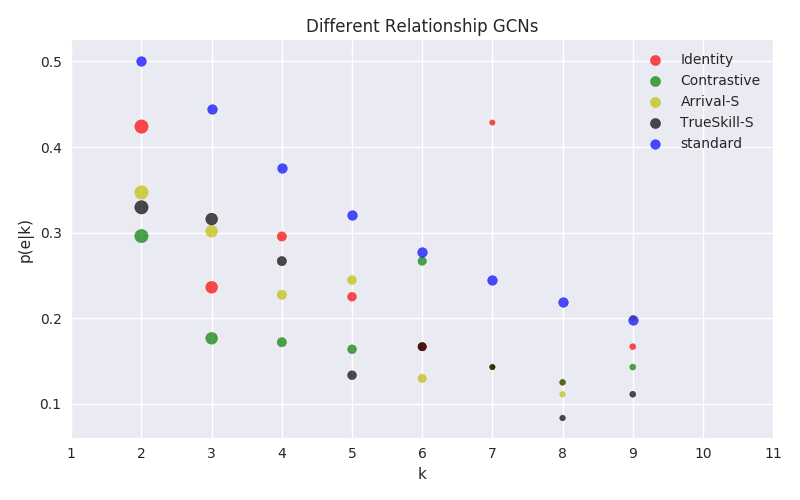
\includegraphics[scale=0.55]{figures/ErrorPlot.png}
  \caption{\label{fig:error} Probability of error with varying clique size for movie StackExchange. Standard represents random selection. Contrastive view outperforms other views for smaller clique sizes.  }
\end{figure}

Alternatively, we also plot the probability of error per tuple given each clique size ($p(e|k)$) for the movie StackExchange in \Cref{fig:error}. The \emph{standard} corresponds to a naive baseline of randomly selecting an accepted answer within each clique. For this standard baseline, error probability per clique can be denoted as,
\begin{align}
p(e|k) = (1 - 1/k) * \frac{2}{k} = \frac{2(k-1)}{k^2}
\end{align}
$(1 - 1/k)$ denotes the probability of choosing the wrong accepted answer, while $2/k$ is the actual error rate in these scenarios. The error rate is such because even in cases where the baseline chose the wrong accepted answer, remaining answers are still correctly classified as not accepted. Thus, there are only two errors per clique.

The standard baseline performs the worst as the error probability is highest than the other baselines for each clique. The Contrastive view has the least error probability for smaller cliques ($k<5$). This result is analogous to the performance gain illustrated above due to the \emph{Discriminative Magnification effect}. For larger cliques, similar contrast views (ArrivalSkill and TrueSkill) have the least error probability. As both of these views connects similar tuples across different questions, they are thus more useful for questions with a higher number of competing answers.



\subsection{Label Sparsity}

\begin{figure}[h]
      \centering
  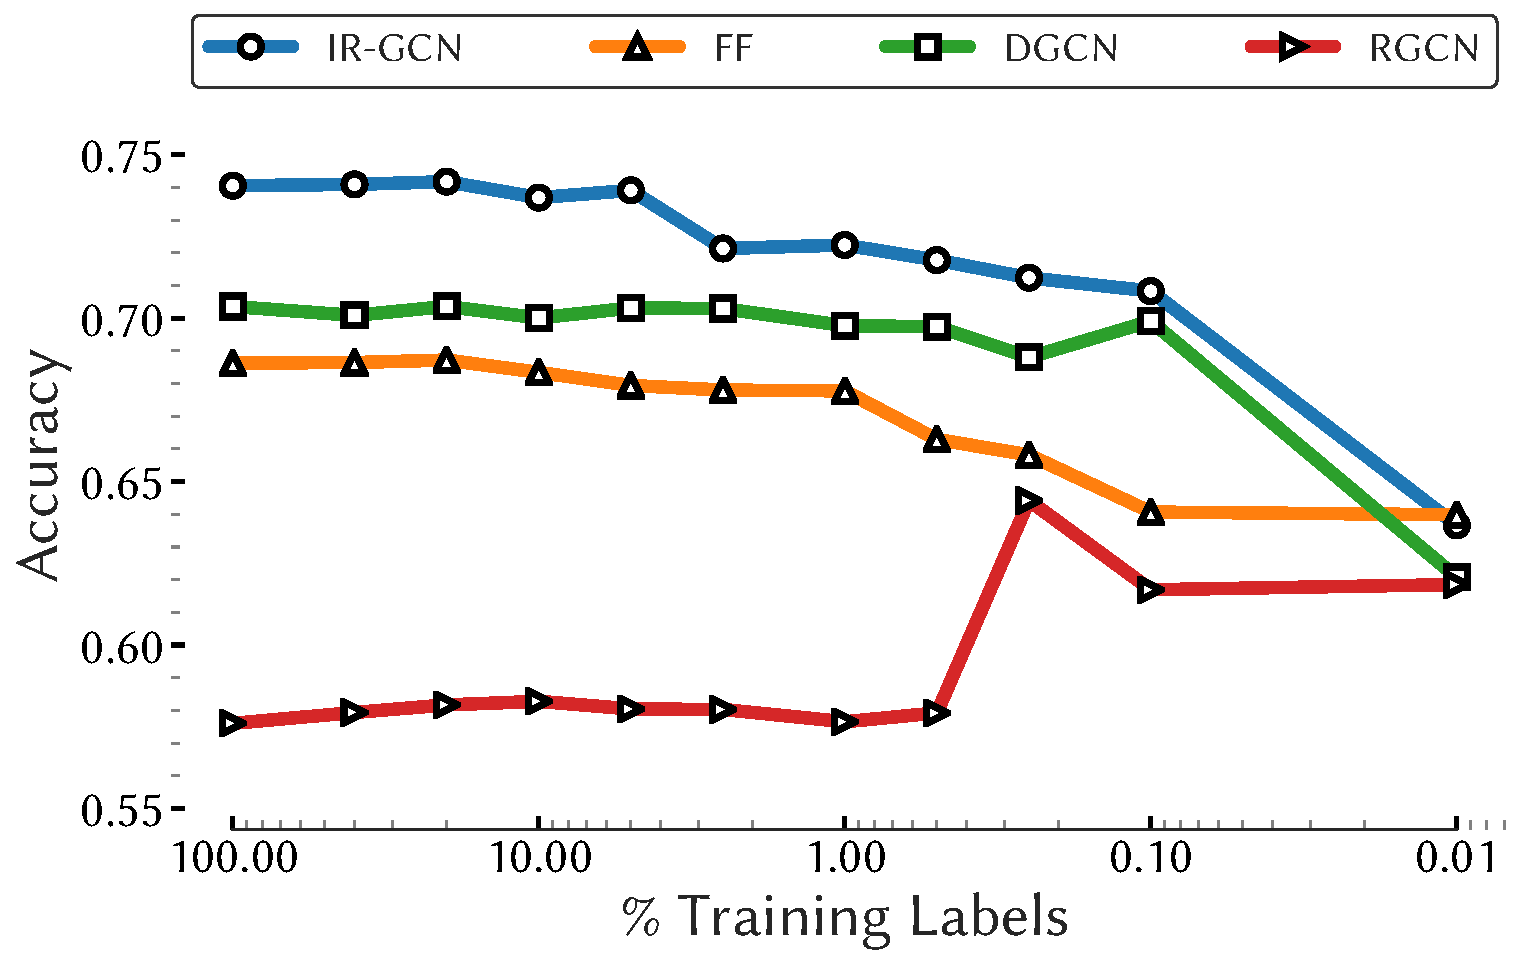
\includegraphics[scale=0.5]{figures/sparsity_acc_physics.pdf}
  \caption{\label{fig:labelsparsity} Change in accuracy with varying training label rates for Physics StackExchange. Our model is more robust to label sparsity than other relation ensemble approaches. RGCN works better with fewer labels as contrastive relation introduces noise in the model. At extreme sparsity, all approaches converge to the same value indicating random selection.}
\end{figure}
Graph Convolution Networks are robust to label sparsity as they exploit graph structure and are thus heavily used for semi-supervised settings. Figure \ref{fig:labelsparsity} shows the change in accuracy for Physics StackExchange from the Science category at different training label rates. Even though our graph contains disconnected cliques, IR-GCN still preserves robustness to label sparsity.
In contrast, the accuracy of the FeedForward model declines sharply with less label information. Performance of DualGCN remains relatively stable while Relational GCN's performance increases with a decrease in label rate. Relational GCN assumes each view to be of similarity relation, and thus, adding contrastive relation introduces noise in the model. However, as the training labels become extremely sparse, the training noise decreases that leads to a marked improvement in the model. In the case of an extremely low label rate of 0.01\%, all approaches converge to the same value, which is the expectation of theoretically random selection. We also obtained similar results for the other four StackExchange communities.


\subsection{Including Textual Features}
Most of the current literature focuses on using textual similarity for Answer Selection. In this section, we compare our proposed IR-GCN model to a popular text-based model~\cite{Tan2015} for answer selection.

\noindent
\textbf{Text Preprocessing}: For this experiment, we first preprocessed the text of both questions and answers.
We first removed all code snippets, HTML tags, stopwords, and URLs from the text of all questions and answers. We then tokenized the text using NLTK tokenizer followed by lemmatization using WordNetLemmatizer and finally converted it into lowercase.

We use torchtext (\url{https://pytorch.org/text/}) to create vocabulary and limit the text of each question and answer to be 250 words long. We initialized the words in the vocabulary using 300-dimensional pre-trained embeddings from Word2vec (\url{https://code.google.com/archive/p/word2vec/}). We randomly initialized words present in the vocabulary but not in word2vec.

We evaluate multiple approaches to test the effectiveness of incorporating textual features for answer selection task.
\noindent
\textbf{QA-LSTM/CNN \cite{Tan2015}} uses a stacked bidirectional LSTM model followed by convolution filters to extract embeddings for the question and answer text separately. Answers are then classified according to the cosine similarity of learned question and answer embedding.

Specifically, in this baseline, we use a biLSTM model with a hidden dimension = 300, followed by 50 1D convolutional filters with a kernel size of 3. We then compute the final embeddings by applying 1D max-pooling on the output of the convolution layer. We also used Tanh nonlinearity and a dropout of 0.3 on the final embeddings. We finally use these embeddings to compute a cosine similarity score between a question and its answers. This score is used to rank the candidate answers for evaluation. We implemented the baseline in Pytorch.

\noindent
\textbf{Textual Similarity (T-GCN)} We create a \textit{SimilarContrast} view that connects answers authored by a user where her answer is significantly similar (dissimilar) to the question than other competing answers. We used cosine similarity on the learned question and answer embedding from the QA-LSTM/CNN approach as the similarity function.

Specifically, we extract the updated embeddings of the question and answer text from the learnt QA-LSTM model. We then compute cosine similarity between the embeddings of each question and its answers.
We then connect answers authored by a specific user, where the difference in cosine similarity of the answer with the other competing answers is greater than margin $\lambda$. Specifically, if the user authors answers $a, a'$ to questions $q, q'$, we create a link between $a$ and $a'$ if
\begin{align}
 \lvert C_{q,a} - C_{q, b} \rvert &> \lambda; \forall b \in \mathcal{A}_(q) \\
 \lvert C_{q,a'} - C_{q, c} \rvert &> \lambda; \forall c \in \mathcal{A}_(q')
\end{align}
where $C_{q,a}$ is the cosine similarity of the answer $a$ with respect to question $q$. Similarly, a link is created for the opposite case when difference is less than $-\lambda$. In our experiments, we assign $\lambda = 0.4$. The hypothesis is that irrelevant(dissimilar) answers will more likely be rejected and vice versa.

\noindent
\textbf{IR-GCN + T-GCN} extends our proposed model to also include the Textual Similarity as the third \textit{SimilarContrast} view in addition to Arrival and TrueSkill Similarity.

\begin{table}[h]
  \centering
  \begin{tabular}{l | S[round-mode=places,round-precision=2]S[round-mode=places,round-precision=2]S[round-mode=places,round-precision=2]S[round-mode=places,round-precision=2]S[round-mode=places,round-precision=2]}
    \toprule
    {Method} &
      {Tech} &
      {Culture} &
      {Life} &
      {Sci} &
      {Business}\\
      \midrule
    QA-LSTM/CNN\cite{Tan2015} & 66.49 & 71.70  & 69.42 & 62.91 & 72.55 \\
    FF~\cite{JendersKN16} & 68.30 & 73.35 & 76.57 & 67.40 & 75.76 \\
    C-GCN & 71.23 & 75.90 & 78.71 & 72.99 & 76.85 \\
    T-GCN & 69.25 & 73.77 & 76.39 & 67.79 & 77.08\\
    IR-GCN & 73.87 & 78.74 & 81.60 & 74.68 & 80.56 \\
    IR-GCN + T-GCN & 73.89 & 78.00  & 81.07 & 74.49 & 78.86\\
    \bottomrule
  \end{tabular}
  \caption{\label{tab:text} 5-fold Accuracy comparison of text-based baseline and textual similarity GCN with IR-GCN.}
\end{table}

In general, the text-based baseline, QA-LSTM, performs worse than even reflexive GCN, as shown in Table \ref{tab:text}. Note that reflexive GCN employs a feedforward model on the activity and user features used in our experiments. This worse performance is surprising as most of the current literature focuses on textual features for the task. Our results indicate that non-textual features are useful too for answer selection task on StackExchange communities.

Textual Similarity GCN performs better than QA-LSTM and Reflexive GCN. Even though we use the output of QA-LSTM to construct the graph for T-GCN, the graph improves performance as it connects answers across questions. However, adding the T-GCN view in our proposed IR-GCN model decreases the performance slightly. One possible explanation could be that similar contrast views based on user features (Arrival similarity and TrueSkill similarity) are not compatible with views based on textual features.

\begin{table}[h]
  \centering
  \begin{tabular}{l | S[round-mode=places,round-precision=2]S[round-mode=places,round-precision=2]S[round-mode=places,round-precision=2]S[round-mode=places,round-precision=2]S[round-mode=places,round-precision=2]}
    \toprule
    {Method} &
      {Tech} &
      {Culture} &
      {Life} &
      {Sci} &
      {Business}\\
      \midrule
    QA-LSTM/CNN\cite{Tan2015} & 66.49 & 71.70 & 69.42 & 62.91 & 72.55 \\
    FF~\cite{JendersKN16} & 66.00 & 72.22 & 69.85 & 63.63 & 75.57 \\
    C-GCN & 66.19 & 72.45 & 70.23 & 63.89 & 75.71 \\
    CT-GCN & 66.06 & 72.35 & 71.88 & 64.14 & 75.69 \\
    IR-GCN & 66.56 & 72.92 & 72.54 & 65.11 & 75.95 \\
    IR-GCN + T-GCN & 66.49 & 73.17 & 72.85 & 65.29 & 75.86 \\
    \bottomrule
  \end{tabular}
  \caption{\label{tab:textfeature} 5-fold Accuracy comparison of text-based baseline and textual similarity GCN with learnt text embeddings as features in the GCN.}
\end{table}

We further replaced our activity-based features with the learned embeddings obtained after training the QA-LSTM/CNN~\cite{Tan2015} model as the node features. We observed that the performance of all approaches went down slightly when using textual features only (Table \ref{tab:textfeature}). As we noted before, GCNs aggregate features among the neighbors. In our similar contrast views, it is not favorable to aggregate textual features among the neighbors as it connects answers catering to different questions. Thus, aggregating textual features creates noise in the model leading to worse performance \footnote{We also experimented with concatenating textual features with the original features used in the previous experiments. However, the performance was still a little worse than the results with only original features.}.


\subsection{Contrastive GCN Analysis}
\label{ref:analysis}
The ability of neural networks to perform classification in sparse high-dimensional manifolds has been studied in past work, especially in the context of adversarial learning \cite{lu2017safetynet}. We employ the ReLU activation function in our convolution layers and study the outputs of the $k$th layer, i.e., embeddings with k-order locality. This transformation breaks the input space into cells with smooth gradients within each cell, at whose boundaries the piecewise linear function changes (i.e., the likelihood of the two classes of answers).

We ask a specific question in the context of our Contrastive GCN. \emph{What is the impact of the layerwise discriminative magnification induced by our formulation?} Discriminative magnifications result in improved separability of the two classes in the later convolving layers, an effect we earlier demonstrated with a sample network in \cref{fig:contrast}. This positively impacts the ability of the model to explain the observed data points (i.e., create p-domains that are well aligned with the contrastive samples provided) and improve the generalizability of the learned model to unseen data points. However, it is crucial to maintain sufficient regularization with weight decay to prevent sparse regions exhibiting sharp gradients that could affect model performance.

The capacity of our model can also be quantified in terms of the VC dimension of the aggregated classifier against the individual learners. Gradient boosting with multiple relation learners (each of which captures a specific aspect of node locality via graph convolution on the induced relations) could boost the capacity of the joint model, enabling better generalization and a more accurate fit in the data manifold (i.e., higher capacity to fit regions to fine distinctions).

Let us denote the upper bound of the VC dimension or capacity of each individual learner as D (If the individual learners do not have identical capacity, the minimum can be used to compute a lower bound on the aggregated learner capacity). Then the gradient boosted learner with T classifiers has a bound on it's capacity~\cite{shalev2014understanding} given by,
\begin{equation}
\mathcal{VC}_{Agg}  = T \times (D+1) \times(3 \log(T.(D+1))+2)
\label{vcdim}
\end{equation}

Thus we identify two potential reasons for our performance gains, first the discriminative magnification effect that also supports the strong individual performance of the contrast view, and second the gain in capacity from boosting, which could explain its advantage over competing aggregation methods.



\subsection{Limitations} We do recognize certain limitations of our work. First, we focus on equivalence relations that induce a graph comprising cliques. While cliques are useful graph objects for answer selection, equivalence relations may be too restrictive for other problems (e.g., the relation is not transitive). However, our modular framework does apply to arbitrary graphs, except that~\Cref{eq:restrictk} will no longer be an \emph{exact} convolution but be an approximation. Second, we assume no evolution in author skills. This assumption is not correct as users evolve with experience. We aim to address this in future work.

In summary, our model showed significant gains over state-of-the-art baselines for combining information from semantically different relational links in a graph. Our model is also more robust to training label sparsity as compared to other aggregator GCN approaches. We reasoned that the performance gains achieved by our aggregation strategy could be attributed in part to the enhanced learning capacity of the boosted model and the effect of discriminative feature magnification. We showed that content can also be used to induce graphs and performs better than using content features in isolation. Finally, we presented a few limitations and possible future extensions.

\section{Conclusion}
\label{sec:conclude}
This paper addressed the question of identifying the accepted answer to a question in CQA forums. We developed a novel induced relational graph convolutional (IR-GCN) framework to address this question. We made three contributions. First, we introduced a novel idea of using strategies to induce different views on $(q,a)$ tuples in CQA forums. Each view consists of cliques and encodes---reflexive, similar, contrastive---relation types. Second, we encoded label sharing and label contrast mechanisms within each clique through a GCN architecture.  Our novel contrastive architecture achieves \emph{Discriminative Magnification} between nodes. Finally, we show through extensive empirical results on StackExchange that boosting techniques improved learning in our convolutional model.
This was a surprising result since much of the work on neural architecture that are strong learners focuses on stacking, fusion or aggregator architectures. However, boosting is traditionally shown to be most effective with weak learners.
Our ablation studies show that the contrastive relation is most effective individually in StackExchange.


%\chapter{Joint Modeling of user latent behavior with semantic representation of text}
\chapter{Joint Modeling of user latent behavioral and content representations}
\label{chap:syntactic}
In this chapter, we jointly estimate user latent behavioral characteristics with improved text representations to improve offensive language prediction task.
Specifically, we estimate the abusive behavior of users, i.e., likelihood of posting an offensive content, on Twitter. Different from text representation approaches used in \Cref{chap:reliability} and \Cref{chap:induced}, we learn an improved text representation that is suitable to capture nuanced hate speech in text.
We further propagate user's abusive behavior through their social connections on Twitter to capture homophily in abusive user accounts. We finally show that combining the text and user representations can greatly improve offensive language prediction on future tweets \cite{hate}.

\section{Overview}
Abusive language usage in online social media is a grave issue that is affecting the interactions of users online. In a study conducted by Pew Research Center\footnote{http://www.pewinternet.org/2014/10/22/online-harassment/}, 40\% of adult Internet users have personally experienced harassment online, and 60\% have witnessed offensive name-calling. Social media websites, like Twitter and Facebook, allow users to report harassing content. However, due to the sheer volume of data, timely human curation of all reported content is not possible. Besides, there is also a need to filter these hateful content proactively. Therefore, there is an increased interest in automatic detection and moderation of hate speech in natural language processing \cite{waseem-hovy-2016}.

A typical definition of hate speech is as an \emph{attack} targeted towards a particular \emph{individual} or \emph{entity} belonging to
a protected group (protected group may include, but are not always limited to, religious, gender or racial minorities) \cite{elsherief2018hate}. Thus, hate speech identification can be cast as a relation extraction problem in which
the goal is to detect a "hate" or "attack" relation that links the speaker to a protected group (the object of the attack).

\begin{figure}[tbh]
    \centering
    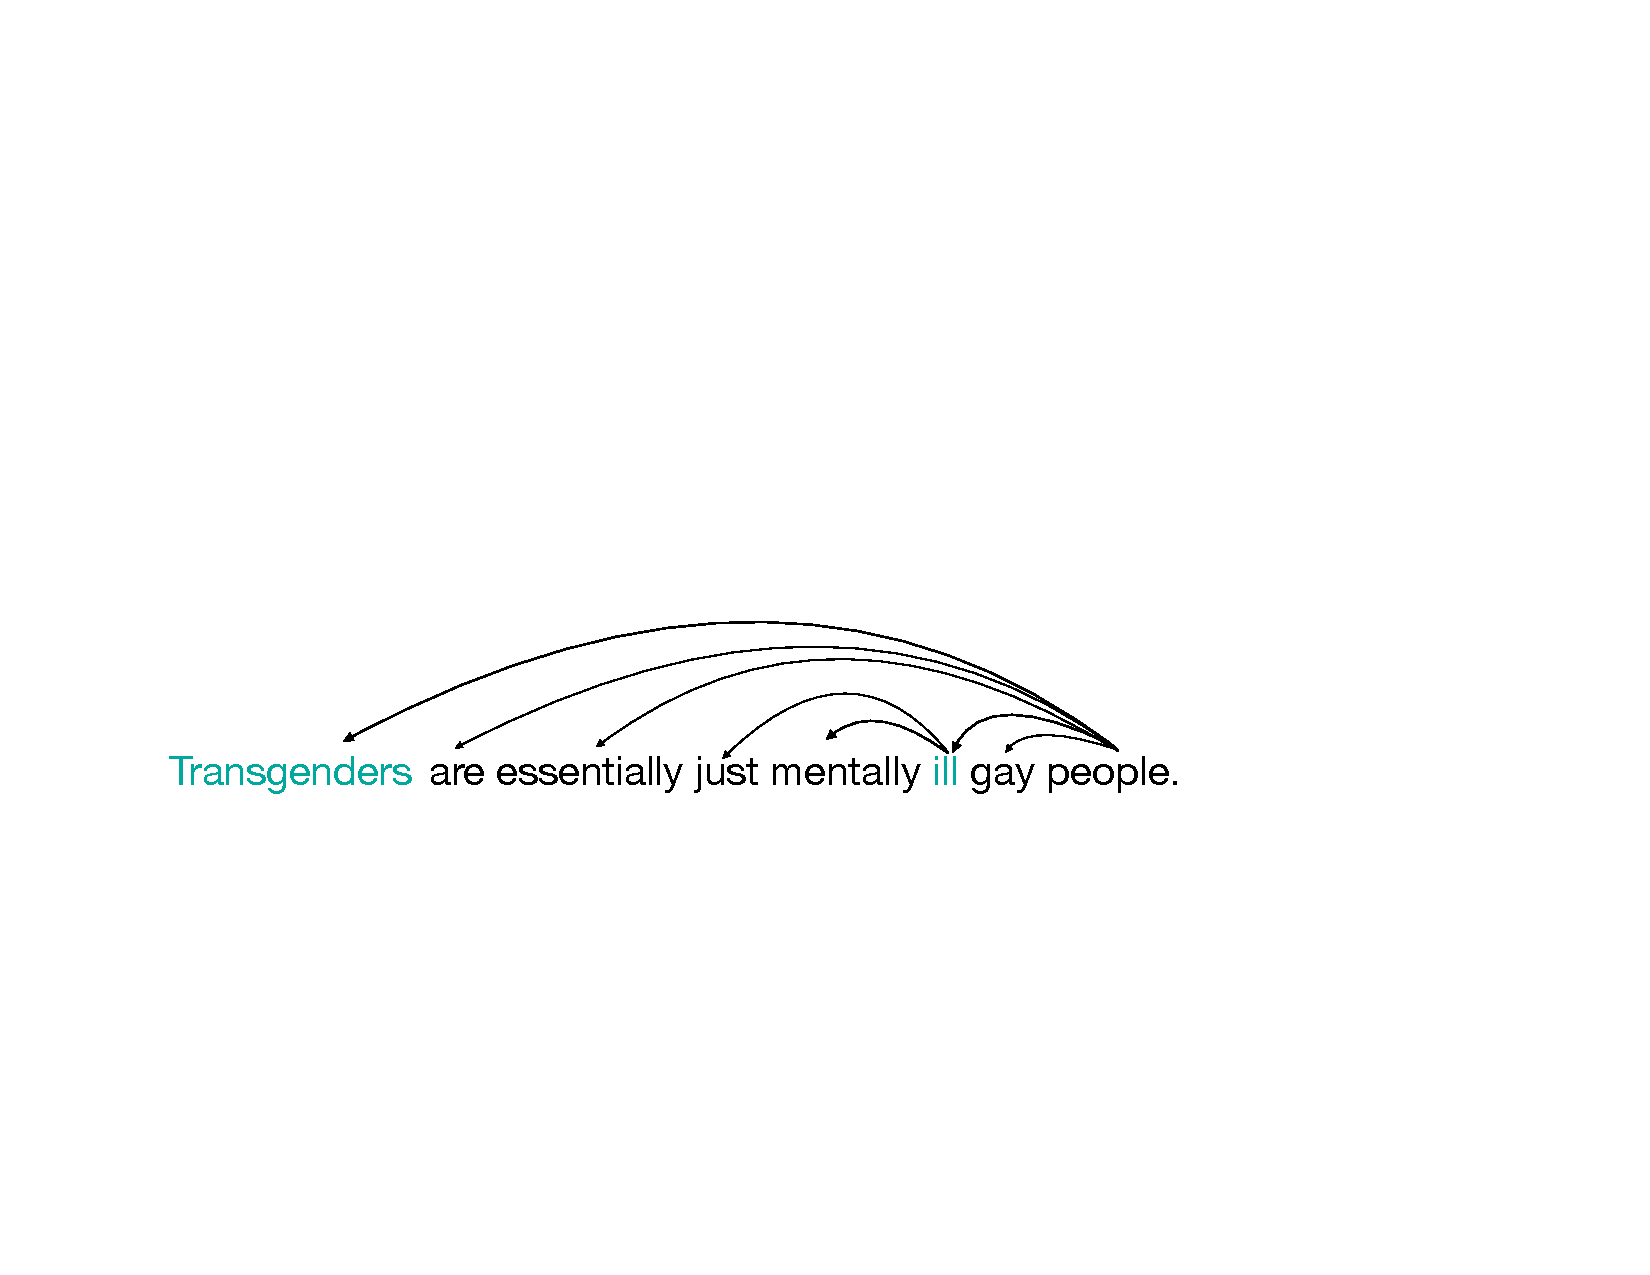
\includegraphics[scale=0.6]{figures/sample_key}
    \caption{Dependency parse for a sample hate tweet. The target \emph{Transgenders} is closer to the attack word, \emph{ill} in the parse tree. }
    \label{fig:parser}
\end{figure}


Current state-of-the-art methods in hate speech identification use either character or word n-gram features \cite{waseem-hovy-2016, davidson2017automated} or employ sequential deep learning models like CNN or LSTM \cite{ziqicnn, badjatiya2017deep}. However, these methods do not work well to capture long-range dependencies, for instance, in longer sentences with long clauses or complex scoping. Large pre-trained language models \cite{devlin2019bert} achieve very high accuracy after fine-tuning on supervised tasks. However, they typically learn pairwise attention between all words in the text and are thus computationally expensive. This makes them unfit to be used efficiently for real-time detection.

Recent work by \citet{clark2019does} analyzed attention mechanisms of the pre-trained BERT model and found that some of the attention heads are learning syntactic dependencies between words like direct objects of verbs, determiners of nouns, etc. A dependency parser also analyzes the grammatical structure of the sentence and returns the structure of syntactic dependence between words in the sentence. Recently, \citet{zhang-graph} used words in the dependency parse path between the subject and object of the sentence for extracting relations between them. They encoded the dependency parse graph using efficient graph convolution operations. Graph convolutional networks \cite{kipf2016semi} have been proposed for efficient convolutions over graph structured data. They are easy to parallelize and are computationally efficient.

However, a direct usage of \citet{zhang-graph}'s method is not straightforward because of the complexity of the possibilities for expressing the attack in text.
An attack may be expressed using explicit slurs or curses, as in: \emph{RT @USER: Stupid f*cking n*gger LeBron. You flipping jungle bunny monkey f*ggot}, or not, as in: \emph{Transgenders are essentially just mentally ill gay people}. In other instances, the attack can be \emph{implicit} like \emph{RT @USER: @USER every guy knows that the only thing that will make a woman happy is making any man a sandwich \#notsexist.}.
Moreover, the online text does not have annotated subject and object as in the benchmark datasets \cite{zhang-graph} and also often contains noisy text. However, parse structures can still be useful for capturing longer-range dependencies than sequential models (for instance, long clauses or complex scoping shown in these tweets). For instance, in Figure \ref{fig:parser}, the sequential distance between attack \emph{mentally ill} and target \emph{Transgenders} is five tokens, but while the distance in the parse tree is only two. Thus, we propose an adaption of the \cite{zhang-graph} model that learns a unified representation of text by encoding the whole dependency parse of the sentence. We later build a classifier based on this representation for identifying offensive language.

According to social influence theory \cite{social_influence}, users get influenced by their friends' behavior leading to user homophily \cite{homophily} (similar behavior) among connected users. Observable signals from social media can be taken as indicators of shared community membership.
\cite{mishra2019abusive} showed that most of the abusive behavior in their version of \citet{waseem-hovy-2016}'s dataset comes from a small set of densely connected users. They showed that incorporating user features along with linguistic features, can improve the hate classification task. We propose an extended version of our model that uses a user social graph in addition to the parser graph to learn extended embeddings.

%//Talk about our contributions and methods
In this work, we propose a classifier based on dependency graphical convolutional networks (DepGCN) to detect offensive language online. We tested our method on the benchmark Twitter hate speech datasets. Our model outperformed the current state-of-the-art \cite{waseem-hovy-2016, davidson2017automated} for offensive language detection and even strong baselines like fine-tuned BERT \cite{devlin2019bert}. We further propose a UserGCN model to incorporate the effect of social influence on user's abusive behavior. The UserGCN model learns a user's abusive behavior through a class prior and propagates this behavior through their social network. After merging the DepGCN with the UserGCN model, we achieve a new state-of-the-art on these benchmark datasets.

\section{Proposed Method}
In this section, we first describe how we represent text as a graph using the dependency parse tree. We then convolve over this dependency graph using a graph convolutional framework (DepGCN) to compute a text embedding used for offensive language detection task. Further, we describe our novel GCN based architecture that exploits the user social graph to augment the text embeddings.

\subsection{Graph representation of Text}
We use the dependency parse tree to induce a graph on a sentence. Specifically, a graph $G = < V, E > $ is represented as a collection of vertices $V$ and as a set of edges $E$ between these vertices. Thus, to compute the graphical representation of the sentence, we treat each word as a vertex, with syntactic dependencies between words corresponding to an edge. Now, for this graph $G$, $\textbf{A}$ represents the Adjacency matrix where $A_{ij} = 1$ if there is a dependency relation between word $i$ and $j$ and $0$ otherwise. We also connect each word to itself such that $A_{i,i}$ = 1; $\forall i \in V$. Although syntactic dependencies are directed, we treat these dependency edges as undirected, resulting in a symmetric matrix\footnote{Similar to \cite{zhang-graph}, we observed a performance dip when using each edge direction as a separate graph.}.

Graph Convolution Networks (GCN) are recently proposed to compute vertex embeddings in a graph by convolving over each vertex's local neighborhood \cite{kipf2016semi}.

The convolution operation for vertex $i$ in layer $k$ in GCN is defined as follows,

\begin{align}
    h_i^{k+1} &= \sigma \left ( \sum_{j = 1}^{|V|}  \tilde{A}_{ij} W^k h_j^k + b^k  \right ) \\
    &= \sigma \left ( \frac{ \sum\limits_{j \in \mathcal{N}(i) \cup i} W^k h_j^k} {d_i} + b^k  \right )
\end{align}
where $\mathbf{\tilde{A}} = D^{-1/2}\mathbf{A}D^{1/2}$ is the normalized Adjacency matrix with $D$ being the degree matrix. $h_i^{k+1}$ represents the vertex embeddings at layer $k+1$, with $h_i^0$ being initialized with the vertex features. In our case, we use pretrained word embeddings as the initial features.
$W^k, b^k$ are learnable weight and bias parameters of layer $k$ and $\sigma$ represents the ReLU function. $\mathcal{N}(i)$ represents the vertex \emph{i}'s neighborhood while $d_i = \sum {D}_i$ represents the vertex degree.

Now, assume that $W^k = \mathbf{{I}}$ with $b^k = 0$ and $\sigma(.)$ as an identity function. The updated vertex embedding at layer $k+1$ will be,
\begin{align}
    h_i^{k+1} &= \frac{ \sum\limits_{j \in \mathcal{N}(i) \cup i} h_j^k} {d_i}
\end{align}
It is thus easy to verify that the convolution operation updates the vertex embeddings at layer $k+1$ to be the average embeddings of the vertex's neighborhood and the vertex itself from the previous layer, $k$. In our dependency graph, applying graph convolution operation will augment each word's embedding with its syntactic neighbors.
Thus, convolution helps to contextualize the word embeddings, where the word's syntactic relationships define the context. Notice that it is different from the sequential models (like LSTM or CNN), where the adjacent words in the sentence define the context.

Consider the sample tweet in Figure \ref{fig:parser}, first, \textit{ill} will be augmented with its surrounding adverbs \textit{mentally} and \textit{just} (\cref{eq:sample}). In turn, these updated embeddings of \textit{ill} will be propagated when computing embeddings of the noun \textit{people} in addition to the subject \textit{Transgenders}.
\begin{align}
      \label{eq:sample}
      h_{ill} &= f_{gcn}(h_{mentally}, h_{just}, h_{ill}) \\
      h_{people} &= f_{gcn}(h_{ill}, h_{transgenders}, h_{people})
\end{align}
However, in sequential models with a fixed window, the attack \textit{ill} will be too far from the subject \textit{Transgenders}.

Further, by stacking such $k$ convolution layers, we can propagate the vertex embeddings to its k-hop neighborhood \cite{kipf2016semi}. For our experiments, we did not see any further improvements after two layers. This could be because, as we are dealing with a short text, the resulting parse tree is shallow.

\subsection{Sentence representation}
In the previous section, we computed contextualized word embeddings using syntactic relationships. However, we still need to aggregate these node embeddings to compute a graph-level embedding (sentence in our case). In particular, we perform masked pooling over the learned word embeddings from the last layer ($K$) to compute a sentence embedding. We only pooled over non-terminal words or intermediary nodes in the dependency parse tree (i.e. $\vert A_{i} \vert > 2$). We ignored the leaf words or words linked to only one other word as their word embeddings are relatively unchanged (because of less number of neighbors) after the convolution as compared to other intermediary nodes with more neighbors. Thus, when we perform pooling over all the words, leaf words will skew the final result even though they are not always important. We tried different variants of pooling (average and min), but max-pooling performed the best (\cref{eq:max}) for our case.
\begin{align}
  \label{eq:max}
    h_G &= \max_{i \in V'} (h_i^K) \; s.t. \vert A_{i} \vert = 2
\end{align}
Further, these sentence embeddings are fed through fully connected layers followed by a sigmoid ($\sigma$) to compute final class score (\cref{eq:class}) for the sentence.
\begin{equation}
    c_G =   \sigma (f_{MLP}(h_G)); c_G \in \mathbf{R}^C
    \label{eq:class}
\end{equation}
Here, $C$ represents the total number of classes.

\subsection{Embedding variants}
As we deal with noisy text, there can be ill-formed words and grammatically incorrect sentences that can lead to incorrect parse trees. Thus, to overcome these potential errors, we feed the initial word embeddings ($h_i^0$) to a BiLSTM module. The BiLSTM module helps to aid in word disambiguation by encoding adjacent words in the sentence.

\begin{figure}
    \centering
    \includegraphics[scale=0.6]{figures/architecture_key.pdf}
    \caption{Overview of our proposed model}
    \label{fig:arch}
\end{figure}
The final architecture of our dependency graph convolution network (DepGCN) is depicted in \Cref{fig:arch}.
\subsection{User Features}
\citet{mishra2019abusive} observed that only a small set of users were responsible for most of the offensive tweets in the \citet{waseem-hovy-2016} dataset. In a similar analysis on tweets posted in response to President Obama's re-election, \citet{racist_article} found that most of the racist tweets came from only a group of states. Thus, it shows that determining the author of the tweet will be beneficial for automated offensive language detection.

Further, prior studies have shown that user behavior is influenced by their friends in online social networks leading to similar behavior(user homophily) of connected users \cite{homophily, social_influence}.
To empirically verify this in \citet{waseem-hovy-2016} dataset, we computed the average cosine similarity between the class distribution of a user's tweets and their friends' tweets. We observed a high similarity value of \emph{0.80}, indicating similar tweeting behavior between connected users. In other words, this high value shows that users connected to offensive users tend to follow suit. Thus, modeling the influence of user's social connections can potentially improve our understanding of user behavior.
We thus extend our proposed model to augment the sentence embeddings obtained from DepGCN with the social embeddings capturing user and her friends' tweeting behavior.

To this end, we use the follower followee relationship of each user in our dataset from Twitter\footnote{Thanks to authors of \cite{mishra2019abusive} for providing the user social relationship data.}. Similar to the dependency graph, we create a social graph and represent each user as a vertex, and the edges represent the follower relationship. For our experiments, we treat the follower-followee relationship as equivalent. We believe that it is a reasonable assumption, as in general, follower-followee relationships are often reciprocal, and our dataset does not contain any celebrities (skewed ratio of followers vs. followee).

To capture the user's tweeting behavior, we first compute user embeddings ($e_u$) as the average of the sentence embeddings obtained from DepGCN, for all the tweets authored by the user (\cref{eq:user}).
\begin{align}
\label{eq:user}
    e_u &= \frac {\sum_T h_T} {\vert \mathcal{A}(u) \vert}; \forall T \in \mathcal{A}(u)
\end{align}
$\mathcal{A}(u)$ represents all the tweets authored by the user $u$.

To capture the effect of homophily, we perform graph convolution operation on the user's social graph with these user embeddings being used as initial vertex features ($h_u^0$).

In the first layer of the graph convolution, we project these user embeddings to a $C$ dimensional vector to learn the user's prior distribution per class. It is not correct to classify each user or all her tweets to be abusive or not. Therefore, we learn a class probability for each user, which indicates her likelihood of posting an offensive tweet.

In the subsequent layers, we propagate these class priors through the user's social network.
\begin{equation}
    h_u^k = \sigma \left ( \frac{ \sum_{v \in \mathcal{N}(u) \cup u} W^k h_v^k} {d_u} + b^k  \right )
\end{equation}
where $\mathcal{N}(u)$ denotes the friends of user $u$.

\begin{align}
    h_S &= \sigma (h_u^K) \\
    c_F &= f_{MLP}( [h_G, h_S] )
\end{align}
where $h_S \in R^C$ are social embeddings for user who tweeted the tweet.
Finally, we concatenate the text and social embeddings for each tweet and compute the final class probability.
The final architecture of UserGCN with our DepGCN is depicted in \Cref{fig:userarch}.

\begin{figure}
    \centering
    \includegraphics[scale=0.6]{figures/Userarchitecture_key}
    \caption{Overview of our proposed model with user social graph}
    \label{fig:userarch}
\end{figure}

\section{Experiments}
In this section, we first describe our experimental setup, followed by the performance results. We then present a detailed error analysis of our dependency-based model vs. a widely-used sequential model for sentence classification. Finally, we present results for an approach that augments the textual embeddings with the user's social information.

\subsection{Experimental Setup}
We first describe our datasets, followed by comparative baselines.

\noindent
\textbf{Datasets:}
\citet{wiegand-etal-2019-detection} emphasizes the difficulty of selecting representative datasets for studying abusive language. At the heart of this difficulty is the relative rarity of hate speech in the large-scale user-generated text. It is not unusual for $> 99\%$ of text to be benign.

To make experiments manageable \citet{waseem-hovy-2016}
bootstrap data collection with queries that are indicators of possible hate speech. As a result of this bootstrapping, the data collected is {\em not} representative of the underlying text distribution. This {\em data bias} applies to both the benign and the offensive categories.

\citet{davidson2017automated} provides an alternative dataset, but this, too, is affected by pre-filtering, with the result that the dataset also fails to represent the underlying text distribution. Thus, caution is advised when interpreting the results of studies on these datasets. \citet{wiegand-etal-2019-detection} suggests several mitigations for the deficiencies of these datasets, as well as cross-classification methods that can sometimes diagnose over-optimism about classification results.

For comparability, we experiment with both the datasets from \citet{davidson2017automated} and \citet{waseem-hovy-2016}.
We do not claim that our results will necessarily transfer to more naturalistic settings. \Cref{tab:data} lists the per class distribution in the collected dataset. Note that as previously noted, \citet{davidson2017automated} dataset is highly skewed, with the majority of tweets being offensive. We thus also create a custom dataset (Davidson ext.) to mimic the real-world settings, by adding benign tweets from \citet{waseem-hovy-2016} to \citet{davidson2017automated}'s benign tweets.

\begin{table*}[h]
  \centering
  \small
\begin{tabular}{ l c c  c }
\toprule
 Dataset &  \multicolumn{3}{c}{{Categories}} \\
  \midrule
 \multirow{2}{*}{\citet{davidson2017automated}}& Hate & Offensive & Benign \\ \cline{2-4}
              & 1,430 & 19,190 & 4,163 \\
 \multirow{2}{*}{\citet{waseem-hovy-2016}}& Racism & Sexism & Benign \\ \cline{2-4}
 & 1,939 & 3,148 & 11,115 \\
 Davidson extended   &  Hate & Offensive & Benign \\ \cline{2-4}
 & 1,430 & 19,190 & 15,278 \\
 \bottomrule %\hline
\end{tabular}
\caption{\label{tab:data} Dataset Statistics. }
\end{table*}

\textbf{Baselines:}
We compare against a variety of state-of-the-art approaches proposed for computing sentence embeddings. We use these embeddings to classify the tweets into offensive or not.
\begin{itemize}
\item \textbf{N-grams} Current state-of-the-art approach for hate speech classification \cite{waseem-hovy-2016} extracts N-grams of the tweets and feed them into logistic regression along with Twitter-specific features per tweet.
%\item \textbf{Tf-Idf} approach extracts tf-idf features of each tweet which are then fed into linear SVM for classification \cite{davidson2017automated}.
\item \textbf{BERT} BERT, \citet{devlin2019bert} provides a variety of text embeddings, which have achieved new state-of-the-art results on multiple natural language tasks such as question answering and language inference. For our experiments, we initially fine-tune the $BERT_{base}$ model on our training dataset. We then extract the embeddings of each tweet from the trained model and feed them to a feedforward network to compute the final class score.

\item \textbf{BiLSTM} is a
% popular -- doesn't matter whether it is popular
sequential model to compute sentence embeddings that is useful for many downstream classification tasks \cite{bilstm}. We use the output of the final hidden layer in the BiLSTM as the sentence embeddings.
We follow BERT in feeding the sentence embeddings to a feed-forward network to compute the final class-wise score.
\end{itemize}

\noindent
\textbf{Implementation Details:}
We initialize $h_i^0$ of each word with its Glove embeddings \cite{glove} combined with its POS tag, NER tag, and dependency relation given by the Stanford NLP API. We use the Stanford parser\footnote{\url{https://nlp.stanford.edu/software/lex-parser.shtml}} for extracting the dependency parse relationship between the words in a tweet. We perform stratified sampling on the dataset to create an 80-10-10 split
between training, development and test sets. The development set is used for hyperparameter tuning while the results are reported on the test set. We report the class-wise F1 score for each dataset. We implement our model and the baselines in PyTorch and run the experiments on an Nvidia Tesla V100 GPU. We use a two-layer GCN for both DepGCN and UserGCN. We use a \emph{weighted} cross-entropy loss to counter the effect of class imbalance.
We do for all the baselines and our proposed approach.

%\noindent
\subsection{Performance Analysis:}

Table \ref{tab:davidsonext} reports class-wise F1 score with weighted F1 for the \citet{davidson2017automated} extended dataset. As expected, the bag-of-words based N-gram approach
is not competitive with the best approaches. This is reasonable, since that approach
does not take any advantage of semantic similarities between different words.
% performs the worst out of all the approaches as they do no leverage the semantic meaning of the words.
More surprisingly, the state-of-the-art BERT model, even after fine-tuning, still performs slightly worse than our DepGCN model.

\begin{table}[tbh]
  \centering
  \small
  %\setlength{\tabcolsep}{2pt}
\begin{tabular}{ l | c c  c c }
\toprule %\hline
 Approach &  Hate & Offensive & Benign & Overall \\ %\hline
  \midrule
 N-grams & 0.35 & 0.88 & 0.88 & 0.85\\
 %Tf-Idf & 0.45 & 0.94 & 0.96 \\
 BERT & 0.45 & 0.94 & 0.96 & 0.91\\
 %Emb + Pooling & 0.35 & 0.88 & 0.88 \\
 BiLSTM & 0.31 & 0.93 & 0.94 & 0.90\\
 DepGCN & 0.47 & 0.94 & 0.96 & 0.92\\
 BiLSTM + DepGCN & \textbf{0.49} & \textbf{0.95} & \textbf{0.97} & \textbf{0.93}\\
 \bottomrule %\hline
\end{tabular}
\caption{\label{tab:davidsonext} Class-wise F1 score with the overall weighted F1 score for different approaches on the \citet{davidson2017automated} extended dataset.}
\end{table}

The sequential model, i.e., BiLSTM, also performs worse than our dependency-based model. As argued before, sequential models often struggle to capture long term dependencies between words while DepGCN alleviates this issue by encoding syntactic dependencies. Further, if we use BiLSTM to contextualize the embeddings before feeding it to our DepGCN model, the results are slightly improved. Note that even a slight improvement in the hate class is significant as the dataset contains limited training examples for this class (\Cref{tab:data}) as compared to the other classes.

\begin{table}[tbh]
  \centering
  \small
  \setlength{\tabcolsep}{2pt}
\begin{tabular}{ l | c c  c c}
\toprule %\hline
 Approach &  Hate & Offensive & Benign & Overall \\ %\hline
  \midrule
 N-grams & 0.46 & 0.94 & 0.84 & 0.89 \\
 BERT & 0.42 & \textbf{0.95} & \textbf{0.88} & \textbf{0.91} \\
 %Emb + Pooling & 0.35 & 0.88 & 0.88 \\
BiLSTM & 0.52 & 0.94 & 0.86 & 0.90 \\
DepGCN & 0.50 & 0.94 & 0.86 & 0.90 \\
BiLSTM + DepGCN & \textbf{0.53} & 0.94 & 0.87 & \textbf{0.91} \\
 \bottomrule %\hline
\end{tabular}
\caption{\label{tab:davidson} Class-wise F1 score with the overall weighted F1 score for different approaches on the \citet{davidson2017automated} dataset.}
\end{table}

We obtain a similar trend in the results when evaluating performance on the original \citet{davidson2017automated} dataset, as shown in Table \ref{tab:davidson}. BERT becomes more competitive on the original dataset. The Benign class of the original dataset has systematically lower figures than the corresponding class in the extended dataset, presumably because the extended data set has a better representation of the space of possible benign examples. The Hate class is slightly easier to detect in the original dataset, even though it contains the same examples as the corresponding class in the extended dataset, presumably because the classifiers expend more of their modeling capacity on the benign set. The same pattern is present to a lesser degree for the Offensive class.
BERT becomes more competitive with BiLSTM on the original dataset. BiLSTM retains a substantial ($0.53 > 0.48$) advantage over BERT on the Hate class, and is close on Offensive and Benign.

The sequential model, BiLSTM, performs slightly better than our DepGCN model. One possible explanation can be that the \citet{davidson2017automated} dataset is full of \emph{slurs} and \emph{direct} hate attacks on entities. These \emph{direct} attacks do not exhibit long-range dependencies and thus, are well captured by the sequential models. Also, due to the heavy usage of \emph{slurs}, BERT performs worse as there are many OOV tokens in the dataset.

\begin{table}[tbh]
  \centering
  \small
  \setlength{\tabcolsep}{2pt}
\begin{tabular}{ l | c c  c c}
\toprule %\hline
 Approach &  Racist & Sexist & Benign & Overall \\ %\hline
  \midrule
 N-grams & 0.75 & 0.71 & 0.88 & 0.83 \\
 BERT & 0.78 & \textbf{0.81} & \textbf{0.91} & \textbf{0.88} \\
 %Emb + Pooling & 0.35 & 0.88 & 0.88 \\
BiLSTM & 0.72 & 0.71 & 0.89 & 0.84 \\
DepGCN & 0.76 & 0.72 & 0.88 & 0.83 \\
BiLSTM + DepGCN & \textbf{0.78} & 0.74 & 0.90 & 0.85 \\
 \bottomrule %\hline
\end{tabular}
\caption{\label{tab:waseem} Class-wise F1 score with the overall weighted F1 score for different approaches on the \citet{waseem-hovy-2016} dataset.}
\end{table}

On a more nuanced dataset collected by \citet{waseem-hovy-2016}, BERT performs the best out of the competing methods, as shown in \Cref{tab:waseem}. Our model performs competitively for racist and benign tweets while it performs worse for sexist tweets. This dataset is more nuanced as it contains more indirect or implied hate attacks (discussed in \cref{sec:error}) with the usage of fewer slurs. Thus, the powerful language model BERT can better capture the meanings of these tweets.

\begin{figure}[tbh]
\centering
\begin{subfigure}{0.45\textwidth}
%\centering
  \includegraphics[scale=0.37]{figures/Traintime}
  \caption{Inference time}
  \label{fig:test}
  \end{subfigure}\hfill{}
  \begin{subfigure}{0.45\textwidth}
  %\centering
    \includegraphics[scale=0.37]{figures/Testtime}
    \caption{Training time}
    \label{fig:train}
    \end{subfigure}
    \caption{\label{fig:time} Time analysis of variants of our model with respect to the popular BERT \cite{devlin2019bert} language model. }
\end{figure}

\noindent
\textbf{Time Analysis :} We further compare the running time analysis of all the baseline approaches. \Cref{fig:time} shows the comparison for both training time and inference time. First, in \Cref{fig:test}, we plot the inference time (in secs) required by each approach per 1000 tweets. Our proposed DepGCN is the most efficient approach at inference time closely followed by BiLSTM. Adding the BiLSTM module before the DepGCN only increases the inference time slightly. However, BERT, on the other hand, takes an order of magnitude longer than any of these approaches. Note that the inference time does not take into account the time taken to extract the parse tree for the tweets. However, as we are looking at a short text, this time is negligible.
The same trend can be observed for training time too in \Cref{fig:train}. However, the jump from DepGCN to BiLSTM training time is a little higher than during inference.

Thus, our parser-based DepGCN approach is much more efficient than the BERT model. Also, including BiLSTM module to the DepGCN model leads to only a slight drop in efficiency.


\subsection{Error Analysis of Sequential vs. Dependency model}
\label{sec:error}
In this section, we present a detailed analysis of the errors of the sequential (BiLSTM) vs. Dependency (DepGCN) model. Table \ref{tab:confusion} shows the confusion matrix of BiLSTM vs DepGCN model on the Waseem dataset. The parser-based approach is more conservative in labeling tweets as benign than the sequential approach. Specifically, sexist tweets are more probable to be misclassified as racist and vice versa.
Alternatively, DepGCN tags much more benign tweets as offensive (Sexist/Racist), thus creating more false positives. However, as there is a higher cost involved in missing an offensive tweet, DepGCNs will be more effective in real-world scenarios.

%\textbf{Sequential vs. Dependency based models:}

\begin{table}[tbh]
  \small
  %\setlength{\tabcolsep}{1pt}
  \begin{subtable}{0.5\linewidth}
    \centering
\begin{tabular}{ l  r  r r }
\toprule %\hline
  &  Racism & Sexism & Benign  \\ %\cmidrule(lr){2-7}
  %\hline
  \midrule
 Racism & 7 & 11 & 7 \\
 Sexism & 7 & 11 & 8 \\
 Benign & 35 & 70 & 33 \\
 \bottomrule %\hline
\end{tabular}
\caption{Dependency Parser model}
\end{subtable}%
\begin{subtable}{0.5\linewidth}
  \centering
\begin{tabular}{ l  r  r r }
\toprule %\hline
&  Racism & Sexism & Benign  \\
\midrule
Racism & 4 & 3 & 18 \\
Sexism & 1 & 7 & 18 \\
Benign & 9 & 25 & 104 \\
\bottomrule %\hline
\end{tabular}
\caption{Sequential Model}
\end{subtable}
\caption{\label{tab:confusion} Confusion matrix for Sequential (BiLSTM only) vs Dependency Parser (GCN only) approach for \citet{waseem-hovy-2016} dataset.}
\end{table}

We also examined some sample tweets from the \citet{waseem-hovy-2016} dataset, which were erroneously classified as benign by BiLSTM but not by DepGCN and vice versa to understand the difference between these two approaches in depth.

\begin{figure*}[tbh]
  \begin{subfigure}{\textwidth}
  \centering
  \includegraphics[scale=0.65]{figures/Example1_key}
  \caption{Parse tree of the sexist tweet missed by LSTM.}
  \label{fig:sample}
  \end{subfigure}

  \begin{subfigure}{\textwidth}
    \centering
    \includegraphics[scale=0.6]{figures/example2_key}
    \caption{Parse tree of the sexist tweet missed by DepGCN}
    \label{fig:example}
  \end{subfigure}

  \begin{subfigure}{\textwidth}
  \centering
    \includegraphics[scale=0.65]{figures/example3_key}
    \label{fig:example3}\caption{Parse tree of the racist tweet missed by DepGCN.}
    \end{subfigure}
    \begin{subfigure}{\textwidth}
    \centering
      \includegraphics[scale=0.65]{figures/example3_2_key}
      \label{fig:examplecoref}\caption{Coreference resolution of the tweet.}
      \end{subfigure}

  \label{fig:examples}
  \caption{Parse Tree of the two sample tweets from Waseem dataset.}
\end{figure*}

\emph{Sexist tweet missed by LSTM}: Following is a sample sexist tweet that is correctly classified by the DepGCN approach but missed by the BiLSTM.
\textit{"I'm not sexist but women get upset with other women for stupid reasons. Women constantly say they have "haters"."}
\Cref{fig:sample} shows the parse tree of the tweet by the Stanford parser. It is a difficult sample to classify as the author of the tweet says that he is \textit{not} sexist but is writing offensive remarks against women. The dependency tree can capture this long-range dependency and establish negative relation of "upset," "stupid," and "haters" with the "women" subject.


\emph{Sexist tweet missed by DepGCN}: However, DepGCN fails to capture similar nuanced sexism in another sample tweet, \textit{"And when they're all PMSing at the same time LOL I'm not sexist, but I can't work with 5 female managers at the same time anymore.""}. Note that the sentence contains punctuation error as it is missing punctuation between the two sentences in the tweet (after \textit{time} and before \textit{I'm not}). This error leads to a wrong parse tree, as shown in \Cref{fig:example}. Thus, our parser-based model is sensitive to these parsing errors.

\emph{Racist tweet missed by DepGCN}: However, even if the parse tree is correct, just establishing dependency relationships may not be sufficient to capture nuanced relationships in the text. For instance, the parse tree of the racist tweet,
\textit{"Here is the Quran telling Muslim men that they can rape their slave girls."} shown in \Cref{fig:example3} is correct. However, the parse tree misses the coreference of pronouns \textit{they} and \textit{their} to belong to \textit{Muslim men}. In these cases, powerful language models like BERT will be able to extract these relationships.

\subsection{Effect of User Social Graph}
\Cref{tab:waseemuser} shows the class-wise F1 scores after adding the user social graph with the DepGCN model on the \citet{waseem-hovy-2016} dataset. We do not report results on the other datasets as we have do not have any information about their users. UserGCN used in isolation performs worse than the other approaches.
This poor performance is expected as it ignores the textual information entirely. Note that the UserGCN uses the user's class prior only for prediction for all of the user's tweets. However, even with that naive methodology, this model achieves similar performance to the previous state-of-the-art linguistic approach, N-gram (\Cref{tab:waseem}), and our DepGCN model for the sexist class.

\begin{table}[tbh]
  \centering
  \small
  \setlength{\tabcolsep}{2pt}
\begin{tabular}{ p{35mm} | c c  c c}
\toprule
 Approach &  Racist & Sexist & Clean & Overall \\
  \midrule
 BERT & 0.78 & 0.81 & 0.91 & 0.88 \\
 BiLSTM + DepGCN & \textbf{0.78} & 0.74 & 0.90 & 0.85 \\
 UserGCN & 0.61 & 0.72 & 0.79 & 0.74 \\
 BiLSTM+DepGCN \\ +UserGCN & \textbf{0.79} & \textbf{0.82} & \textbf{0.92} & \textbf{0.88} \\

 \bottomrule
\end{tabular}
\caption{\label{tab:waseemuser} Comparison of class-wise F1 score with weighted F1 score for different approaches with our proposed approach after adding the user social features on \citet{waseem-hovy-2016} dataset.}
\end{table}

After adding the user features, our model improves by 0.03 F1 points and slightly outperforms the previously best performing BERT model. The most significant improvement comes from the tweets annotated as sexist (similar trend seen in UserGCN). This improvement indicates that there is a strong homophily effect in users authoring sexist tweets in the dataset. As noted by \citet{mishra2019abusive}, racist tweets in this dataset are contributed by only five users who also tweet other benign and sexist tweets. Thus, incorporating additional user information does not give us higher gains for the racist class.

\section{Conclusion}
In this work, we propose a sentence encoder that extends the graph convolutional network (GCN) to an induced graph built from syntactic dependencies in the text for offensive language detection.
Our model achieved state-of-the-art performance on public hate speech twitter datasets without the use of user features. The overall performance matches or exceeds that of strong baselines such as fine-tuned BERT.
Our framework is interpretable and allows efficient parallel batch processing. Finally, we show that addition of user features is able to gain benefit from strong user homophily in the abusive user accounts that we worked with. This is achieved using a network architecture that allows behavioral priors to propagate from user to user.


\chapter{Conclusion}
\label{chap:concl}
In this chapter, we summarize the contributions of this dissertation and then discuss avenues of future work of the discussed approaches.
\section{Research Contributions}
User behavior modeling lies at the heart of the current intelligent systems to effectively cater to user preferences and needs. To build a comprehensive user model, we need to build models that can simultaneously provide \emph{understanding} of the online behavioral phenomenon and accurately \emph{predict} user behavior. However, it is challenging to achieve both the goals in a single model as accuracy often comes at the expense of interpretability.
Thus, it creates a dichotomy between creating simpler models that offer a more in-depth understanding of the behavior versus using advanced computational techniques to capture behavioral uncertainties accurately.

In this dissertation, we proposed different perspectives to solve the problem of user behavior modeling in an attempt to resolve this dichotomy. The first perspective deals with proposing \emph{interpretable} models to primarily understand explicit and latent user behavioral characteristics in the online platforms. The second perspective, on the other hand,  focuses on introducing \emph{sophisticated} models to factor in the direct and indirect influences on user behavior.
There are parallel prediction tasks in the literature pertinent to attribute estimation of user-generated content instead of predicting user behavior directly. Although user behavior remains mostly consistent across the platform and can act as a useful prior, most of the current models ignore the user information.
Thus, we finally proposed a third perspective focussing on approaches that leverage user behavioral features to improve the estimation of the characteristics of user-generated content. We contributed different approaches to achieve each perspective.

\subsection{Understanding user behavior}
We proposed two distinct unsupervised approaches that use activity data and textual data to understand user explicit and latent behavioral characteristics.

Firstly in \Cref{chap:evolution}, we proposed an unsupervised G-HMM architecture that models change in user's activity distribution to cluster users with similar evolutionary archetypes.
Our model identified four different archetypes of research interests evolution for computer science researchers; steady, diverse, evolving, and diffuse researchers. Our interpretable framework enabled us to perform a correlation analysis of the behavior evolution with other covariates. Through that framework, we observed that these archetypes tend to differ in their gender distribution and the awarded grant value. Further, we also used our framework to identify different evolutionary archetypes among StackExchange users.

Thereafter, in Chapter \ref{chap:reliability}, we proposed an unsupervised model that leverages text of the user-provided answers to ascertain user latent behavior--reliability in Reddit. In particular, we modeled aspect-level user reliability and semantic representation of each comment simultaneously in an optimization framework.
We learned a trustworthy comment embedding for each post, such that it is semantically similar to comments of reliable users on the post and also similar to the post's context. We further use the learned embeddings to rank the comments for that post.
We experimentally validated that modeling user-aspect reliability improves the prediction performance compared to the non-aspect version of our model. We also showed that the estimated user-post reliability could further identify trustworthy users for particular post categories.

\subsection{Improving user behavioral models}
Under this perspective, we focused on capturing the influence of homophily on user behavior. Recommender systems are a perfect example of a platform where user's preferences exhibit strong homophily with their friends on the platform. Thus, in \Cref{chap:social}, we modeled the influence of the user's friends on her reviewing preferences in the recommender systems. In particular, we exploited the effect of homophily in the user and item space \emph{both} on user's evolving preferences. In the user space, we experimented with both established social connections, and induced connections based on similar purchasing history. Similarly, in the item space, we constructed item similarity graphs based on frequent co-occurrence and feature similarity.

We developed a novel graph attention network based social aggregation model to capture the effect of the recent history of the user's social connections. Different from existing works, it aggregates the friends' history in a weighted manner. These attention weights are learned separately for each pair of a user and her friend to denote varying influence strength of friends.
We developed a novel aggregation model for the item similarity graphs too. In contrast to existing work, we learn an attention weight for each similar item and later aggregate information of neighboring items in a weighted manner.
Modeling homophily in both user and item space outperforms other approaches that exploit homophily of either graph.

\subsection{Leveraging user behavior to improve task performance}
Finally, under the third perspective, we proposed two distinct mechanisms to incorporate commonalities and disparities in the user behavior into the proposed traditional approaches related to user-generated content to improve task performance.

First, in \Cref{chap:induced}, we induced semantically different graphs among user-generated content based on contrast and similarity in user's behavior. The contrastive relation is especially useful for ranking scenarios. Thus, we evaluated our model on the answer selection task in CQA platforms. We also introduced an extension to the original GCN architecture to model contrast instead of similarity between connected nodes. We also leveraged textual similarity to induce a graph between the user-generated content.

Finally, we proposed a boosted architecture to merge semantically diverse and potentially noisy graphs. We showed through extensive experiments on StackExchange communities that exploiting relationships between the user-generated content improves performance compared to evaluating the content in isolation.
Our architecture also beats other GCN based baselines proposed for multi-relational graphs.

Next, we worked on joint modeling of user behavioral features with textual features in \Cref{chap:syntactic}. We evaluated our approach on offensive language prediction task on Twitter. We first induced a graph on the words in a tweet using syntactic dependencies between them. These syntactic dependencies are better suited to capture long-range dependencies present in offensive language than sequential models used currently. We proposed a graph convolution (GCN) based classifier that learns powerful text representations using this induced text graph.

We estimated latent user behavior--abusive behavior, i.e., their likelihood of posting offensive text online, from the improved text representations. Further, to capture user homophily in abusive user accounts, we proposed another GCN-based model that propagates these behaviors in their social circle on Twitter. We finally showed that leveraging both text and user behavioral representations is a more robust approach for detecting offensive language online rather than the current approaches that only use text.

\section{Future Work}
There are multiple avenues of future work that can improve upon the approaches discussed in this dissertation for user behavior modeling.

\emph{Induced graph with user's latent behavior estimation:}
In chapter \ref{chap:induced}, we used multiple induced graphs based on contrast and similarity in user behavior to rank the answers in CQA forums. While in chapter \ref{chap:reliability}, we estimated the topic-based reliability of the user, and in turn, used that to estimate the best answer in the forum. However, we did not exploit any explicit or implicit relationships between the users on the platform in this work.
One natural extension is then to incorporate modeling of the user's topic-based reliability in the induced graphs (IR-GCN) approach to improve upon the estimation of the best answer. For instance, in the contrastive graph, the current model establishes a contrast between different answers based on the static aggregated user or answer features. However, the updated model will also take into account the reliability of the answering user on the question's topic to establish the contrast between different answers. This context-based contrast can improve the answer selection task significantly.

\emph{Context-specific edge semantics:}
In \Cref{chap:induced}, we treated different semantic edges (contrastive, similar contrast, reflexive) independent of each other. Specifically, more often than not, there will be only one kind of edges between two nodes. However, the semantics of the connections between two nodes can depend on the context. For instance, for a recommender system, the key goal could be to show a diverse range of potential items to a user. Thus, we first need to establish a contrast between the items to create a ranked list of potential items the user may be interested in based on her past purchases. However, we may further need to establish similarity between these items based on some context such as price range, quality, aesthetics to show a diverse range of products to the user instead of showing near similar items.
Similarly, in Reddit, when choosing multiple correct comments for a post, we need to contrast amongst the different comments to rank them. Later, in the ranked comments itself, we may need to cluster these responses based on some attribute similarity like opinions or author demographics.

\emph{Evolving relationships:}
In all the works discussed in the dissertation, we assume a static nature of the connections for both established and induced connections. However, this may not be true everywhere. Users' behavior change over time, such as their preferences evolve towards a product in an e-commerce platform or their expertise in the CQA platform. Hence, inducing these behavioral connections based on aggregated history is not the optimal solution. These connections should evolve to give an accurate description of the social influence at a given time. Similarly, when estimating the user's latent behavior characteristics such as reliability (\cref{chap:reliability}) or abusive behavior (\cref{chap:syntactic}), more weightage should be given to their recent activity in the platform rather than the distant past.


\emph{Automated edge detection:}
The induced connections used in this dissertation are pre-defined, either based on prior knowledge or domain expertise. However, this could be a limiting factor when working on a novel domain with limited prior knowledge or for problems where establishing a relationship (similarity or contrastive) is time-consuming or computationally expensive. Thus, another interesting future work is to allow the model to detect these connections automatically.
However, there are chances of increased noise in these automated edges. Thus, the model needs to be updated to counter the increased noise in the graph.
In this dissertation, we handled noisy induced connections by treating them as weak learners. Another way to model these noisy edges can be as soft edges, i.e., each edge has a certain probability of being a valid edge. These probability values can be embedded in the model that will help to counter the strong signal created through these induced connections currently.


\emph{Higher-order relationships}
Even though we considered relationships with different semantics (contrastive, similarity by contrast, etc.), they are still limited to pairwise relationships. However, it could be helpful to exploit higher-order relationships like motifs (\cite{motifnet, motifbased}) or transitive relationships (such as a friend of a friend is a friend or friend of an enemy is an enemy) (\cite{signedgcn}).


%%%%%%%%%%%%%%%%%%%%%%%%%%%%%%%%%%%%%%%%%%%%%%%%%%%%%%%%%%%%%%%%%%%%%%%%%%%%%%%
% APPENDIX
%
%\appendix
%\include{apx}

\backmatter

%%%%%%%%%%%%%%%%%%%%%%%%%%%%%%%%%%%%%%%%%%%%%%%%%%%%%%%%%%%%%%%%%%%%%%%%%%%%%%%
% BIBLIOGRAPHY
%
%\bibliographystyle{ieeetr}
% Put references in BibTeX format in thesisrefs.bib.
\bibliography{thesisrefs}


%%%%%%%%%%%%%%%%%%%%%%%%%%%%%%%%%%%%%%%%%%%%%%%%%%%%%%%%%%%%%%%%%%%%%%%%%%%%%%%
% AUTHOR'S BIOGRAPHY
% As of 10/03/2011, Author's Biography or Vita no longer accepted by Grad College

\end{document}
\endinput
